\documentclass[a4paper, 8pt, oneside, polutonikogreek, german]{article}
\usepackage{lmodern}
\usepackage[T1]{fontenc}
\usepackage{textalpha}
\usepackage{tabularx}
\usepackage{float}
\usepackage[dvipsnames]{xcolor}
\usepackage{eso-pic,graphicx}
\usepackage[top=40mm, bottom=45mm, outer=18mm, inner=18mm]{geometry}
\usepackage{pdflscape}
\usepackage{listings}
\lstset{basicstyle=\ttfamily}
\usepackage{longtable}

% Babel package:
\usepackage{babel}

% With XeTeX$\$LuaTeX, load fontspec after babel to use Unicode
% fonts for Latin script and LGR for Greek:
\ifdefined\luatexversion \usepackage{fontspec}\fi
\ifdefined\XeTeXrevision \usepackage{fontspec}\fi

% "Lipsiakos" italic font `cbleipzig`:
\newcommand*{\lishape}{\fontencoding{LGR}\fontfamily{cmr}%
		       \fontshape{li}\selectfont}
\DeclareTextFontCommand{\textli}{\lishape}

\usepackage{booktabs}
\setlength{\emergencystretch}{15pt}
\usepackage{fancyhdr}
\usepackage{microtype}
\usepackage{sectsty}
\usepackage[titles]{tocloft}
\cftsetindents{subsubsection}{3em}{5em}
\cftsetindents{subsection}{3em}{5em}
\cftsetindents{section}{3em}{5em}
\sectionfont{\Huge}
\subsectionfont{\LARGE}
\subsubsectionfont{\Large}

\usepackage{setspace}
\onehalfspacing

% change color of text, example replace all \color{Goldenrod} with \color{lightgray}
\definecolor{myGreen}{RGB}{36, 206, 135}

\makeatletter % change only the display of \thepage, but not \thepage itself:
\patchcmd{\ps@plain}{\thepage}{\color{myGreen}\bfseries\large{\thepage}}{}{}
\makeatother

\color{myGreen}

\begin{document}
\bfseries
\pagestyle{plain} % after changing a pagestyle command, it's necessary to invoke it explicitly
\AddToShipoutPictureBG{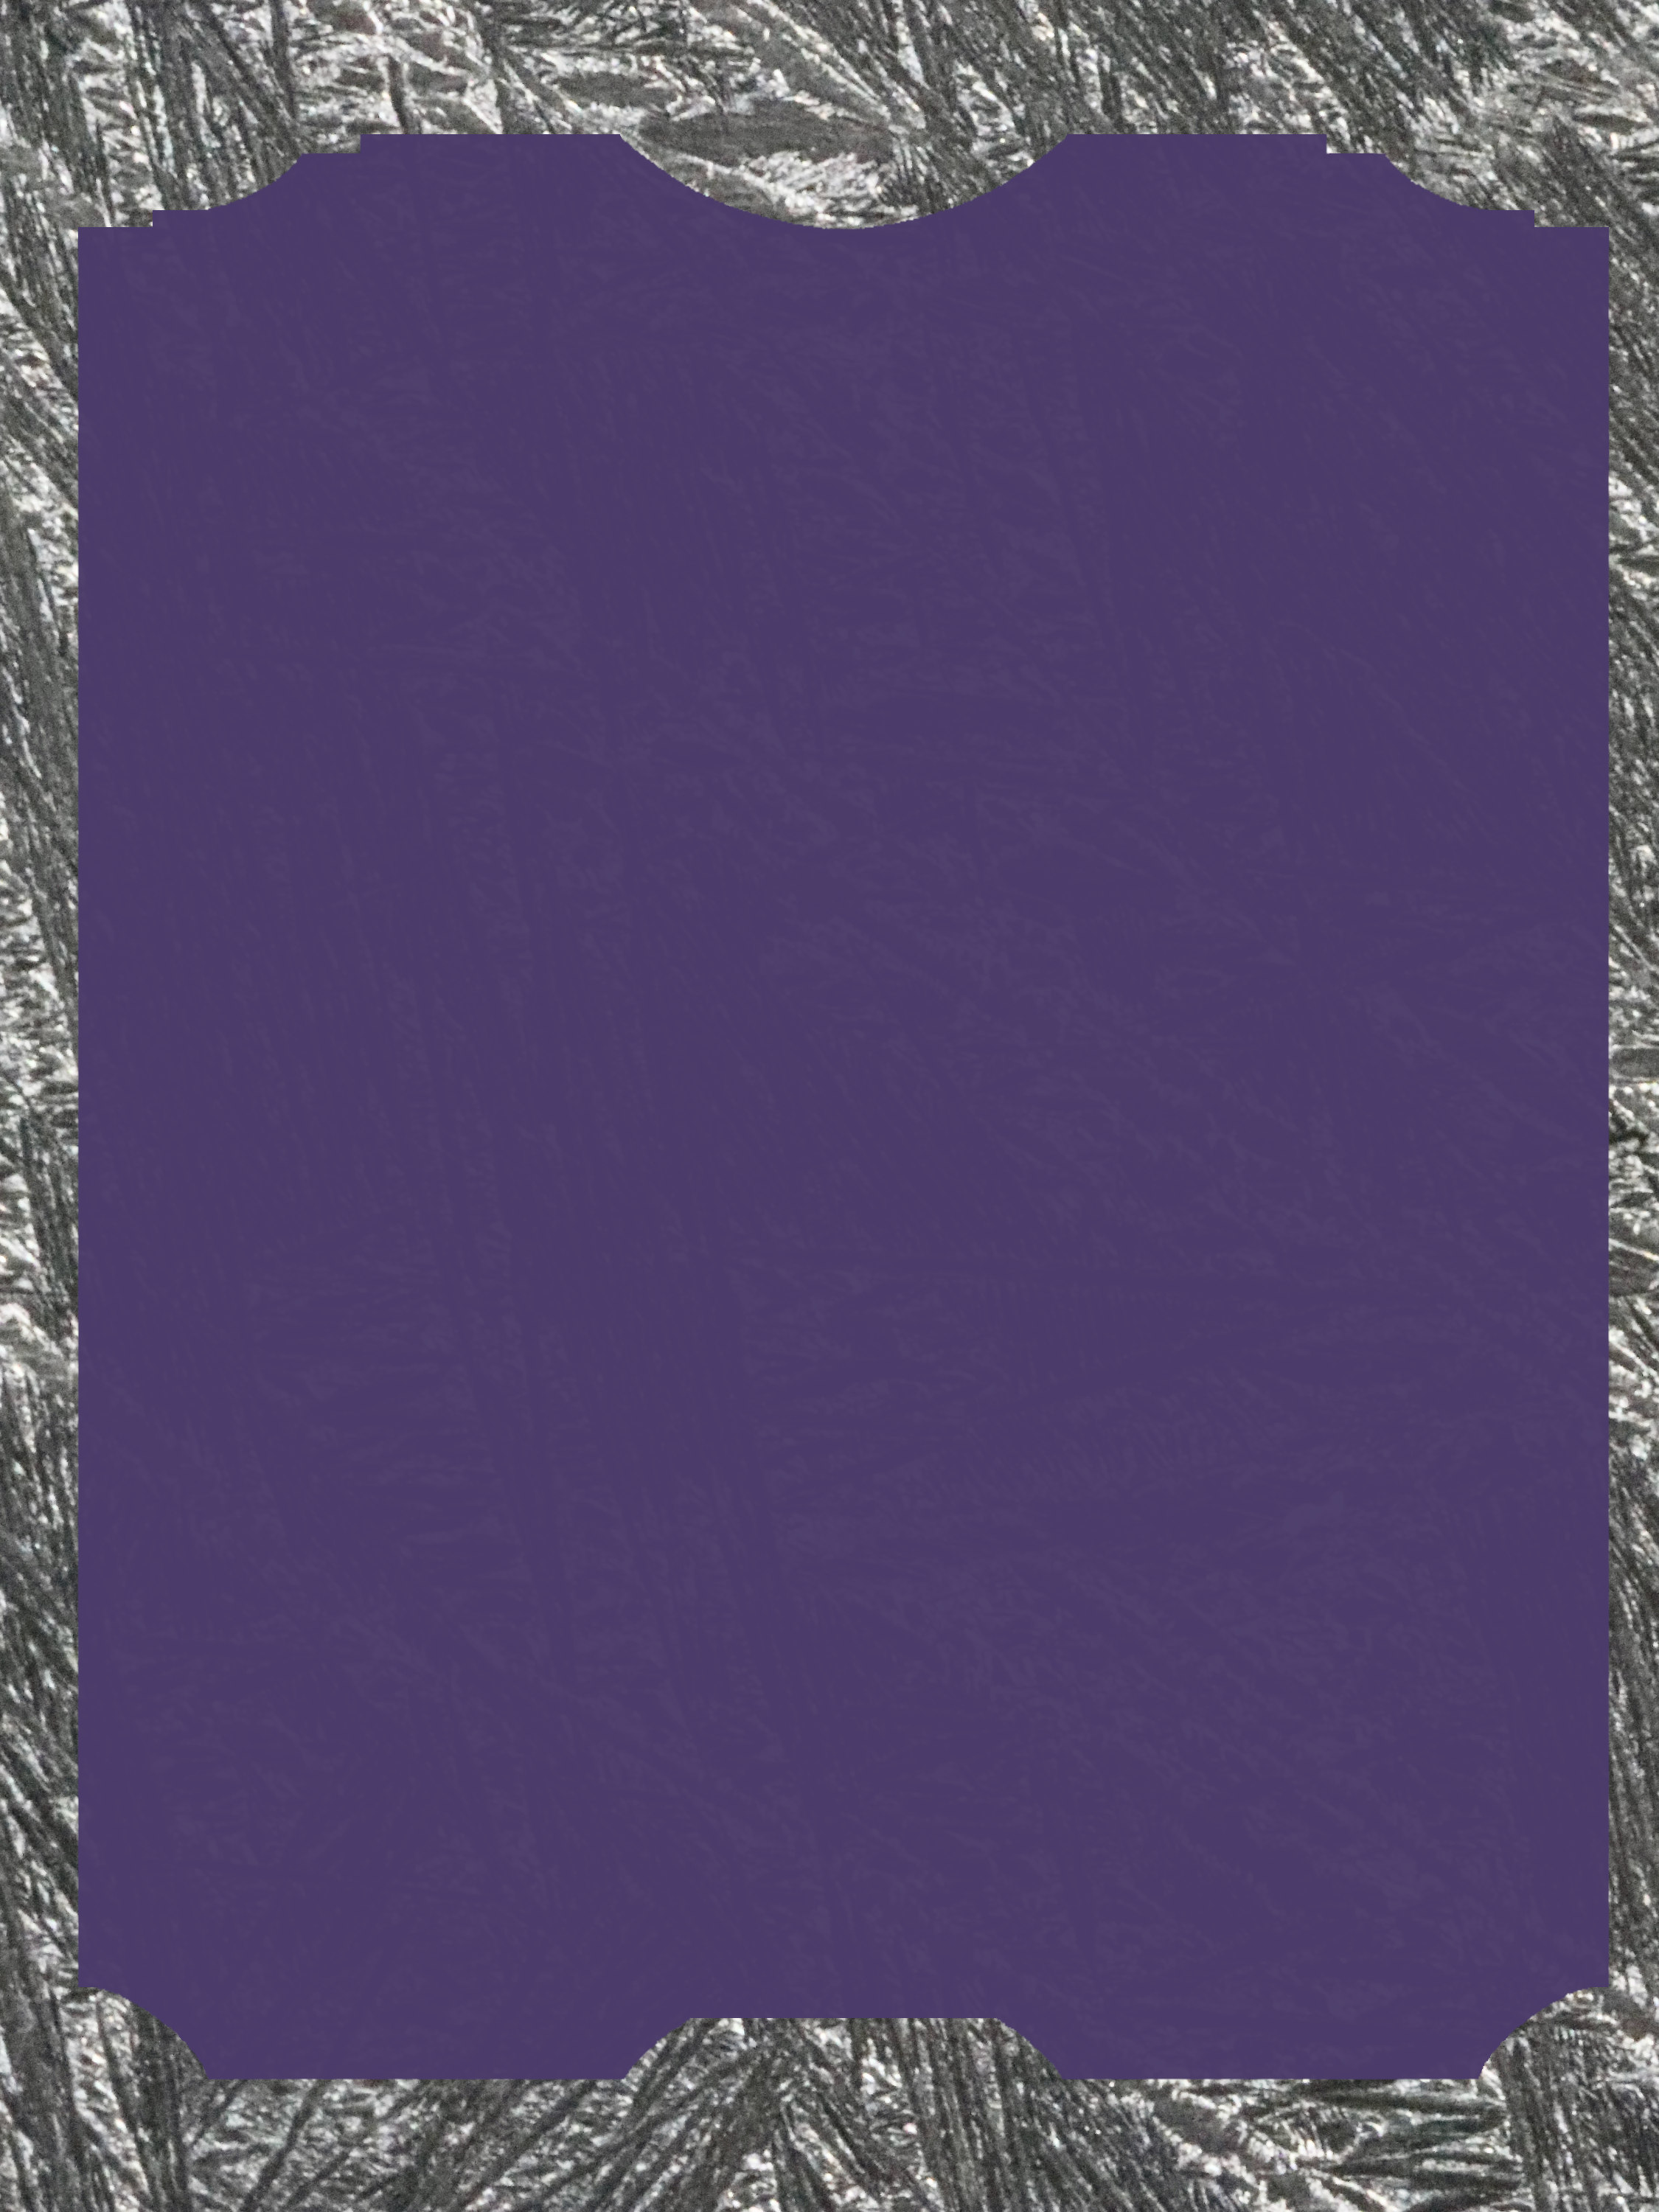
\includegraphics[width=\paperwidth,height=\paperheight]{etched.jpeg}}
\def\arraystretch{1.15}

\renewcommand\thefootnote{{\bfseries\color{myGreen}{\arabic{footnote}}}}
\let\oldfootnote\footnote
    \renewcommand{\footnote}[1]{\oldfootnote{{\large\bfseries\color{myGreen}#1}}}
\begin{titlepage} % Suppresses headers and footers on the title page
	\centering % Centre everything on the title page
	%\scshape % Use small caps for all text on the title page

	%------------------------------------------------
	%	Title
	%------------------------------------------------
	
	\rule{\textwidth}{1.6pt}\vspace*{-\baselineskip}\vspace*{2pt} % Thick horizontal rule
	\rule{\textwidth}{0.4pt} % Thin horizontal rule
	
	\vspace{1\baselineskip} % Whitespace above the title
	
	{\scshape\Huge "Uber den Ursprung der Meteorsteine.}
	
	\vspace{1\baselineskip} % Whitespace above the title

	\rule{\textwidth}{0.4pt}\vspace*{-\baselineskip}\vspace{3.2pt} % Thin horizontal rule
	\rule{\textwidth}{1.6pt} % Thick horizontal rule
	
	\vspace{1\baselineskip} % Whitespace after the title block
	
	%------------------------------------------------
	%	Subtitle
	%------------------------------------------------
	
	{\Large\scshape von P. A. Kesselmeyer.} % Subtitle or further description
	
	\vspace*{1\baselineskip} % Whitespace under the subtitle
	% Subtitle or further description
    
	%------------------------------------------------
	%	Editor(s)
	%------------------------------------------------
    \vspace*{\fill}

	\vspace{1\baselineskip}

	{\small\scshape Frankfurt a. M. 1860.}
	
	{\small\scshape{Druck und Verlag von Heinrich Ludwig Br"onner.}}
	
	\vspace{0.5\baselineskip} % Whitespace after the title block

    \scshape Internet Archive Online Edition  % Publication year
	
	{\scshape\small Namensnennung Nicht-kommerziell Weitergabe unter gleichen Bedingungen 4.0 International} % Publisher
\end{titlepage}
\setlength{\parskip}{1mm plus1mm minus1mm}
\clearpage
\Large
\tableofcontents
\clearpage
\section*{}
\hspace*{5mm}A. bedeutet: Arago, Astronomie populaire; Paris u. Leipzig 1857.

B. bedeutet: Buchner, die Feuermeteore, insbesondere die Meteoriten; Gie"sen 1859.

CR. bedeutet: Comptes rendus de l’academie des sciences a Paris.

G. bedeutet: Gilberts Annalen.

K. bedeutet: K"amtz, Lehrbuch der Metereologie; Halle 1836.

P. bedeutet: Poggendorffs Annalen.

RPG. bedeutet: Greg, an Essay on Meteorites, 1855.

S. bedeutet: Shepard, Catalogue of the Meteoric Collection of Charles Upham Shepard; New-Haven 1860.

SJ. bedeutet: Sillimans American Journal,

W. bedeutet: Haidinger, die Meteoriten des k. k. Hof-Naturalien-Kabinetts am 30. Mai 1860.

WA. bedeutet: Sitzungsberichte der mathematisch-naturwissenschaftlichen Klasse der k. Akademie in Wien.
\paragraph{}
Die Frage, woher wohl jene eigent"umlichen mineralogischen Gebilde stammen m"ogen, die von Zeit zu Zeit teils als v"ollig gediegene Eisenmassen, teils unter der Form von Basalt- und Dolerit-"ahnlichen Gesteinen, stets aber unter den auffallendsten Naturerscheinungen auf unsere Erde herabzufallen pflegen, musste mit Notwendigkeit von jeder die Geister besch"aftigen. Jene mittelalterliche Ansicht, dass solche Donnerkeile — wie man sie nannte — als Zeichen g"ottlichen Zornes mit unseren gew"ohnlichen Blitzschlagen vom Himmel kamen, konnte sich nat"urlich nur so lange halten, als man, in Folge eines wenig erleichterten Verkehres, die meisten dieser Tatsachen nur vom H"orensagen oder aus alten Chroniken kannte. Als aber mit der Zeit die Zahl wirklich beobachteter Meteorsteinf"alle sich stets mehrte; als alle Nachrichten und zwar aus den verschiedensten L"andern Europas, darin "ubereinstimmten, dass sie meistenteils gerade bei v"ollig heiterem und wolkenlosem Himmel sich ereigneten: da konnte eine solche Ansicht nicht l"anger mehr bestehen. "Ahnlich musste es einer anderen Erkl"arungsweise ergehen, wonach namentlich die Gediegen-Eisenmassen nichts Anderes sein sollen, als vom Blitz getroffene und eben dadurch innerlich wie "au"serlich ver"anderte gew"ohnliche Eiseng"ange\footnote{G. 14. 1803. Fol. 55.} unserer Erde. Auch sie musste zerfallen, nachdem man das Herabkummen gl"uhender Eisenmassen nicht allein wirklich beobachtet, sondern auch bemerkt hatte, dass fast alle f"ur meteorisch zu haltenden gediegenen Eisenmassen gerade vorzugsweise in solchen Gegenden sich vorfinden, wo weit und breit keine sonstigen Eisenlager vorhanden sind. Darum konnte denn auch nach allen diesen Tatsachen "uber den wirklich "uberirdischen Ursprung dieser r"atselhaften Gesteine kein Zweifel mehr obwalten. Aber wie und woher kommen sie in jene luftigen H"ohen, aus denen sie, begleitet von so ungew"ohnlichen Erscheinungen, auf unsere Erde herabfallen? Diese Frage einmal angeregt, konnte der zun"achst liegende Gedanke wohl kaum ein anderer sein, als sie f"ur Felsbruchst"ucke zu halten, welche durch die Gewalt irischer Vulkane in die H"ohe geschlendert, nun in Folge ihrer Schwere wiederum in anderen Gegenden herabfallen. Allein die gro"se Entfernung der Niederf"alle von den zun"achst liegenden, noch jetzt t"atigen Feuerbergen, so wie das ungeheure Gewicht einzelner dieser Steine, mussten sofort gegen eine solche Annahme sprechen. Auch die Vergleichung der Steine selbst mit denen, wie sie in der N"ahe unserer Vulkane wirklich sich vorfinden, erschien einer solche Annahme nicht g"unstig.

Auf der Erde also — so schien es nach allem Diesem — war ihr Ursprung nicht zu suchen. Von Himmel schienen sie in der Tat zu kommen. Was war daher wohl wahrscheinlicher, als sic von nun an f"ur fremde Eindringlinge, f"ur die handgreiflichen, tast- und f"uhlbaren Boten einer uns unbekannten und unzug"anglichen Welt zu halten? Aber wo in dem weiten Weltenall sollte man ihre wirkliche Heimat suchen? Bei diesen Gedanken einmal angelangt, lag nichts n"aher, als die Blicke nach dem Monde zu lenken, dem uns bekanntesten und n"achsten aller Himmelsk"orper. Nach den Beobachtungen der Astronomen schien es nicht zu bezweifeln, dass t"atige Vulkane auf seiner Oberfl"ache sich befinden. Auch hielt man es nach angestellten Berechnungen nicht f"ur unm"oglich, dass dieselben im Stande sein d"urften, Felsenmassen bis in eine solche Entfernung in die H"ohe zu schleudern, dass sie — die Grenze der Anziehung ihres eigenen Himmelsk"orpers "uberschreitend und derjenigen unserer Erde nun verfallend — in immer rascherem Falle endlich auf diese Letztere selbst herabzust"urzen gezwungen seien. Die bedeutendsten Naturforscher, wie Laplace, Olbers, Berzelius\footnote{P. 33. 1834. Fol. 1 u. 113. P. 36. 1835. Fol. 161.} und Andere, huldigten dieser Ansicht. Der verschiedenartige Charakter der einzelnen Meteorsteine erkl"arte sich hiernach einfach und nat"urlich durch die geognostische Verschiedenheit der einzelnen Mondgebirge. Die Feuererscheinung, das Ergl"uhen der ganzen Masse kurz vor dem Niederfall, war eine Folge der Reibung, welche der Eindringling durch die in Folge seines Falles gewaltsam zusammengepresste Luft erlitt. Selbst die Beobachtung, dass alle diese fallenden K"orper trotz ihrer weiten Herkunft am Ende doch nur mit der gew"ohnlichen Fallgeschwindigkeit auf unserer Erde anlangten, schien in dieser gewaltsamen Zusammenpressung der Luft und in dem durch sie hervorgerufenen Widerstande ihre nat"urliche Erkl"arung zu finden.

Allein ungeachtet aller dieser Gr"unde vermochte diese Ansicht doch nicht, nach allen Seiten hin vollst"andig zu gen"ugen. Die ungeheure Gewalt der Mondvulkane, wie sie zu einer solchen Annahme n"otig war, erschien Vielen nicht minder r"atselhaft als die ganze Erscheinung selbst, welche durch sie ihre Erkl"arung finden sollte. Daher versuchte denn Chladni eine neue Bahn, und trat allen bisherigen Ansichten mit der Theorie von dem kosmischen Ursprung\footnote{G. 13. 1803. Fol. 350. G. 57. 1817. Fol. 121. G. 68. 1821. Fol. 369. P. 36. 1835. Fol. 176.} aller meteorischen Gesteine gegen"uber. Alle vom Himmel fallenden K"orper, alle Meteorsteine, alle Sternschnuppen, Feuerkugeln u. s. w. stammten nach ihm aus dem weiten Weltenraume, wo sie, entweder schon geballt als feste planetarische K"orper, oder noch ungeballt als planetarische Dunst- und Nebelmassen, ihre uns unbekannten Bahnen beschreiben. Gelangt --- so nahm er an --- einer dieser "`Weltsp"ane"' in die N"ahe eines gr"o"seren Himmelsk"orpers, so wird er von diesem aus seiner Bahn herausgezogen, bis er, dieser "uberm"achtigen Anziehung immer mehr folgend, endlich nach denselben Gesetzen wie jene Ausw"urflinge des Mondes in immer unwiderstehlicherem Fluge auf den anziehenden Himmelsk"orper selbst herabst"urzt, um nie und nimmermehr in seine fr"uhere Bahn zur"uckzukehren. Das namentlich bei Feuerkugeln "ofters beobachtete sogenannte Rikoschettieren, dies sprungweise sich Auf- und Ab-bewegen galt ihm als ein unverkennbares Zeichen des wirklichen Eindringens von au"sen in die dichteren Schichten unseres irdischen Dunstkreises: es war das von unserer Erde aus betrachtete Abprallen der eindringenden Masse von der im Vergleich zum Welt"ather weit dichteren, elastisch-fl"ussigen Oberfl"ache unserer Atmosph"are. Das pl"otzliche Ergl"uhen erkannte er ebenfalls als eine Folge der durch Reibung und Kompression der Luft erzeugten Warme, und das h"aufig wahrgenommene Anschwellen der feurigen Kugel f"ur ein durch eben diese Hitze erzeugtes blasen"ahnliches Aufschwellen der eingedrungenen Masse, dessen endliche Folge das Zerplatzen und das Herabfallen der in ihr enthaltenen oder gebildeten Steine sein musste.

Diese Ansicht Chladnis gewann sich bald viele und sehr bedeutende Anh"anger. Die angesehensten Naturforscher traten ihr bei, und auch noch jetzt ist sie die am Meisten verbreitete. Allein nichtsdestoweniger erhoben sich auch gegen sie schon fr"uhzeitig gar manche und gewiss nicht zu missachtende Bedenken. Die Vermutung, dass trotz der scheinbaren Unm"oglichkeit unsere irdische Atmosph"are vielleicht dennoch die Grundstoffe sollte liefern k"onnen, aus denen diese "`Luftsteine"' gewoben, war schon fr"uhe hier und dort ge"au"sert worden. Als feste Massen k"onnen sie sich freilich nicht in derselben aufhalten. Ob dieses aber nicht im dunst- oder gasf"ormigen Zustand m"oglich w"are? Diese Frage war, wenn gleich Anfangs erfolglos, doch schon ziemlich fr"uhe aufgestellt worden. So hielt Musschenbroek\footnote{G. 14. 1803. Fol. 55.} die Meteorsteine f"ur schwefelhaltige D"ampfe aus unseren irdischen Vulkanen, und Dominicus Tata\footnote{G. 6. 1800. Fol. 156.} "au"serte sich bei Gelegenheit des Steinfalles von Siena dahin, dass derselbe kiesigen Materialien seinen Ursprung zu verdanken haben d"urfte, welche sich in Dampfgestalt von unserer Erde erhoben, und innerhalb unserer Atmosph"are durch elektrische und andere Kr"afte in den festen Zustand gebracht worden seien. Auch Patrin\footnote{G. 33. 1809. Fol. 189.} erkl"arte die Bildung der Meteorsteine geradezu f"ur identisch mit der Bildung derjeniger Massen, die auch unsere irdischen Vulkane auswerfen, d. h. f"ur chemische Verbindungen verschiedener, durch vulkanische Hitze in Gasgestalt "ubergef"uhrter Substanzen. Sp"ater waren es namentlich Wrede, Egen und von Hof, welche sich in "ahnlicher Weise gegen den kosmischen Ursprung erkl"arten. Wrede\footnote{G. 14. 1803. Fol. 55.} wies darauf hin, wie unrecht man getan, Sternschnuppen, Steinf"allen, Feuermeteoren, Sand- und Staubregen, --- allen den gleichen kosmischen Ursprung zuzuschreiben. Letztere, die Sand- und Staubregen, so wie die blo"s leuchtenden Feuerkugeln erkl"arte er f"ur Erscheinungen, die entschieden unserer irdischen Atmosph"are angeh"orten. Aber auch f"ur die Meteorsteine erkannte er wenigstens die M"oglichkeit eines irdischen Ursprungs an, und es erschien ihm hierbei als v"ollige unerkl"arlich, wie die nemlichen w"agbaren Stoffe, die nach der kosmischen Lehre innerhalb unserer irdischen Atmosph"are nicht sollten vorhanden sein k"onnen, dennoch in dem den freien Weltraum erf"ullenden "Ather, also in einem noch unendlich feineren Medium, sollten anzutreffen sein. Daher war denn auch Egen\footnote{G. 72. 1822. Fol. 375.} vornehmlich bem"uht, durch statistische Berechnungen nachzuweisen, welche ungeheure Mengen fester Stoffe allj"ahrlich in unseren H"uttenwerken sich verfl"uchtigen, und somit wirklich in Gasgestalt in unsere Atmosph"are "ubergehen. Ebenso wies er darauf hin, dass Pflanzen, die in destilliertem, mithin von fremden Stoffen v"ollig freiem Wasser leben, nichtsdestoweniger Erd- und Eisenteile in ihrem Inneren enthalten: ein Beweis, dass diese Stoffe in der die Pflanzen umgebenden Luft, aus welcher sie sie allein aufzunehmen im Stande waren, auch notwendig enthalten sein m"ussen. Von Hof\footnote{P. 36. 1835. Fol. 161.} suchte endlich vorzugsweise die Ansicht zu bek"ampfen, dass die meteorischen Gesteine von au"sen her als bereits feste Massen in unsere Atmosph"are eindr"angen. Denn --- so hob er nicht ohne Grund hervor --- w"are das beobachtete Ergl"uhen wirklich eine Folge jener ungeheuren Reibung des eindringenden festen K"orpers an den einzelnen Luftteilchen unserer Atmosph"are: dann m"usste dieses Ergl"uhen auch notwendig immer st"arker werden, je mehr der fallende K"orper der Oberfl"ache unserer Erde sich n"ahert. Denn mit der gr"o"seren N"ahe an unserer Erde w"achst nicht allein die Geschwindigkeit des Falles, sondern auch die Dichtigkeit der Luft, mithin die Reibung selbst und ihre erhitzende Wirkung auf den im Fall begriffenen K"orper. Dem ist aber nicht so. Nicht bei seiner Ankunft auf der Erde zeigt sich der Stein in seiner h"ochsten Gluth, sondern im Gegenteil vorher, und zwar gerade in den h"ochsten und d"unnsten Schichten unserer Atmosph"are. Ebenso wies er darauf hin, dass, wenn auch durch gewaltsame Zusammenpressung von Luft, wie z. B. in dem pneumatischen Feuerzeuge, eine gro"se Hitze erzeugt werde, dies letztere Beispiel mit dem vorliegenden Fall doch in keiner Weise verwechselt werden d"urfe. Im pneumatischen Feuerzeug sei die Luft von allen Seiten fest eingeschlossen; in freier Atmosph"are dagegen --- ein Punkt, auf den auch Scherer\footnote{G. 31. 1809. Fol. 1.} schon aufmerksam gemacht hatte --- verm"ochten die einzelnen Teilchen bei ihrer gro"sen Beweglichkeit sofort vor dem fallenden K"orper nach allen Seiten hinzuentweichen. Aber auch die Ansicht einer Bildung der Gesteine einzig und allein aus Stoffen unserer Atmosph"are schien ihn nicht zu befriedigen. Daher neigte er denn auch mehr zu der schon von Chladni ge"au"serten Ansicht von den kosmischen Urnebeln hin, so wie zu der M"oglichkeit eines gegenseitigen Austausches der Stoffe zwischen dem freien Weltraum und unserer irdischen Atmosph"are. So viel aber --- f"ugt er endlich hinzu\footnote{P. 36. 1835. Fol. 176.} --- gehe aus Allem hervor, dass in demselben Augenblick, wo in unserer Atmosph"are die Lichtentwicklung und die Explosion stattfindet, eine tats"achliche chemisch-physische Operation vor sich gehe, kraft welcher aus dem ergl"uhten Urstoff ein neuer K"orper sich bilde, und dieser neue K"orper sei der herabfallende Meteorstein. Inmitten unserer Atmosph"are sei er jedenfalls gebildet: von au"sen k"onne er fertig nicht gekommen sein.

So sehen wir, wie die verschiedenartigsten Ansichten sich "au"serten, sich bek"ampften, und gegenseitig zur Geltung zu gelangen suchten. Man ist von den Massen geballter und ungeballter Materien im Weltraum, "uber Nebelflecke und durch Sternschnuppenschw"arme, "uber gro"se und "uber kleine Planeten herabgestiegen bis zu den Meteorsteinen und Feuerkugeln, ja herunter bis zu unseren Blut- und Staubregen, einzig und allein um f"ur die Meteorsteine einen kosmischen Ursprung zu begr"unden. F"ur die Blut- und Staubregen aber ist eine solche au"serirdische Herkunft gewiss mehr als zu bezweifeln. Eine wirkliche Identit"at zwischen Feuerkugeln und Sternschnuppen ist ebenfalls noch keineswegs erwiesen. Denn wenn es gleich hier und dort vorgekommen, dass bei sehr lebhaften Sternschnuppenschw"armen gleichzeitig auch Feuerkugeln beobachtet worden sind: so lehrt doch die Erfahrung, dass Feuerkugeln im Allgemeinen unbegleitet von Sternschnuppen, und auch nicht, wie diese, an bestimmte Perioden gebunden am Himmelszelt erscheinen.\footnote{A. v. Humboldt. Kosmos 3. Fol. 609 u. 610. RPG Fol. 10 u. 16.} Ber"ucksichtigen wir "uberdies auch noch die nach angestellten Beobachtungen langsame Bewegung der Feuerkugeln im Vergleich zu der der Sternschnuppen, so wie die nach aller Wahrscheinlichkeit weit gr"o"sere Entfernung dieser letzteren von der Oberfl"ache unserer Erde: so darf ein gemeinschaftlicher Ursprung der Feuerkugeln --- namentlich derer, die in der Luft zergehen, ohne Steine zu uns herabzusenden --- und der zu bestimmten Perioden unsere Erdbahn durchkreuzenden Sternschnuppen gewiss f"ur jetzt noch sehr bezweifelt werden. Allein auch f"ur solche Feuerkugeln, die wirklich in Steine sich aufl"osen, haben wir gesehen, dass nicht unerhebliche Gr"unde gegen die Annahme eines au"serirdischen Ursprunges vorhanden sind. Zu diesen Gr"unden ist vorzugsweise der schon oben erw"ahnte Umstand zu rechnen, dass das sofortige Ergl"uhen der Steine --- wenn diese wirklich in einem bereits festen Zustand von au"sen her in unsere Atmosph"are eindr"angen --- gerade in den obersten und darum auch noch allerd"unnsten Schichten unseres Dunstkreises wohl kaum nach den uns bekannten nat"urlichen Gesetzen eine befriedigende L"osung finden kann. Denn wollte man auch annehmen, dass jene meteorischen Massen zwar wohl im festen Zustand, aber nicht als fest zusammenh"angende K"orper, sondern nur im Zust"ande feinster Verteilung, gleichsam als ein kosmischer Staub oder als ein kosmisches Pulver, im Weltraum sich bef"anden, und auch in solcher Weise nun in die obersten Schichten unserer Atmosph"are gelangten: so lie"se sich hierdurch die gro"se Entz"undlichkeit solcher pulverf"ormigen Massen beim Eintritt in die sauerstoffreichere Atmosph"are unserer Erde zwar befriedigender erkl"aren; allein andere Schwierigkeiten w"urden daf"ur auftauchen. F"ur das wirkliche Vorhandensein fester und dabei doch au"serordentlich kleiner Weltk"orper innerhalb unserer Sonnensysteme sprechen unsere kleinen Planeten. Auch die Sternschnuppenschw"arme scheinen darauf hinzudeuten. Wir kennen in gleicher Weise kosmische D"unste und Nebelflecken, die zum Theil, selbst bei den st"arksten Vergr"o"serungen, noch in keine bestimmten Sternhaufen aufgel"ost werden konnten. Aber von solchen kosmischen Staub- und Pulvermassen, wie sie zur Erkl"arung jener lebhaften Entz"undbarkeit gerade in den obersten und d"unnsten Gebieten unserer Atmosph"are notwendig sein w"urden, gewahren wir nirgends die allergeringste Andeutung. Zudem muss es aber auch weiterhin sehr r"atselhaft bleiben, wie durch die blo"se Anziehung unserer Erde planetarische K"orper, die gleich unserem eigenen Erdk"orper mit planetarischer Geschwindigkeit um die Sonne sich bewegen, von jenem sollten g"anzlich zu sich herabgezogen werden; w"ahrend doch sonst die Himmelsk"orper selbst in ihrer gr"o"sten N"ahe sich h"ochstens nur in ihrer gegenseitigen Geschwindigkeit ein wenig aufhalten, oder in ihrem Laufe nur unbedeutend aus ihren gew"ohnlichen Bahnen sich abzulenken verm"ogen. Wollte man aber annehmen, ein solches Herabst"urzen des kleineren Weltk"orpers auf den gr"o"seren sei in Bezug auf unsere Meteorsteine deshalb doch wohl denkbar, weil diese ungew"ohnlich kleinen Miniaturweltk"orperchen wohl auch in einer weit gr"o"seren N"ahe bei unserer Erde ihre Bahnen beschreiben: so w"urde eine solche Annahme doch jedenfalls nur allein f"ur die spezifisch leichteren unter unseren Meteorsteinen eine Geltung haben k"onnen. Denn nach einem bekannten Naturgesetze befinden sich die dichteren und spezifisch schwereren Planeten auch in gr"o"serer N"ahe bei der Sonne als die spezifisch leichteren. Die mittlere Dichtigkeit des Merkurs gleicht der des Goldes oder des Platins; die der Venus derjenigen des Glases; der Erde des Flussspates u. s. w.\footnote{Littrow. Wunder des Himmels. 3. Fol. 68.} Die metallischen dichten Eisenmassen, welche von Zeit zu Zeit ebenfalls auf unsere Erde herabst"urzen, mussten demnach notwendig in einer so bedeutenden Entfernung von unserer Erde ihre Bahnen beschreiben, dass f"ur sie eine solche "uberm"achtige Anziehung unserer Erde wohl kaum f"ur wahrscheinlich zu halten sein d"urfte. Sollten sie durch Anziehung wirklich auf einen anderen Planeten hinabzust"urzen gezwungen werden, so m"usste f"ur sie der anziehende Himmelsk"orper gewiss weit eher der ihnen nicht allein n"ahere, sondern auch dichtere Merkur sein, als die von ihnen entferntere Erde. Neigt man sich dagegen aber zu der Ansicht einer Entstehung aus blo"sem Urnebel hin, so bleiben nicht allein die R"atsel wegen des Herausrei"sens aus der urspr"unglichen Umlaufsbahn dieselben; sondern es h"alt auch au"serdem schwer, den Grund daf"ur zu finden, weshalb diese Nebelmassen, die selbst in dem nach angestellten Berechnungen weit "uber 100$^\circ$ kalten Weltraum noch nicht erstarrt sind, nun mit einem Male in den festen Zustand "ubergehen, sobald sie in unserer Atmosph"are, also in einem Mittel anlangen, das wohl kaum noch k"alter sein d"urfte als dasjenige, aus welchem sie stammen, --- ja wo sie in Folge der durch ihre Reibung angeblich erzeugt werden sollenden Hitze sofort in eine solche Gluth versetzt werden, dass eine jede Idee an eine auf solchem Wege zu bewirkende Verdichtung gasf"ormiger Stoffe --- wie es scheint --- von vornherein ausgeschlossen werden muss. Aber auch gegen die Annahme, als dr"angen unsere Meteorsteine in bereits festem Zustand aus dem freien Weltraum in den Dunstkreis unserer Erde ein, erhebt sich aus astronomischen R"ucksichten eine weitere, bisher zwar noch wenig beachtete, aber doch, wie es scheint, nicht ganz unwesentliche Schwierigkeit. Beschreiben nemlich unsere Meteorsteine als bereits feste planetarische Massen innerhalb unseres Sonnensystems ihre uns unbekannten Bahnen um die Sonne: dann m"ussen sie notwendig auch alle dieselbe Richtung von West nach Ost einhalten, der alle "ubrigen Planeten folgen, und die Ebenen ihrer Bahnen m"ussen gleich denjenigen aller "ubrigen Planeten mit der ungef"ahren Richtung des Tierkreises "ubereinstimmen. Au"serdem haben wir alsdann --- wie oben bereits angedeutet, --- allen Grund, anzunehmen, dass die spezifisch schwereren Gesteinsmassen, also namentlich die meteorischen Eisenmassen, n"aher bei der Sonne, die spezifisch leichteren dagegen weiter von der Sonne als unsere Erde ihre Bahnen beschreiben. Die der Sonne n"aheren Himmelsk"orper, m"ogen sie nun gro"s oder klein sein, beschreiben aber bekanntlich mit gr"o"serer Schnelligkeit ihren Lauf um die Sonne, als die von der Sonne entfernteren. Wenn daher unsere Erde mit irgendeinem dieser Miniaturweltk"orper in solche N"ahe kommen soll, dass sie im Stande sei, ihn verm"oge ihrer Anziehung zu sich herabzuziehen: dann m"usste sie es sein, welche alle langsamer sich bewegenden, d. h. mit anderen Worten alle spezifisch leichteren Massen in ihrem Laufe einholt, unterdes sie von allen sich schneller bewegenden, d. h, spezifisch schwereren, eingeholt wird. Daraus w"urde nun aber mit Notwendigkeit auch folgen, dass, w"ahrend alle spezifisch schwereren Meteorsteine und also namentlich alle meteorischen Gediegen-Eisenmassen stets von Westen her auf unserer Erde anlangen w"urden, im Gegenteil alle spezifisch leichteren, weil von unserer schneller sich bewegenden Erde in ihrem Laufe "uberholt, dem "au"seren Anscheine nach von Osten her zu uns gelangen m"ussten. Die Erfahrung best"atigt dieses aber keineswegs. Im Gegenteil finden wir, dass die Meteorsteine so ziemlich aus allen Himmelsgegenden bei uns anlangen. Ja selbst in Bezug auf die Gediegen-Eisenmassen ersehen wir aus den uns erhaltenen Aufzeichnungen, dass auch sie nicht einmal die gleiche und best"andige Richtung einhalten: der Meteor-Eisenfall von Hraschina (1751) kam aus Nordwesten\footnote{WA. 35. 1859. Fol. 17 u. 18.}; der von Braunau (1847) dagegen aus Nordosten.\footnote{P. 72. 1847. Fol. 170.} Bei dunst- und gasf"ormigen Massen m"ogen wir uns nun zwar wohl denken, dass sie --- innerhalb unserer Atmosph"are von Winden und Luftstr"omungen hin- und hergetragen --- leicht und h"aufig die urspr"ungliche Richtung ihres Laufs verlassen, und darum auch so ziemlich aus allen m"oglichen Wind- und Himmelsgegenden nach eingetretener Verdichtung zu uns herabzugelangen im Stande sind. Bei festen Massen dagegen, die mit einer schon an und f"ur sich planetarischen Geschwindigkeit in unseren Dunstkreis eindringen, und deren Geschwindigkeit "uberdies auch noch in Folge ihres Falles, ungeachtet des Widerstandes der nach allen Seiten hin frei entweichenden Luft, eine fortw"ahrend sich beschleunigende sein muss, d"urfte die Annahme einer "ahnlichen Einwirkung von irdischen Wind- und Luftstr"omungen gewiss von vornherein als unstatthaft sich erweisen. Die Gewalt auch der heftigsten Orkane muss als verschwindend erscheinen, gegen"uber der ungeheuren Heftigkeit und Schnelligkeit des Falles, womit aus dem freien Weltraum stammende feste planetarische K"orper in unseren Dunstkreis eindringen. An ein Herausrei"sen aus ihrer nat"urlichen Richtung durch lokale irdische Verh"altnisse darf daher bei ihnen gewiss auch nicht im Entferntesten gedacht werden.

Sollte es nun, nach all diesen Zweifeln und Ungewissheiten, nicht zweckm"a"sig und erlaubt erscheinen, auch wieder einmal den umgekehrten Weg wie zeither zu versuchen? d. h. anstatt von den uns entferntesten und allerfremdesten Gegenst"anden, von den Planeten und ihren Urmaterien auszugehen, vielmehr mit den uns bekanntesten und n"achsten meteorologischen Tatsachen, wie sie fortw"ahrend hier auf Erden uns umgeben, zu beginnen, und von ihnen aus uns allm"ahlich zu jenen uns noch unbekannteren Naturerscheinungen zu erheben, mit deren Erkl"arung wir uns eben jetzt besch"aftigen?

Die n"achste Br"ucke, um von der Oberfl"ache unserer Erde in jene luftigen R"aume zu gelangen, in welchen jene eigent"umlichen Ereignisse stattfinden, bilden wohl jedenfalls die w"asserigen D"unste unserer Atmosph"are.\footnote{Shepard, Report on American Meteorites Fol. 52.} Sie sind die ersten und uns zun"achst liegenden Beweise einer ununterbrochenen Wechselwirkung zwischen Stoffen unserer Erde und der diese umlagernden Dunsth"ulle. In unsichtbarer Gasgestalt erheben sie sich von unserer Erde, werden durch Winde und Luftstr"omungen in weite Fernen getragen, durch K"alte in den h"oheren Regionen unserer Atmosph"are wiederum verdichtet, um endlich in Gestalt von Regen, Schnee und Hagel wieder zu uns herabzugelangen. Zwar finden diese "Uberg"ange ohne jene eigent"umlichen Verbrennungs- und Feuererscheinungen statt, wie wir solche stets bei der Bildung der Meteorsteine gewahren. Allein die innere Natur der diesen beiden Erscheinungen zu Grunde liegenden Stoffe scheint hinreichend zu sein f"ur die Erkl"arung dieser Verschiedenheit. Und will man einwenden, dass Regen und Hagel nur in verh"altnism"a"sig kleineren Tropfen und K"ornern zur Erde k"amen, die meteorischen Gesteine dagegen meistenteils in gro"sen und selbst ungeheuren Massen: so wird eine n"ahere Pr"ufung des Tatbestandes uns zeigen, dass auch in dieser Beziehung zwischen beiden Naturerscheinungen kein so gro"ser Unterschied herrscht, als es in dem ersten Augenblick wohl den Anschein hat. Als Regen kommt das atmosph"arische Wasser freilich nur tropfenweise zur Erde. Aber selbst diese Tropfen sind oft sehr verschieden an Gr"o"se; und richten wir unsere Blicke auf das auf unsere Erde herabkommende meteorische Eisen --- die einzigen Massen, welche, wenn auch nicht v"ollig fl"ussig, so doch in mehr oder minder weichem Zustande bei uns eintreffen---: so finden wir auch hier tats"achlich dieselbe Tropfenbildung wieder. Das Eisen von Hraschina\footnote{G. 50. 1815. Fol. 263. WA. 35. 1859. Fol. 364-373.} ist, wie die Berichte ausdr"ucklich melden, in Gestalt "`feuriger Ketten,"' d. h. in nicht zusammenh"angender, sondern in zerrissener, tropfen"ahnlicher Weise auf unserer Erde angelangt. Aus der Bezeichnung "`feurige Ketten"' geht hervor, dass diese Tropfen jedenfalls weit gr"osser gewesen sei m"ussen, als unsere gew"ohnlichen Regentropfen: ein Umstand, der bei dem nicht v"ollig fl"ussigen, sondern nur halbweichen Zustande der fallenden Masse nicht zu verwundern ist. Das zerrissene, unzusammenh"angende Herabkommen, also das, was den Tropfen charakterisiert, sehen wir jedenfalls entschieden ausgepr"agt. Noch gr"osser aber wird die "Ahnlichkeit zwischen den w"asserigen Niederschl"agen unserer Atmosph"are und den Naturerscheinungen, welche uns besch"aftigen, wenn wir auf den Hagel unsere Blicke lenken. Die Meteorsteinchen im Gewicht von mitunter nur 2 Qu"antchen, welche 1803 in ungeheurer Menge zu l'Aigle\footnote{G. 15. 1803. Fol. 74 u. G. 16. 1804. Fol. 44.} herabgefallen sind, werden in Bezug auf Gr"o"se und Umfang den Vergleich mit unseren gew"ohnlichen Hagelk"ornern sehr wohl aushalten. Aber kennen wir nicht auch Schlossen von weit bedeutenderer Gr"o"se? 1767 fielen am Comer See\footnote{P. 13. 1828. Fol. 344.} Hagelk"orner bis zur Gr"o"se von H"uhnereiern, und 1819 zu Mayenne bis zu 15$^\prime$$^\prime$ Umfang. Und trotz dieser Gr"o"se wird gerade bei diesen letzteren von Delcross\footnote{G. 68. 1821. Fol. 323.} berichtet, dass es h"aufig nur Bruchst"ucke noch gr"o"serer, durch irgendeine innere Explosion schon w"ahrend des Niederfalls gewaltsam zerrissener Eismassen von Kugelgestalt gewesen seien: --- ein Umstand, der stark an das so h"aufig beobachtete Bersten der Meteorsteine in verschiedene kleinere Bruchst"ucke erinnert, bevor sie noch auf unserer Erde angelangt sind. Indessen sind die eben beschriebenen Hagelk"orner noch bei weitem nicht die gr"o"sten. Am 28. Mai 1802 fiel bei Puztemischel in Ungarn\footnote{G. 16. 1804. Fol. 75.} w"ahrend eines Hagelwetters ein Eisklumpen zur Erde, der 3 Fu"s L"ange, 3 Fu"s Breite und 2 Fu"s Dicke hatte; er ward auf 11 Zentner gesch"atzt. Ein zweiter hatte die Gr"o"se eines Reisekoffers. Doch die gr"o"ste vom Himmel gefallene Eismasse, die an Umfang und Gewicht wohl nur wenigen Meteorsteinen nachstehen d"urfte, ist diejenige, deren L. von Buch\footnote{G. 76. 1824, Fol, 342.} Erw"ahnung tut, indem er aus Heynes Tracts historical und statistical on India als eine wohlbeglaubigte Tatsache berichtet, dass sie zur Zeit des Tippoo Saheb nahe bei Seringapatam in Indien zur Erde gefallen sei. Sie war von der Gr"o"se "`eines Elephanten,"' und es vergingen trotz der Hitze des Landes 2 Tage, bis sie vollst"andig geschmolzen war. Zwar sind bei Hagel Massen von solcher Ausdehnung allerdings nur Seltenheiten. Dieser Umstand findet aber, im Vergleich mit den Meteorsteinen, sicherlich in der Verschiedenheit der zu Grunde liegenden Stoffe und vor Allem in der Ungleichheit ihrer inneren Dichte und der daraus hervorgehenden Verschiedenheit in der gegenseitigen Anziehung der einzelnen Massenteilchen seine hinl"angliche Begr"undung. --- Haben wir nun aber einmal mit Regen und Hagel begonnen: so ist der Schritt zu den ihnen sichtbarlich verwandten Blutregen\footnote{G. 64. 1820. Fol. 335.} nur ein kleiner. Hier haben wir schon einen metallischen Stoff, das Kobalt, und zwar in der Form von Chlorkobalt vor uns. Er muss zu der Zeit, wo der Regen sich bildet, und zwar ebenfalls in Dunstform, in unserer Atmosph"are notwendig in Wirklichkeit vorhanden sein. Einen weiteren Beweis, dass derartige metallische Stoffe wirklich bald mehr bald weniger in Gasgestalt in unserer Atmosph"are sich befinden, liefern die Hagelf"alle mit festen Metall- oder Steinkernen.\footnote{G. 72. 1822. Fol. 436. G. 31. 1809. 307. u. P. 28. 1833. Fol. 570.} Hier wurden offenbar die durch eintretende K"alte sich verdichtenden Metalld"unste die anziehenden Mittelpunkte, um welche die ebenfalls aus der Luft sich ausscheidenden Wasserteilchen sich ansammelten, und auf diese Weise nun eine "au"sere Eish"ulle um dieselben bildeten.

Nun w"are aber die wichtigste Frage, wie solche metallische D"unste wohl von unserer Erde aus in unsere Atmosph"are zu gelangen verm"ogen, und es zeigen sich uns hierf"ur vornehmlich zwei Wege: einmal durch allm"ahliche, unserer unmittelbaren Wahrnehmung meist sich entziehende langsame Verdunstung, "ahnlich derjenigen unseres Wassers, --- und zum Andern durch ein zeitweises massenhafteres Ausstr"omen aus unseren irdischen, t"atigen Vulkanen, namentlich zur Zeit heftiger Ausbr"uche; so dass wir vorzugsweise diese Letzteren wohl nicht ohne Grund als die Hauptquellen aller jener mannigfachen mineralischen Grundstoffe zu betrachten h"atten, die wir, bald unter der Form von Blut- und Staubregen, bald unter der Form von Meteorsteinen und von Gediegen-Eisenmassen auf unsere Erde herabgelangen sehen. Gehen wir daher, zur n"aheren Begr"undung dieser Ansicht, nun in K"urze zu denjenigen Erscheinungen "uber, wie sie an den in T"atigkeit begriffenen Vulkanen in Wirklichkeit wahrgenommen werden. Von dem Ausbruch des Vesuvs von 1794 besitzen wir von Hamilton\footnote{G. 5 1800. Fol. 408. G. 6. 1800. Fol. 21.} eine besonders ausf"uhrliche Beschreibung. Erdbeben und Ausw"urfe gl"uhender D"ampfe waren seine Begleiter. Eine Riesenwolke von Pinus-"ahnlicher Gestalt und voll Feuers lagerte "uber dem Gipfel des Berges, und durch sie hindurch brach die senkrecht aufsteigende, von schwarzen Wolken und Qualm begleitete Feuers"aule sich ihre Bahn. Au"ser den Blitzen, die nach allen Seiten zuckten, entstiegen der erw"ahnten Riesenwolke Feuerkugeln von zum Theil betr"achtlicher Gr"o"se. Diese den Gipfel des Berges "uberlagernde Wolke findet sich "ubrigens bei den meisten vulkanischen Ausbr"uchen wieder. Ihr verdanken die sogenannten vulkanischen Bomben oder Vesuvstr"anen\footnote{G. 63. 1819. Fol. 55.} ihren Ursprung: feste Steine von der Gr"o"se eines Sperlingseies bis zu der einer Kokosnuss, ja bisweilen bis zu einer Schwere von 40 und 60 Pfd. Ihre Oberfl"ache ist rau und por"os, und ihre "au"sere Gestalt birnf"ormige: ein Beweis, dass sie nicht als feste K"orper von den Vulkanen ausgeworfen, sondern als wirkliche Erzeugnisse entweder jener vulkanischen Wolke selbst und der in ihr enthaltenen dunstf"ormigen Stoffe, oder des noch in fl"ussigem Zustande befindlichen Innern des Vulkanes zu betrachten sind. Die "Ubereinstimmung mit den wirklichen Meteorsteinen, bei denen ebenfalls in vielen F"allen einer solchen birn-, keil- oder pyramidenf"ormigen Gestalt Erw"ahnung geschieht,\footnote{P. 94. 1854. Fol. 169. P. 60. 1843. Fol. 157. P. 72 Suppl. Fol. 376. G. 23. 1806. Fol. 93. G. 24. 1806. Fol. 261. G. 41. 1812. Fol. 96. WA. 40. 1860. Fol. SJ. 49. 1845. Fol. 339.} ist wohl kaum zu verkennen. Aber die auffallendste und f"ur die gegenw"artige Untersuchung vielleicht lehrreichste Erscheinung berichtet Abbe Tata. Er sah bei dem erw"ahnten Ausbruch des Vesuvs dem Krater eine Feuerkugel entsteigen,\footnote{G. 6. 1800. Fol. 168.} welche von gewaltiger Gr"o"se war. Sie fuhr in gro"ser H"ohe "uber ihm daher, und zerplatzte mit Ger"ausch zwischen Torre del Greco, Bosco und Torre dell' Annunziata. An derselben Stelle, wo dies geschah, gewahrte er einen gro"sen, senkrechten Streifen, wie ein dichtes Hagelwetter, und er h"orte ein Ger"ausch, wie wenn Steine zur Erde fielen. Und in der Tat erfuhr er bald nachher, dass in jener Gegend damals viele Steine gefallen seien. Hier haben wir also ein merkw"urdiges, von einem glaubw"urdigen Augenzeugen beobachtetes Beispiel, dass eine einem irdischen Vulkan entstiegene Feuerkugel wirklich in einen wahren Steinregen sich aufl"oste, und zwar ganz unter denselben Erscheinungen, wie sie uns auch sonst bei Meteorsteinen beschrieben werden. Man hat zwar die Vermutung ausgesprochen, dass eben diese von Abbe Tata erw"ahnte Feuerkugel weniger eine Zusammenballung gl"uhender Dunst- als gl"uhender fl"ussiger Massen gewesen sein d"urfte, welche gleich den Materialien zu den sogenannten Vesuvstr"anen aus dem Inneren des Vulkans gewaltsam in die H"ohe geschleudert worden seien. Allein wenn dieses auch in Wirklichkeit der Fall ist, so d"urfte es eher f"ur, als gegen die Annahme einer n"aheren Verwandtschaft jener Erscheinung mit den eigentlichen Meteorsteinen sprechen. Denn es w"urde sich daraus auf nat"urliche Weise erkl"aren, weshalb diese Feuerkugel schon verh"altnism"a"sig so nahe bei ihrem urspr"unglichen Ausgangspunkte in wirkliche Steine sich aufl"oste, unterdes dieses bei den eigentlichen, den vulkanischen D"unsten entstammenden Meteorsteinen erst in weit gr"o"seren Fernen der Fall ist. Denn dass vulkanische Ausbr"uche stets auch von Ausstr"omungen wirklich gasf"ormiger Massen begleitet sind, kann auf keine Weise in Zweifel gezogen werden. Aus den ausstr"omenden Laven entwickeln sich D"ampfe und Gase, und w"ahrend ihres Erkaltens h"ort man nicht selten laute Explosionen und heftiges Krachen. Die Bewohner jener Gegenden versichern, dass man oft aus diesen Laven D"ampfe aufsteigen s"ahe, die sich in der Luft entz"undeten, und dann gleich Sternschnuppen wiederum herabfielen.

Aber nicht allein in Bezug auf diese "au"seren Verh"altnisse, auch in Hinsicht ihrer inneren Zusammensetzung zeigen sich, trotz mannigfacher Verschiedenheiten, gro"se "Ahnlichkeiten zwischen unseren Meteorsteinen und den Produkten unserer Vulkane. Die durch Vulkane ausgeworfenen Aschen werden als sandig und eisenhaltig beschrieben. Die Laven des Vesuvs enthalten nach Bergmann\footnote{G. 5. 1800. Fol. 408.} Kieselerde, Tonerde, Kalkerde, Eisen und Kupfer, also lauter Stoffe, die uns auch von den Meteorsteinen her wohl bekannt sind. Viele Laven sollen sogar stark magnetisch sein, und diese Eigenschaft kommt --- wie der Stein von Nord-Carolina\footnote{G. 41. 1812. Fol. 449.} von 1820 dartut, der deutliche Nord- und S"udpolarit"at zeigte --- hin und wieder auch bei Meteorsteinen vor. Selbst Olivin und st"arke Spuren von reduziertem Eisen hat Hermann in Moskau\footnote{P. 28. 1833. Fol. 574.} in den Laven des Vesuvs nachgewiesen; und auf die gro"se "Ahnlichkeit der Steine von Invinas und Stannern mit den Doleriten vom Meissner in Hessen hat nach Rammelsberg schon Mohs, so wie auf deren "Ahnlichkeit mit den Basalten vom Rautenberge in M"ahren noch neuerlich v. Reichenbach\footnote{P. 60. 1843. Fol. 130. P. 106. 1859. Fol. 476.} aufmerksam gemacht. Rummelsberg wies Augit und Labrador, beides Bestandteile unserer irdischen plutonischen Gebilde, in den Meteorsteinen nach; und Nickel, dieses Hauptmerkmal eines meteorischen Ursprungs, fand Stromeyer\footnote{P. 28. 1833. Fol. 575.} in den Olivinen des Vogelsberges. Bittererde ist nach Breislack\footnote{G. 6. 1800. Fol. 33.} in allen vulkanischen Materien vorhanden. Dass endlich auch der ungeachtet seiner leichten Verbrennlichkeit in allen Meteorsteinen nie g"anzlich fehlende Schwefel eines der haupts"achlichsten Produkte unserer Vulkane ist, ist bekannt. Diese "Ubereinstimmung in den Grundstoffen ist so auffallend, dass sie in der Tat nicht wenig f"ur einen gemeinsamen Ursprung beider Naturerzeugnisse zu sprechen scheint. Jedenfalls sehen wir, dass wir das s"amtliche Material zum Aufbau unserer Meteorsteine so vollst"andig hier bei uns auf Erden vorfinden,\footnote{B. Fol. 155-157.} dass wir noch nicht gen"otigt sind, dasselbe erst vom Monde oder aus dem fernen Weltenraum herbeizuholen, um deren Ursprung zu erkl"aren. Zwar ist es nicht zu leugnen, dass bei all diesen "Ahnlichkeiten, bei all dieser auffallenden "Ubereinstimmung in den Grundstoffen, dennoch auch manche und nicht unbedeutende Verschiedenheiten obwalten; namentlich in Bezug auf die innere Struktur der Gesteine. Man hat in der N"ahe der Vulkane noch durchaus keine Steine angetroffen, die mit den in entfernteren Gegenden aus der Luft gefallenen Meteorsteinen in Allem v"ollig "ubereinstimmten. Allein ber"ucksichtigen wir die gro"se Verschiedenheit in den Verh"altnissen, unter denen die Steine endlich ihre letzte Ausbildung erlangt haben und in die feste Aggregatform "ubergegangen sind: so darf uns jene Verschiedenheit im inneren Bau, selbst bei sonst gemeinschaftlichem Ursprung, wohl nicht so sehr wundern. Die Laven bilden wahrscheinlich nicht den eigentlichen fl"ussigen Kern unserer Vulkane, sondern nur die dem feurig-fl"ussigen Metallkerne aufschwimmenden schlacken"ahnlichen Massen. Nicht in gasf"ormigem Zustand, sondern nur in feurig-fl"ussiger Gluth entquellen sie aus einer wahrscheinlich verh"altnism"a"sig nur geringeren Tiefe dem Inneren des Vulkans; unterdessen die metallischen Gase und D"ampfe, die zu unseren meteorischen Gebilden die erste und eigentliche Grundlage bilden d"urften, gewiss einer weit bedeutenderen Tiefe ihren Ursprung zu verdanken haben. Durch die Kraft der vulkanischen Gewalten in ungew"ohnliche H"ohen geschleudert, und hier durch Luftstr"omungen in weit entlegene Gegenden fortgef"uhrt, muss ihr "Ubergang aus dem gasf"ormigen Zustand in den festen notwendig unter ganz anderen "au"seren Umst"anden und Verh"altnissen vor sich gehen, als dieses auf der unmittelbaren Oberfl"ache unserer Erde bei den Vulkanen in fl"ussigem und vielleicht selbst in nur erst weichem Zustand entstr"omenden und darnach langsam und ruhig erkaltenden Laven der Fall ist. Eben so wenig kann aber auch der Umstand, dass die aus dem Inneren unserer Vulkane aufsteigenden D"ampfe h"aufig schon an den inneren W"anden der Krater sublimieren, und dass in diesen Sublimationen noch niemals weder gediegenes Eisen noch Nickel gefunden worden, einen Beweis gegen die M"oglichkeit der bisherigen Annahme bieten. Denn diejenigen Sublimationen, welche bei Besuchen von Kratern, also zur Zeit ihrer Unt"atigkeit, an ihren inneren W"anden gefunden werden, haben sich sicherlich auch nur w"ahrend der Zeiten der Ruhe hier angesetzt. Nur in diesem Falle ist es m"oglich, dass die steinigen Kraterw"ande einen so niedrigen eigenen W"armegrad besitzen, dass an ein Niederschlagen gasf"ormiger Stoffe an ihrer Oberfl"ache kann gedacht werden. Dass aber solche Ausbauchungen, wie sie wohl jederzeit bald mehr bald weniger stark bei allen noch t"atigen Feuerbergen vorkommen, gerade w"ahrend der Zeiten gr"o"serer Ruhe keine oder nur sehr wenige metallische D"ampfe mit sich f"uhren, sondern nur aus leichter zu verfl"uchtigenden Stoffen bestehen k"onnen: dieses bedarf wohl kann der Erw"ahnung. Eisen und Nickel verlangen gleich allen "ubrigen Metallen die allerh"ochsten W"armegrade, um in den gasf"ormigen Zustand "ubergef"uhrt zu werden. Nur zur Zeit der h"ochsten Aufregung und w"ahrend der gr"o"sten T"atigkeit der Vulkane ist aber solch ein "uberm"a"siger W"armegrad vorhanden, und wenn dieses der Fall ist, alsdann erstreckt er sich auch gewiss nicht einzig und allein auf das in Aufregung begriffene tiefste Innere der Feuerberge, sondern auch ihre Krater m"ussen in gleicher Weise mit Notwendigkeit davon ergriffen werden. Wie kenn aber unter solchen Umst"anden auch nur noch im Entferntesten an ein Niederschlagen von metallischen oder sonstigen D"ampfen an den inneren W"anden eines Kraters zu denken sein? Und lehrt uns nicht auch "uberdies noch die Erfahrung, dass, wie sich im Innern der Vulkane Niederschl"age vorfinden, die keine Spur von Eisen und Nickel aufzuweisen haben, es ganz ebenso auch wirkliche Meteorsteine gibt, die als v"ollig eisen- und nickelfrei sich darstellen? Schon in den Steinen, welche 1819 zu Jonzac und Barbézieux,\footnote{G. 68. 1821. Fol. 335.} Depart. de la Charente et de la Charente-Inferieure, fielen, ist das Eisen mit blo"sem Auge nicht mehr sichtbar: nur auf k"unstlichem Wege ist es zu entdecken. Auch die Steine vom Bokkeveld\footnote{P. 47. 1839. Fol. 384.} am Cap der guten Hoffnung (1838), die von Alais und Valence\footnote{G. 24. 1806. Fol. 189.} in S"udfrankreich (1806), welche Letztere nur ein spez. Gew. von 1,94 bis 1,70 besitzen, sowie diejenigen von Lontalax\footnote{P. 33. 1834. Fol. 30.} in Finnland (1813) enthalten nur "uberaus schwache Spuren von Eisen. Die Steine von Stannern\footnote{G. 29. 1808. Fol. 226.} in M"ahren dagegen (1808), bekannt wegen ihres "uberaus lockeren und sandsteinartigen Gef"uges, zeigen auch nicht mehr die geringste Menge von Eisenteilchen, welche durch den Magneten k"unstlich sich herausziehen lie"sen. Und ebenso werden auch die Steine von Langres,\footnote{G. 58. 1818. Fol. 171.} Départ. de la Haute-Marne (1815), als v"ollig frei von metallischem Eisen und Nickel beschrieben. Man sieht aus diesen Beispielen, wie wenig aus dem oben angedeuteten Einwurf, sobald man der Sache n"aher auf den Grund geht, ein Anhaltspunkt gegen den vulkanischen Ursprung der Meteorsteine sich ergeben d"urfte. Im Gegenteil, da eine weitere und gewiss nicht unwesentliche "Ahnlichkeit zwischen den Erzeugnissen unserer irdischen Vulkane und den zahlreichen wirklich vom Himmel gefallenen Steinen aus dem angestellten Vergleiche unzweifelhaft hervorgeht: so d"urfen wir in den eben angef"uhrten Tatsachen wohl eher noch einen Grund mehr f"ur als gegen die aufgestellte Ansicht erblicken. Eben so wenig d"urfte aber auch die zum Teil ungeheure Gr"o"se mancher Meteorsteine und namentlich der oft mehrere Hunderte von Zentnern schweren Eisenmassen gegen die M"oglichkeit eines solchen vulkanischen Ursprunges sprechen. Man ist zwar zu der Annahme geneigt, dass schon um des ungeheuren Umfanges willen, den solche namhafte Massen in Gasgestalt notwendig einnehmen m"ussen, unsere Atmosph"are nicht im Stande sei, sie in luftf"ormigem Zustande in ihrem Innern zu beherbergen. Allein auch diese Vermutung d"urfte sich als ungegr"undet erweisen, sobald wir die folgende Tatsache ber"ucksichtigen. Nach dem oben erw"ahnten Ausbruch des Vesuvs fand man auf den Laven eine bedeutende Menge eines Salzes als Sublimation niedergeschlagen. Es wird berichtet, dass viele 100 Zentner\footnote{G. 6. 1800. Fol. 32.} dieses Salzes durch die Bauern in die Stadt gebracht worden seien, sowie das au"serdem noch eine weit gr"o"sere Menge desselben in die Luft davongegangen sein m"usse. Ist nun auch das Letztere blo"s eine Vermutung, so bleibt doch jedenfalls die vorherige Gasform der wirklich zur Stadt gebrachten vielen 100 Zentner eine Tatsache, und wir k"onnen daraus abnehmen, welche ungeheure Quantit"aten von Stoffen unsere Atmosph"are selbst innerhalb eines verh"altnism"a"sig kleinen Raumes in Gasform in sich aufzunehmen und --- sei es nun l"angere oder k"urzere Zeit --- auch in sich zu beherbergen im Stande ist. Und sollte nun Dasjenige, was hiernach bei gasf"ormigen Salzen offenbar ganz ebenso m"oglich ist wie bei den w"asserigen Bestandteilen unserer Atmosph"are, nicht auch bei gasf"ormigem Eisen f"ur ebenso m"oglich zu halten sein?

Auch das bekannte Gesetz von der Diffusion der Gase, nach welchem alle gasf"ormigen Stoffe, ohne Unterschied ihrer inneren stofflichen Natur, gegenseitig v"ollig gleichf"ormig sich durchdringen und gleichm"a"sig "uber gegebene R"aume sich verbreiten, --- auch dieses Gesetz, aus welchem gewiss eines der ersten und begr"undetsten Bedenken gegen die Richtigkeit der dargelegten Ansicht sich ableiten lie"se, d"urfte gar leicht in dem weiten Gesamtbereiche unserer Atmosph"are den verschiedenartigsten Modifikationen unterworfen sein. Diese gegenseitige Vermischung verschiedener Gasarten kann jedenfalls nur allm"ahlich vor sich gehen, und es kann daher auch keinem Zweifel unterworfen sein, dass namentlich in solchen F"allen, wo massenhafte Ausstr"omungen von Gasen und D"ampfen stattfinden, wie bei unseren vulkanischen Ausbr"uchen, diese allgemeine Verteilung der einzelnen Gasteilchen unter die "ubrigen Luftteile unserer Atmosph"are umso langsamer von Statten gehen muss, je bedeutender diese aufsteigenden Gasmassen an und f"ur sich sind, und je gr"osser zugleich die anziehende Kraft ist, mit welcher nach ihrer eigenen stofflichen Natur ihre einzelnen Teilchen auf einander einzuwirken im Stande sind. Das obige Beispiel scheint hierf"ur zu sprechen. Und kommt es nicht schon in Bezug auf die w"asserigen Bestandteile unserer Atmosph"are vor, dass dieselben selbst in ihrem gasf"ormigen Zustand zu ein und derselben Zeit in der einen Gegend reichlicher sich vorfinden als in einer anderen? Sollten wir da nicht annehmen d"urfen, dass namentlich metallische D"unste und D"ampfe, sobald sie schon von Anfang an in gr"o"seren und kompakteren Massen aus den Schl"unden unserer Vulkane sich erheben, auch eine weit l"angere Zeit unverteilt und unvermischt mit den "ubrigen Luftarten unserer Atmosph"are in dieser Letzteren sich zu erhalten verm"ogen, als dieses der Natur der Sache nach im Kleinen bei unseren gew"ohnlichen physikalischen Versuchen der Fall ist? Diese gegenseitige Vermischung mit den "ubrigen Luftteilen unserer Atmosph"are kann jedenfalls nur da allm"ahlich vor sich gehen, wo jene metallischen und erdigen Dunstmassen an ihren "au"sersten Grenzen mit dieser Letzteren unmittelbar in Ber"uhrung stehen. Nur von hier aus kann sie allm"ahlich immer weiter nach dem Innern vordringen, und wir d"urfen wohl nicht ohne Grund annehmen, dass dieses umso langsamer geschieht, je gr"osser die Kraft ist, mit welcher die metallischen Gasteilchen gegenseitig sich einander anziehen. W"ahrend daher an den "au"sersten Grenzen solcher metallischen oder erdartigen D"unste und D"ampfe allerdings eine fortw"ahrende Diffusion, eine fortw"ahrende Vermischung mit den "ubrigen Luftteilen stattfindet und notwendiger Weise stattfinden muss, mag nichtsdestoweniger ihr eigentlicher innerer Kern derselben Vermischung je nach der urspr"unglichen Masse und Natur der Stoffe f"ur l"angere Zeit widerstehen. Schon unsere gew"ohnlichen Feuerkugeln scheinen nicht wenig f"ur ein solches Beisammenhalten der sie bildenden gasf"ormigen Stoffe zu sprechen; wogegen auf der anderen Seite die "ofters beobachteten und nach den angestellten Untersuchungen aus denselben Stoffen wie unsere Meteorsteine bestehenden Staubregen\footnote{G. 68. 1821. Fol. 350. G. 53. 1816. Fol. 369. G. 64. 1820. Fol. 327.} uns h"ochstwahrscheinlich ein Bild von denjenigen Vorg"angen vor die Augen f"uhren, welche eintreten sobald der "Ubergang aus dem luftf"ormigen Zustand in den festen nicht wie bei den eigentlichen Meteorsteinen schon vor, sondern erst nach der wirklichen Zerstreuung der ihnen zu Grunde liegenden metallischen und erdartigen D"unste unter die "ubrigen Luftteile unserer Atmosph"are stattgefunden hat. Auch jener Regen von feinen schwarzen, wahrscheinlich aus Eisenoxydoxydul bestehenden Eisenk"ugelchen, welche am 14. Nov. 1856 60 geogr. Meilen s"udlich von Java auf das nordamerikanische Schiff Joshua Bates niedergefallen, und welche von Ehrenberg f"ur Ausw"urflinge eines Javanischen Vulkanes, von v. Reichenbach aber f"ur die Ergebnisse eines vor"uberziehenden, funkenspr"uhenden Eisenmeteores gehalten werden,\footnote{P. 106. 1859. Fol. 476 bis 490.} d"urften vielleicht nicht unwahrscheinlich in "ahnlichen Verh"altnissen ihre nat"urlichste Erkl"arung finden.

So scheint denn nach allen diesen Beispielen und Tatsachen ein innerer und tieferer Zusammenhang zwischen vulkanischer T"atigkeit, Feuerkugeln und Steinf"allen wo schwerlich ganz und gar zu verneinen zu sein. Dass Feuerkugeln nicht selten als Begleiter von Erdbeben beobachtet werden,\footnote{G. 14. 1803. Fol. 55 u. s. w.} ist bekannt; in vulkanischen Gegenden werden sie geradezu als die Vorboten von Erdersch"utterungen betrachte. Wie weit aber der innere Wirkungskreis vulkanischer T"atigkeit, wie diese in den Erdbeben uns entgegentritt, zuweilen von seinem urspr"unglichen Sitz und Herde sich entfernt, davon liefert unter Anderem das Erdbeben vom November 1827\footnote{P. 21. 1831. Fol. 213 u. s. w.} ein sprechendes Beispiel. Von Columbia in S"udamerika erstreckte es sich durch Europa bis nach Sibirien, also bis in eine Entfernung von nahe 1900 geogr. Meilen. Auch das Erdbeben, welches am 1. Nov. 1755 Lissabon zerst"orte, verbreitete sich in seinen Wirkungen von Westindien und Nordafrika bis nach Finnland, also "uber eine Strecke von nahe 1500 Meilen.\footnote{Kant, Geschichte des Erdbebens von 1755.} Eine Ausdehnung "uber so ungeheure L"anderstrecken ist aber kaum erkl"arlich, wenn wir nicht annehmen, dass die erste Ursache der ganzen Erscheinung in einer sehr bedeutenden Tiefe und also auch in einer sehr bedeutenden Entfernung von der Oberfl"ache unserer Erde ihren eigentlichen Sitz gehabt habe. Und sollte es nun, bei solcher Tiefe, wirklich als eine Unm"oglichkeit erscheinen, dass von hier aus auch selbst die schwerfl"ussigsten Metalle und Gesteine in Gasgestalt sollten emporgeschafft werden k"onnen? Dass aber in einem solchen Falle die emporgeschleuderten metallischen und erdigen Gase nicht immer in diesem ihrem gasf"ormigen Zustand verweilen, sondern dass sie, nach ganz denselben Gesetzen und aus ganz denselben Ursachen wie die in unserer Atmosph"are gel"osten w"asserigen D"unste, sich endlich wieder verdichten und wie Jene, der freien Anziehung ihrer Teilchen folgend, nun auch zu "au"serlich sichtbaren Dunst- und Wolkenmassen sich gestalten m"ussen: dieses kann wohl Niemanden wundern. Die matte Wolke, die am n"achtlichen Himmel sich zeigenden Lichtstreifen, die bis jetzt stets als die ersten Anzeichen eines Meteorsteinfalles beobachtet worden, verraten uns dies erste Stadium der vor sich gehenden Wiederverdichtung. Wie aber die w"asserigen D"unste unserer Atmosph"are nicht sogleich und unmittelbar nach ihrem ersten Hervortreten aus der vorigen Gasgestalt auch schon als Regen oder Hagel zu uns herabkommen, sondern noch l"angere Zeit in gewissen H"ohen als Wolken sich zu behaupten verm"ogen: so scheint ein Gleiches auch bei den metallischen und erdigen D"unsten der Fall zu sein. Dass aber hierdurch ebenso gut f"ur sie wie f"ur die w"asserigen D"unste die M"oglichkeit gegeben ist, durch Winde und Luftstr"omungen "uber betr"achtliche L"anderstrecken dahingef"uhrt zu werden, und somit die letzten Endergebnisse ihrer wachsenden Verdichtung meist erst in weiter Entfernung von ihrer wahren Heimat wieder zur Erde gelangen zu lassen: dieses ist wohl ebenfalls kaum zu verkennen. Jenes um v"ollig klaren Himmel pl"otzlich erscheinende und nun au Umfang immer weiter zunehmende W"olkchen ist schwerlich die eben erst ihren luftf"ormigen Zustand verlassende, sondern wahrscheinlich nur die in Folge ihrer zunehmenden spezifischen Schwere allm"ahlich aus ihrer vorigen H"ohe mehr und mehr sich herabsenkende, schon fr"uher in den blasigen Wolkenzustand "ubergetretene, aber erst jetzt durch ihre allm"ahliche Ann"aherung den Erdbewohnern sichtbar werdende Dunstmasse. Aus den mannigfachsten Stoffen und Materien gebildet, haben hier die chemischen Kr"afte mit ihren gegenseitigen Anziehungen den freiesten und ungehindertsten Spielraum. Mehr und mehr muss das Verwandte sich dem Verwandten zugesellen, und ohne Gefahr zu irren, d"urfen wir wohl dem Gedanken Raum geben, dass schon hier, in diesen noch dunstf"ormigen Anh"aufungen metallischer und erdiger d. h. chemisch entgegengesetzter Stoffe, im bunten Spiel und wechselnden Kampf der Elemente die erste Grundlage zu jener eigent"umlichen Anordnung der Stoffe und zu jenem eigent"umlichen nat"urlichen Gewebe gelegt werde, welche die meisten Meteorsteine ungeachtet der "Ahnlichkeit der Bestandteile doch so wesentlich vor den "ubrigen Gesteinen unserer Feuerberge auszeichnen. In Folge dieser fortschreitenden Verdichtung und der damit Hand in Hand gehenden chemischen Verbindungen m"ussen nun aber gleichzeitig --- je nach der Natur der hierbei t"atigen Stoffe --- Mengen von W"arme in Freiheit treten, welche das pl"otzliche Ergl"uhen und Verbrennen der Masse, so wie ihr Zusammenballen zur gl"uhenden Feuerkugel wohl erkl"arlich machen. Aber auch elektrische und magnetische Kr"afte\footnote{WA. 35. 1849. Fol. 11.} m"ussen in Folge aller dieser Vorg"ange nicht minder sich regen, und jene Blitze und raketen"ahnlichen Zuckungen, welche bei solchen Erscheinungen wahrgenommen werden, sind wohl mit Recht als die sprechenden Zeugnisse hierf"ur zu betrachten. Es ist das Ringen der Materie nach Gestaltung, welches wir hier in gro"sartigster Weise vor Augen haben. Aber w"ahrend aller dieser rasch aufeinander folgenden Vorg"ange verfolgt auch die Feuerkugel, meist mit gro"ser Schnelligkeit, ihren Weg, und stehende oder nur sehr langsam dem Hauptk"orper nachziehende, allm"ahlich bald mehr bald minder rasch verschwindende Lichtstreifen bezeichnen gleich einem Lichtschweife\footnote{P. 83. 1851. Fol. 467.} die zur"uckgelegte Bahn des Meteors. Diese Lichtschweife pflegen zwar in den meisten F"allen schon nach wenigen Sekunden oder Minuten zu verschwinden; doch finden sich auch Beispiele von bedeutend l"angerem Anhalten. Diejenigen des Meteors von Hraschina (1751) waren noch $3\frac{1}{2}$ Stunden nach dem Herabfallen der Eisenmessen an dem Himmelszelte sichtbar.\footnote{WA. 35. 1859. Fol. 384. WA. 37. 1839. Fol. 808-813.} Es ist dieses wohl kaum eine andere Erscheinung als diejenige, welche wir unter ver"anderten und doch "ahnlichen Verh"altnissen auch bei unseren gew"ohnlichen Wolken wahrnehmen. Auch hier bemerken wir bei aufmerksamer Beobachtung ein allm"ahliches Wiederaufl"osen und Wiederverschwinden ihrer "au"sersten Teilchen. Dieselbe Verdunstung, wie sie allenthalben langsam aber ohne Unterbrechung auf unserer Erde stattfindet, findet auch dort statt in jenen h"oheren Regionen: die "au"sersten und dadurch mehr vereinzelten Dunstteilchen folgen der auf sie einwirkenden Kapillaranzieheng der sie umgebenden Luftmasse, und zwischen die atmosph"arischen Luftteilchen sich eindr"angend, nehmen sie hier von Neuem ihre luftf"ormige Gestalt an. Ganz das Gleiche ist es, was wir auch in dem allm"ahlichen Verschwinden jener feurigen Licht- und Wolkenstreifen vor unseren Augen haben. Der ganze Unterschied besteht allein in der Ungleichheit der dabei t"atigen Stoffe.

Ebenso ist es nun aber auch nat"urlich, dass je nach der stofflichen Verschiedenheit der ein solches Gasgemenge bildenden Bestandteile die ganze chemische T"atigkeit und der ganze Akt der Verdichtung ein verschiedenes Endergebnis zur Folge haben muss. Kamen die vulkanischen Gase urspr"unglich aus einer sehr betr"achtlichen Tiefe, so m"ussen ohne Zweifel vorzugsweise die Gase metallischer Stoffe, also diejenigen von Eisen und Nickel es sein, die in dem gesamten Gemenge vorherrschen; die Gase erdartiger Substanzen m"ussen dagegen im Vergleich zu Jenen in Bezug auf ihre Menge zur"ucktreten. War hingegen die Tiefe, der jene Gase entstammen, eine minderbedeutende, so muss mehr und mehr das umgekehrte Verh"altnis stattfinden. Im ersteren Fall werden meteorische Eisenmassen, im anderen basalt- und dolerit"ahnliche Gesteine als das Endergebnis der eintretenden Wiederverdichtung sich bei uns einstellen. In beiden F"allen aber geht aus dem so verschiedenen W"armefassungsverm"ogen der zusammenwirkenden Stoffe mit Notwendigkeit hervor, dass nicht alle Bestandteile des werdenden Meteoriten zugleich und auf einmal in den festen Zustand "uberzugehen im Stande sind. Mit den erdigen Stoffen muss die Wiederverdichtung beginnen; das metallische Eisen und das Nickel m"ussen sie beschlie"sen. Das innere Gef"uge fast aller bis jetzt bekannt gewordenen Meteorsteine und meteorischen Eisenmassen best"atigt die Richtigkeit dieser Vermutung. Denn ein jeder der eisenhaltigeren Meteorsteine zeigt bei gut bewerkstelligter Politur, dass "uberall die feinen Eisenteilchen die Steinsubstanz umh"ullen und sich in die Fugen und spitzen Winkel zwischen ihr hineinlegen; nirgends aber zeigt sich das umgekehrte Verh"altnis, n"amlich dass die Steinsubstanz das Eisen umfange. Ebenso zeigen auch die meteorischen Eisenmassen, dass allenthalben die Eisenlegierungen schichtenweise sich um die fr"uher erstarrten Olivine herumgeordnet haben. In Folge aller dieser Tatsachen kommt denn auch von Reichenbach zu dem Schluss, dass nicht allein alle Stoffe, aus denen unsere Meteorsteine gebildet, einst in einem v"ollig gasf"ormigen Zustand, sondern dass namentlich auch die erdigen Bestandteile unserer gediegenen Eisenmassen einst inmitten einer Atmosph"are von wirklichem Eisengas\footnote{P. 108 1859. Fol. 452, 459 u. 464.} sich befunden haben m"ussen. In gleicher Weise erkl"art sich nun aber auch aus allen diesen Verh"altnissen, wie trotz der gro"sen Schnelligkeit des Falles die innere Kristallisation, namentlich bei den Gediegen-Eisenmassen, im Allgemeinen mit so gro"ser Regelm"a"sigkeit von Statten gehen konnte. Je vorherrschender die Metalle, eine umso gr"o"sere Hitze muss bei dem "Ubergang aus dem luftf"ormigen Zustand in den festen sich entwickeln. Darum werden denn auch vorzugsweise die gediegenen Eisenmassen es sein, welche wir, wenn auch nicht wirklich tropfbar fl"ussig, so doch h"aufig in einem noch z"ahen oder halbweichen Zustande zu unserer Erde herabkommen sehen. Das ketten"ahnliche Herabf"allen der Eisenmassen von Hraschina legt hierf"ur Zeugnis ab. In eben diesem noch halbweichen Zustande und der damit verbundenen ruhigeren Erkaltung m"ussen wir aber einen Hauptgrund f"ur die so regelm"a"sige Darstellung des kristallinischen Gef"uges erblicken, welches die meteorischen Eisenmassen uns stets in ihrem Innern zeigen. Mit Scheidewasser ge"atzt und dann poliert, zeigen sie jenes bl"atterig-kristallinische, aus lauter kleinen vierseitigen, bald v"ollig w"urfelf"ormigen, bald rhomboedrischen T"afelchen gebildete Gef"uge, welches unter dem Namen der Widmannst"atten'schen Figuren\footnote{G. 50. 1815. Fol. 257-263. P. 36. 1835. Fol. 161 u. s. w. WA. 35. 1859. Fol. 361 u. 387.} als eines der haupts"achlichsten Kennzeichen f"ur meteorisches Eisen bekannt ist. Auch die neuerlich bei Hainholz\footnote{P. 101. 1857. Fol. 311-313.} unweit Borgholz im Paderbornischen aufgefundene gleichsam auf der Grenze zwischen Meteoreisen und Meteorsteinen stehende Gesteinsmasse zeigt in ihrem Inneren Krystalle von einer solchen Gr"o"se und Ausbildung, wie sie bis jetzt bei "ahnlichen Gebilden noch nicht beobachtet worden. Was nun die wirklich erdigen und basalt"ahnlichen Gesteine betrifft, so kommen sie zwar ebenfalls meist immerhin hei"s, aber fast alle bereits v"ollig fest und hart auf unserer Erde an. Bis jetzt sind nur wenige F"alle von dem Gegenteil bekannt: der Stein von Weisskirchen\footnote{G. 31. 1809. Fol. 307.} (Belaja-Zerkwa) in Russland (1796), die Steine von Piacenza\footnote{G. 72. 1822. Fol. 366.} in Italien (1808), und diejenigen von Cold Bokkeveld\footnote{WA. 35. 1859. Fol. 11.} am Cap der guten Hoffnung (1838). Von Ersterem wird berichtet, dass er geschmolzen und in feuriger Gestalt herabgekommen sei. Die Steine von Piacenza waren brennend hei"s auf unserer Erde angelangt, und an einem von ihnen entdeckte man beim Auffinden einen auf der Erde befindlichen Kiesel fest eingeklemmt: ein Beweis, dass er selbst noch nicht v"ollig fest und hart gewesen sein konnte, als er auf dem Boden mit Letzterem zusammentraf. Eine "ahnliche Tatsache ist auch von der Gediegen-Eisenmasse von Bahia\footnote{G. 68. 1821. Fol. 343.} in S"udamerika bekannt: auch hier finden sich in L"ochern und H"ohlungen der Grundfl"ache fremde Quarzst"ucke eingekeilt. Die Steine von Cold Bokkeveld endlich waren Anfangs noch sehr weich und wurden erst sp"ater etwas fester.

Eine Feuerkugel, die unserem Auge etwa von der Gr"o"se eines Vollmondes erscheint, muss nach angestellten Berechnungen in Wirklichkeit eine Dicke von mindestens einer Meile besitzen. Wie klein erscheinen dagegen in ihrem Gesamtumfang und in ihrer Gesamtmasse die Steine, welche aus einer solchen Feuerkugel zu uns herabkommen.\footnote{WA. 35. 1859. Fol. 10 u. 22. --- P. 106. 1859. Fol. 486.} D"urfte nun aber wohl leicht eine einfachere und nat"urlichere Erkl"arung f"ur eine so pl"otzliche und so bedeutende Verminderung des r"aumlichen Umfanges sich finden, als diejenige, welche in eben diesem pl"otzlichen "Ubergang aus einem so wenig dichten Zustand, wie der der Luft- oder Dunstform ist, in den der Festigkeit in einer so naturgem"a"sen Weise sich darstellt? Aber nicht allein hierf"ur --- auch noch f"ur eine andere, nicht minder wichtige und auffallende Tatsache in der Geschichte der Meteorsteine d"urfte dieses pl"otzliche Festwerden ihrer vorher noch dunst- oder gasf"ormige Stoffe uns einen vielleicht nicht unwichtigen Fingerzeig bieten. Nehmen wir an, dass die Meteorsteine bereits fertige, in dem freien Weltraum ihre Bahnen beschreibende kleine Himmelsk"orper sind: dann m"ussen wir wohl auch annehmen, dass die Ablenkung aus ihrer urspr"unglichen Bahn, welche sie durch die N"ahe unserer Erde erleiden sollen, nicht eine pl"otzliche, sondern nur eine allm"ahliche sein kann. Die Anziehung unserer Erde wirkt umso schw"acher, je weiter der angezogene K"orper noch von der Oberfl"ache unserer Erde entfernt ist; sie w"achst in steigendem Grade, je mehr dieser unserer Erde sich n"ahert. Ein mit planetarischer Geschwindigkeit in der N"ahe unserer Erde in einer Planetenbahn an dieser vor"uberziehender K"orper wird also wohl kaum mit Einem Male in einer fast senkrechten Richtung auf unsere Erde herabst"urzen k"onnen; sondern in einer allm"ahlich unserer Erde sich n"ahernden krummen Linie wird er bei uns ankommen m"ussen. Diese Kr"ummung nach unserer Erde zu wird allerdings umso st"arker werden, und die Richtung der Bahn also auch umso mehr der senkrechten sich n"ahern, je n"aher der fallende K"orper zu unserer Erde herabkommt, d. h. je m"achtiger die Anziehung dieser Letzteren auf ihn einzuwirken im Stande ist. Aber nichtsdestoweniger wird diese mit der Erdn"ahe zunehmende Kr"ummung oder Herauslenkung aus der urspr"unglichen Bahn eine allm"ahliche sein und bleiben m"ussen: sie wird nie die Gestalt eines pl"otzlichen Buges nach Art eines gebogenen Kniees oder eines gebogenen Ellenbogens annehmen k"onnen; aus dem einfachen Grunde, weil auch die Anziehungskraft unserer Erde keine pl"otzlich und sto"sweise, sondern eine allm"ahlich wirkende, darum aber auch nur allm"ahlich und nicht sto"sweise zunehmende Kraft ist. Allein die wirkliche Erfahrung, die aufmerksame Untersuchung aller Verh"altnisse, wie sie bei wirklich beobachteten Steinf"allen stattgefunden, lehrt uns gerade das Gegenteil. Die Feuerkugel, aus welcher am 26. Mai 1751 die beiden Eisenmassen von Hraschina hervorgingen, war auf ihrem Zuge auch schon zu Neustadt an der Aich in der Gegend von N"urnberg beobachtet worden. Von da hatte sie --- wie Haidinger in den Sitzungsberichten der Wiener Akademie dargetan und durch eine beigef"ugte Zeichnung erl"autert hat\footnote{WA. 35. 1859. Fol. 378.} --- ihren Weg in fast wagerechter und verh"altnism"a"sig nur wenig gesenkter Richtung bis Hraschina fortgesetzt, wo sie dann pl"otzlich, etwas "ostlich von diesem Orte und in demselben Augenblick, wo die donner"ahnlichen Explosionen stattfanden, in fast senkrechter Richtung in der Gestalt jener gl"uhenden Eisenmassen zur Erde herabst"urzte. Hier gewahren wir also kein allm"ahliches, in regelrechtem Bogen erfolgendes Herabkommen, sondern ein so pl"otzliches Verlassen der bis dahin verfolgten Bahn, dass nur ein besonderes und ebenso pl"otzlich wie diese Umbiegung selbst eingetretenes Ereignis die Ursache und die Veranlassung hierzu sein kann. Und sollten wir dieses Ereignis nicht in jener pl"otzlichen Verdichtung, in jenem pl"otzlichen "Ubergang der vorher noch dunst- oder gasf"ormigen Meteormasse in den Zustand der Festigkeit zu suchen und zu finden haben? Fand aber ein solcher "Ubergang, wie nach dem ganzen bisherigen Gedankengang zu vermuten ist, in Wirklichkeit statt: dann konnte er nicht blo"s von der entsprechenden Volumverminderung begleitet sein; sondern auch die entsprechende und zwar ebenso pl"otzliche Zunahme des spezifischen Gewichtes der in dem Feuermeteore enthaltenen Massen musste unausbleiblich damit Hand in Hand gehen. Das fast senkrechte Herabst"urzen der aus dieser Verdichtung hervorgegangenen Eisenmassen musste somit als die nat"urliche und unausbleibliche Folge aller jener Vorg"ange sich darstellen.

Aber auch noch eine andere Erscheinung muss eine so pl"otzliche Verdichtung namhafter inmitten unserer Atmosph"are befindlicher Massen von luft- oder dunstf"ormigen Stoffen in ihrem Gefolge haben. In demselben Augenblick, wo in dem Innern des Feuermeteores die Verdichtung und die Zusammenziehung der dasselbe bildenden Teile stattfindet, muss auch die das Meteor umgebende atmosph"arische Luft mit ihrer ganzen Gewalt in die durch jene Verdichtung frei werdenden R"aume eindringen, und so erblicken wir denn auch hierin in naturgem"a"ser Weise den inneren Grund f"ur jene donner"ahnlichen Schl"age und f"ur jenes petarden"ahnliche Krachen, welche bis jetzt bei fast allen Meteorsteinf"allen beobachtet worden sind. Je gr"osser "ubrigens in solchen F"allen die vorhandenen und in ihrer Umwandlung begriffenen Gasgemenge sein m"ogen, umso weniger d"urfen wir erwarten, dass ihre Verdichtung, auch wenn sie wirklich bereits an irgendeiner Stelle ihren Anfang genommen, sich nun sofort und mit Einem Male "uber die ganze Masse nach ihrer ganzen Ausdehnung verbreite. Im Gegenteil d"urfte es als einleuchtend erscheinen, dass gerade diese pl"otzliche Verdichtung des Einen Teils und die damit verbundene W"armeentwicklung dazu beitr"agt, andere, in ihrer Verdichtung vielleicht noch minder weit vorangeschrittene Teile nicht nur vor"ubergehend in ihrer weiteren Verdichtung aufzuhalten, sondern sie auch von Neuem wieder in minder dichte Zust"ande zur"uckzuf"uhren, als diejenigen sind, in welchen sie sich eben noch befunden. W"ahrend also der Eine Teil in Folge der erlangten Schwere von der Gesamtmasse sich trennt und seinem nat"urlichen Fall sich "uberl"asst, wird der andere, von Neuem erhitzt und spezifisch erleichtert, von Neuem in die H"ohe steigen. Gleichzeitig aber gibt dieser Letztere die neu empfangene W"arme in seinem Emporsteigen auch wieder an die ihn umgebenden k"alteren Luftschichten ab: es gehen abermals Teile in den festen Zustand "uber; er senkt sich von Neuem, und es wiederholt sich dasselbe Schauspiel wie vorher, so lange, bis endlich auch der letzte Rest auf unsere Erde herabst"urzt. W"ahrend aber dieses Alles in rascher Aufeinanderfolge vor sich geht, schreitet auch das ganze Meteor unaufhaltsam auf seinem luftigen Wege voran. Und dieses unausgesetzte Vorw"artsgehen in Verbindung mit dem dabei stattfindenden sprungweisen Auf- und Niedersteigen ist es nun, welches jene h"upfende und springende Bewegung veranlasst, welche --- von der Erde aus gesehen --- unter dem Namen des Rikoschettierens\footnote{G. 57. 1817. Fol. 121.} bekannt ist, und von welcher Chladni\footnote{G. 68. 1821. Fol. 369.} seiner Zeit behauptet hatte, dass sie als eine Folge des Abprallens der aus dem Weltraum eindringenden Massen von der "au"sersten Oberfl"ache unserer Atmosph"are zu betrachten sei. Aber schon Benzenberg\footnote{G. 58. 1818. Fol. 289.} hat darauf hingewiesen, dass in einer H"ohe von 10 Meilen, wo doch gew"ohnlich die Grenze unserer Atmosph"are angenommen wird, die Luft notwendig schon eine so d"unne sein m"usse, dass hier an ein Abprallen von derselben schon aus diesem Grunde gar nicht mehr gedacht werden k"onne. Au"serdem wird aber auch bei Gelegenheit des Steinfalles zu Weston\footnote{G. 29. 1808. Fol. 354. ---. B. Fol. 27.} in Connecticut (1807) ganz ausdr"ucklich berichtet, dass das scheinbare Verl"oschen und das darauffolgende wieder in die H"ohe Steigen der Feuerkugel jedesmal nach einer unmittelbar vorhergegangenen Explosion stattfand. Drei Explosionen waren es, welche man h"orte. Und ganz in "Ubereinstimmung mit der oben gegebenen naturgem"a"sen Erkl"arung entsprachen ihnen 3 Steinf"alle und 3 Bogenspr"unge. Mit der letzten Explosion erfolgte auch der letzte Steinfall. Mit welch einer ungeheuren Gewalt "ubrigens diese Explosionen vor sich gehen m"ussen, dieses erhellt daraus, dass dieselben z. B. bei dem Steinfall zu l'Aigle (1803) noch v"ollig deutlich in einer Entfernung von 30 Stunden Wegs,\footnote{G. 16. 1804. Fol. 44.} ja bei dem zu Hraschina (1751) selbst noch in einem Umkreise von 40 Quadratmeilen,\footnote{WA. 39. 1860. Fol. 522.} wenn auch hier nur als Get"ose, vernommen worden sind. Aber ebenso geht auch augenscheinlich daraus hervor, dass die Explosionen, und mit ihnen das sie begleitende Auf- und Abw"artsspringen der Feuerkugel unm"oglich au"serhalb unserer Atmosph"are vor sich gehen k"onnen. Gerade durch sie sind wir berechtigt, den Schauplatz des ganzen Ph"anomens innerhalb des Bereiches unserer irdischen Atmosph"are zu suchen. Der Ballon, der aus h"oheren Luftkreisen sich herabsenkt, und nun, seinen Ballast pl"otzlich auswerfend, wieder von Neuem in die H"ohe steigt, unterdes er seinen Weg, vom Winde getrieben, in unver"anderter Richtung fortsetzt, ist das deutliche Bild dessen, was dort unter minder einfachen und weit gro"sartigeren Verh"altnissen, unter Donnerschl"agen und Verbrennungserscheinungen, vor sich geht.

Gegen die hier entwickelte Ansicht, dass die Meteorsteine einem "Ubergang aus dem gasf"ormigen Zustand in den festen in den h"oheren Schichten unserer Atmosph"are ihr Dasein zu verdanken h"atten, hat man eingewendet, dass die dabei stattfindende W"armeentwickelung eine ganz ungeheure sein m"usse, und dass man dennoch beim Herabkommen der Steine, au"ser ihrer eigenen W"arme, durchaus nichts davon gewahr werde. Allein wir m"ussen bedenken, dass jene Umwandlung nicht allein h"ochst wahrscheinlich in einer sehr bedeutenden Entfernung von der Oberfl"ache unserer Erde vor sich geht, sondern auch in einem Mittel, das als der allerschlechteste W"armeleiter bekannt ist. Nur durch Str"omungen, nicht durch Leitung, vermag die W"arme in luftf"ormigen Mitteln mit einiger Geschwindigkeit sich zu verbreiten. Die Str"omung der durch Hitze erw"armten und erleichterten Luft geht aber nach bekannten Naturgesetzen nur nach oben, d. h. in unserem Falle, nach der dem freien Weltraum zugekehrten Seite. Also nicht nach unserer Erde zu. Es darf uns daher auch nicht wundern, wenn wir von jenen W"armemengen, wie sie im Augenblick der Verdichtung notwendig frei werden m"ussen, bei dem nun unmittelbar erfolgenden Niederfall der Steine auf unserer Erde nichts gewahr werden. Ob aber dann sp"ater nicht auch jene W"arme allm"ahlich bis zur Oberfl"ache unserer Erde sich verbreite, und dann auch hier durch ungew"ohnliche und au"serordentliche Temperaturverh"altnisse sich kundgebe: dieses ist eine Frage, die vielleicht nicht so ganz unbedingt zu verneinen sein d"urfte. Im Gegenteil scheint sie manche Wahrscheinlichkeit f"ur sich haben. So fanden z. B. bei uns in Europa in den Monaten August und November des Jahres 1810 die Steinf"alle von Tipperary, Chersonville und Cap Matapan statt. Auch aus Ostindien und Nordamerika ward von Solchen berichtet. Das Ende des Monates Dezember zeichnete sich aber in demselben Jahre in fast allen Gegenden Europas durch ungew"ohnliche W"arme, durch milde Fr"uhlingsluft und durch zahlreiche, von Blitz und Donner begleitete Gewitterst"urme aus. Auch in dem Jahre 1811 gewahren wir ein "ahnliches Verh"altniss.\footnote{G. 41. 1812. Fol. 88.} Bekannt ist dasselbe durch seinen hei"sen Sommer und durch seinen warmen Herbst: in den Monaten M"arz und Juli hatten Steinf"alle in Russland und in Spanien stattgefunden. Nicht weniger auffallend waren die Temperaturverh"altnisse des Jahres 1821. Der Sommer war ein sehr hei"ser, und selbst Ende Dezember, sowie im Anfang des Januars 1822 war die Luft so mild, dass allenthalben die Vegetation bedeutend vorgeschritten. Am 15. Juni desselben Jahres (1821) hatte der gro"se Steinfall von Juvinas\footnote{G. 72. 1822. Fol. 73.} stattgefunden. Dagegen blieb Europa vom M"arz 1798 an, wo der Steinfall zu Sales bei Lyon statthatte, durch die Jahre 1798, 1799, 1800 und 1801 von "ahnlichen Naturerscheinungen g"anzlich befreit, und des Winters von 1798 auf 1799 sowohl, als des Winters von 1799 auf 1800\footnote{G. 7. 1801. Fol. 33.} wird als sehr gestrenger Herren Erw"ahnung getan. Ob diese Tatsachen nun wirklich auf einen tieferen Zusammenhang zwischen Meteorsteinf"allen und den Temperaturverh"altnissen unserer Erde in der oben erw"ahnten Weise sich gr"unden, ist bei den wenigen Beobachtungen, die man bis jetzt noch hier"uber zu besitzen scheint, allerdings schwer zu ermitteln. Aber die gegebenen Andeutungen reichen hin, um einen solchen Zusammenhang nicht von vornherein als v"ollig unm"oglich und unwahrscheinlich zu verwerfen.

Man hat ferner wohl eingewendet, dass wenn die Steine wirklich innerhalb unserer Atmosph"are, also in einem sauerstoffreichen Medium sich gebildet h"atten, sie kein reines Eisen, sondern nur Eisenoxyd w"urden enthalten k"onnen. Allein in der Tat finden sich nicht allein stets im Innern gewisse Mengen von Eisenoxyd vor; sondern die "au"sere Rinde ist auch --- namentlich bei den eisenhaltigeren --- fast einzig und allein aus dieser Substanz gebildet. Das innerliche Eisenoxyd r"uhrt wohl wahrscheinlich von dem Gasgemenge selbst beigemischten Sauerstoff her. Die Rinde dagegen ist die Folge der Ber"uhrung mit dem "au"seren Sauerstoff der Luft. In demselben Augenblick, wo durch die eintretende Verdichtung der Masse die bisher in ihr gebundene W"arme in Freiheit trat, und von dem Innern nach au"sen hin sich verbreitete, trat an der "au"sersten Grenze in Folge der Ber"uhrung mit dem freien Sauerstoff der Luft auch die Verbrennung ein. Dass durch diese aber nur die "au"serste Rinde sich bilden, nicht aber auch das "ubrige Innere sich oxydieren konnte, scheint begreiflich. Denn von dem Augenblick an, wo "au"serlich eine, wenn auch noch so d"unne Oxydschicht sich gebildet, war auch das Innere durch eben diese Schicht von der Einwirkung des "au"seren Sauerstoffs gesch"utzt. Delarive hat bemerkt, dass die Eisenspitze bei dem galvanischen Bogen in gew"ohnlicher Luft braunes, in verd"unnter aber schwarzes Eisenoxyd liefert. Bei den Meteorsteinen werden sowohl braune als schwarze Oxyde erw"ahnt. Sollte sich aus diesem Zustande der Rinde daher nicht ein Schluss auf die gr"o"sere oder geringere H"ohe ziehen lassen, in welcher die Verbrennung tats"achlich stattgefunden?

Aber auch f"ur jene eigent"umlichen und r"atselhaften "`Fingereindr"ucke,"'\footnote{P. 85. 1852. Fol. 574 Lixna. — P. 53. 1841. Fol. 172 Gr"uneburg. — P. 96. 1855. Fol. 626 Bremerv"orde. — P. 34. 1835. Fol. 340 Seres.} f"ur jene runden oder sechseckigen Vertiefungen mit ihren erhabenen, berg"ahnlichen Einfassungen, wie sie auf der Oberfl"ache so vieler Meteorsteine angetroffen werden, d"urfte auf diesem Wege die einfachste und nat"urlichste Erkl"arung sich bieten. Denn dass bei vulkanischen Ausbr"uchen gleichzeitig mit jenen erdigen und metallischen D"unsten auch noch andere permanente oder schwer zu verdichtende Gase den Kratern entsteigen, ist wohl kaum zu bezweifeln. Was ist aber alsdann wohl nat"urlicher, als dass derartige Gase, in Gestalt von Blasen zwischen den "ubrigen Stoffen eingeschlossen, bei eintretender Verdichtung gleich den Luftblasen eines g"arenden, halbweichen Breies durch die noch nicht v"ollig erstarrte Masse nach der Oberfl"ache sich dr"angen, hier zerplatzen, und so in den von ihnen aufgeworfenen, bald ebenfalls erstarrenden R"andern, so wie in den durch sie gebildeten Untiefen --- unseren scheinbaren Fingereindr"ucken --- die bleibenden Spuren ihrer einstigen Entweichung zur"ucklassen? Geschah diese Gasentwicklung vereinzelt, so blieben die Blasen und folglich auch die Untiefen mit ihren Einfassungen rund. Geschah sie dagegen tumultuarisch, d. h. gleichzeitig in gro"ser Menge und Blase an Blase sich dr"angend, dann mussten jene sechseckigen Formen entstehen, die wir so h"aufig beschrieben finden. Ebenso ist es auch wohl kaum zu bezweifeln, dass solche im Innern der erstarrenden Masse eingeschlossene und in Folge des Festwerdens an ihrem Entweichen gewaltsam verhinderte Gase es sind, welche das "ofters beobachtete gewaltsame Zersprengen, dies Bersten der bereits festgewordenen Masse, bewirken. Denn w"ahrend der eine Teil zu festem Gesteine sich zusammenzieht, m"ussen die in seinem Innern eingeschlossenen Gase durch die frei gewordene Hitze sich ausdehnen, und durch die gewaltsame Zersprengung des bereits gebildeten Gesteins sich eine Bahn brechen. Die scharfen Ecken und Kanten, mit denen solche Bruchst"ucke alsdann herabkommen, beweisen, dass jene Zersprengung wirklich im bereits festen und nicht im noch weichen Zustand des Steines stattgefunden habe.

Chladni\footnote{G. 57 1817. Fol. 121.} --- der "ubrigens hierbei eben sowohl die Meteorsteinf"alle als auch die gew"ohnlichen Feuerkugeln im Auge hatte --- hat seiner Zeit auf das Bestimmteste erkl"art, dass diese Erscheinungen an keine geographische Lage gebunden seien. Auch Greg kommt in Folge der von ihm unternommenen Zusammenstellungen zu dem Schlusse, dass die Verteilung der Meteorsteinf"alle auf die verschiedenen L"ander gleichm"a"sig geschehe, und dass kein bestimmter Ort, kein gr"o"serer L"anderkomplex bevorzugt sei vor dem anderen.\footnote{RPG. Fol. 7. — B. Fol. 154.} Dagegen hat Shepard in seinen 1850 ver"offentlichten Bemerkungen "uber die geographische Verteilung der Meteorsteine darauf aufmerksam gemacht, wie allerdings einzelne Gegenden einen solchen Vorzug voraus zu haben scheinen\footnote{Shepard, Account of three new American Meteorites; Charleston 1850. Fol. 10. — RPG. Fol. 6.}; und in der Tat, versuchen wir es --- wie dieses auf der beiliegenden Karte 1 und in dem dazu geh"origen Verzeichnis geschehen --- diejenigen Meteorsteinf"alle und Gediegen-Eisenmassen, welche uns in unserem eigenen Weltteil mit einer gewissen Zuverl"assigkeit seit den letzten 160 Jahren bekannt geworden sind, geographisch aufzuzeichnen: so d"urften allerdings gewisse Meteorstein-reiche und daneben andere Meteorstein-"armere Gegenden mit einer kaum zu verkennenden Deutlichkeit uns entgegentreten. Wie auf neueren Karten die Distrikte der Erdbeben und die G"urtel der Vulkanreihen sich verzeichnet finden, so, scheint es, w"urden sich auch Distrikte f"ur Meteorsteinf"alle angeben lassen, namentlich wenn diese Ph"anomene einmal mit der Zeit allerw"arts auf der ganzen Erde mit der gleichen Genauigkeit beobachtet und aufgezeichnet werden. Muss aber ein solches Gebundensein an bestimmte, vorherrschende Gegenden, wenn es wirklich als ein Naturgesetz sich best"atigt, alsdann nicht als ein weiteres Zeugnis f"ur den irdischen Ursprung solcher meteorischen Gesteine betrachtet werden? Denn in der Tat: k"amen sie aus dem weiten Weltraum, welch eine eigent"umliche Vorliebe m"usste es sein, die von diesen Fremdlingen von jeher --- namentlich aber seit den letzten 160 Jahren, wo man angefangen, sie genauer zu beobachten --- f"ur gewisse L"ander und Gegenden an den Tag gelegt worden ist? Ungarn, B"ohmen, M"ahren und Sachsen auf der einen, Italien, Frankreich und England auf der anderen Seite erscheinen reich damit bedacht. In den diesen angrenzenden L"andern zeigen sie sich dagegen weit seltener vertreten; oft nur wie zuf"allig durch einzelne dahin verirrte G"aste. Andere Gegenden, wie das Rheinland mit der ganzen Schweiz, mit Baden, W"urttemberg, Hessen u. s. w., --- ebenso Schweden und D"anemark scheinen von jeher beinahe g"anzlich von ihnen verschont oder doch nur sehr vereinzelt besucht worden zu sein. Oder sollten wir annehmen, dass diese so auffallenden und merkw"urdigen Naturerscheinungen von jeher in Ungarn, B"ohmen und M"ahren, in Italien, Frankreich und England, oder selbst in Russland, sollten aufmerksamer und genauer beobachtet worden sein, als etwa bei uns in den so reichbev"olkerten Rheinlanden? Das Eine scheint in der Tat ebenso unwahrscheinlich als das Andere, und nur die Annahme eines wirklich irdischen Ursprunges d"urfte im Stande sein, den Schl"ussel zu einer so auffallenden Tatsache zu liefern. Sehen wir uns aber einmal zu dieser Annahme gen"otigt: dann d"urfte wohl auch nichts Anderes "ubrigbleiben, als denselben in der bisher angedeuteten Weise in der fortgesetzten T"atigkeit unserer irdischen Vulkane zu vermuten, und die weitere Frage d"urfte daher nun vorzugsweise die sein: Wo und in welchen Richtungen haben wir --- wenigstens f"ur unseren Erdteil --- die Krater zu suchen, deren Freigebigkeit wir diese luftigen Zusendungen zu verdanken haben? Bei einem wiederholten Blick auf die beigef"ugte Karte muss es uns auffallen, dass das ganze Land n"ordlich oder vielmehr etwas nordwestlich von den Alpen, also namentlich unser ganzes schon oben erw"ahntes Rheintal, zu allen Zeiten von Meteorsteinen fast v"ollig frei geblieben ist. W"ahrend Italien und namentlich die Gegenden s"udlich vom Fu"se der Alpen von jeher reich damit bedacht worden, scheinen die Schweizer Gebirge mit einem Male sie wie abzuschneiden. Sie scheinen ihnen gleichsam ein gebieterisches "`Bis hierher und nicht weiter"' zuzurufen, und damit zugleich alle hinter ihnen liegenden L"ander, wenigstens bis in eine gewisse Ferne, vor ihren Heimsuchungen zu bewahren. Alle Nachrichten, die wir in neueren Zeiten von Steinf"allen am Rhein, wie z. B. bei Bonn, D"usseldorf, Gei"senheim und Mannheim durch Zeitungen empfangen haben, haben keine weitere Best"atigung erhalten. Auch in der Schweiz geh"oren diese Erscheinungen zu den gro"sen Seltenheiten. Denn bis jetzt besitzen wir nur eine einzige wirklich zuverl"assige Nachricht von einem in diesem Lande stattgefundenen Meteorsteinfall, n"amlich von demjenigen vom 18 (nicht 19) Mai 1698 zu Hinterschwendi bei Waltringen im Canton Bern.\footnote{J. J. Scheuchzer, Beschreibung der Naturgeschichte des Schweizerlandes, Z"urich 1706. 2. Fol. 75.} Von demjenigen vom 6. Dezember (nicht Oktober) 1674 im Canton Glarus bleibt es zweifelhaft, ob es wirklich 2 Steine oder nur 2 Feuerkugeln waren, welche vom Himmel auf die Erde herabfielen. Scheuchzer sagt dar"uber: "`dass an jenem Tage sowohl im Canton Glarus als fast in der ganzen Eidgenossenschaft und den angrenzenden L"andern die Erde stark ersch"uttert worden; alsbald nach diesem seien zu N"afels 2 feurige Kugeln vom Himmel auf den Erdboden gefallen, welches gesp"urt worden sei."'\footnote{Ebendaselbst 2. Fol. 72 u. 3. Fol. 30.} Von einem wirklichen Steinfall ist also nicht die Rede, obgleich ein solcher aus dem Nachsatz "`dass solches gesp"urt worden"' wohl zu vermuten ist. Ob der nach Cytasus, Kircher und Scheuchzer im 15. oder 16. Jahrhundert nach Aussage eines Bauern bei Luzern aus einem vor"uberfliegenden Drachen zur Erde gefallene und zu Wunderkuren benutzte Stein\footnote{Ebendaselbst 2. 113.} ein Meteorstein gewesen, bleibt sehr zweifelhaft. Auch der angebliche Meteorsteinfall vom 8. Dezember 1836 in Ober-Engadin\footnote{Vierteljahrsschrift der naturforschenden Gesellschaft in Z"urich von Dr. R. Wolf. 1856. Fol. 326 nach Starks meteorologischen Jahrb"uchern.} darf, da alle weiteren Nachrichten dar"uber fehlen, wohl f"uglich als ebenso zweifelhaft betrachtet werden. Der angebliche Steinfall vom 21. Oktober 1843 zu Favars im Canton Layssac in der Schweiz\footnote{P. 4. 1854. 375. --- A. 4. 203.} beruht auf einer Verwechselung mit demjenigen, welcher am gleichen Tage zu Lessac im Departement de la Charente in Frankreich stattgefunden. Und der mutma"sliche Meteorsteinfall bei Lugano endlich, vom 15. M"arz 1826,\footnote{P. 18. 1830. 184 u. 316.} geh"ort, der geographischen Lage wegen, in Bezug auf die gegenw"artige Frage mehr zu Italien als zur Schweiz.

In "ahnlicher Weise aber, wie bei uns die Alpen, so scheinen auch in S"udfrankreich die Sevennen, in Ungarn und Galizien die Karpaten, und in Asien das Himalaja-Gebirge das hinter ihnen liegende Land bis in eine gewisse Entfernung vor Steinf"allen zu bewahren. In Bezug auf das Letztere, das Himalaja-Gebirge, k"onnte man zwar einwenden, dass nur die s"udlich von ihm gelegenen L"ander bis jetzt den Europ"aern zug"anglicher gewesen seien, und dass wir daher auch nur aus diesen einigerma"sen vollst"andige und zuverl"assige Nachrichten "uber besondere Naturereignisse uns erwarten d"urften, unterdes aus den n"ordlichen, von halbwilden V"olkerschaften bewohnten Gegenden dieses nicht der Fall sei. Im Allgemeinen w"are gegen einen solchen Einwurf wohl nichts einzuwenden. Allein er verliert seine Sch"arfe, sobald wir unsere Blicke wieder auf die h"oheren europ"aischen Gebirge und namentlich auf die Alpen lenken. Hier kann von einem "ahnlichen Unterschiede zwischen Nord und S"ud in Bezug auf die Bev"olkerung nicht die Rede sein: und dennoch welch ein Unterschied in Bezug auf die H"aufigkeit der beobachteten Meteorsteinf"alle. Der Unterschied ist so auffallend, dass er seltsam erscheinen k"onnte, wenn wir nicht w"ussten, dass auch in Bezug auf die w"asserigen D"unste unserer Atmosph"are hohe Gebirge "ahnliche Grenzscheiden bilden. In ganz S"ud-Europa ist es bekanntlich der S"udwind, der vom Mittelmeere her die w"asserigen D"unste dem Festlande zuf"uhrt. Und rufen nicht auch hier die hohen Spitzen der Alpen den fremden Ank"ommlingen ihr "`Halt"' von jeher zu? Es ist dieses umso mehr der Fall, je tiefer die Wolken sich bereits herabgesenkt haben; so dass in unseren Gegenden nur selten die S"udwinde es sind, welche uns Regen zuf"uhren. Ganz "ahnlich verh"alt es sich nun auch mit unseren Meteorsteinen. Sehr h"aufig am s"udlichen Fu"se der Alpen, treffen wir sie nur selten und sp"arlich in den in n"ordlicher oder vielmehr in nordwestlicher Richtung, gleichsam im Schatten der Alpen, gelegenen L"andern. Dass dieser Schutz in Bezug auf die Meteorsteine aber bis in keine so bedeutende Entfernung sich erstreckt, als dieses in Bezug auf w"asserige D"unste der Fall ist, wird uns nicht wundern, sobald wir die weil gr"o"sere H"ohe ber"ucksichtigen, in welcher die die Meteorsteine erzeugenden D"unste daher ziehen, im Vergleich mit unseren gew"ohnlichen Regenwolken. So lange sie aber noch in solch "uberm"a"siger H"ohe sich befinden, entziehen sie sich auch leichter der Anziehung der auf der Oberfl"ache unserer Erde befindlichen Gebirge, und sie verm"ogen daher auf ihrer luftigen Fahrt, unangefochten von diesen Letzteren, bis in weitere Entfernungen "uber sie hinaus zu gelangen, bevor sie endlich v"ollig verdichtet auf unsere Erde herabst"urzen. Hat aber ihre innere Verdichtung einmal mehr oder weniger begonnen, --- haben sie sich demzufolge bereits in niedrigere, der Oberfl"ache unserer Erde n"aher gelegene Regionen unserer Atmosph"are herabgesenkt: dann kann es nicht mehr wundern, wenn auch die N"ahe hoher Gebirgsz"uge ihre Einwirkung nicht verfehlt, wenn diese Letzteren sie immer m"achtiger zur Erde herabziehen, und wenn sie, unverm"ogend dieser Anziehung sich zu entziehen, nun endlich am Fu"se solcher Gebirge als v"ollig verdichtete Massen in reichlicherer Anzahl zu Boden st"urzen.

So werden wir denn durch alle diese Umst"ande unwillk"urlich nach einer bestimmten Richtung hingewiesen, aus welcher die Meteorsteine zu stammen scheinen; und diese Richtung ist --- wenigstens f"ur unser westliches Europa --- keine andere als die s"ud-s"ud"ostliche. Befragen wir freilich in dieser Beziehung die Berichte, welche wir "uber wirklich beobachtete Meteorsteinf"alle besitzen, so hat es allerdings den Anschein, als ob diese die eben ausgesprochene Ansicht auch nicht im Entferntesten unterst"utzten. Nach ihnen scheinen die Meteorsteine so ziemlich aus allen vier Himmelsgegenden bei uns anzukommen. Allein untersuchen wir die Sache etwas n"aher, so werden wir finden, dass trotzdem eine gewisse vorherrschende Richtung durchaus nicht zu verkennen ist; ohnerachtet es bei diesen Berichten h"aufig v"ollig unklar ist, ob bei Angabe einer Richtung diejenige gemeint ist, in der das Meteor selbst daher zog, oder nur diejenige, in welcher die Steine auf die Erde herabfielen. Beides sind aber begreiflicherweise zwei ganz verschiedene Ereignisse, die bei Berichten und Angaben nicht miteinander verwechselt werden sollten. Denn ein Meteor kann z. B. sehr wohl seinen Lauf von Osten hergenommen haben, und dennoch m"ogen die Steine, deren Niederfall man gerade beobachtet und die durch eine stattgehabte Explosion vielleicht nach allen Richtungen hinausgeschleudert worden sind, von Westen her in den Boden einschlagen. Bei dem Steinfall von Eggenfeld in Bayern (1803) wird ein solches Verh"altnis ausdr"ucklich erw"ahnt: die Explosion habe man von Osten hergeh"ort; die Steine aber seien von Westen gekommen.

Betrachten wir daher nun, ganz abgesehen hiervon, ausschlie"slich diejenigen Meteorsteinf"alle, bei denen sich genau die Himmelsgegend angegeben findet, aus welcher das die Steine erzeugende Ph"anomen, d. i. die Wolke oder die Feuerkugel, daher gezogen ist: so erhalten wir f"ur unseren Weltteil f"ur die letzten 160 Jahre das nachstehende Verh"altnis:
\begin{enumerate}
    \item Von Norden her kamen 4, n"amlich 1706 Larissa,\footnote{Chladni, "uber Feuer-Meteore; Wien 1819. Fol. 240.} 1722 Schefftlar,\footnote{G. 53. 1816. 377.} 1810 Charsonville,\footnote{G. 40. 1812. 84.} 1833 Blansko\footnote{P. 4. 1854. 30.};
    \item von Nordwesten her kamen 3, n"amlich 1751 Hraschina,\footnote{WA. 35. 1859. 17 u. 18.} 1814 Agen,\footnote{G. 48. 1814. 399.} 1824 Zebrak\footnote{P. 6. 1826. 28.};
    \item von S"udwesten her kamen 3, n"amlich 1841 Gr"uneberg (in Sagan als Feuerkugel gesehen),\footnote{P. 4. 1854. 361.} 1841 Château-Renard,\footnote{P. 53. 1841. 411.} 1852 Mezo-Madaras.\footnote{P. 91. 1854. 627.}
\end{enumerate}
\begin{center}
Zusammen 10 Steinf"alle.
\end{center}
\paragraph{}
Dagegen kamen
\begin{enumerate}
    \item[4.] von S"udosten her 9, n"amlich 1704 Barcelona,\footnote{P. 8. 1826. 46.} 1790 Barbotan,\footnote{G. 57. 1817. 134. --- G. 15. 1803. 422 u. 429.} 1798 Sales,\footnote{G. 18. 1804. 275.} 1803 l'Aigle,\footnote{G. 15. 1803. 74.} 1812 Erxleben,\footnote{G. 40. 1812. 456.} 1813 Cutro,\footnote{Chladni, 377.} 1820 Lixna,\footnote{P. 85. 1852. 574.} 1822 Angers,\footnote{G. 71. 1822. 351.} 1824 Renazzo\footnote{P. 5. 1825. 122.};

    \item[5.] von Osten her 4, n"amlich 1794 Siena,\footnote{G. 18. 1804. 285.} 1812 Toulouse,\footnote{G. 57. 1817. 134.} 1813 Adair,\footnote{G. 41. 1812. 447.} 1840 Ceresetto\footnote{G. 60. 1818. 233. --- P. 4. 1854. 360.};

    \item[6.] von Nordosten her 8, n"amlich 1780 Beeston,\footnote{K. 3. 276.} 1782 Turin,\footnote{Chladni, 256.} 1803 Apt (in Genf als Feuerkugel gesehen),\footnote{G. 16. 1804. 73.} 1808 Stannern,\footnote{G. 29. 1808. 246.} 1815 Chassigny,\footnote{G. 57. 1817. 134. --- G. 58. 1817. 171.} 1847 Braunau,\footnote{P. 72. 1847. 170.} 1851 G"utersloh,\footnote{P. 83. 1851. 465.} 1858 Clarac und Aussun.\footnote{Harris, the chemical constitution and chronologicâl arrangement of Meteorites; G"ott. 1859. Fol. 45.}
\end{enumerate}
\begin{center}
Zusammen 21 Steinf"alle.
\end{center}
\paragraph{}
Also "uber die H"alfte mehr aus "ostlichen als aus nicht-"ostlichen Richtungen. Es ist zwar nur eine geringe Anzahl von F"allen, die dieser Zusammenstellung zu Grunde gelegt werden konnte; allein der sich daraus ergebende Unterschied zwischen denen, die aus "ostlichen, und denen, die aus nicht-"ostlichen Richtungen bei uns anlangten, ist ein verh"altnism"a"sig so bedeutender, dass er unm"oglich verkannt oder au"ser Acht gelassen werden kann. Dass dabei immerhin noch Verschiedenheiten obwalten, kann bei den mannigfaltigen regelm"a"sigen wie unregelm"a"sigen Winden und Luftstr"omungen, die unseren Dunstkreis fortw"ahrend bewegen, nicht auffallen. Ein regelm"a"siger Luftstrom geht in seinen oberen Schichten unausgesetzt von S"uden nach Norden; ein anderer in den tieferen von Norden nach S"uden; der mannigfachen sonstigen Winde von mehr lokaler Natur gar nicht weiter zu gedenken. Dass sie alle nicht ohne Einfluss auf den Lauf jener meteorischen D"unste und der aus ihnen hervorgehenden Feuerkugeln bleiben k"onnen, leuchtet wohl von selbst ein.

Machen wir nun aber auch noch weiter den Versuch, die seit 1700, also ebenfalls seit den letzten 160 Jahren in unserem Erdteil stattgefundenen 130 Meteorsteinf"alle, bei denen Tag oder Monat des Ereignisses angegeben ist, nach den einzelnen 12 Monaten zu ordnen, so erhalten wir nach der am Schlusse dieser Abhandlung befindlichen Zusammenstellung das folgende Verh"altnis:
\begin{table}[H]
    \centering\bfseries\large
    \begin{longtable}{l r}
        Januar & 5 \\
        Februar & 5 \\
        M"arz & 7 \\ \hline
        ~ & 17 \\
    \end{longtable}
\end{table}
\begin{table}[H]
    \centering\bfseries\large
    \begin{longtable}{l r}
        April & 13 \\
        Mai & 12 \\
        Juni & 16 \\ \hline
        ~ & 41 \\
    \end{longtable}
\end{table}
\begin{table}[H]
    \centering\bfseries\large
    \begin{longtable}{l r}
        Juli & 17 \\
        August & 8 \\
        September & 14 \\ \hline
        ~ & 39 \\
    \end{longtable}
\end{table}
\begin{table}[H]
    \centering\bfseries\large
    \begin{longtable}{l r}
        Oktober & 13 \\
        November & 10 \\
        Dezember & 10 \\ \hline
        ~ & 33 \\
    \end{longtable}
\end{table}
\paragraph{}
d. h. auf die 6 Sommermonate ergeben sich etwa um die H"alfte mehr Meteorsteinf"alle als auf die 6 Wintermonate. Dabei kommen zugleich von 5 Gediegen-Eisenmassen 4 auf Sommermonate und nur eine Einzige auf einen Wintermonat; unterdessen gleichzeitig die gew"ohnlich k"altesten 3 Wintermonate, Januar, Februar und M"arz, auch die geringste Anzahl von Steinf"allen aufweisen. Auch K"amtz und Greg, indem beide s"amtliche, seit den "altesten Zeiten bekannte Meteorsteinf"alle zusammenstellten, entgingen diese eben erw"ahnten Verh"altnisse nicht. Auch sie mussten, im Gegensatz zu den fr"uheren Annahmen Chladnis, sowohl jenes Vorwalten einer mehr "ostlichen Richtung als dieses "Uberwiegen in der Zahl der Meteorsteinf"alle w"ahrend der Sommerzeit als wirkliche Tatsachen anerkennen. So sagt z. B. K"amtz ganz ausdr"ucklich: "`Das Vorwalten der "ostlichen Richtung, welches "ubrigens unbedeutend ist (?), scheint seinen Grund in der Drehung der Erde zu haben"'; und weiterhin: "`nach Monaten geordnet, scheint allerdings zu folgen, dass die Zahl (der Meteorsteinf"alle) im Winter kleiner ist als im Sommer."'\footnote{K. 3. 304 u. 307. --- RPG. 8.}

Wie ganz anders gestaltet sich nun aber das letztere Verh"altnis, sobald wir f"ur dieselben letztverflossenen 160 Jahre unsere Blicke auf Asien richten, und die uns aus diesem Weltteil bekannt gewordenen 23 Meteorsteinf"alle, von denen die Tage oder Monate ihres Herabkommens uns gegeben sind, nun ebenfalls nach den 12 Monaten des Jahres ordnen. Jetzt erhalten wir gerade das umgekehrte Verh"altnis. N"amlich:
\begin{table}[H]
    \centering\bfseries\large
    \begin{longtable}{l r}
        Januar & 1 \\
        Februar & 5 \\
        M"arz & 2 \\ \hline
        ~ & 8 \\
    \end{longtable}
\end{table}
\begin{table}[H]
    \centering\bfseries\large
    \begin{longtable}{l r}
        April & 2 \\
        Mai & 1 \\
        Juni & 2 \\ \hline
        ~ & 5 \\
    \end{longtable}
\end{table}
\begin{table}[H]
    \centering\bfseries\large
    \begin{longtable}{l r}
        Juli & 2 \\
        August & 1 \\
        September & --- \\ \hline
        ~ & 3 \\
    \end{longtable}
\end{table}
\begin{table}[H]
    \centering\bfseries\large
    \begin{longtable}{l r}
        Oktober & --- \\
        November & 6 \\
        Dezember & 1 \\ \hline
        ~ & 7 \\
    \end{longtable}
\end{table}
\paragraph{}
Sollte dieses etwa ein blo"ser Zufall sein? Oder sollte nicht vielleicht auch hier ein und dieselbe tiefere Ursache beiden Verschiedenheiten zu Grunde liegen? Alle L"ander der n"ordlichen Halbkugel haben zu den gleichen Perioden gemeinschaftlich ihre Sommer- und ihre Winterzeit, und wir sehen --- wenn wir einen Blick auf die Karte 2 werfen --- die Meteorsteinf"alle, von den s"ud"ostlichsten Grenzen Asiens anfangend, "uber die nach Nordwesten zu gelegenen L"ander bis in unseren eigenen Weltteil am Reichlichsten verbreitet. Sind wir nun aber nach allen bisherigen Auseinandersetzungen nicht ohne Grund versucht, jene meteorischen Gesteine f"ur wirkliche Produkte unseres eigenen Erdk"orpers, und zwar f"ur urspr"unglich gasf"ormige Ausw"urflinge unserer noch t"atigen Vulkane zu halten; und werden wir au"serdem durch die obigen Aufstellungen unwillk"urlich nach dem Osten als ihrer wahren Heimat hingewiesen: dann d"urfen wir uns wohl auch nicht ohne Wahrscheinlichkeit der Annahme hingeben, dass wir in jenen zahlreichen, selbst bis in die Neuzeit in fast ununterbrochener T"atigkeit begriffenen Vulkanreihen Ost-Asiens, die fast die ganze "ostliche uni s"ud"ostliche Grenze der alten Welt wie mit einem Feuerg"urtel umschlie"sen, die eigentlichen und haupts"achlichsten Herde zu suchen haben werden, denen wir --- neben den wenigen t"atigen Vulkanen in S"ud-Europa und in Mittelasien --- vorzugsweise jene eigent"umlichen und noch immer so r"atselhaften Zusendungen zu verdanken haben. In einem solchen Falle darf es uns aber alsdann auch nicht mehr wundern, wenn jene Segler der L"ufte w"ahrend der w"armeren Sommermonate, wo ihre Abk"uhlung und Verdichtung notwendig auch langsamer von Statten gehen muss, weit leichter und weit zahlreicher bis zu uns, in den fernen Westen, zu gelangen verm"ogen, als im Winter. In Letzterem dagegen, wo die strengere K"alte auch ihre innerliche Abk"uhlung beschleunigt, m"ussen wir sie aus demselben Grunde gr"o"stenteils schon fr"uher, d. h. schon in geringerer Entfernung von ihren urspr"unglichen Ausgangspunkten, wieder auf unsere Erde herabfallen sehen. Das hei"st aber mit anderen Worten: es muss ganz dasselbe Verh"altnis stattfinden, wie es sich aus der obigen Zusammenstellung soeben f"ur uns ergeben hat.

Bevor wir indessen schlie"sen, m"ussen wir noch eines weiteren Einwurfes gedenken, der gegen die eben dargelegte Ansicht k"onnte gemacht werden. Er gr"undet sich auf den Umstand, dass die Ausbr"uche vulkanischer T"atigkeit in der vors"undflutlichen Urzeit unserer Erde jedenfalls weit h"aufiger, gro"sartiger und ausgebreiteter d"urften gewesen sein, als dieses gegenw"artig noch der Fall ist. Darnach m"ussten aber auch die Meteorsteinf"alle, wenn die ausgesprochene Ansicht wirklich eine begr"undete w"are, damals noch weit h"aufiger und in einer weit ausgedehnteren Weise sich ereignet haben als zu unserer Zeit. Nichtsdestoweniger hat man aber --- mit Ausnahme eines einzigen, bis jetzt noch nicht v"ollig erwiesenen Falles, dessen Reu"s und Neumann erw"ahnen, des Eisens von Chotzen n"amlich,\footnote{WA. 25. 1857. Fol. 545. --- Geologische Reichsanstalt; Wien 1857. Fol. 354 --- 357.} --- in den vors"undflutlichen Schichten unserer Erdrinde noch keine Meteorsteine aufgefunden. Dass auch in der Urzeit unserer Erde Meteorsteinf"alle stattgefunden haben m"ogen, ist allerdings sehr wahrscheinlich. Allein dieses muss ganz ebenso der Fall sein, wenn die Meteorsteine aus dem freien Weltraum stammen, als wenn wir sie als selbstst"andige Erzeugnisse unserer Erde zu betrachten haben. Von Reichenbach, indem er die Ansicht ausspricht, dass die Meteorsteine wahrscheinlich nur als verdichtete und fest gewordene Massen von Kometenstoff zu betrachten sein d"urften, h"alt daf"ur, dass ganze Berge, die wir jetzt f"ur Gegenst"ande der Geognosie halten, nichts weiter sind, als zerfallen m"achtige Meteoriten.\footnote{P. 105. 1858. Fol. 438 u. 447.} Dass der Weltraum in jener uns so fernen Urzeit wenigstens reiner und freier von fremden Stoffen sollte gewesen sein als jetzt, ist wohl kaum zu vermuten; und ebenso wenig d"urfen wir wohl annehmen, dass die Anziehung unserer Erde damals eine andere sollte gewesen sein, als dieses unter den gegenw"artigen Verh"altnissen der Fall ist. Wenn also nichtsdestoweniger in den inneren Schichten unserer Erde gegenw"artig keine oder wenigstens nur zweifelhafte Spuren solcher Ereignisse sich vorfinden: so darf der Grund hiervon gewiss in keinem Fall in der angenommenen Unm"oglichkeit eines irdischen Ursprunges unserer Meteorsteine, --- sondern gewiss nur in ganz anderen Ursachen und Verh"altnissen von uns gesucht werden. Diese Ursachen aufzufinden, scheint aber in der Tat weder sehr schwierig, noch unm"oglich. Die Zeiten, welche wir die vordiluvianischen nennen, liegen zum allermindesten viele Tausende von Jahren hinter uns. Ja sie erstrecken sich von da ab in Zeitr"aume hinein, deren Ausdehnung wir kaum zu mutma"sen, geschweige genauer zu bestimmen im Stande sind. Wir wissen durchaus nicht mehr, ob wir hier noch von Tausenden von Jahren reden d"urfen, oder ob wir nicht vielmehr von Millionen von Jahren sprechen m"ussen, wenn wir nur ann"ahernd die Wahrheit erreichen wollen. Und wenn zu allen jenen Zeiten --- seien es nun die "altesten oder j"ungsten im Jugendalter unserer Erde, --- wirklich Meteorsteine auf diese Letztere herabgeworfen wurden: ist es da zu verwundern, wenn sie l"angst der Zersetzung anheimgefallen, und als wirklich selbstst"andige Massen im Innern unserer Erde nun nicht mehr von uns nachgewiesen werden k"onnen? Nimmt man in neuester Zeit doch an, dass selbst die Granite und Gneisse keine wirklichen Urgesteine, sondern nur allm"ahliche, durch die Zeit bewirkte Umgestaltungen anderer Gesteine darstellen; bleiben doch selbst die gro"sartigsten, oft "uber weite L"anderstrecken dahingegossenen Basaltmassen vom Zahn der Zeit nicht unber"uhrt, sondern gehen auch an ihnen, selbst in ihrem tiefsten Innern, fortw"ahrend die mannigfachsten Ver"anderungen und Umgestaltungen vor sich: wie sollte da, auch nur mit einiger Wahrscheinlichkeit, von uns angenommen werden d"urfen, dass verh"altnism"a"siger kleine Massen, wie unsere Meteorsteine doch meistenteils nur darstellen, solchen Zersetzungsprozessen im Laufe einer so unbestimmbar langen Zeit in Wirklichkeit sollten widerstanden haben? In der Tat, wir glauben nicht, dass dieser Umstand im Ernste als ein Einwurf gegen die M"oglichkeit eines irdischen Ursprunges der fraglichen Gebilde d"urfte betrachtet werden. W"are es, er m"usste in ganz gleicher Weise auch gegen die Annahme eines au"serirdischen Ursprunges seine Geltung haben.

Nach einer von ihm angestellten Wahrscheinlichkeitsrechnung nimmt v. Reichenbach an, dass j"ahrlich ungef"ahr 4500 Zentner von Meteorsteinmassen auf unsere Erde herabf"allen d"urften. In tausend Jahren w"urde also unsere Erde eine Gewichtszunahme von je $4\frac{1}{2}$ Millionen Zentner zu ertragen haben. Da aber das Gesamtgewicht unseres ganzen Erdballes ungef"ahr 100,000 Trillionen Zentner betrage, so verschwinde dieser j"ahrliche Zuwachs gegen das wirkliche Gewicht unserer Erde "ahnlich wie der Tropfen am Eimer. So sei es denn auch erkl"arlich, dass ungeachtet dieser von ihm vermuteten j"ahrlichen Gewichtszunahme dennoch seit den fr"uhesten Zeiten, wo Menschen den Lauf der Gestirne beobachteten, auch nicht die geringste "Anderung in dem Gleichgewicht und dem Lauf unserer Erde, sowie in ihrer Stellung zu den "ubrigen Planeten wahrgenommen werden konnte.\footnote{P. 105. 1858. Fol. 555 --- 556.} Sollte aber eine solche immerhin nicht unbetr"achtliche Gewichtszunahme auch in Bezug auf das gegenseitige Verh"altnis zwischen unserer Erde und dem ihr viel n"aheren Mond ohne alle Wirkung bleiben? Diese Frage d"urfte wohl einer anderweitigen und eingehenderen Untersuchung wert sein.

"Ubrigens m"ochte es hier der Ort sein, um noch einiger anderen Worte Reichenbachs zu erw"ahnen, welche in Bezug auf die gegenw"artige Frage nicht ohne Interesse sein d"urften. Nachdem er es n"amlich anerkannt, "`dass der Dolerit des Meissners stellenweise so viel "Ahnlichkeit des "au"seren Ansehens mit manchen Meteorsteinen hat, dass man beide beinahe verwechseln k"onnte, und dass Kenneraugen dazu geh"oren, um nicht get"auscht zu werden"';\footnote{P. 105. 1858. Fol. 558.} --- nachdem er ferner anerkannt, "`dass die haupts"achlichsten Bestandteile es Dolerits fast alle auch in den Meteorsteinen vorkommen, und umgekehrt die Meteoriten nur wenige besitzen, die nicht auch den Doleriten eigen w"aren"';\footnote{P. 105. 1858. Fol. 558.} und endlich: "`dass die Mineralspezies, die sich in den Meteoriten vorfinden, fast alle auch in den vulkanischen und plutonischen Gesteinen des Erdballs vorkommen, und dass ihre Grundstoffe ohne Ausnahme auch auf der Erde vorr"atig sind"';\footnote{P. 105. 1858. Fol. 562.} --- f"ahrt er also fort: "`Es ist gewiss auffallend, dass die Mineralspezies, welche wir in den Meteoriten gewahren, zumeist in den vulkanischen und plutonischen Gebilden sich wiederfinden, und dass damit beide in eine gewisse N"ahe geraten, deren Zusammenhang wir noch nicht verstehen. Es m"ussen also da unten, tief unter den Vulkanen, Gesteinsmassen vorhanden sein, die den n"aheren Bestandteilen nach fast ganz "ubereinstimmen mit den Meteoriten, und die in hohem Grade den Verdacht erregen m"ussen, dass das Innere unserer Erde entweder selbst die mineralische Konstitution eines Meteoriten habe, oder aber, wie nicht ganz unwahrscheinlich, ganz und gar aus einem Aggregat von Meteoriten "uberhaupt bestehe."' "`Auffallender gibt es wohl kaum Etwas, als dass einige Hundert Analysen, die meisten von unseren ausgezeichnetsten Scheidek"unstlern ausgef"uhrt, in keinem einzigen Meteoriten irgendeinen Grundstoff aufgefunden haben, der nicht auf unserer Erde schon vorr"atig w"are. Wir sind also einander auf keine Weise fremd, die Meteoriten und die Erde. Wir sind sichtlich Geschwister und kommen von derselben Mutter."'\footnote{P. 105. 1858. Fol. 559 u. 560.}

Sprechen diese Worte nicht wie mit Prophetenstimme f"ur einen wirklich irdischen Ursprungs unserer Meteorsteine? Wohl birgt die Erde in ihrem tiefsten Innern dieselben Stoffe, welche auch diese Letzteren bilden. Alle Tatsachen, die wir kennen, sprechen f"ur die Wahrheit dieses Satzes. Aber nicht als fertige und bereits seit unvordenklichen Zeiten l"angst erkaltete Meteorsteine oder Anh"aufungen von Meteorsteinen d"urften sie sich hier befinden; sondern --- wenn nicht alle Anzeichen tr"ugen --- allein als das noch rohe Material von denjenigen chemischen Ur- und Grundstoffen, welche wir je nach Umst"anden, je nachdem sie in feurigem Fluss aus dem Innern unserer Feuerberge sich emporw"urgen, oder in gl"uhender Dampf- oder Gasgestalt ihren Schloten entsteigen, dort zu Doleriten, Basalten und Laven, --- hier zu Meteorsteinen und Meteoreisenmassen der mannigfachsten Abstufungen sich gestalten sehen.

Nicht Geschwister sind sie, unsere Erde und die auf sie herabfallenden meteorischen Gesteine: die Letzteren sind der Ersteren eigene und von ihr selbst erzeugte Kinder. Ihrem m"utterlichen Schoosse entstiegen, sehnen diese mit der wachsenden Entfernung von dem festen Erdk"orper bald immer m"achtiger wieder zu ihrer Mutter Erde sich zur"uck. Sei es fr"uher, sei es sp"ater, sie kehren --- wenn auch in ver"anderter Gestalt --- unausbleiblich wieder, ohne dass inzwischen, weder durch ihre vor"ubergehende Entfernung von dem festen Erdk"orper noch durch ihre Wiedervereinigung mit demselben, in den Gewichtsverh"altnissen unseres gesamten Erdballes, d. h. sowohl des festen Erdk"orpers als auch der ihn umgebenden und zu ihm geh"origen Dunsth"ulle, jemals auch nur die allergeringste Ver"anderung vor sich ginge. Hierin liegt denn auch wohl der einfachste und nat"urlichste Grund, weshalb seit Menschengedenken trotz aller Meteorsteinf"alle dennoch noch nie auch nur die allergeringste Ver"anderung in den Gleichgewichtsverh"altnissen unserer Erde sowohl in Bezug auf ihre Mitplaneten als ihren eigenen Lebensgef"ahrten, den Mond, hat k"onnen wahrgenommen werden. Aber ebenso l"ost sich auch hiermit in der allereinfachsten und doch zugleich auch allernat"urlichsten Weise jenes sonst so auffallende und so unerkl"arlich scheinende R"atsel, dass noch in keinem einzigen Meteorstein ein Grundstoff gefunden worden ist, der nicht auch auf unserer eigenen Erde und namentlich nicht in den mineralischen Gebilden unserer Vulkane sich ebenfalls vorf"ande. Er l"ost sich in einer Weise, wie dieses kaum bei irgendeiner anderen Annahme "uber den Ursprung jener r"atselhaften Gebilde m"oglich sein d"urfte.

"Ubrigens soll durch alles dieses durchaus noch nicht gesagt sein, als sei die hier vertretene Ansicht bereits "uber alle und jede Zweifel und Einwendungen erhaben. Ebenso wenige ist es nach den bis jetzt daf"ur vorhandenen Anhaltspunkten m"oglich, schon jetzt ein weiteres und sicheres Naturgesetz darauf zu gr"unden. Erst dann wird dieses m"oglich sein, --- erst dann wird "uber alle die R"atsel, die uns auf diesem Felde noch umgeben, ein helleres Licht sich verbreiten, wenn wir einmal im Stande sind, "uber alle und jede meteorologische und vulkanische Erscheinungen, die fortw"ahrend "uber den ganzen Erdkreis sich verbreiten, sofort auch vollst"andige und zuverl"assige Nachrichten zu erhalten. Denn ebenso wenig als die Anh"anger eines au"serirdischen Ursprunges wohl jemals im Stande sein werden, ihre mutma"slichen Eindringlinge bei ihrem Eintritt in die irdische Atmosph"are tats"achlich zu belauschen: ebenso wenig wird es auf der anderen Seite m"oglich sein, die unseren Feuerbergen entsteigenden gasf"ormigen D"unste auf ihrer luftigen Reise zu begleiten und als die wirklichen und unmittelbaren Zeugen ihrer Wiederverdichtung aufzutreten. Nur Vernunftgr"unde verm"ogen hier f"ur die gr"o"sere oder geringere Wahrscheinlichkeit der einen oder der anderen Ansicht zu streiten, und soweit es mit den bis jetzt vorhandenen Mitteln m"oglich gewesen, ist hier der Versuch gemacht, wenn auch nicht auf die unzweifelhafte Gewissheit, so doch auf die M"oglichkeit und selbst auf die gro"se Wahrscheinlichkeit eines tieferen, in dem inneren und verborgenen Gesamtleben unserer Erde begr"undeten Zusammenhanges zwischen unseren Meteorsteinf"allen und der T"atigkeit unserer irdischen Vulkane hinzuweisen. M"ochten auch Andere die angeregte Frage einer n"aheren und vorurteilsfreien Pr"ufung werthalten.

Dass "ubrigens eine Arbeit wie die gegenw"artige niemals als eine geschlossene zu betrachten ist, versteht sich wohl von selbst und liegt in der Natur der Sache. Namentlich bedarf die Aufstellung der Karten und Verzeichnisse nicht nur einer fortw"ahrenden Erg"anzung und Vervollst"andigung, sondern auch einer steten Berichtigung, wenn dieselben wirklich einen dauernden Werth besitzen sollen. Es werden daher dem Verfasser Mitteilungen zu diesem Zwecke stets willkommen sein, so wie er auch allen Denen seinen aufrichtigen Dank sagt, welche ihm bisher in seiner Arbeit durch ihre freundlichen Mitteilungen, Berichtigungen und Andeutungen sowie durch sonstige Unterst"utzung beh"ulflich und f"orderlich gewesen sind.
\clearpage
\vspace*{\fill}
\section{Europ"aische Meteorsteinf"alle seit dem Jahre 1700, nach den 12 Monaten geordnet.}
\vspace*{\fill}
\clearpage
\begin{landscape}
\vspace*{\fill}
\begin{table}[H]
    \footnotesize
    \centering
    \begin{longtable}{|p{5mm}|p{4mm}|p{13mm}|p{17mm}|p{17mm}|p{4mm}|p{6mm}|p{6mm}|p{6mm}|p{4mm}|p{5mm}|p{4mm}|p{5mm}|p{6mm}|p{5mm}|p{5mm}|p{5mm}|}
    \hline
         &  &  &  &  & Jan. & Febr. & M"arz & April & Mai & Juni & Juli & Aug. & Sept. & Okt. & Nov. & Dez. \\ \hline
        1704 & 24. & Dezember & Barcelona & Spanien & ~ & ~ & ~ & ~ & ~ & ~ & ~ & ~ & ~ & ~ & ~ & 24 \\ \hline
        1706 & 7. & Juni & Larissa & T"urkei & ~ & ~ & ~ & ~ & ~ & 7 & ~ & ~ & ~ & ~ & ~ & ~ \\ \hline
        1715 & 11. & April & Schellin & Deutschland & ~ & ~ & ~ & 11 & ~ & ~ & ~ & ~ & ~ & ~ & ~ & ~ \\ \hline
        1722 & 5. & Juni & Schefftlar & Deutschland & ~ & ~ & ~ & ~ & ~ & 5 & ~ & ~ & ~ & ~ & ~ & ~ \\ \hline
        1723 & 22. & Juni & Pleskowitz und Liboschitz & B"ohmen & ~ & ~ & ~ & ~ & ~ & 22 & ~ & ~ & ~ & ~ & ~ & ~ \\ \hline
        1725 & 3. & Juli & Mixbury & England & ~ & ~ & ~ & ~ & ~ & ~ & 3 & ~ & ~ & ~ & ~ & ~ \\ \hline
        1731 & 12. & M"arz & Halstead & England & ~ & ~ & 12 & ~ & ~ & ~ & ~ & ~ & ~ & ~ & ~ & ~ \\ \hline
        1740 & 25. & Oktober & Hazargrad & T"urkei & ~ & ~ & ~ & ~ & ~ & ~ & ~ & ~ & ~ & 25 & ~ & ~ \\ \hline
        1750 & 1. & Oktober & Nicorps & Frankreich & ~ & ~ & ~ & ~ & ~ & ~ & ~ & ~ & ~ & 1 & ~ & ~ \\ \hline
        1751 & 26. & Mai & Hraschina. Eisen. & Kroatien & ~ & ~ & ~ & ~ & 26 & ~ & ~ & ~ & ~ & ~ & ~ & ~ \\ \hline
        1753 & 3. & Juli & Plan und Strkow & B"ohmen & ~ & ~ & ~ & ~ & ~ & ~ & 3 & ~ & ~ & ~ & ~ & ~ \\ \hline
        1753 & 7. & September & Luponnas & Frankreich & ~ & ~ & ~ & ~ & ~ & ~ & ~ & ~ & 7 & ~ & ~ & ~ \\ \hline
        1755 & --- & Juli & Terranova & Italien & ~ & ~ & ~ & ~ & ~ & ~ & x. & ~ & ~ & ~ & ~ & ~ \\ \hline
        1766 & M. & Juli & Alboretto & Italien & ~ & ~ & ~ & ~ & ~ & ~ & M. & ~ & ~ & ~ & ~ & ~ \\ \hline
        1768 & 13. & September & Lucé & Frankreich & ~ & ~ & ~ & ~ & ~ & ~ & ~ & ~ & 13 & ~ & ~ & ~ \\ \hline
        1768 & 20. & November & Maurkirchen & Deutschland & ~ & ~ & ~ & ~ & ~ & ~ & ~ & ~ & ~ & ~ & 23 & ~ \\ \hline
        1773 & 17. & November & Sena & Spanien & ~ & ~ & ~ & ~ & ~ & ~ & ~ & ~ & ~ & ~ & 17 & ~ \\ \hline
        1775 & 19. & September & Rodach & Deutschland & ~ & ~ & ~ & ~ & ~ & ~ & ~ & ~ & 19 & ~ & ~ & ~ \\ \hline
        1776 & --- & Januar & Sanatoglia & Italien & x. & ~ & ~ & ~ & ~ & ~ & ~ & ~ & ~ & ~ & ~ & ~ \\ \hline
        1780 & 11. & April & Beeston & England & ~ & ~ & ~ & 11 & ~ & ~ & ~ & ~ & ~ & ~ & ~ & ~ \\ \hline
        1782 & --- & Juli & Turin & Italien & ~ & ~ & ~ & ~ & ~ & ~ & x. & ~ & ~ & ~ & ~ & ~ \\ \hline
        1785 & 19. & Februar & Wittens & Deutschland & ~ & 19 & ~ & ~ & ~ & ~ & ~ & ~ & ~ & ~ & ~ & ~ \\ \hline
        1787 & 13. & Oktober & Schigailow und Lebedin & Russland & ~ & ~ & ~ & ~ & ~ & ~ & ~ & ~ & ~ & 13 & ~ & ~ \\ \hline
        1790 & 24. & Juli & Barbotan & Frankreich & ~ & ~ & ~ & ~ & ~ & ~ & 24 & ~ & ~ & ~ & ~ & ~ \\ \hline
    \end{longtable}
\end{table}
\vspace*{\fill}
\end{landscape}
\clearpage
\begin{landscape}
\vspace*{\fill}
\begin{table}[H]
    \footnotesize
    \centering
    \begin{longtable}{|p{5mm}|p{4mm}|p{13mm}|p{22mm}|p{15mm}|p{4mm}|p{6mm}|p{6mm}|p{6mm}|p{4mm}|p{5mm}|p{4mm}|p{5mm}|p{6mm}|p{5mm}|p{5mm}|p{5mm}|}
    \hline
         &  &  &  &  & Jan. & Febr. & M"arz & April & Mai & Juni & Juli & Aug. & Sept. & Okt. & Nov. & Dez. \\ \hline
        1791 & 17. & Mai & Castel-Berardenga & Italien & ~ & ~ & ~ & ~ & 17 & ~ & ~ & ~ & ~ & ~ & ~ & ~ \\ \hline
        1794 & 16. & Juni & Siena & Italien & ~ & ~ & ~ & ~ & ~ & 16 & ~ & ~ & ~ & ~ & ~ & ~ \\ \hline
        1795 & 13. & Dezember & Wold-Cottage & England & ~ & ~ & ~ & ~ & ~ & ~ & ~ & ~ & ~ & ~ & ~ & 13 \\ \hline
        1796 & 4. & Januar & Belaja-Zerkwa & Russland & 4 & ~ & ~ & ~ & ~ & ~ & ~ & ~ & ~ & ~ & ~ & ~ \\ \hline
        1796 & 19. & Februar & Tasquinha & Portugal & ~ & 19 & ~ & ~ & ~ & ~ & ~ & ~ & ~ & ~ & ~ & ~ \\ \hline
        1798 & 12. & M"arz & Sales & Frankreich & ~ & ~ & 12 & ~ & ~ & ~ & ~ & ~ & ~ & ~ & ~ & ~ \\ \hline
        1802 & M. & September & Loch-Tay & Schottland & ~ & ~ & ~ & ~ & ~ & ~ & ~ & ~ & M. & ~ & ~ & ~ \\ \hline
        1803 & 26. & April & l’Aigle & Frankreich & ~ & ~ & ~ & 26 & ~ & ~ & ~ & ~ & ~ & ~ & ~ & ~ \\ \hline
        1803 & 4. & Juli & East-Norton & England & ~ & ~ & ~ & ~ & ~ & ~ & 4 & ~ & ~ & ~ & ~ & ~ \\ \hline
        1803 & 8. & Oktober & Saurette & Frankreich & ~ & ~ & ~ & ~ & ~ & ~ & ~ & ~ & ~ & 8 & ~ & ~ \\ \hline
        1803 & 13. & Dezember & St. Nicolas & Deutschland & ~ & ~ & ~ & ~ & ~ & ~ & ~ & ~ & ~ & ~ & ~ & 13 \\ \hline
        1804 & 5. & April & High-Possil & Schottland & ~ & ~ & ~ & 5 & ~ & ~ & ~ & ~ & ~ & ~ & ~ & ~ \\ \hline
        1805 & --- & Juni & Konstantinopel & T"urkei & ~ & ~ & ~ & ~ & ~ & x. & ~ & ~ & ~ & ~ & ~ & ~ \\ \hline
        1805 & --- & November & Asco & Korsika & ~ & ~ & ~ & ~ & ~ & ~ & ~ & ~ & ~ & ~ & x. & ~ \\ \hline
        1806 & 15. & M"arz & St. Etienne-de-Lolm u. Valence & Frankreich & ~ & ~ & 15 & ~ & ~ & ~ & ~ & ~ & ~ & ~ & ~ & ~ \\ \hline
        1806 & 17. & Mai & Basingstoke & England & ~ & ~ & ~ & ~ & 17 & ~ & ~ & ~ & ~ & ~ & ~ & ~ \\ \hline
        1807 & 13. & M"arz & Timochin & Russland & ~ & ~ & 13 & ~ & ~ & ~ & ~ & ~ & ~ & ~ & ~ & ~ \\ \hline
        1808 & 19. & April & Pieve die Casignano & Italien & ~ & ~ & ~ & 19 & ~ & ~ & ~ & ~ & ~ & ~ & ~ & ~ \\ \hline
        1808 & 22. & Mai & Stannern & Mahren & ~ & ~ & ~ & ~ & 22 & ~ & ~ & ~ & ~ & ~ & ~ & ~ \\ \hline
        1808 & 3. & September & Stratow und Wustra & B"ohmen & ~ & ~ & ~ & ~ & ~ & ~ & ~ & ~ & 3 & ~ & ~ & ~ \\ \hline
    \end{longtable}
\end{table}
\vspace*{\fill}
\end{landscape}
\clearpage
\begin{landscape}
\vspace*{\fill}
\begin{table}[H]
    \footnotesize
    \centering
    \begin{longtable}{|p{5mm}|p{4mm}|p{13mm}|p{17mm}|p{17mm}|p{4mm}|p{6mm}|p{6mm}|p{6mm}|p{4mm}|p{5mm}|p{4mm}|p{5mm}|p{6mm}|p{5mm}|p{5mm}|p{5mm}|}
    \hline
         &  &  &  &  & Jan. & Febr. & M"arz & April & Mai & Juni & Juli & Aug. & Sept. & Okt. & Nov. & Dez. \\ \hline
        1810 & M. & August & Mooresfort & Irland & ~ & ~ & ~ & ~ & ~ & ~ & ~ & M. & ~ & ~ & ~ & ~ \\ \hline
        1810 & 23. & November & Charsonville & Frankreich & ~ & ~ & ~ & ~ & ~ & ~ & ~ & ~ & ~ & ~ & 23 & ~ \\ \hline
        1810 & 28. & November & Cerigo & Greichenland & ~ & ~ & ~ & ~ & ~ & ~ & ~ & ~ & ~ & ~ & 28 & ~ \\ \hline
        1811 & 12. & M"arz & Kuleschowka & Russland & ~ & ~ & 12 & ~ & ~ & ~ & ~ & ~ & ~ & ~ & ~ & ~ \\ \hline
        1811 & 8. & Juli & Berlanguillas & Spanien & ~ & ~ & ~ & ~ & ~ & ~ & 8 & ~ & ~ & ~ & ~ & ~ \\ \hline
        1812 & 10. & April & Toulouse & Frankreich & ~ & ~ & ~ & 10 & ~ & ~ & ~ & ~ & ~ & ~ & ~ & ~ \\ \hline
        1812 & 15. & April & Erxleben & Deutschland & ~ & ~ & ~ & 15 & ~ & ~ & ~ & ~ & ~ & ~ & ~ & ~ \\ \hline
        1812 & 5. & August & Chantonnay & Frankreich & ~ & ~ & ~ & ~ & ~ & ~ & ~ & 5 & ~ & ~ & ~ & ~ \\ \hline
        1813 & 14. & M"arz & Cutro & Italien & ~ & ~ & 14 & ~ & ~ & ~ & ~ & ~ & ~ & ~ & ~ & ~ \\ \hline
        1813 & --- & Juli & Malpas & England & ~ & ~ & ~ & ~ & ~ & ~ & x. & ~ & ~ & ~ & ~ & ~ \\ \hline
        1813 & 10. & September & Adair & Irland & ~ & ~ & ~ & ~ & ~ & ~ & ~ & ~ & 10 & ~ & ~ & ~ \\ \hline
        1813 & 13. & Dezember & Lontalax & Finnland & ~ & ~ & ~ & ~ & ~ & ~ & ~ & ~ & ~ & ~ & ~ & 13 \\ \hline
        1814 & 15. & Februar & Bachmut & Russland & ~ & 15 & ~ & ~ & ~ & ~ & ~ & ~ & ~ & ~ & ~ & ~ \\ \hline
        1814 & 5. & September & Agen & Frankreich & ~ & ~ & ~ & ~ & ~ & ~ & ~ & ~ & 5 & ~ & ~ & ~ \\ \hline
        1815 & 3. & Oktober & Chassigny & Frankreich & ~ & ~ & ~ & ~ & ~ & ~ & ~ & ~ & ~ & 3 & ~ & ~ \\ \hline
        1816 & E. & Juli & Glastonbury & England & ~ & ~ & ~ & ~ & ~ & ~ & E. & ~ & ~ & ~ & ~ & ~ \\ \hline
        1818 & 10. & April & Zjaborzyka & Volhynien & ~ & ~ & ~ & 10 & ~ & ~ & ~ & ~ & ~ & ~ & ~ & ~ \\ \hline
        1818 & --- & Juni & Seres & T"urkei & ~ & ~ & ~ & ~ & ~ & x. & ~ & ~ & ~ & ~ & ~ & ~ \\ \hline
        1818 & 10. & August & Slobodka & Russland & ~ & ~ & ~ & ~ & ~ & ~ & ~ & 10 & ~ & ~ & ~ & ~ \\ \hline
        1819 & E. & April & Massa-Lubrense & Italien & ~ & ~ & ~ & E. & ~ & ~ & ~ & ~ & ~ & ~ & ~ & ~ \\ \hline
        1819 & 13. & Juni & Jonzac und Barbézieux & Frankreich & ~ & ~ & ~ & ~ & ~ & 13 & ~ & ~ & ~ & ~ & ~ & ~ \\ \hline
        1819 & 13. & Oktober & Politz & Deutschland & ~ & ~ & ~ & ~ & ~ & ~ & ~ & ~ & ~ & 13 & ~ & ~ \\ \hline
        1820 & 22. & Mai & Oedenburg & Ungarn & ~ & ~ & ~ & ~ & 22 & ~ & ~ & ~ & ~ & ~ & ~ & ~ \\ \hline
        1820 & 12. & Juli & Lasdany & Russland & ~ & ~ & ~ & ~ & ~ & ~ & 12 & ~ & ~ & ~ & ~ & ~ \\ \hline
        1820 & 29. & November & Cosenza & Italien & ~ & ~ & ~ & ~ & ~ & ~ & ~ & ~ & ~ & ~ & 29 & ~ \\ \hline
    \end{longtable}
\end{table}
\vspace*{\fill}
\end{landscape}
\clearpage
\begin{landscape}
\vspace*{\fill}
\begin{table}[H]
    \footnotesize
    \centering
    \begin{longtable}{|p{5mm}|p{4mm}|p{13mm}|p{23mm}|p{16mm}|p{4mm}|p{6mm}|p{6mm}|p{6mm}|p{4mm}|p{5mm}|p{4mm}|p{5mm}|p{6mm}|p{5mm}|p{5mm}|p{5mm}|}
    \hline
         &  &  &  &  & Jan. & Febr. & M"arz & April & Mai & Juni & Juli & Aug. & Sept. & Okt. & Nov. & Dez. \\ \hline
        1821 & 15. & Juni & Juvinas & Frankreich & ~ & ~ & ~ & ~ & ~ & 15 & ~ & ~ & ~ & ~ & ~ & ~ \\ \hline
        1821 & 21. & Juni & Mayo. Hagel mit Metallkernen & Irland & ~ & ~ & ~ & ~ & ~ & 21 & ~ & ~ & ~ & ~ & ~ & ~ \\ \hline
        1822 & 3. & Juni & Angers & Frankreich & ~ & ~ & ~ & ~ & ~ & 3 & ~ & ~ & ~ & ~ & ~ & ~ \\ \hline
        1822 & 13. & September & la Baffe & Frankreich & ~ & ~ & ~ & ~ & ~ & ~ & ~ & ~ & 13 & ~ & ~ & ~ \\ \hline
        1824 & 13. & Januar & Renazzo & Italien & 13 & ~ & ~ & ~ & ~ & ~ & ~ & ~ & ~ & ~ & ~ & ~ \\ \hline
        1824 & 14. & Oktober & Praskoles & B"ohmen & ~ & ~ & ~ & ~ & ~ & ~ & ~ & ~ & ~ & 14 & ~ & ~ \\ \hline
        1825 & 12. & Mai & Bayden. Eisen & England & ~ & ~ & ~ & ~ & 12 & ~ & ~ & ~ & ~ & ~ & ~ & ~ \\ \hline
        1826 & 19. & Mai & Paulowgrad & Russland & ~ & ~ & ~ & ~ & 19 & ~ & ~ & ~ & ~ & ~ & ~ & ~ \\ \hline
        1827 & 5. & Oktober & Kuasti-Knasti & Russland & ~ & ~ & ~ & ~ & ~ & ~ & ~ & ~ & ~ & 5 & ~ & ~ \\ \hline
        1828 & --- & Mai & Tscheroi. Anhydrit. & T"urkei & ~ & ~ & ~ & ~ & x. & ~ & ~ & ~ & ~ & ~ & ~ & ~ \\ \hline
        1828 & --- & August & Allport & England & ~ & ~ & ~ & ~ & ~ & ~ & ~ & x. & ~ & ~ & ~ & ~ \\ \hline
        1829 & 9. & September & Krasnoi-Ugol & Russland & ~ & ~ & ~ & ~ & ~ & ~ & ~ & ~ & 9 & ~ & ~ & ~ \\ \hline
        1830 & 15. & Februar & Launton & England & ~ & 15 & ~ & ~ & ~ & ~ & ~ & ~ & ~ & ~ & ~ & ~ \\ \hline
        1831 & 18. & Juli & Vouillé & Frankreich & ~ & ~ & ~ & ~ & ~ & ~ & 18 & ~ & ~ & ~ & ~ & ~ \\ \hline
        1831 & 9. & September & Znorow & Mahren & ~ & ~ & ~ & ~ & ~ & ~ & ~ & ~ & 9 & ~ & ~ & ~ \\ \hline
        1833 & 25. & November & Blansko & Mahren & ~ & ~ & ~ & ~ & ~ & ~ & ~ & ~ & ~ & ~ & 25 & ~ \\ \hline
        1833 & 27. & Dezember & Okniny & Volhynien & ~ & ~ & ~ & ~ & ~ & ~ & ~ & ~ & ~ & ~ & ~ & 27 \\ \hline
        1834 & 15. & Dezember & Marsala & Sicilien & ~ & ~ & ~ & ~ & ~ & ~ & ~ & ~ & ~ & ~ & ~ & 15 \\ \hline
        1835 & 18. & Januar & L"obau & Deutschland & 18 & ~ & ~ & ~ & ~ & ~ & ~ & ~ & ~ & ~ & ~ & ~ \\ \hline
        1835 & 4. & August & Cirencester & England & ~ & ~ & ~ & ~ & ~ & ~ & ~ & 4 & ~ & ~ & ~ & ~ \\ \hline
        1835 & 13. & November & Summonod & Frankreich & ~ & ~ & ~ & ~ & ~ & ~ & ~ & ~ & ~ & ~ & 13 & ~ \\ \hline
        1837 & 15. & Januar & Mikolowa & Ungarn & 15 & ~ & ~ & ~ & ~ & ~ & ~ & ~ & ~ & ~ & ~ & ~ \\ \hline
        1837 & 24. & Juli & Gro"s-Divina & Ungarn & ~ & ~ & ~ & ~ & ~ & ~ & 24 & ~ & ~ & ~ & ~ & ~ \\ \hline
        1837 & --- & August & Esnandes & Frankreich & ~ & ~ & ~ & ~ & ~ & ~ & ~ & x. & ~ & ~ & ~ & ~ \\ \hline
    \end{longtable}
\end{table}
\vspace*{\fill}
\end{landscape}
\clearpage
\begin{landscape}
\vspace*{\fill}
\begin{table}[H]
    \footnotesize
    \centering
    \begin{longtable}{|p{5mm}|p{4mm}|p{13mm}|p{23mm}|p{16mm}|p{4mm}|p{6mm}|p{6mm}|p{6mm}|p{4mm}|p{5mm}|p{4mm}|p{5mm}|p{6mm}|p{5mm}|p{5mm}|p{5mm}|}
    \hline
         &  &  &  &  & Jan. & Febr. & M"arz & April & Mai & Juni & Juli & Aug. & Sept. & Okt. & Nov. & Dez. \\ \hline
        1840 & 12. & Juni & Uden & Holland & ~ & ~ & ~ & ~ & ~ & 12 & ~ & ~ & ~ & ~ & ~ & ~ \\ \hline
        1840 & 17. & Juli & Cereseto & Italien & ~ & ~ & ~ & ~ & ~ & ~ & 17 & ~ & ~ & ~ & ~ & ~ \\ \hline
        1841 & 22. & M"arz & Seifersholz & Deutschland & ~ & ~ & 22 & ~ & ~ & ~ & ~ & ~ & ~ & ~ & ~ & ~ \\ \hline
        1841 & 12. & Juni & Triguères & Frankreich & ~ & ~ & ~ & ~ & ~ & 12 & ~ & ~ & ~ & ~ & ~ & ~ \\ \hline
        1841 & 17. & Juli & Mailand & Italien & ~ & ~ & ~ & ~ & ~ & ~ & 17 & ~ & ~ & ~ & ~ & ~ \\ \hline
        1841 & 5. & November & Roche-Servière & Frankreich & ~ & ~ & ~ & ~ & ~ & ~ & ~ & ~ & ~ & ~ & 5 & ~ \\ \hline
        1842 & 26. & April & Pusinsko-Selo & Kroatien & ~ & ~ & ~ & 26 & ~ & ~ & ~ & ~ & ~ & ~ & ~ & ~ \\ \hline
        1842 & 4. & Juni & Aumières & Frankreich & ~ & ~ & ~ & ~ & ~ & 4 & ~ & ~ & ~ & ~ & ~ & ~ \\ \hline
        1842 & 4. & Juli & Logrono & Spanien & ~ & ~ & ~ & ~ & ~ & ~ & 4 & ~ & ~ & ~ & ~ & ~ \\ \hline
        1842 & 5. & August & Harrowgate & England & ~ & ~ & ~ & ~ & ~ & ~ & ~ & 5 & ~ & ~ & ~ & ~ \\ \hline
        1842 & 5. & Dezember & Eaufromont. Eisen. & Frankreich & ~ & ~ & ~ & ~ & ~ & ~ & ~ & ~ & ~ & ~ & ~ & 5 \\ \hline
        1843 & 2. & Juni & Blaauw-Kapel & Holland & ~ & ~ & ~ & ~ & ~ & 2 & ~ & ~ & ~ & ~ & ~ & ~ \\ \hline
        1843 & 16. & September & Kleinwenden & Deutschland & ~ & ~ & ~ & ~ & ~ & ~ & ~ & ~ & 16 & ~ & ~ & ~ \\ \hline
        1843 & 30. & Oktober & Werchne-Tschirskaja & Russland & ~ & ~ & ~ & ~ & ~ & ~ & ~ & ~ & ~ & 30 & ~ & ~ \\ \hline
        1844 & 29. & April & Killeter & Irland & ~ & ~ & ~ & 29 & ~ & ~ & ~ & ~ & ~ & ~ & ~ & ~ \\ \hline
        1844 & 21. & Oktober & Lessac & Frankreich & ~ & ~ & ~ & ~ & ~ & ~ & ~ & ~ & ~ & 21 & ~ & ~ \\ \hline
        1846 & 8. & Mai & Monte-Milone & Italien & ~ & ~ & ~ & ~ & 8 & ~ & ~ & ~ & ~ & ~ & ~ & ~ \\ \hline
        1846 & 10. & August & County Down. Eisen. & Irland & ~ & ~ & ~ & ~ & ~ & ~ & ~ & 10 & ~ & ~ & ~ & ~ \\ \hline
        1846 & 25. & Dezember & Sch"onenberg & Deutschland & ~ & ~ & ~ & ~ & ~ & ~ & ~ & ~ & ~ & ~ & ~ & 25 \\ \hline
        1847 & 14. & Juli & Hauptmannsdorf. Eisen. & B"ohmen & ~ & ~ & ~ & ~ & ~ & ~ & 14 & ~ & ~ & ~ & ~ & ~ \\ \hline
        1848 & 27. & Dezember & Schie & Norwegen & ~ & ~ & ~ & ~ & ~ & ~ & ~ & ~ & ~ & ~ & ~ & 27 \\ \hline
    \end{longtable}
\end{table}
\vspace*{\fill}
\end{landscape}
\clearpage
\begin{landscape}
\vspace*{\fill}
\begin{table}[H]
    \footnotesize
    \centering
    \begin{longtable}{|p{5mm}|p{4mm}|p{13mm}|p{23mm}|p{17mm}|p{4mm}|p{6mm}|p{6mm}|p{6mm}|p{4mm}|p{5mm}|p{4mm}|p{5mm}|p{6mm}|p{5mm}|p{5mm}|p{5mm}|}
    \hline
         &  &  &  &  & Jan. & Febr. & M"arz & April & Mai & Juni & Juli & Aug. & Sept. & Okt. & Nov. & Dez. \\ \hline
        1850 & 22. & Juni & Oviedo & Spanien & ~ & ~ & ~ & ~ & ~ & 22 & ~ & ~ & ~ & ~ & ~ & ~ \\ \hline
        1851 & 17. & April & G"utersloh & Deutschland & ~ & ~ & ~ & 17 & ~ & ~ & ~ & ~ & ~ & ~ & ~ & ~ \\ \hline
        1852 & 4. & September & Fekete und Istento & Ungarn & ~ & ~ & ~ & ~ & ~ & ~ & ~ & ~ & 4 & ~ & ~ & ~ \\ \hline
        1852 & 13. & Oktober & Borkut & Ungarn & ~ & ~ & ~ & ~ & ~ & ~ & ~ & ~ & ~ & 13 & ~ & ~ \\ \hline
        1853 & 10. & Februar & Girgenti & Sicilien & ~ & 10 & ~ & ~ & ~ & ~ & ~ & ~ & ~ & ~ & ~ & ~ \\ \hline
        1854 & 5. & September & Linum & Deutschland & ~ & ~ & ~ & ~ & ~ & ~ & ~ & ~ & 5 & ~ & ~ & ~ \\ \hline
        1855 & 11. & Mai & "Osel & Russland & ~ & ~ & ~ & ~ & 11 & ~ & ~ & ~ & ~ & ~ & ~ & ~ \\ \hline
        1855 & 13. & Mai & Bremerv"orde & Deutschland & ~ & ~ & ~ & ~ & 13 & ~ & ~ & ~ & ~ & ~ & ~ & ~ \\ \hline
        1855 & 7. & Juni & St. Denis-Westrem & Belgien & ~ & ~ & ~ & ~ & ~ & 7 & ~ & ~ & ~ & ~ & ~ & ~ \\ \hline
        1856 & 17. & September & Civita-Vecchia & Italien & ~ & ~ & ~ & ~ & ~ & ~ & ~ & ~ & 17 & ~ & ~ & ~ \\ \hline
        1856 & 12. & November & Trenzano & Italien & ~ & ~ & ~ & ~ & ~ & ~ & ~ & ~ & ~ & ~ & 12 & ~ \\ \hline
        1857 & 15. & April & Kaba & Ungarn & ~ & ~ & ~ & 15 & ~ & ~ & ~ & ~ & ~ & ~ & ~ & ~ \\ \hline
        1857 & 1. & Oktober & les Ormes & Frankreich & ~ & ~ & ~ & ~ & ~ & ~ & ~ & ~ & ~ & 1 & ~ & ~ \\ \hline
        1857 & 10. & Oktober & Ohaba & Siebenburgen & ~ & ~ & ~ & ~ & ~ & ~ & ~ & ~ & ~ & 10 & ~ & ~ \\ \hline
        1858 & 19. & Mai & Kakova & Ungarn & ~ & ~ & ~ & ~ & 19 & ~ & ~ & ~ & ~ & ~ & ~ & ~ \\ \hline
        1858 & 9. & Dezember & Clarae und Aussun & Frankreich & ~ & ~ & ~ & ~ & ~ & ~ & ~ & ~ & ~ & ~ & ~ & 9 \\ \hline
    \end{longtable}
\end{table}
\vspace*{\fill}
\end{landscape}
\clearpage
\vspace*{\fill}
\section{Asiatische Meteorsteinf"alle seit dem Jahre 1700, nach den 12 Monaten geordnet.}
\vspace*{\fill}
\clearpage
\begin{landscape}
\vspace*{\fill}
\begin{table}[H]
    \centering
    \footnotesize
    \begin{longtable}{|l|l|l|l|l|l|l|l|l|l|l|l|l|l|l|l|l|}
    \hline
         & & & & & Jan. & Febr. & M"arz & April & Mai & Juni & Juli & Aug. & Sept. & Okt. & Nov. & Dez. \\ \hline
        1795 & 13. & April & Ceylon & Indien & ~ & ~ & ~ & 13 & ~ & ~ & ~ & ~ & ~ & ~ & ~ & ~ \\ \hline
        1798 & 13. & Dezember & Krak-Hut & Indien & ~ & ~ & ~ & ~ & ~ & ~ & ~ & ~ & ~ & ~ & ~ & 13 \\ \hline
        1805 & 25. & M"arz & Doroninsk & Russland & ~ & ~ & 25 & ~ & ~ & ~ & ~ & ~ & ~ & ~ & ~ & ~ \\ \hline
        1810 & M. & Juli & Shabad & Indien & ~ & ~ & ~ & ~ & ~ & ~ & M. & ~ & ~ & ~ & ~ & ~ \\ \hline
        1811 & 23. & November & Panganoor. Eisen. & Indien & ~ & ~ & ~ & ~ & ~ & ~ & ~ & ~ & ~ & ~ & 23 & ~ \\ \hline
        1814 & 5. & November & Doab & Indien & ~ & ~ & ~ & ~ & ~ & ~ & ~ & ~ & ~ & ~ & 5 & ~ \\ \hline
        1815 & 18. & Februar & Dooralla & Indien & ~ & 18 & ~ & ~ & ~ & ~ & ~ & ~ & ~ & ~ & ~ & ~ \\ \hline
        1822 & 7. & August & Kadonah & Indien & ~ & ~ & ~ & ~ & ~ & ~ & ~ & 7 & ~ & ~ & ~ & ~ \\ \hline
        1822 & 30. & November & Rourpoor & Indien & ~ & ~ & ~ & ~ & ~ & ~ & ~ & ~ & ~ & ~ & 30 & ~ \\ \hline
        1824 & 18. & Februar & Tounkin & Sibirien & ~ & 18 & ~ & ~ & ~ & ~ & ~ & ~ & ~ & ~ & ~ & ~ \\ \hline
        1825 & 16. & Januar & Oriang & Indien & 16 & ~ & ~ & ~ & ~ & ~ & ~ & ~ & ~ & ~ & ~ & ~ \\ \hline
        1827 & 27. & Februar & Mhow & Indien & ~ & 27 & ~ & ~ & ~ & ~ & ~ & ~ & ~ & ~ & ~ & ~ \\ \hline
        1833 & E. & November & Kandahar & Afghanistan & ~ & ~ & ~ & ~ & ~ & ~ & ~ & ~ & ~ & ~ & E. & ~ \\ \hline
        1834 & 12. & Juni & Charwallas & Indien & ~ & ~ & ~ & ~ & ~ & 12 & ~ & ~ & ~ & ~ & ~ & ~ \\ \hline
        1838 & 18. & April & Akburpoor & Indien & ~ & ~ & ~ & 18 & ~ & ~ & ~ & ~ & ~ & ~ & ~ & ~ \\ \hline
        1838 & 6. & Juni & Chandakapoor & Indien & ~ & ~ & ~ & ~ & ~ & 6 & ~ & ~ & ~ & ~ & ~ & ~ \\ \hline
        1840 & 9. & Mai & Kirgisen-Steppe & Russland & ~ & ~ & ~ & ~ & 9 & ~ & ~ & ~ & ~ & ~ & ~ & ~ \\ \hline
        1842 & 30. & November & Jeetala & Indien & ~ & ~ & ~ & ~ & ~ & ~ & ~ & ~ & ~ & ~ & 30 & ~ \\ \hline
        1843 & 26. & Juli & Manjegaon & Indien & ~ & ~ & ~ & ~ & ~ & ~ & 26 & ~ & ~ & ~ & ~ & ~ \\ \hline
        1848 & 15. & Februar & Negloor & Indien & ~ & 15 & ~ & ~ & ~ & ~ & ~ & ~ & ~ & ~ & ~ & ~ \\ \hline
        1850 & 30. & November & Shalka & Indien & ~ & ~ & ~ & ~ & ~ & ~ & ~ & ~ & ~ & ~ & 30 & ~ \\ \hline
        1853 & 6. & M"arz & Segowlee & Indien & ~ & ~ & 6 & ~ & ~ & ~ & ~ & ~ & ~ & ~ & ~ & ~ \\ \hline
        1857 & 28. & Februar & Parnallee & Indien & ~ & 28 ~ & ~ & ~ & ~ & ~ & ~ & ~ & ~ & ~ & ~ & ~ \\ \hline
    \end{longtable}
\end{table}
\vspace*{\fill}
\end{landscape}
\clearpage
\section[Namen-Verzeichnis zu den auf den Karten 1. 2. u. 3. verzeichneten und f"ur zuverl"assig zu erachtenden Meteorstein- und Meteoreisen-F"allen.]{Namen-Verzeichnis zu den auf den Karten 1. 2. u. 3. verzeichneten und f"ur zuverl"assig zu erachtenden Meteor- stein- und Meteoreisen-F"allen.}
\begin{enumerate}
    \item Ortsnummer auf der betreffenden Karte.
    \item Fallzeit.
    \item Fundort und spezifische Schwere der Gesteine.
    \item Geographische Breite.
    \item Geographische Lange nach Greenwich.
    \item Belege.
    \item[$^\wedge$$^\wedge$$^\wedge$] Orte, deren genaue Lage bis jetzt noch nicht ermittelt werden konnte.
\end{enumerate}
\clearpage
\subsection{Karte 1. --- Europa.}
\subsubsection{1. England, Schottland und Irland}
\begin{center}
    \footnotesize
    \begin{longtable}{|p{3mm}|p{10mm}|p{3mm}|p{15mm}|p{30mm}|p{25mm}|p{13mm}|p{13mm}|p{13mm}|}
    \hline
        1. & 2. & 2. & 2. & 3. & 3. & 4. & 5. & 6. \\ \hline
        1. & 1622 & 10. & Januar & Tregnie, angeblich in Devonshire; wahrscheinlich aber Tregony, 16 M. SW. von Bodmin in Cornwallis, da ein Ort jenes Namens in Devonshire nicht zu finden ist. & Cornwallis ? & 50$^\circ$ 16$^\prime$ N. ? & 4$^\circ$ 55$^\prime$ W. ? & G. 50. 1815. 241. \\ \hline
        2. & 1628 & 9. & April & Hatford, 3 M. O. von Faringdon. & Berkshire & 51$^\circ$ 40$^\prime$ N. & 1$^\circ$ 32$^\prime$ W. & G. 54. 1816. 344. \\ \hline
        3. & 1642 & 4. & August & Zwischen Woodbridge und Alborow (Alborough, Aldeburgh oder Aldborough), ONO. von Ipswich. & Suffolk & Zwischen 52$^\circ$ 5$^\prime$ N. und 52$^\circ$ 8$^\prime$ N. & Zwischen 1$^\circ$ 18$^\prime$ O. und 1$^\circ$ 35$^\prime$ O. & G. 54. 1816. 345. \\ \hline
        4. & 1725 & 3. & Juli & Mixbury, 7 M. NNO. von Bicester. & Oxfordshire & 51$^\circ$ 58$^\prime$ N. & 1$^\circ$ 6$^\prime$ W. & RPG. 35. \\ \hline
        5. & 1731 & 12. & M"arz & Halstead, WNW. von Colchester. & Essex & 51$^\circ$ 57$^\prime$ N. & 0$^\circ$ 37$^\prime$ O. & K. 3. 271. \\ \hline
        6. & 1779 & --- & --- & Pettiswood (oder Petitswood, aber nicht Petriswood), ein H"ugel bei Mullingar, Grafschaft Westmeath. & Irland & 53$^\circ$ 31$^\prime$ N. & 7$^\circ$ 19$^\prime$ W. & G. 50. 1815. 250. \\ \hline
        7. & 1780 & 11. & April & Beeston, 3 M. SW. von Nottingham. & Nottinghamshire & 52$^\circ$ 55$^\prime$ N. & 1$^\circ$ 10$^\prime$ W. & K. 3. 276. \\ \hline
        8. & 1795 & 13. & Dezember & Wold-Cottage, 9 M. NNO. von Great-Driffield, S. von Wold-Newton. --- \emph{Sp.-Gew.}: 3,508-4,02. & Yorkshire & 54$^\circ$ 9$^\prime$ N. & 0$^\circ$ 24$^\prime$ W. & G. 13. 1803. 297. und 305. W. 1860. S. 1860. \\ \hline
        9. & 1802 & ~ & Mitte Sept. & Am Loch-Tay. & Schottland & Zwischen 56$^\circ$ 20$^\prime$ N. und 56$^\circ$ 40$^\prime$ N. & Zwischen 3$^\circ$ 55$^\prime$ W. und 4$^\circ$ 25$^\prime$ W. & G. 54. 1816. 352. \\ \hline
        10. & 1803 & 4. & Juli & East-Norton, 9 M. NNO. von Market-Harboro’. & Leicestershire & 52$^\circ$ 25$^\prime$ N. & 0$^\circ$ 51$^\prime$ W. & G. 50. 1815. 252. \\ \hline
        11. & 1804 & 5. & April & High-Possil, 3 M. N. von Glasgow. --- \emph{Sp.-Gew.}: 3,53. & Schottland & 55$^\circ$ 54$^\prime$ N. & 4$^\circ$ 18$^\prime$ W. & G. 24. 1806. 370. W. 1860. \\ \hline
        12. & 1806 & 17. & Mai & Basingstoke, NO. von Winchester. & Hantshire & 51$^\circ$ 17$^\prime$ N. & 1$^\circ$ 6$^\prime$ W. & G. 54. 1816. 353. \\ \hline
        13. & 1810 & ~ & Mitte August & Mooresfort (Moore’s Fort), 5 M. W. von Tipperary, Grafschaft Tipperary. & Irland & 52$^\circ$ 28$^\prime$ N. & 8$^\circ$ 11$^\prime$ W. & G. 63. 1819. 22. W. 1860. S. 1860. \\ \hline
        14. & 1813 & --- & Juli oder August & Malpas, SSO. von Chester. & Chestershire & 53$^\circ$ 4$^\prime$ N. & 2$^\circ$ 48$^\prime$ W. & Ann. Of Phil. 2. Nov. 1813. 396. \\ \hline
        15. & 1813 & 10. & September & Adair (Adare), SW. von Limerick; Faha, nahe bei St. Patrickswell, ONO. von Adair; Scough (Scagh), 2 M. NNW. von Rathkeale, WSW. von Adair; und Brasky ($^\wedge$$^\wedge$$^\wedge$). Sammtlich in der Grafschaft Limerick. --- \emph{Sp.-Gew.}: 3,62-4,23. & Irland & 52$^\circ$ 30$^\prime$ N., 52$^\circ$ 32$^\prime$ N., 52$^\circ$ 29$^\prime$ N. & 8$^\circ$ 42 W., 8$^\circ$ 36$^\prime$ W., 8$^\circ$ 50$^\prime$ W. & G. 54. 1816. 355. W. 1860. S. 1860. \\ \hline
        16. & Wahr- scheinlich 1813; jedenfalls vor 1819 & ~ & ~ & Pulrose ($^\wedge$$^\wedge$$^\wedge$). & Insel Man & Zwischen 54$^\circ$ 4$^\prime$ N. und 54$^\circ$ 26$^\prime$ N. & Zwischen 4$^\circ$ 15$^\prime$ W. und 4$^\circ$ 44$^\prime$ W. & G. 68. 1821. 333. \\ \hline
        17. & 1816 & ~ & Ende Juli oder Anf. August & Glastonbury, SW. von Wells. & Somersetshire & 51$^\circ$ 9$^\prime$ N. & 2$^\circ$ 42$^\prime$ W. & G. 53. 1816. 384. \\ \hline        
        18. & 1821 & 21. & Juni & Grafschaft Mayo. Hagel mit Metallkernen. & Irland & Zwischen 53$^\circ$ 30$^\prime$ N. und 54$^\circ$ 25$^\prime$ N. & Zwischen 8$^\circ$ 30$^\prime$ W. und 10$^\circ$ 20$^\prime$ W. & G. 72. 1822. 436. \\ \hline
        19. & 1825 & 12. & Mai & Bayden, NW. von Hungerford und NO. von Marlborough. Eisen. & Wiltshire & 51$^\circ$ 30$^\prime$ N. & 1$^\circ$ 36$^\prime$ W. & P. 8. 1826. 49. \\ \hline
        20. & 1828 & --- & August & Allport, 5. M. NNW. von Castleton. --- \emph{Sp.-Gew.}: 2,00. & Derbyshire & 53$^\circ$ 24$^\prime$ N. & 1$^\circ$ 48$^\prime$ W. & P. 4. 1854. 43. \\ \hline
        21. & 1830 & 15. & Februar & Launton, 2 M. O. von Bicester. & Oxfordshire & 51$^\circ$ 54$^\prime$ N. & 1$^\circ$ 9$^\prime$ W. & P. 54. 1841. 291. \\ \hline
        22. & 1835 & 4. & August & Cirencester. & Glocestershire & 51$^\circ$ 43$^\prime$ N. & 1$^\circ$ 58$^\prime$ W. & RPG. 37. \\ \hline
        23. & 1842 & 5. & August & Harrowgate, SW. von Leeds und NW. von Sheffield. & Yorkshire & 53$^\circ$ 38$^\prime$ N. & 1$^\circ$ 50$^\prime$ W. & P. 4. 1854. 366. \\ \hline
        24. & 1844 & 29. & April & Killeter (Killeeter, Kelleter oder Killetter), WNW. von Omagh und SSW. von Strabone in North-Tyrone. --- \emph{Sp.-Gew.}: 3,63? & Irland & 54$^\circ$ 44$^\prime$ N. & 7$^\circ$ 40$^\prime$ W. & RPG. 37. P. 107. 1859. 161. S. 1860. \\ \hline
        25. & 1846 & 10. & August & Im Norden der Grafschaft Down. --- Eisen. --- \emph{Sp.-Gew.}: 5,9. & Irland & Zwischen 54$^\circ$ 0$^\prime$ N. und 54$^\circ$ 44$^\prime$ N. & Zwischen 5$^\circ$ 30$^\prime$ W. und 6$^\circ$ 30$^\prime$ W. & P. 4. 1854. 434. \\ \hline
    \end{longtable}
\end{center}
\subsubsection{2. Spanien und Portugal}
\begin{center}
    \footnotesize
    \begin{longtable}{|p{3mm}|p{7mm}|p{5mm}|p{16mm}|p{25mm}|p{17mm}|p{13mm}|p{13mm}|p{13mm}|}
    \hline
        1. & 2. & 2. & 2. & 3. & 3. & 4. & 5. & 6. \\ \hline
        1. & 1438 & --- & --- & Roa, S. von Burgos. & Alt-Kastilien & 41$^\circ$ 42$^\prime$ N. & 3$^\circ$ 56$^\prime$ W. & G. 50. 1815. 235. \\ \hline
        2. & 1520 & --- & Mai & Zwischen Oliva und Gandia. & Aragonien & Zwischen 38$^\circ$ 56$^\prime$ N. und 39$^\circ$ 0$^\prime$ N. & Zwischen 0$^\circ$ 6$^\prime$ W. und 0$^\circ$ 10$^\prime$ W. & G. 54. 1816. 342. \\ \hline
        3. & Vor 1603 & --- & --- & Valencia. & Valencia & 39$^\circ$ 28$^\prime$ N. & 0$^\circ$ 22$^\prime$ W. & G. 50. 1815. 240. \\ \hline
        4. & 1704 & 24. (25.) & Dezember & Barcelona. & Katalonien & 41$^\circ$ 24$^\prime$ N. & 2$^\circ$ 10$^\prime$ O. & P. 8. 1826. 46. \\ \hline
        5. & 1773 & 17. & November & Sena, NW. von Sixena (Sigena). --- \emph{Sp.-Gew.}: 3,63. & Aragonien & 41$^\circ$ 36$^\prime$ N. & 0$^\circ$ 0$^\prime$. & G. 24. 1806. 93. W. 1860. \\ \hline
        6. & 1796 & 19. & Februar & Tasquinha ($^\wedge$$^\wedge$$^\wedge$) bei Evora-Monte (38$^\circ$ 43$^\prime$ N., 7$^\circ$ 27$^\prime$ W.), O. von Lissabon und NO. von Evora; Provinz Alemtejo.\footnote{Chladni gibt in seinem Werke: "`"Uber die Feuermeteore und "uber die mit denselben herabgefallenen Massen, Wien 1819"' Fol. 264 San Michele de Mechede (wahrscheinlich Machede, 38$^\circ$ 30$^\prime$ N., 7$^\circ$ 34$^\prime$ W., und O. von Evora) als den Ort dieses Steinfalles an; R. P. Greg dagegen in seinem "`Essay on Meteorites, 1855"' Fol. 37 das bei Evora-Monte gelegene Kirchspiel von Freixo (nicht Friexo).} & Portugal & ~ & ~ & G. 13. 1803. 291. R. Southey, Letters u. s. w., 2 fo. 72.\footnote{Robert Southey, Letters written during a journey in Spain and a short residence in Portugal; London 1808.} \\ \hline
        7. & 1811 & 8. & Juli & Berlanguillas ($^\wedge$$^\wedge$$^\wedge$), zwischen Aranda und Roa, S. von Burgos. --- Sp.Gew.: 3,49. & Alt-Kastilien & Zwischen 41$^\circ$ 40$^\prime$ N. und 41$^\circ$ 42$^\prime$ N. & Zwischen 3$^\circ$ 40$^\prime$ W. und 3$^\circ$ 56$^\prime$ W. & G. 40. 1812. 116. W. 1860. S. 1860. \\ \hline
        8. & 1842 & 4. & Juli & Logrono. & Alt-Kastilien & 42$^\circ$ 23$^\prime$ N. & 2$^\circ$ 30$^\prime$ W. & RPG. 37. \\ \hline
        9. & 1851 & 5. & November & Saragossa.\footnote{Da der Falltag dieses Steines erst ganz neuerlich bekannt geworden, so findet er sich unter den Seite 357 nach Monaten geordneten Steinfallen noch nicht aufgenommen.} --- \emph{Sp.-Gew.}: 3,80. & Aragonien & 41$^\circ$ 38$^\prime$ N. & 0$^\circ$ 45$^\prime$ W. & RPG. \\ \hline
    \end{longtable}
\end{center}
\clearpage
\subsubsection{3. Frankreich}
\begin{center}
    \footnotesize
    \begin{longtable}{|p{3mm}|p{12mm}|p{5mm}|p{16mm}|p{25mm}|p{17mm}|p{13mm}|p{13mm}|p{13mm}|}
    \hline
        1. & 2. & 2. & 2. & 3. & 3. & 4. & 5. & 6. \\ \hline
        1. & Zwischen 1 und 50 & --- & --- & Im Lande der Vocontier, dem "ostlichen Teil der heutigen Dauphiné; darinnen die Stadte Die (Dea) und Vaisin (Vasio) liegen. & Dauphiné & Zwischen 44$^\circ$ 15$^\prime$ N. und 44$^\circ$ 40$^\prime$ N. & Zwischen 5$^\circ$ 0$^\prime$ O. und 5$^\circ$ 20$^\prime$ O. & G. 18. 1804. 305. \\ \hline
        2. & 1492 & 7. & November & Ensisheim im Sundgau. --- Sp.Gew.: 3,233-3,48. & Ober-Elsass & 47$^\circ$ 51$^\prime$ N. & 7$^\circ$ 22$^\prime$ O. & G. 13. 1803. 295. W. 1860. S. 1860. \\ \hline
        3. & 1634 & 27. & Oktober & Provinz des Charollais (Charolais oder Grafschaft Carolath) in Burgund (Hauptstadt: Charolles). & Dép. de Saone et Loire & Zwischen 46$^\circ$ 20$^\prime$ N. und 46$^\circ$ 45$^\prime$ N. & Zwischen 3$^\circ$ 55$^\prime$ O. und 4$^\circ$ 30$^\prime$ O. & G. 50. 1815. 242. \\ \hline
        4. & 1750 & 1. (11.) & Oktober & Nicor (Nicorps oder Niort), SO. von Coutance; Normandie. & Dép. de la Manche & 49$^\circ$ 2$^\prime$ N. & 1$^\circ$ 26$^\prime$ W. & G. 50. 1815. 248. \\ \hline
        5. & 1753 & 7. & September & Luponnas (oder Luponay-sur-Veyle, nicht Liponas oder Laponas), NNW. von Vonnas und 4 Stunden von Pont-de-Veyle, zwischen dieser Stadt und Bourg-en-Bresse. --- \emph{Sp.-Gew.}: 3,66. & Dép. de l’Ain & 46$^\circ$ 14$^\prime$ N. & 4$^\circ$ 59$^\prime$ O. & G. 13. 1803. 343. W. 1860. \\ \hline
        6. & 1768 & 13. & September & Luce en Maine, Bezirk von St. Calais. --- \emph{Sp.-Gew.}: 3,47 bis 3,535. & Dép. de la Sarthe & 47$^\circ$ 52$^\prime$ N. & 0$^\circ$ 30$^\prime$ O. & G. 54. 1816. 348. W. 1860. S. 1860. \\ \hline
        7. & 1768 & --- & --- & Aire en Artois. & Dép. du Pas-de-Calais & 50$^\circ$ 38$^\prime$ N. & 2$^\circ$ 24$^\prime$ O. & G. 54. 1816. 348. \\ \hline
        8. & 1790 & 24. & Juli & Barbotan, ONO. von Cazaubon; und zwischen Créon und Lagrange-de-Julliac, beide W. von Gabarret en Armagnac in der Gascogne. --- \emph{Sp.-Gew.}: 3,62. & Dép. du Gers, Dép. des Landes & 43$^\circ$ 57$^\prime$ N., 43$^\circ$ 59$^\prime$ N. & 0$^\circ$ 4$^\prime$ W., 0$^\circ$ 7$^\prime$ W. & G. 13. 1803. 346. W. 1860. S. 1860. \\ \hline
        9. & 1798 & 12. & M"arz & Sales, NW. von Villefranche bei Lyon. & Dép. du Rhone & 46$^\circ$ 3$^\prime$ N. & 4$^\circ$ 37$^\prime$ O. & G. 18. 1804. 264. und 270. W. 1860. S. 1860. \\ \hline
        10. & 1803 & 26. & April & l’Aigle, zwischen Evreux und Alençon; Fontenil ($^\wedge$$^\wedge$$^\wedge$) bei St. Sulpice-sur-Rille (48$^\circ$ 47, N., 0$^\circ$ 39 O.), NO. von l’Aigle; la Vassolerie ($^\wedge$$^\wedge$$^\wedge$) bei l’Aigle; St. Michel (St. Michel de Sommaire), NW. von l’Aigle; St. Nicolas (St. Nicolas de Sommaire), NNW. von l’Aigle; le Bas-Vernet, NW. von St. Nicolas und NNW. von l’Aigle; Glos, N. von l’Aigle; le Buat, S. von l’Aigle; le Futey (la Futaie), O. von St. Sulpice-sur-Rille und NO. von l’Aigle. --- \emph{Sp.-Gew.}: 3,39-3,49. & Dép. de l’Orne & 48$^\circ$ 45$^\prime$ N., 48$^\circ$ 48$^\prime$ N., 48$^\circ$ 49$^\prime$ N., 48$^\circ$ 49$^\prime$ N., 48$^\circ$ 52$^\prime$ N., 48$^\circ$ 44$^\prime$ N., 48$^\circ$ 47$^\prime$ N. & 0$^\circ$ 38$^\prime$ O., 0$^\circ$ 35$^\prime$ O., 0$^\circ$ 37$^\prime$ O., 0$^\circ$ 35$^\prime$ O., 0$^\circ$ 36$^\prime$ O., 0$^\circ$ 38$^\prime$ O., 0$^\circ$ 40$^\prime$ O. & G. 15. 1803. 74. W. 1860. S. 1860. \\ \hline
        11. & 1803 & 8. & Oktober & Saurette ($^\wedge$$^\wedge$$^\wedge$) bei Apt (43 52 N., 5 23 O.). --- \emph{Sp.-Gew.}: 3,48. & Dép. de Vaucluse & ~ & ~ & G. 16. 1804. 73. W. 1860. S. 1860. \\ \hline
        12. & 1806 & 15. & M"arz & St. Etienne-de-Lolm und Valence, OSO. von Vezenobres und SO. von Alais. --- \emph{Sp.-Gew.}: 1,70-1,94. & Dép. du Gard & 44$^\circ$ 0$^\prime$ N. & 4$^\circ$ 15$^\prime$ O. & G. 54. 1816. 353. W. 1860. S. 1860. \\ \hline
        13. & 1810 & 23. & November & Charsonville, Gemeinde Meung-sur-Loire, WNW. von Orléans und NNW. von Beaugency. --- \emph{Sp.-Gew.}: 3,36-3,75. & Dép. du Loiret & 47$^\circ$ 56$^\prime$ N. & 1$^\circ$ 35$^\prime$ O. & G. 37. 1811. 349. W. 1860. S. 1860. \\ \hline
        14. & 1812 & 10. & April & Burgau (le Bourgaut), 6 St. NW. von Toulouse; Peret ($^\wedge$$^\wedge$$^\wedge$), Gourdas ($^\wedge$$^\wedge$$^\wedge$), Seucourieux ($^\wedge$$^\wedge$$^\wedge$), Permejean ($^\wedge$$^\wedge$$^\wedge$), Pechmeja ($^\wedge$$^\wedge$$^\wedge$); sammtlich in der Gemeinde Grenade (43 46 N., 1 16 O.) NW. von Toulouse; und Las Pradere ($^\wedge$$^\wedge$$^\wedge$) bei Savenes (43 50 N., 1 11 O.), NW. von Toulouse und WSW. von Verdun. --- \emph{Sp.-Gew.}: 3,66-3,73. & Dép. De la Haute-Garonne, Dép. de Tarn et Garonne & 43$^\circ$ 47$^\prime$ N. & 1$^\circ$ 9$^\prime$ O. & G. 41. 1812. 445. Bigot de Morogues fo. 275. W. 1860. \\ \hline
        15. & 1812 & 5. & August & Chantonnay, O. von Bourbon-Vendee. --- \emph{Sp.-Gew.}: 3,44-3,49. & Dép. de la Vendée & 46$^\circ$ 40$^\prime$ N. & 1$^\circ$ 5$^\prime$ W. & G. 63. 1819. 228. W. 1860. S. 1860. \\ \hline
        16. & 1814 & 5. & September & Agen. --- \emph{Sp.-Gew.}: 3,59 bis 3,62. & Dép. du Lot et Garonne & 44$^\circ$ 12$^\prime$ N. & 0$^\circ$ 35$^\prime$ O. & G. 48. 1814. 340. W. 1860. S. 1860. \\ \hline
        17. & 1815 & 3. & Oktober & Chassigny, 4 M. SSO. von Langres. --- \emph{Sp.-Gew.}: 3,55 bis 3,65. & Dép. de la Haute-Marne & 47$^\circ$ 43$^\prime$ N. & 5$^\circ$ 23$^\prime$ O. & G. 53. 1816. 381. W. 1860. S. 1860. \\ \hline
        18. & 1819 & 13. & Juni & Barbezieux, SW. von Angouleme; und Jonzac, W. von Barbezieux. --- \emph{Sp.-Gew.}: 3,08-3,12. & Dép. De la Charente, Dép. de la Charente-Inférieure & 45$^\circ$ 23$^\prime$ N., 45$^\circ$ 26$^\prime$ N. & 0$^\circ$ 11$^\prime$ W., 0$^\circ$ 27$^\prime$ W. & G. 63. 1819. 24. W. 1860. S. 1860. \\ \hline
        19. & 1821 & 15. & Juni & Juvinas (nicht Juvenas), NNW. von Aubenas und WSW. von Privas. \emph{Sp.-Gew.}: 2,80 bis 3,11. & Dép. De l’Ardeche & 44$^\circ$ 42$^\prime$ N. & 4$^\circ$ 21$^\prime$ O. & G. 71. 1822. 201 und 360. W. 1860 S. 1860. \\ \hline
        20. & 1822 & 3. & Juni & Angers. & Dép. De Maine et Loire & 47$^\circ$ 28$^\prime$ N. & 0$^\circ$ 34$^\prime$ W. & G. 71. 1822. 345 und 361. \\ \hline
        21. & 1822 & 13. & September & la Baffe, O. von Epinal. --- \emph{Sp.-Gew.}: 3,66. & Vogesen & 48$^\circ$ 9$^\prime$ N. & 6$^\circ$ 35$^\prime$ O. & G. 72. 1822. 323. W. 1860. \\ \hline
        22. & 1831 & 18. & Juli & Vouille, WNW. von Poitiers. --- \emph{Sp.-Gew.}: 3,55. & Dép. De la Vienne & 46$^\circ$ 37$^\prime$ N. & 0$^\circ$ 8$^\prime$ O. & P. 34. 1835. 341. W. 1860. \\ \hline
        23. & 1835 & 13. & November & Simonod (Summonod), N. von Belmont, von Virieux-le-Grand und von Belley. --- \emph{Sp.-Gew.}: 1,35. & Dép. de l’Ain & 45$^\circ$ 55$^\prime$ N. & 5$^\circ$ 40$^\prime$ O. & P. 37. 1836. 460. W. 1860. \\ \hline
        24. & 1837 & --- & August & Esnandes (nicht Esnaude), N. von la Rochelle. --- \emph{Sp.-Gew.}: 3,47 (?). & Dép. De la Charente-Inférieure & 46$^\circ$ 14$^\prime$ N. & 1$^\circ$ 10$^\prime$ W. & P. 4. 1854. 357. W. 1860. S. 1860. \\ \hline
        25. & 1841 & 12. & Juni & Trigueres, O. von Chateau-Renard und OSO. von Montargis. --- \emph{Sp.-Gew.}: 3,54 bis 3,56. & Dép. du Loiret & 47$^\circ$ 56$^\prime$ N. & 2 58$^\prime$ O. & P. 53. 1841. 411. W. 1860. S. 1860. \\ \hline
        26. & 1841 & 5. & November & Roche-Serviere, N. von Bourbon-Vendee. & Dép. de la Vendée & 46$^\circ$ 56$^\prime$ N. & 1$^\circ$ 30$^\prime$ W. & P. 4. 1854. 92. \\ \hline
        27. & 1842 & 4. & Juni & Aumieres ($^\wedge$$^\wedge$$^\wedge$) bei St. Georges-de-Levejae (44 18 N., 3 13 O.), S. von Canourgue und W. von Florac; Canton Massegros. --- \emph{Sp.-Gew.}: 3,50 (?). & Dép. de la Lozere & ~ & ~ & W. 1860. S. 1860. \\ \hline
        28. & 1842 & 5. & Dezember & Eaufromont, O. von Epinal. Eisen. --- \emph{Sp.-Gew.}: 5,23. & Vogesen & 48$^\circ$ 10$^\prime$ N. & 6$^\circ$ 28$^\prime$ O. & P. 87. 1852. 320. \\ \hline
        29. & 1844 & 21. & Oktober & Lessac, N. von Confolens. & Dép. de la Charente & 46$^\circ$ 4$^\prime$ N. & 0$^\circ$ 38$^\prime$ O. & CR. 19. 1844. fo. 1181. S. 1860. \\ \hline
        30. & 1857 & 1. & Oktober & les Ormes, WSW. von Aillant-sur-Tholon und SSW. von Joigny. & Dép. de l’Yonne & 47$^\circ$ 51$^\prime$ N. & 3$^\circ$ 15$^\prime$ O. & B. 103. \\ \hline
        31. & 1858 & 9. & Dezember & Clarac und Aussun, beide ONO. von Montrejeau u. W. von St. Gaudens. --- \emph{Sp.-Gew.}: 3,30. & Dép. de la Haute-Garonne & 43$^\circ$ 4$^\prime$ N., 43$^\circ$ 5$^\prime$ N. & 0$^\circ$ 35$^\prime$ O., 0$^\circ$ 33$^\prime$ O. & CR. 47. 1858. fo. 1053. W. 1860. S. 1860. \\ \hline
         & & & & Meteor-Eisenmasse, deren Fallzeit unbekannt. & & & & \\ \hline
        32. & --- & --- & --- & la Caille, S. v. St. Auban und NW. von Grasse. 12 Zentner Gefunden 1828. --- \emph{Sp.-Gew.}: 7,642. & Dép. du Var & 43$^\circ$ 47$^\prime$ N. & 6$^\circ$ 43$^\prime$ O. & P. 18. 1830. 187. W. 1860. S. 1860. \\ \hline
    \end{longtable}
\end{center}
\subsubsection{4. Belgien und Holland}
\begin{table}[H]
    \centering
    \footnotesize
    \begin{longtable}{|p{3mm}|p{10mm}|p{5mm}|p{9mm}|p{25mm}|p{13mm}|p{11mm}|p{11mm}|p{18mm}|}
    \hline
        1. & 2. & 2. & 2. & 3. & 3. & 4. & 5. & 6. \\ \hline
        1. & Vor 1520 & --- & --- & Br"ussel. & Belgien & 50$^\circ$ 51$^\prime$ N. & 4$^\circ$ 22$^\prime$ O. & G. 50. 1815. 239. \\ \hline
        2. & 1650 & 6. & August & Dordrecht. & Holland & 51$^\circ$ 48$^\prime$ N. & 4$^\circ$ 40$^\prime$ O. & G. 50. 1815. 243. \\ \hline
        3. & Zwischen 1804 und 1807 & ~ & --- & Dordrecht. & Holland & 51$^\circ$ 48$^\prime$ N. & 4$^\circ$ 40$^\prime$ O. & G. 53. 1816. 379. \\ \hline
        4. & 1840 & 12. & Juni & Uden, O. von Herzogenbusch; Nordbrabant. & Holland & 51$^\circ$ 40$^\prime$ N. & 5$^\circ$ 35$^\prime$ O. & P. 59. 1843. 350. \\ \hline
        5. & 1843 & 2. & Juni & Blaauw-Kapel, NNO. von Utrecht. --- \emph{Sp.-Gew.}: 3,57 bis 3,65. & Holland & 52$^\circ$ 8$^\prime$ N. & 5$^\circ$ 8$^\prime$ O. & P. 59. 1843. 348. und 427. W. 1860. S. 1860. \\ \hline
        6. & 1855 & 7. & Juni & St. Denis-Westrem, 1. M. WSW. von Gent. --- \emph{Sp.-Gew.}: 3,29-3,40. & Belgien & 51$^\circ$ 4$^\prime$ N. & 3$^\circ$ 40$^\prime$ O. & P. 99. 1856. 63. \\ \hline
    \end{longtable}
\end{table}
\subsubsection{5. Schweden und Norwegen}
\begin{table}[H]
    \centering
    \footnotesize
    \begin{longtable}{|l|p{17mm}|l|l|p{30mm}|l|l|l|p{13mm}|}
    \hline
        1. & 2. & 2. & 2. & 3. & 3. & 4. & 5. & 6. \\ \hline
        1. & 1848 (1854) ? & 27. & Dezember & Schie, Filial zu Krogstad (59$^\circ$ 56$^\prime$ N., 11$^\circ$ 18$^\prime$ O.), Amt Aggerhuus. --- \emph{Sp.-Gew.}: 3,539. & Norwegen & ~ & ~ & P. 96. 1855. 341. \\ \hline
    \end{longtable}
\end{table}
\subsubsection{6. D"anemark}
\begin{table}[H]
    \centering
    \footnotesize
    \begin{longtable}{|l|l|l|l|l|l|p{13mm}|p{13mm}|p{13mm}|}
    \hline
        1. & 2. & 2. & 2. & 3. & 3. & 4. & 5. & 6. \\ \hline
        1. & 1654 & 30. & M"arz & ? & Insel F"uhnen & Zwischen 55$^\circ$ 2$^\prime$ N. Und 55$^\circ$ 38$^\prime$ N. & Zwischen 9$^\circ$ 45$^\prime$ O. Und 10$^\circ$ 50$^\prime$ O. & G. 18. 1804. 328. \\ \hline
    \end{longtable}
\end{table}
\clearpage
\subsubsection{7. Deutschland}
\begin{center}
    \footnotesize
    \begin{longtable}{|p{3mm}|p{13mm}|p{5mm}|p{16mm}|p{25mm}|p{13mm}|p{13mm}|p{13mm}|p{13mm}|}
    \hline
        1. & 2. & 2. & 2. & 3. & 3. & 4. & 5. & 6. \\ \hline
        1. & 951 & --- & --- & Augsburg; Kreis Schwaben. & Bayern & 48$^\circ$ 22$^\prime$ N. & 10$^\circ$ 53$^\prime$ O. & G. 47. 1814. 105. \\ \hline
        2. & 998 & --- & --- & Magdeburg. & Pr. Sachsen & 52$^\circ$ 8$^\prime$ N. & 11$^\circ$ 40$^\prime$ O. & G. 50. 1815. 231. \\ \hline
        3. & 1135 (1136) & --- & --- & Oldisleben, an der Unstrut; Th"uringen. & Sachsen-Weimar & 51$^\circ$ 19$^\prime$ N. & 11$^\circ$ 10$^\prime$ O. & G. 29. 1808. 375. \\ \hline
        4. & 1164 & --- & Mai & Im Meissen’schen. Eisen. & Sachsen & Zwischen 50$^\circ$ 30$^\prime$ N. und 51$^\circ$ 30$^\prime$ N. & Zwischen 11$^\circ$ 30$^\prime$ O. und 14$^\circ$ 30$^\prime$ O. & G. 50. 1815. 233. \\ \hline
        5. & 1249 & 26. & Juli & Zwischen Quedlinburg, Blankenburg und Ballenstadt. & Pr. Sachsen & Zwischen 51$^\circ$ 43$^\prime$ N. und 51$^\circ$ 48$^\prime$ N. & Zwischen 10$^\circ$ 58$^\prime$ O. und 11$^\circ$ 14$^\prime$ O. & G. 50. 1815. 234. \\ \hline
        6. & 1304 & 1. & Oktober & Friedland in Brandenburg (oder Vredeland in Vandalia); nach Anderen: Friedeburg an der Saale. & Preu"sen & 52$^\circ$ 6$^\prime$ N. & 14$^\circ$ 17$^\prime$ O. & G. 50. 1815. 234. \\ \hline
        7. & 1379 & 26. & Mai & M"unden. & Hannover & 52$^\circ$ 14$^\prime$ N. & 8$^\circ$ 53$^\prime$ O. & G. 54. 1816. 342. \\ \hline
        8. & Zwischen 1540 und 1550 & ~ & ~ & Naunhof (Neuholm), zwischen Leipzig und Grimma. --- Eisen. & Sachsen & 51$^\circ$ 17$^\prime$ N. & 12$^\circ$ 36$^\prime$ O. & G. 50. 1815. 237. \\ \hline
        9. & 1552 & 19. & Mai & Schleusingen; Th"uringen. & Pr. Sachsen & 50$^\circ$ 31$^\prime$ N. & 10$^\circ$ 45$^\prime$ O. & G. 50. 1815. 238. \\ \hline
        10. & 1561 & 17. & Mai & Torgau, Siptitz, WNW. v. Torgau u. Eilenburg (prope arcem Juliam). & Pr. Sachsen & 51$^\circ$ 33$^\prime$ N., 51$^\circ$ 34$^\prime$ N., 51$^\circ$ 28$^\prime$ N. & 13$^\circ$ 1$^\prime$ O., 12$^\circ$ 56$^\prime$ O., 12$^\circ$ 38$^\prime$ O. & G. 50. 1815. 238. \\ \hline
        11. & 1580 & 27. & Mai & N"orten, zwischen Nordheim und G"ottingen. & Hannover & 51$^\circ$ 38$^\prime$ N. & 9$^\circ$ 55$^\prime$ O. & G. 53. 1816. 375. \\ \hline
        12. & 1581 & 26. & Juli & Niederreissen (Nieder-Reusen), S. von Buttst"adt in Th"uringen. & Sachsen-Weimar & 51$^\circ$ 6$^\prime$ N. & 11$^\circ$ 25$^\prime$ O. & G. 50. 1815. 239. \\ \hline
        13. & 1636 & 6. & M"arz & Zwischen Sagan und Dubrow ($^\wedge$$^\wedge$$^\wedge$). & Pr. Sachsen & 51$^\circ$ 36$^\prime$ N. & 15$^\circ$ 20$^\prime$ O. & G. 50. 1815. 242. \\ \hline
        14. & 1647 & 18. & Februar & P"ohlau (Polau), O. von Zwickau. & Sachsen & 50$^\circ$ 43$^\prime$ N. & 12$^\circ$ 33$^\prime$ O. & G. 53. 1816. 376. \\ \hline
        15. & 1647 & --- & August & Zwischen Wermsen (Warmsen) und Schameelo ($^\wedge$$^\wedge$$^\wedge$), Vogtei Bomhorst (Bohnhorst), Amt Stolzenau in Westphalen. & Hannover & 52$^\circ$ 28$^\prime$ N. & 8$^\circ$ 49$^\prime$ O. & G. 29. 1808. 215. \\ \hline
        16. & 1671 & 27. & Februar & Oberkirch und Zusenhausen (Zusenhofen?), in der Ortenau; Kreis Schwaben. & Baden & 48$^\circ$ 32$^\prime$ N., 48$^\circ$ 33$^\prime$ N., ? & 8$^\circ$ 7$^\prime$ O., 8$^\circ$ 2$^\prime$ O., ? & G. 50. 1815. 245. \\ \hline
        17. & 1677 & 26. & Mai & Ermendorf, zwischen Dresden und Grossenhain. & Sachsen & 51$^\circ$ 14$^\prime$ N. & 13$^\circ$ 36$^\prime$ O. & G. 50. 1815. 245. \\ \hline
        18. & 1715 & 11. & April & Schellin (nicht Garz), 1 M. W. von Stargard in Pommern. \emph{Sp.-Gew.}: 3,50? & Preu"sen & 53$^\circ$ 20$^\prime$ N. & 15$^\circ$ 0$^\prime$ O. & G. 71. 1822. 213. W. 1860. \\ \hline
        19. & 1722 & 5. & Juni & Schefftlar (Scheftlarn) im Freising’schen; N. von Wolfrathshausen an der Isar und SSW. von M"unchen; Kreis Oberbayern. & Bayern & 47$^\circ$ 56$^\prime$ N. & 11$^\circ$ 35$^\prime$ O. & G. 53. 1816. 377. \\ \hline
        20. & 1768 & 20. & November & Maurkirchen, SO. von Braunau in Ober-Bayern, jetzt im "osterreichischen Inn-Viertel. --- \emph{Sp.-Gew.}: 3,45-3,50. & "Osterreich & 48$^\circ$ 12$^\prime$ N. & 13$^\circ$ 7$^\prime$ O. & G. 18. 1804. 328. W. 1860. S. 1860. \\ \hline
        21. & 1775 & 19. & September & Rodach, NW. von Coburg in Th"uringen. & Sachsen-Coburg & 50$^\circ$ 21$^\prime$ N. & 10$^\circ$ 46$^\prime$ O. & G. 23. 1806. 93. \\ \hline
        22. & 1785 & 19. & Februar & Im Wittmess (nicht Wittens), Wald 1 ½ Stunde SW. v. Eichstaedt; Kr. Mittelfranken. --- \emph{Sp.-Gew.}: 3,60-3,70. & Bayern & 48$^\circ$ 52$^\prime$ N. & 11$^\circ$ 10$^\prime$ O. & G. 50. 1815. 250. v. Moll\footnote{C. E. von Moll, Annalen der Berg- und H"uttenkunde, Salzburg 1805; Band 3.} 3 f. 251 bis 259. W. 1860. \\ \hline
        23. & 1803 & 13. & Dezember & St. Nicolas, NNW. Von Massing u. WNW. Von Eggenfelden; Kreis Niederbayern. --- \emph{Sp.-Gew.}: 3,21-3,365. & Bayern & 48$^\circ$ 27$^\prime$ N. & 12$^\circ$ 36$^\prime$ O. & G. 18. 1804. 329. W. 1860. \\ \hline
        24. & 1812 & 15. & April & Erxleben, zwischen Magdeburg und Helmstadt. --- \emph{Sp.-Gew.}: 3,60-3,64. & Pr. Sachsen & 52$^\circ$ 13$^\prime$ N. & 11$^\circ$ 14$^\prime$ O. & G. 40. 1812. 450. W. 1860. S. 1860. \\ \hline
        25. & 1819 & 13. & Oktober & Politz, NNW. Von K"ostritz bei Gera. --- \emph{Sp.-Gew.}: 3,37-3,49. & Reuss & 50$^\circ$ 57$^\prime$ N. & 12$^\circ$ 2$^\prime$ O. & G. 63. 1819. 217. W. 1860. S. 1860. \\ \hline
        26. & 1835 & 18. & Januar & L"obau in der Ober-Lausitz. & Sachsen & 51$^\circ$ 6$^\prime$ N. & 14$^\circ$ 40$^\prime$ O. & P. 4. 1854. 79. \\ \hline
        27. & 1841 & 22. & M"arz & Seifersholz und Heinrichsau, beide W. von Gr"uneberg in Schlesien. --- \emph{Sp.-Gew.}: 3,69-3,73. & Preu"sen & 51$^\circ$ 56$^\prime$ N., 51$^\circ$ 54$^\prime$ N. & 15$^\circ$ 22 O., 15$^\circ$ 25 O. & P. 52. 1841. 495. W. 1860. S. 1860. \\ \hline
        28. & 1843 & 16. & September & Kleinwenden bei M"unchenlohra (M"onchlora), 1 ¾ geogr. M. WSW. von Nordhausen und 1 geogr. M. SO. v. Bleicherode, Kreis Nordhausen in Th"uringen. \emph{Sp.-Gew.}: 3,70. & Preu"sen & 51$^\circ$ 24$^\prime$ N. & 10$^\circ$ 38$^\prime$ O. & P. 60. 1843. 157. W. 1860. S. 1860. \\ \hline
        29. & 1846 & 25. & Dezember & Sch"onenberg im Mindelthal, NW. von Pfaffenhausen, NNW. von Mindelheim und S. von Burgau; Kreis Schwaben. --- \emph{Sp.-Gew.}: 3,75-3,8. & Bayern & 48$^\circ$ 9$^\prime$ N. & 10$^\circ$ 26$^\prime$ O. & P. 70. 1847. 334. \\ \hline
        30. & 1851 & 17. & April & G"utersloh in Westphalen. --- \emph{Sp.-Gew.}: 3,54. & Preu"sen & 51$^\circ$ 55$^\prime$ N. & 8$^\circ$ 21$^\prime$ O. & P. 83. 1851. 465. W. 1860. S. 1860. \\ \hline
        31. & 1854 & 5. & September & Linum, SO. von Fehrbellin, Mark Brandenburg. & Preu"sen & 52$^\circ$ 46$^\prime$ N. & 12$^\circ$ 52$^\prime$ O. & P. 94. 1854. 169. \\ \hline
        32. & 1855 & 13. & Mai & Bremerv"orde, Landdrostei Stade. --- \emph{Sp.-Gew.}: 3,53. & Hannover & 53$^\circ$ 30$^\prime$ N. & 9$^\circ$ 8$^\prime$ O. & P. 96. 1855. 626. W. 1860. S. 1860. \\ \hline
          &   &   &   & Meteorsteine, deren Fallzeit unbekannt. &   &   &   &   \\ \hline
        33. & --- & --- & --- & Darmstadt. 1 Stein von 16 ¾ Loth. Gefunden vor 1816. & Hessen & 49$^\circ$ 52$^\prime$ N. & 8$^\circ$ 40$^\prime$ O. & G. 53. 1816. 379. \\ \hline
        34. & --- & --- & --- & Hainholz, N. von Borgholz und OSO. von Paderborn; Westphalen. --- 1 Stein von 33 Pfund, den "Ubergang zu Meteoreisen bildend. Gef. 1856. \emph{Sp.-Gew.}: 4,61. & Preu"sen & 51$^\circ$ 39$^\prime$ N. & 9$^\circ$ 14$^\prime$ O. & P. 100. 1857. 342. W. 1860. S. 1860. \\ \hline
        35. & --- & --- & --- & Mainz. 1 Stein. Gefunden 1852. \emph{Sp.-Gew.}: 3,44. & Hessen & 50$^\circ$ 0$^\prime$ N. & 8$^\circ$ 15$^\prime$ O. & B. 104. W. 1860. \\ \hline
          &   &   &   & Meteor-Eisenmassen, deren Fallzeit unbekannt. &   &   &   &   \\ \hline
        36. & --- & --- & --- & Bitburg in der Eifel, NNW. von Trier. 33 Zentner Gefunden 1805. --- \emph{Sp.-Gew.}: 6,14-6,52. & Rhein-Preu"sen & 49$^\circ$ 59$^\prime$ N. & 6$^\circ$ 30$^\prime$ O. & G. 68. 1821. 342. W. 1860. S. 1860. \\ \hline
        37. & --- & --- & --- & Nauheim. Gefunden 1826. & Kurhessen & 50$^\circ$ 22$^\prime$ N. & 8$^\circ$ 44$^\prime$ O. & B. 117. \\ \hline
        38. & --- & --- & --- & Seel"asgen, WSW. v. Schwiebus in der Mark Brandenburg. 218 Pfund Gefunden 1847. --- \emph{Sp.-Gew.}: 7,59-7,73. & Preu"sen & 52$^\circ$ 14$^\prime$ N. & 15$^\circ$ 23$^\prime$ O. & P. 73. 1848. 329. W. 1860. S. 1860. \\ \hline
        39. & --- & --- & --- & Schwetz an der Weichsel, N. von Culm. 43 Pfund Gefunden 1850. \emph{Sp.-Gew.}: 7,77. & Preu"sen & 53$^\circ$ 24$^\prime$ N. & 18$^\circ$ 26$^\prime$ O. & P. 83. 1851. 594. W. 1860. S. 1860. \\ \hline
        40. & --- & --- & --- & Steinbach, WNW. v. St. Johann-Georgenstadt. Gefunden 1751. --- \emph{Sp.-Gew.}: 6,56-7,50. & Sachsen & 50$^\circ$ 25$^\prime$ N. & 12$^\circ$ 40$^\prime$ O. & G. 50. 1815. 257. W. 1860. S. 1860. \\ \hline
        41. & --- & --- & --- & Tabarz, am Fu"s des Inselbergs in Th"uringen. 3 Loth. Gefunden 1854. --- \emph{Sp.-Gew.}: 7,737. & Sachsen-Gotha & 50$^\circ$ 53$^\prime$ N. & 10$^\circ$ 31$^\prime$ O. & B. 121. \\ \hline
        42. & --- & --- & --- & (Im Naturalien-Cabinet in Gotha.) & Wahrsch- einlich aus Sachsen & --- & --- & Chladni, Feuer-Met. Fol. 326. \\ \hline
         &   &   &   & B"ohmen u. M"ahren  &   &   &   &   \\ \hline
        43. & 1618 & --- & --- & ? Eisen. & B"ohmen & --- & --- & G. 50. 1815. 240. \\ \hline
        44. & 1723 & 22. & Juni & Pleskowitz ($^\wedge$$^\wedge$$^\wedge$) und Liboschitz ($^\wedge$$^\wedge$$^\wedge$), beide etliche Meilen von Reichstadt (50$^\circ$ 41$^\prime$ N., 14$^\circ$ 39$^\prime$ O.), Kreis Bunzlau. & B"ohmen & --- & --- & G. 15. 1803. 309. Chladni, Feuer-Met. Fol. 240. \\ \hline
        45. & 1753 & 3. & Juli & Plan und Strkow, beide SO. von Tabor, ehemaliger Kreis Bechin. \emph{Sp.-Gew.}: 3,65-4,28. & B"ohmen & 49$^\circ$ 21$^\prime$ N., 49$^\circ$ 21$^\prime$ N. & 14$^\circ$ 43$^\prime$ O., 14$^\circ$ 44$^\prime$ O. & G. 50. 1815. 248. W. 1860. S. 1860. \\ \hline
        46. & 1808 & 22. & Mai & Stannern, S. von Iglau. --- \emph{Sp.-Gew.}: 2,95-3,19. & M"ahren & 49$^\circ$ 18$^\prime$ N. & 15$^\circ$ 36$^\prime$ O. & G. 30. 1808. 358. W. 1860. S. 1860. \\ \hline
        47. & 1808 & 3. & September & Stratow und Wustra, beide OSO. von Lissa, Kreis Bunzlau. --- \emph{Sp.-Gew.}: 3,50-3,56. & B"ohmen & 50$^\circ$ 12$^\prime$ N., 50$^\circ$ 10$^\prime$ N. & 14 54 O., 14 53 O. & G. 30. 1808. 358. W. 1860. S. 1860. \\ \hline
        48. & 1824 & 14. & Oktober & Praskoles, OSO. von Zebrak (Schebrak) und NO. von Horzowitz, Kreis Beraun. --- \emph{Sp.-Gew.}: 3,60. & B"ohmen & 49$^\circ$ 52$^\prime$ N. & 13$^\circ$ 55$^\prime$ O. & P. 6. 1826. 28. W. 1860. S. 1860. \\ \hline
        49. & 1831 & 9. & September & Znorow, SW. von Wessely, Kreis Hradisch. --- \emph{Sp.-Gew.}: 3,66-3,70. & M"ahren & 48$^\circ$ 54$^\prime$ N. & 17$^\circ$ 21$^\prime$ O. & P. 34. 1835. 342. W. 1860. S. 1860. \\ \hline
        50. & 1833 & 25. & November & Blansko, N. von Brunn und SSW. von Boskowitz. --- \emph{Sp.-Gew.}: 3,70. & M"ahren & 49$^\circ$ 20$^\prime$ N. & 16$^\circ$ 38$^\prime$ O. & P. 34. 1835. 343. W. 1860. S. 1860. \\ \hline
        51. & 1847 & 14. & Juli & Hauptmannsdorf, NW. von Braunau, Kreis Koniggratz. --- Eisen. --- \emph{Sp.-Gew.}: 7,714. & B"ohmen & 50$^\circ$ 36$^\prime$ N. & 16$^\circ$ 19$^\prime$ O. & P. 72. 1847. 170. W. 1860. S. 1860. \\ \hline
          &   &   &   & Meteor-Eisenmassen, deren Fallzeit unbekannt. &   &   &   & ~ \\ \hline
        52. & --- & --- & --- & Bohumilitz bei Alt-Skalitz, SW. von Wollin und NNO. von Winterberg, Kr. Prachin. 103 Pfund Gefunden 1829. --- \emph{Sp.-Gew.}: 7,146-7,71. & B"ohmen & 49$^\circ$ 6$^\prime$ N. & 13$^\circ$ 49$^\prime$ O. & P. 34. 1835. 344. W. 1860. S. 1860. \\ \hline
        53. & --- & --- & --- & Ellbogen, Kreis Ellbogen. 191 Pfund Gefunden 1811. --- \emph{Sp.-Gew.}: 7,2-7,83. & B"ohmen & 50$^\circ$ 12$^\prime$ N. & 12$^\circ$ 44$^\prime$ O. & G. 42. 1812. 197. W. 1860. S. 1860. \\ \hline
        54. & --- & --- & --- & ? (1 St"uck gediegenes Eisen, fruher in der Born’schen, jetzt in der Greville’schen Sammlung). & B"ohmen & --- & --- & Chladni, Feuer-Met. Fol. 324. \\ \hline
         &   &   &  & Illyrien &   &   &   &   \\ \hline
        55. & 1112 & --- & --- & Aquileja (Aglar). & Illyrien & 45$^\circ$ 46$^\prime$ N. & 13$^\circ$ 24$^\prime$ O. & G. 50. 1815. 232. \\ \hline
    \end{longtable}
\end{center}
\subsubsection{8. Schweiz}
\begin{table}[H]
    \footnotesize
    \begin{longtable}{|p{3mm}|p{13mm}|p{5mm}|p{16mm}|p{25mm}|p{16mm}|p{13mm}|p{13mm}|p{13mm}|}
    \hline
        1. & 2. & 2. & 2. & 3. & 3. & 4. & 5. & 6. \\ \hline
        1. & 1698 & 18. (nicht 19.) & Mai & Hinterschwendi ($^\wedge$$^\wedge$$^\wedge$) bei Waltringen (47$^\circ$ 5$^\prime$ N., 7$^\circ$ 45$^\prime$ O.), NO. von Bern und ONO. von Burgdorf. & Canton Bern & --- & --- & G. 50. 1815. 246. \\ \hline
    \end{longtable}
\end{table}
\subsubsection{9. Italien und Korsika}
\begin{center}
    \footnotesize
    \begin{longtable}{|p{3mm}|p{13mm}|p{5mm}|p{16mm}|p{25mm}|p{18mm}|p{13mm}|p{13mm}|p{13mm}|}
    \hline
        1. & 2. & 2. & 2. & 3. & 3. & 4. & 5. & 6. \\ \hline
          & vor Christus & --- & --- &   &   &   &   &   \\ \hline
        1. & 654 (644 oder 642) & --- & --- & Albaner Gebirge (Mons Albanus), SO. von Rom. & Kirchenstaat & 41$^\circ$ 40$^\prime$ N. & 12$^\circ$ 40$^\prime$ O. & G. 50. 1815. 228. P. 4. 1854. 7. \\ \hline
        2. & 206 (205) & --- & --- & ~ & Italien ? & --- & --- & A. 4. 185. \\ \hline
        3. & 176 (174) & --- & --- & Mars-See ($^\wedge$$^\wedge$$^\wedge$, Lacus Martis) im Gebiet von Crustumerium in Sabinien, unweit Veji (42$^\circ$ 0$^\prime$ N., 12$^\circ$ 26$^\prime$ O.) in Etrurien. & Kirchenstaat & --- & --- & P. 4. 1854. 8. \\ \hline
        4. & 90 (89) & --- & --- & ? & Italien & --- & --- & G. 54. 1816. 339. \\ \hline
        5. & 56 (54 oder 52) & --- & --- & Provinz Lucanien --- Eisen. & Neapel & Zwischen 39$^\circ$ 35$^\prime$ N. und 40$^\circ$ 50$^\prime$ N. & Zwischen 15$^\circ$ 0$^\prime$ O. und 17$^\circ$ 0$^\prime$ O. & G. 50. 1815. 229. \\ \hline
          & nach Christus &   &   &   &   &   &   &   \\ \hline
        6. & 650 & --- & --- & ? & Italien ? & --- & --- & P. 4. 1854. 8. \\ \hline
        7. & 921 & --- & --- & Narni, SW. von Spoleto. & Kirchenstaat & 42$^\circ$ 32$^\prime$ N. & 12$^\circ$ 30$^\prime$ O. & P. 2. 1824. 151. \\ \hline
        8. & 956 & --- & --- & ? & Italien & --- & --- & P. 4. 1854. 8. \\ \hline
        9. & 963 & --- & --- & ? & Italien & --- & --- & P. 4. 1854. 8. \\ \hline
        10. & Zwischen 964 und 972 & --- & --- & ? & Italien & --- & --- & G. 50. 1815. 231. P. 4. 1854. 8. \\ \hline
        11. & 1474 & --- & --- & Viterbo. & Kirchenstaat & 42$^\circ$ 27$^\prime$ N. & 12$^\circ$ 6$^\prime$ O. & G. 68. 1821. 332. \\ \hline
        12. & 1491 & 22. & M"arz & Rivolta de’ Bassi, NW. von Crema und O. von Mailand. & Lombardei & 45$^\circ$ 28$^\prime$ N. & 9$^\circ$ 30$^\prime$ O. & G. 50. 1815. 235. \\ \hline
        13. & 1496 & 26. (28.) & Januar & Zwischen Cesena und Bertinoro, W. von Cesena und SO. von Forli, und bei Valdinoce, SO. von Cesena und S. von Bertinoro. & Kirchenstaat & Zwischen 44$^\circ$ 8$^\prime$ N. und 44$^\circ$ 7$^\prime$ N., 44$^\circ$ 4$^\prime$ N. & Zwischen 12$^\circ$ 14$^\prime$ O. und 12$^\circ$ 7$^\prime$ O., 12$^\circ$ 6$^\prime$ O. & G. 50. 1815. 236. \\ \hline
        14. & 1511 & 4. & September & Crema, unweit der Adda. & Lombardei & 45$^\circ$ 21$^\prime$ N. & 9$^\circ$ 42$^\prime$ O. & G. 50. 1815. 237. \\ \hline
        15. & Zwischen 1550 und 1570 & --- & --- & ? Eisen. & Piemont & --- & --- & G. 50. 1815. 239. \\ \hline
        16. & 1583 & 9. & Januar & Castrovillari in Calabrien. & Neapel & 39$^\circ$ 45$^\prime$ N. & 16$^\circ$ 15$^\prime$ O. & G. 50. 1815. 240. \\ \hline
        17. & 1583 & 2. & M"arz & ? & Piemont & --- & --- & G. 50. 1815. 240. \\ \hline
        18. & 1596 & 1. & M"arz & Crevalcore, W. von Cento u. WSW. von Ferrara. & Kirchenstaat & 44$^\circ$ 43$^\prime$ N. & 11$^\circ$ 8$^\prime$ O. & G. 50. 1815. 240. \\ \hline
        19. & 1635 & 7. & Juli & Calce im Vicentinischen (vielleicht Colze, 45$^\circ$ 28 N., 11$^\circ$ 38 O., und SO. von Vicenza?). & Venezien & --- & --- & G. 18. 1804. 307. \\ \hline
        20. & 1637 (1617) ? & 27. (29.) & November & Mont Vaisien (mons Vasonum), zwischen Pesne (Pedona) und Guilleaume (Guilielmo), unweit Nizza, im Flussgehiet des Var in der ehemaligen Provence. --- \emph{Sp.-Gew.}: 3,6. & Piemont; gegenwartig in Frankreich & Zwischen 44$^\circ$ 7$^\prime$ N. und 44$^\circ$ 5$^\prime$ N. & Zwischen 6$^\circ$ 54$^\prime$ O. und 6$^\circ$ 51$^\prime$ O. & G. 50. 1815. 242. \\ \hline
        21. & 1660 & --- & --- & Mailand. & Lombardei & 45$^\circ$ 28$^\prime$ N. & 9$^\circ$ 11$^\prime$ O. & G. 50. 1815. 246. \\ \hline
        22. & 1668 (nicht 1662, 1663 oder 1672) & 19. (21.) & Januar & Vago, O. von Verona und SSW. von Trignano. & Venezien & 45$^\circ$ 25$^\prime$ N. & 11$^\circ$ 8$^\prime$ O. & G. 50. 1815. 244. \\ \hline
        23. & 1697 & 13. & Januar & Pentolina, SW. von Siena, Menzano, W. von Siena, und Capraja ($^\wedge$$^\wedge$$^\wedge$). & Toskana & 43$^\circ$ 12$^\prime$ N., 43$^\circ$ 19$^\prime$ N. & 11$^\circ$ 10$^\prime$ O., 11$^\circ$ 3$^\prime$ O. & G. 50. 1815. 246. \\ \hline
        24. & 1755 & --- & Juli & Am Fluss Crati, unweit Terranova in Calabrien. & Neapel & 39$^\circ$ 38$^\prime$ N. (nach Fata: 39$^\circ$ 50$^\prime$ N.) & 16$^\circ$ 30$^\prime$ O. & G. 50. 1815. 248. \\ \hline
        25. & 1766 & --- & Mitte Juli & Alboretto, NO. v. Modena. & Modena & 44$^\circ$ 41$^\prime$ N. & 10$^\circ$ 57$^\prime$ O. & G. 50. 1815. 249. \\ \hline
        26. & 1776 (1777) & --- & Januar & Sanatoglia (San Anatoglia), S. von Fabriano. & Kirchenstaat & 43$^\circ$ 15$^\prime$ N. & 12$^\circ$ 54$^\prime$ O. & G. 50. 1815. 250. \\ \hline
        27. & 1782 & --- & Juli & Turin. & Piemont & 45$^\circ$ 4$^\prime$ N. & 7$^\circ$ 41$^\prime$ O. & G. 57. 1817. 134. \\ \hline
        28. & 1791 & 17. & Mai & Castel-Berardenga, ONO. von Siena. & Toskana & 43$^\circ$ 21$^\prime$ N. & 11$^\circ$ 29$^\prime$ O. & G. 50. 1815. 251. \\ \hline
        29. & 1794 & 16. & Juni & Siena. --- \emph{Sp.-Gew.}: 3,34-3,418. & Toskana & 43$^\circ$ 20$^\prime$ N. & 11$^\circ$ 20$^\prime$ O. & G. 6. 1800. 156. W. 1860. \\ \hline
        30. & 1805 & --- & November & Asco, OSO. von Calvi. --- \emph{Sp.-Gew.}: 3,66. & Korsika & 42$^\circ$ 28$^\prime$ N. & 9$^\circ$ 2$^\prime$ O. & P. 4. 1854. 11. W. 1860. \\ \hline
        31. & 1808 & 19. & April & Borgo San Donino, zwischen Parma und Piacenza; und Pieve di Casignano, S. von Borgo San Donino. --- \emph{Sp.-Gew.}: 3,39-3,40. & Parma & 44$^\circ$ 47$^\prime$ N., 44$^\circ$ 52$^\prime$ N. & 10$^\circ$ 4$^\prime$ O., 10$^\circ$ 4$^\prime$ O. & G. 50. 1815. 254. W. 1860. S. 1860. \\ \hline
        32. & 1813 & 14. & M"arz & Cutro, zwischen Crotone und Catanzaro in Calabrien. & Neapel & 38$^\circ$ 58$^\prime$ N. & 17$^\circ$ 2$^\prime$ O. & G. 53. 1816. 381. \\ \hline
        33. & 1819 & --- & Ende April & Massa Lubrense (Massa oder Massa di Sorento); Furstenthum Salerno. & Neapel & 40$^\circ$ 38$^\prime$ N. & 14$^\circ$ 18$^\prime$ O. & G. 71. 1822. 359. \\ \hline
        34. & 1820 & 29. & November & Cosenza in Calabrien. & Neapel & 39$^\circ$ 15$^\prime$ N. & 16$^\circ$ 18$^\prime$ O. & P. 4. 1854. 520. \\ \hline
        35. & 1824 & 13. (15.) & Januar & Renazzo (Atenazzo), 4 ital. M. N. von Cento, Prov. Ferrara. --- \emph{Sp.-Gew.}: 3,24-3,28. & Kirchenstaat & 44$^\circ$ 47$^\prime$ N. & 11$^\circ$ 18$^\prime$ O. & P. 18. 1830. 181. W. 1860. S. 1860. \\ \hline
        36. & 1834 & 15. & Dezember & Marsala. & Sicilien & 37$^\circ$ 51$^\prime$ N. & 12$^\circ$ 24$^\prime$ O. & P. 4. 1854. 34. \\ \hline
        37. & 1840 & 17. & Juli & Cereseto, SW. von Casale-Montferrat u. NNW. von Ottiglio (nicht Offiglia), ebenfalls SW. von Casale. --- \emph{Sp.-Gew.}: 3,49? & Piemont & 45$^\circ$ 4$^\prime$ N. & 8$^\circ$ 20$^\prime$ O. & P. 50. 1840. 668. W. 1860. S. 1860. \\ \hline
        38. & 1841 & 17. & Juli & Mailand. & Lombardei & 45$^\circ$ 28$^\prime$ N. & 9$^\circ$ 11$^\prime$ O. & P. 4. 1854. 364. \\ \hline
        39. & 1846 & 8. & Mai & Monte-Milone an der Potenza, SW. von Macerata und NO. von Tolentino; Mark Ancona. --- \emph{Sp.-Gew.}: 3,55? & Kirchenstaat & 43$^\circ$ 16$^\prime$ N. & 13$^\circ$ 21$^\prime$ O. & P. 4. 1854. 375. W. 1860. S. 1860. \\ \hline
        40. & 1853 & 10. & Februar & Girgenti. --- \emph{Sp.-Gew.}: 3,76. & Sicilien & 37$^\circ$ 17$^\prime$ N. & 13$^\circ$ 34$^\prime$ O. & W. 1860. S. 1860. \\ \hline
        41. & 1856 & 17. & September & Bei Civita Vecchia. Ins Meer. & Kirchenstaat & Ungef"ahr 42$^\circ$ 7$^\prime$ N. & Ungef"ahr 11$^\circ$ 46$^\prime$ O. & P. 99. 1856. 645. \\ \hline
        42. & 1856 & 12. & November & Trenzano, WSW. von Brescia und SO. von Chiari. & Lombardei & 45$^\circ$ 28$^\prime$ N. & 10$^\circ$ 2$^\prime$ O. & WA. 41. 1860. 569. \\ \hline
    \end{longtable}
\end{center}
\subsubsection{10. Ungarn, Kroatien und Siebenb"urgen}
\begin{center}
    \footnotesize
    \begin{longtable}{|p{3mm}|p{6mm}|p{5mm}|p{16mm}|p{25mm}|p{20mm}|p{13mm}|p{13mm}|p{13mm}|}
    \hline
        1. & 2. & 2. & 2. & 3. & 3. & 4. & 5. & 6. \\ \hline
        1. & 1559 & --- & --- & Miskolcz, Gespannschaft Borschod. & Ungarn & 48$^\circ$ 6$^\prime$ N. & 20$^\circ$ 47$^\prime$ O. & G. 47. 1814. 97. \\ \hline
        2. & 1618 & --- & Ende August & Bezirk Murak"oz (Mur-Insel), an der Grenze von Steyermark, zwischen der Mur und der Drau; Gespannschaft Salad. & Ungarn & Zwischen 46$^\circ$ 20$^\prime$ N. und 46$^\circ$ 32$^\prime$ N. & Zwischen 16$^\circ$ 15$^\prime$ O. und 16$^\circ$ 52$^\prime$ O. & G. 50. 1815. 240. P. 4. 1854. 33 u. 40. \\ \hline
        3. & 1642 & 12. ? & Dezember ? & Zwischen Ofen und Gran. Wahrscheinlich Eisen. & Ungarn & Zwischen 47$^\circ$ 30$^\prime$ N. und 47$^\circ$ 48$^\prime$ N. & Zwischen 19$^\circ$ 3$^\prime$ O. und 18$^\circ$ 44$^\prime$ O. & G. 56. 1817. 379. \\ \hline
        4. & 1751 & 26. & Mai & Hraschina (nicht Hradschina), SW. von Warasdin und 5 M. NO. von Agram, Gespannschaft Agram. --- Eisen. --- \emph{Sp.-Gew.}: 7,72-7,82. & Kroatien & 46$^\circ$ 6$^\prime$ N. & 16$^\circ$ 20$^\prime$ O. & WA. 35. 1859. 361. \\ \hline
        5. & 1820 & 22. & Mai & Oedenburg, Gespannschaft Oedenburg. & Ungarn & 47$^\circ$ 41$^\prime$ N. & 16$^\circ$ 36$^\prime$ O. & G. 68. 1821. 337. \\ \hline
        6. & 1834 & --- & --- & Szala, Gespannschaft Salad. & Ungarn & 46$^\circ$ 50$^\prime$ N. & 16$^\circ$ 52$^\prime$ O. & P. 4. 1854. 33. \\ \hline
        7. & 1836 & --- & --- & Am Platten-See. & Ungarn & Zwischen 46$^\circ$ 30$^\prime$ N. und 47$^\circ$ 10$^\prime$ N. & Zwischen 17$^\circ$ 0$^\prime$ O. und 18$^\circ$ 20$^\prime$ O. & P. 4. 1854. 355. \\ \hline
        8. & 1837 & 15. & Januar & Mikolowa ($^\wedge$$^\wedge$$^\wedge$), Gespannschaft Salad (vielleicht Mihalyfa zwischen L"ovő und Szala? Oder Mihalyfa zwischen Turgye und S"umeg?) & Ungarn & Zwischen 46$^\circ$ 20$^\prime$ N. und 47$^\circ$ 8$^\prime$ N. & Zwischen 16$^\circ$ 10$^\prime$ O. und 18$^\circ$ 0$^\prime$ O. & P. 4. 1854. 356. \\ \hline
        9. & 1837 & 24. & Juli & Gross-Divina ($^\wedge$$^\wedge$$^\wedge$) n"achst Budetin (49$^\circ$ 15$^\prime$ N., 18$^\circ$ 44$^\prime$ O.) bei Sillein, Gespannschaft Trentschin. --- \emph{Sp.-Gew.}: 3,55-3,56. & Ungarn & --- & --- & P. 4. 1854. 356. W. 1860. \\ \hline
        10. & 1842 & 26. & April & Pusinsko-Selo, 1 M. S. von Milena (Melyan, W. von Warasdin), Gespannsch. Warasdin. --- \emph{Sp.-Gew.}: 3,54. & Kroatien & 46$^\circ$ 11$^\prime$ N. & 16$^\circ$ 4$^\prime$ O. & P. 56. 1842. 349. W. 1860. S. 1860. \\ \hline
        11. & 1852 & 4. & September & Fekete und Istento, 1 M. W. von Mezo-Madaras, im bergischen Haidlande Mezőség. --- \emph{Sp.-Gew.}: 3,50. & Siebenb"urgen & 46$^\circ$ 37$^\prime$ N. & 24$^\circ$ 19$^\prime$ O. & WA. 11. 1853. 674. P. 91. 1854. 627. W. 1860. S. 1860. \\ \hline
        12. & 1852 & 13. & Oktober & Borkut, 5 D. M. NO. von Szigeth, an der Schwarzen Theiss, Gespannschaft Marmaros. --- \emph{Sp.-Gew.}: 3,24. & Ungarn & 48$^\circ$ 7$^\prime$ N. & 24$^\circ$ 17$^\prime$ O. & B. 101. W. 1860. \\ \hline
        13. & 1857 & 15. & April & Kaba, SW. von Debreczin, Gespannschaft Nord-Bihar. --- \emph{Sp.-Gew.}: 3,39? & Ungarn & 47$^\circ$ 22$^\prime$ N. & 21$^\circ$ 16$^\prime$ O. & P. 105. 1858. 329. W. 1860. \\ \hline
        14. & 1857 & 10. & Oktober & Ohaba, O. von Carlsburg, Bezirk Blasendorf. --- \emph{Sp.-Gew.}: 3,11. & Siebenb"urgen & 46$^\circ$ 4$^\prime$ N. & 23$^\circ$ 50$^\prime$ O. & P. 105. 1858. 334. W. 1860. S. 1860. \\ \hline
        15. & 1858 & 19. & Mai & Kakova, NW. v. Oravitza, Gespannschaft Kraschow (Krasso), Temeser Banat. --- \emph{Sp.-Gew.}: 3,384. & Ungarn & 45$^\circ$ 6$^\prime$ N. & 21$^\circ$ 38$^\prime$ O. & WA. 34. 1859. 11. W. 1860. S. 1860. \\ \hline
          &   &   &   & Meteor-Eisenmassen, deren Fallzeit unbekannt. &   &   & ~ &   \\ \hline
        16. & --- & --- & --- & Lenarto, W. von Bartfeld, Gespannschaft Sarosch. 194 Pfund Gefunden 1815. --- \emph{Sp.-Gew.}: 7,72-7,83. & Ungarn & 49$^\circ$ 18$^\prime$ N. & 21$^\circ$ 4$^\prime$ O. & G. 50. 1815. 272. W. 1860. S. 1860. \\ \hline
        17. & --- & --- & --- & Gebirg Magura, SW. von Szlanicza. (49$^\circ$ 26$^\prime$ N., 19$^\circ$ 33$^\prime$ O.), Gespannschaft Arva. Gefunden 1844. --- \emph{Sp.-Gew.}: 7,01-7,22 oder 7,76-7,814. & Ungarn & Ungef"ahr 49$^\circ$ 20$^\prime$ N. & Ungef"ahr 19$^\circ$ 29$^\prime$ O. & P. 61. 1844. 675. W. 1860. S. 1860. \\ \hline
    \end{longtable}
\end{center}
\subsubsection{11. Polen und Russland}
\begin{center}
    \footnotesize
    \begin{longtable}{|p{3mm}|p{13mm}|p{5mm}|p{16mm}|p{25mm}|p{16mm}|p{13mm}|p{13mm}|p{13mm}|}
    \hline
        1. & 2. & 2. & 2. & 3. & 3. & 4. & 5. & 6. \\ \hline
        1. & Zwischen 1251 und 1360 & --- & --- & Welikoi-Ustiug (Ustjug-Weliki, Gross-Ustiug). & Gouv. Wologda & 60$^\circ$ 45$^\prime$ N. & 46$^\circ$ 16$^\prime$ O. & G. 50. 1815. 234. \\ \hline
        2. & 16.. & --- & --- & Warschau. & Polen & 52$^\circ$ 13$^\prime$ N. & 21$^\circ$ 5$^\prime$ O. & G. 50. 1815. 244. \\ \hline
        3. & 1775 (1776) & --- & --- & Obruteza (Owrutsch, Owrucz?). & Gouv. Volhynien & 51$^\circ$ 23$^\prime$ N. & 28$^\circ$ 40$^\prime$ O. & G. 31. 1809. 306. \\ \hline
        4. & 1787 & 13. & Oktober & Schigailow ($^\wedge$$^\wedge$$^\wedge$), Kreis Achtyrka (50$^\circ$ 17$^\prime$ N., 35$^\circ$ 10$^\prime$ O.), 10 Werst von Bobrik im Kreis Sumi; und Lebedin, Kreis Achtyrka. --- \emph{Sp.-Gew.}: 3,49. & Gouv. Charkow (Slobodsko-Ukrain) & ?, 50$^\circ$ 33$^\prime$ N. & ?, 34$^\circ$ 50$^\prime$ O. & G. 31. 1809. 311. W. 1860. \\ \hline
        5. & 1796 & 4. & Januar & Belaja-Zerkwa (Biala-Cerkow, Weisskirchen). & Gouv. Kiew & 49$^\circ$ 50$^\prime$ N. & 30$^\circ$ 6$^\prime$ O. & G. 31. 1809. 307. \\ \hline
        6. & 1807 & 13. & M"arz & Timochin ($^\wedge$$^\wedge$$^\wedge$), Kreis Juchnow (54$^\circ$ 48$^\prime$ N., 35$^\circ$ 10$^\prime$ O.) \emph{Sp.-Gew.}: 3,60-3,70. & Gouv. Smolensk & --- & --- & G. 26. 1807. 238. W. 1860. \\ \hline
        7. & 1809 & --- & --- & Kikina ($^\wedge$$^\wedge$$^\wedge$), Wiasemker Kreis (Wjasma: 55$^\circ$ 17$^\prime$ N., 34$^\circ$ 13$^\prime$ O.). \emph{Sp.-Gew.}: 3,58? & Gouv. Smolensk & --- & --- & W. 1859. W. 1860. \\ \hline
        8. & 1811 & 12. (13.) & M"arz & Kuleschowka ($^\wedge$$^\wedge$$^\wedge$), Kreis Romen (50$^\circ$ 43$^\prime$ N., 33$^\circ$ 45$^\prime$ O.). \emph{Sp.-Gew.}: 3,47-3,49. & Gouv. Pultawa & --- & --- & G. 38. 1811. 120. W. 1860. S. 1860. \\ \hline
        9. & 1813 (1814) ? & 13. & Dezember (Mitte M"arz) ? & Lontalax ($^\wedge$$^\wedge$$^\wedge$) bei Switaipola (Sowaitopola oder Savitaipal, 61$^\circ$ 13$^\prime$ N., 27$^\circ$ 49$^\prime$ O.), NW. von Willmanstrand und NNO. von Friedrichsham in Finnland. --- \emph{Sp.-Gew.}: 3,07. & Gouv. Wiborg & --- & --- & G. 68. 1821. 340. W. 1860. \\ \hline
        10. & 1814 & 15. & Februar & Distrikt Bachmut (48$^\circ$ 34$^\prime$ N., 37$^\circ$ 52$^\prime$ O.). --- \emph{Sp.-Gew.}: 3,42. & Gouv. Jekaterinoslaw & --- & --- & G. 50. 1815. 256. W. 1860. S. 1860. \\ \hline
        11. & 1818 & 10. (11.) & April & Zjaborzyka (Saborytz oder Zabortch) am Slucz (Slutsch), S. von Nowgrad-Volhynsk (Nowgrad-Vollhynskoi oder Nowgrad-Wolinsk), W. von Shitomir (Zytomir) und NNO. von Staro-Konstantino. --- \emph{Sp.-Gew.}: 3,40. & Gouv. Volhynien & 50$^\circ$ 15$^\prime$ N. & 27$^\circ$ 30$^\prime$ O. (27$^\circ$ 44$^\prime$) & G. 75. 1823. 230. W. 1860. S. 1860. \\ \hline
        12. & 1818 & 10. & August & Slobodka ($^\wedge$$^\wedge$$^\wedge$), Kreis Juchnow (54$^\circ$ 48$^\prime$ N., 35$^\circ$ 10$^\prime$ O.). --- \emph{Sp.-Gew.}: 3,47. & Gouv. Smolensk & --- & --- & G. 75. 1823. 266. W. 1860. S. 1860. \\ \hline
        13. & 1820 & 12. & Juli & Lasdany ($^\wedge$$^\wedge$$^\wedge$) bei Lixna (oder Liksen: 56$^\circ$ 0$^\prime$ N., 26$^\circ$ 25$^\prime$ O.), N. von Dunaburg. --- \emph{Sp.-Gew.}: 3,66-3,76. & Gouv. Witepsk & --- & --- & G. 68. 1821. 337. W. 1860. S. 1860. \\ \hline
        14. & 1826 & 19. & Mai & Distrikt Paulowgrad (48$^\circ$ 32$^\prime$ N., 35$^\circ$ 52$^\prime$ O.). --- \emph{Sp.-Gew.}: 3,77. & Gouv. Jekaterinoslaw & --- & --- & P. 18. 1830. 185. W. 1860. S. 1860. \\ \hline
        15. & 1827 & 5. (8.) & Oktober & Kuasti-Knasti ($^\wedge$$^\wedge$$^\wedge$), 2 Stunden von Bialystock (Belostok, 53$^\circ$ 12$^\prime$ N., 23$^\circ$ 10$^\prime$ O.). --- \emph{Sp.-Gew.}: 3,17. & Gouv. Bialystock & --- & --- & P. 18. 1830. 185. W. 1860. S. 1860. \\ \hline
        16. & 1829 & 9. & September & Krasnoi-Ugol (Krasnyi-Ugol) ($^\wedge$$^\wedge$$^\wedge$), Kreis Saposhok (Sapozok, Sapojok oder Sapojek, 53$^\circ$ 56$^\prime$ N., 40$^\circ$ 28$^\prime$ O.). --- \emph{Sp.-Gew.}: 3,49. & Gouv. Rjasan & --- & --- & P. 54. 1841. 291. W. 1860. \\ \hline
        17. & 1833 & 27. & Dezember & Okniny (Okaninah) ($^\wedge$$^\wedge$$^\wedge$) bei Kremenetz (50$^\circ$ 6$^\prime$ N., 25$^\circ$ 40$^\prime$ O.). --- \emph{Sp.-Gew.}: 3,63? & Gouv. Volhynien & --- & --- & W. 1859. W. 1860. P. 107. 1859. 161. \\ \hline
        18. & 1843 & 30. & Oktober & Werschne-Tschirskaja-Stanitza (Werschn Czirskaia) am Don. \emph{Sp.-Gew.}: 3,58. & Gouv. der Donischen Kosaken & 48$^\circ$ 25$^\prime$ N. & 43$^\circ$ 10$^\prime$ O. & P. 72. 1848. Sup. 366. \\ \hline
        19. & 1855 & 11. & Mai & Insel Oesel. --- \emph{Sp.-Gew.}: 3,668. & Ostsee & Zwischen 58$^\circ$ 0$^\prime$ N. und 58$^\circ$ 40$^\prime$ N. & Zwischen 21$^\circ$ 50$^\prime$ O. und 23$^\circ$ 20$^\prime$ O. & P. 99. 1856. 642. W. 1860. \\ \hline
          &   &   &   & Meteorsteine, deren Fallzeit unbekannt. &   &   &   &   \\ \hline
        20. & --- & --- & --- & Czartoria (Czartorysk). \emph{Sp.-Gew.}: 3,49? & Gouv. Volhynien & 51$^\circ$ 14$^\prime$ N. & 25$^\circ$ 49$^\prime$ O. & P. 107. 1859. 161. \\ \hline
        21. & --- & --- & --- & ? Gefunden 1845. --- \emph{Sp.-Gew.}: 3,55. & Gouv. Kursk & Zwischen 50$^\circ$ 20$^\prime$ N. und 52$^\circ$ 25$^\prime$ N. & Zwischen 33$^\circ$ 40$^\prime$ O. und 38$^\circ$ 30$^\prime$ O. & W. 1860. P. 107. 1859. 161. \\ \hline
        22. & --- & --- & --- & ? Gefunded 1845. --- \emph{Sp.-Gew.}: 3,33. & Gouv. Pultawa & Zwischen 48$^\circ$ 40$^\prime$ N. und 51$^\circ$ 10$^\prime$ N. & Zwischen 30$^\circ$ 40$^\prime$ O. und 36$^\circ$ 0$^\prime$ O. & W. 1860. P. 107. 1859. 161. \\ \hline
          &   &   &   & Meteor-Eisenmasse, deren Fallzeit unbekannt. &   &   &   &   \\ \hline
        23. & --- & --- & --- & Rokicky ($^\wedge$$^\wedge$$^\wedge$) bei Brahin (51$^\circ$ 46$^\prime$ N., 30$^\circ$ 10$^\prime$ O.), Kreis Retschitz (Rseczytza), Distrikt Mozyrz, am Zusammenfluss des Daiepr und Prypetz. 2 Stuck von zusammen 200 Pfund Gefunden 1822. --- \emph{Sp.-Gew.}: 6,2-7,58. & Gouv. Minsk & --- & --- & G. 68. 1821. 342. W. 1860. \\ \hline
        24. & --- & --- & --- & Tula; an der Strasse nach Moskau. Gefunden 1857. & Gouv. Tula & 54$^\circ$ 35$^\prime$ N. & 37$^\circ$ 34$^\prime$ O. & \\ \hline
    \end{longtable}
\end{center}
\clearpage
\subsubsection{12. Dalmatien, Europ"aische T"urkei und Griechenland}
\begin{center}
    \footnotesize
    \begin{longtable}{|p{3mm}|p{12mm}|p{5mm}|p{15mm}|p{25mm}|p{20mm}|p{13mm}|p{13mm}|p{13mm}|}
    \hline
        1. & 2. & 2. & 2. & 3. & 3. & 4. & 5. & 6. \\ \hline
          & vor Christus &   &   &   &   &   &   &   \\ \hline
        1. & Um 1478 & --- & --- & Cybelische Berge. & Insel Creta & 35$^\circ$ 15$^\prime$ N. & 24$^\circ$ 50$^\prime$ O. & G. 54. 1816. 336. \\ \hline
        2. & 1200 & --- & --- & Stein, der zu Orchomenos in B"ootien war aufbewahrt worden. & Griechenland & 38$^\circ$ 33$^\prime$ N. & 22$^\circ$ 58$^\prime$ O. & G. 54. 1816. 338. \\ \hline
        3. & 476 (468, 465, 464, 462, 405 oder 403) & --- & --- & Am Ziegen-Fluss (Aegos Potamos) im Thrakischen Chersonnes, in der Gegend des heutigen Gallipoli. & Thrakien & 40$^\circ$ 24$^\prime$ N. & 26$^\circ$ 36$^\prime$ O. & G. 50. 1815. 228. \\ \hline
        4. & 465 & --- & --- & Theben in B"ootien. & Griechenland & 38$^\circ$ 17$^\prime$ N. & 23$^\circ$ 17$^\prime$ O. & G. 54. 1816. 339. \\ \hline
          & nach Christus &   &   &   &   &   &   &   \\ \hline
        5. & 452 & --- & --- & ? & Thrakien & --- & --- & G. 50. 1815. 230. \\ \hline
        6. & 1706 & 7. & Juni & Larissa in Thessalien. & T"urkei & 39$^\circ$ 38$^\prime$ N. & 22$^\circ$ 35$^\prime$ O. & G. 50. 1815. 247. \\ \hline
        7. & 1740 (nicht 1770) & 25. & Oktober & Hazargrad (Rasgrad), zwischen Schumla (Dsjumla) und Rustschuck in Bulgarien. & T"urkei & 43$^\circ$ 23$^\prime$ N. & 26$^\circ$ 12$^\prime$ O. & G. 50. 1815. 247. \\ \hline
        8. & 1805 & --- & Juni & Konstantinopel. --- \emph{Sp.-Gew.}: 3,17. & T"urkei & 41$^\circ$ 0$^\prime$ N. & 28$^\circ$ 58$^\prime$ O. & G. 50. 1815. 253. W. 1860. \\ \hline
        9. & 1810 & 28. & November & Zwischen der Insel Cerigo und Cap Matapan. & Griechenland & Zwischen 36$^\circ$ 0$^\prime$ N. und 36$^\circ$ 20$^\prime$ N. & Zwischen 22$^\circ$ 30$^\prime$ O. und 22$^\circ$ 50$^\prime$ O. & P. 24. 1832. 223. \\ \hline
        10. & 1818 & --- & Juni & Seres in Makedonien. \emph{Sp.-Gew.}: 3,60-3,71. & T"urkei & 41$^\circ$ 3$^\prime$ N. & 23$^\circ$ 33$^\prime$ O. & P. 34. 1835. 340. W. 1860. S. 1860. \\ \hline
        11. & 1828 & --- & Mai & Tscheroi ($^\wedge$$^\wedge$$^\wedge$), zwischen Widdin und Krajowa; Wallachei. Anhydrit. & T"urkei & Zwischen 44$^\circ$ 5$^\prime$ N. und 44$^\circ$ 43$^\prime$ N. & Zwischen 22$^\circ$ 55$^\prime$ O. und 23$^\circ$ 50$^\prime$ O. & P. 28. 1833. 574. P. 34. 1815. 341. \\ \hline
          &   &   &   & Meteorsteine, deren Fallzeit unbekannt. &   &   &   &   \\ \hline
        12. & --- & --- & --- & Stein, der zu Cassandria (Potidaea) war aufbewahrt worden. & Makedonien & 40$^\circ$ 10$^\prime$ N. & 23$^\circ$ 20$^\prime$ O. & A. 4. 185. \\ \hline
          &   &   &   & Meteor-Eisenmasse, deren Fallzeit unbekannt. &   &   &   &   \\ \hline
        13. & --- & --- & --- & ? & Makedonien & --- & --- & P. 18. 1830. 190. \\ \hline
    \end{longtable}
\end{center}
\clearpage
\subsection{Karte 2. --- Oeftliche Halbkugel.}
\subsubsection{A. Europa. Siehe Karte 1.}
\subsubsection{B. Afrika.}
\begin{center}
    \footnotesize
    \begin{longtable}{|p{3mm}|p{6mm}|p{8mm}|p{15mm}|p{25mm}|p{15mm}|p{13mm}|p{13mm}|p{13mm}|}
    \hline
        1. & 2. & 2. & 2. & 3. & 3. & 4. & 5. & 6. \\ \hline
        1. & 481 & --- & --- & ? & Afrika & --- & --- & P. 8. 1826. 45. \\ \hline
        2. & 856 & --- & Dezember & Sowaida (Sowadi), S. von Cairo. & "Agypten & 28$^\circ$ 0$^\prime$ N. & 31$^\circ$ 20$^\prime$ O. & G. 50. 1815. 231. \\ \hline
        3. & 1801 & --- & --- & Isle des Tonneliers, durch eine Br"ucke mit Isle de France (20$^\circ$ 30 S., 58$^\circ$ 0 O.) verbunden. & Indisches Meer & --- & --- & G. 60. 1818. 246. \\ \hline
        4. & 1838 & 13. & Oktober & Im Kalten Bokkeveld, 15 engl. M. N. von Tulbagh und 70 engl. M. von der Kapstadt. --- \emph{Sp.-Gew.}: 2,69-2,94. & S"ud-Afrika & Zwischen 32$^\circ$ 0$^\prime$ S. und 33$^\circ$ 0$^\prime$ S. & Zwischen 19$^\circ$ 0$^\prime$ O. und 20$^\circ$ 0$^\prime$ O. & P. 47. 1839. 384. W. 1860. S. 1860. \\ \hline
        5. & 1849 & --- & August & In den Kumadau-See (Kumatao-Bassin). & S"ud-Afrika & 21$^\circ$ 25$^\prime$ S. & 25$^\circ$ 20$^\prime$ O. & L. 1. Fol. 85 und 2. Fol. 257\footnote{Dr. David Livingstone, Missionsreisen und Forschungen in S"ud-Afrika. Leipzig 1858.} \\ \hline
        6. & 1849 & 13. & November & Tripolis. & Nord-Afrika & 32$^\circ$ 50$^\prime$ N. & 13$^\circ$ 25$^\prime$ O. & P. 4. 1854. 382. \\ \hline
        7. & 1850 & 25. & Januar & Tripolis. & Nord-Afrika & 32$^\circ$ 50$^\prime$ N. & 13$^\circ$ 25$^\prime$ O. & P. 4. 1854. 382. \\ \hline
        8. & 1852 & --- & Zwischen Juni und Dezember & Am Gro"sen Tschuai (Gr. Tschui), NO. von Kuruman und Metito. & S"ud-Afrika & 26$^\circ$ 30$^\prime$ S. & 25$^\circ$ 20$^\prime$ O. & L. 2. 257. \\ \hline
        9. & 1852 & --- & Zwischen Juni und Dezember & Kuruman (Neu-Lattuku), am oberen Lauf des Kuruman-Flusses. & S"ud-Afrika & 27$^\circ$ 25$^\prime$ S. & 24$^\circ$ 10$^\prime$ O. & Desgl. \\ \hline
          &   &   &   & Meteor-Eisenmassen, deren Fallzeit unbekannt. &   &   &   &   \\ \hline
        10. & --- & --- & --- & Im Lande Bambuk und im Lande Siwatik (Siratik) ($^\wedge$$^\wedge$$^\wedge$), nicht weit vom rechten Ufer des oberen Senegal. In vielen gro"sen und kleinen St"ucken herumliegend. Gefunden 1763. --- \emph{Sp.-Gew.}: 7,34-7,72. & West-Afrika & Zwischen 13$^\circ$ 0$^\prime$ N. und 15$^\circ$ 0$^\prime$ N. & Zwischen 10$^\circ$ 0$^\prime$ W. und 12$^\circ$ 0$^\prime$ W. & G. 50. 1815. 271. W. 1860. S. 1860. \\ \hline
        11. & --- & --- & --- & Am L"owen-Fluss, dem oberen, "ostlichen Arm des Aub oder gro"sen Fischflusses, der in den Gariep oder Oranjefluss sich ergiesst; Gro"s-Namaqualand. --- 1 Eisenmasse von 178 Pfund und mehrere kleinere. Gefunden 1853. --- \emph{Sp.-Gew.}: 7,45. & S"ud-Afrika & Zwischen 22$^\circ$ 30$^\prime$ S. und 24$^\circ$ 50$^\prime$ S. & Zwischen 17$^\circ$ 20$^\prime$ O. und 17$^\circ$ 50$^\prime$ O. & B. 128. W. 1860. S. 1860. \\ \hline
        12. & --- & --- & --- & Am Oranje-Fluss (Gariep); Kapland. Gefunden 1856. --- \emph{Sp.-Gew.}: 7,3. & S"ud-Afrika & Zwischen 28$^\circ$ 10$^\prime$ S. und 31$^\circ$ 0$^\prime$ S. & Zwischen 16$^\circ$ 30$^\prime$ O. und 28$^\circ$ 35$^\prime$ O. & SJ. 2. 21. 1856. 213. W. 1860. S. 1860. \\ \hline
        13. & --- & --- & --- & Im NO. des Gro"sen Schwarzkopf-Flusses ($^\wedge$$^\wedge$$^\wedge$), zwischen dem Sonntags- und Boschemans-Fluss; Kapland. 300 Pfund Gefunden 1793. --- \emph{Sp.-Gew.}: 6,63-7,94. & S"ud-Afrika & Zwischen 33$^\circ$ 20$^\prime$ S. und 34$^\circ$ 40$^\prime$ S. & 27$^\circ$ 30$^\prime$ O. & P. 4. 1854. 397. W. 1860. S. 1860. \\ \hline
        14. & --- & --- & --- & Am Gro"sen Fischfluss, Distrikt von Graaf-Reynet (32$^\circ$ 10$^\prime$ S., 24$^\circ$ 50$^\prime$ O.); Kapland. Gro"se Menge von Eisen, darunter eine Masse von 3 Zentner Gefunden 1838. --- & S"ud-Afrika & Zwischen 32$^\circ$ 0$^\prime$ S. und 32$^\circ$ 30$^\prime$ S. & Zwischen 25$^\circ$ 0$^\prime$ O. und 26$^\circ$ 50$^\prime$ O. & G. 50. 1815. 264. \\ \hline
        15. & --- & --- & --- & St. Augustines Bay. Gefunden 1843. & Insel Madagascar & 23$^\circ$ 30$^\prime$ S. & 44$^\circ$ 20$^\prime$ O. & SJ. 2. 15. 1853. 22. S. 1860. \\ \hline
    \end{longtable}
\end{center}
\clearpage
\subsubsection{C. Asien.}
1. Kleinasien, Arabien, Persien und Afghanistan.
\begin{center}
    \footnotesize
    \begin{longtable}{|p{3mm}|p{12mm}|p{5mm}|p{13mm}|p{25mm}|p{20mm}|p{13mm}|p{13mm}|p{13mm}|}
    \hline
        1. & 2. & 2. & 2. & 3. & 3. & 4. & 5. & 6. \\ \hline
        1. & 5.. & --- & --- & Gebirge Libanon. & Syrien & Ungef"ahr 34$^\circ$ 0$^\prime$ N. & Ungef"ahr 36$^\circ$ 0$^\prime$ O. & G. 54. 1816. 340. \\ \hline
        2. & 5.. & --- & --- & Emesa. & Syrien & 34$^\circ$ 40$^\prime$ N. & 37$^\circ$ 50$^\prime$ O. & G. 54. 1816. 340. \\ \hline
        3. & 852 & --- & Juli (August) & Provinz Tabarestan (Taberistan) oder Provinz Masanderan, an der S"udk"uste des Kaspischen Meeres. & Persien & Zwischen 35$^\circ$ 0$^\prime$ N. und 37$^\circ$ 0$^\prime$ N. & Zwischen 50$^\circ$ 0$^\prime$ O. und 57$^\circ$ 0$^\prime$ O. & G. 50. 1815. 230. \\ \hline
        4. & 893 (892, 897, 898, 899 oder 908) & --- & --- & Ahmed-Abad (Ahmed-Dad) ($^\wedge$$^\wedge$$^\wedge$) bei Kufah (32$^\circ$ 0$^\prime$ N., 45$^\circ$ 0$^\prime$ O.), S. von Bagdad und von Helle, und SO. von Mesched-Ali. & Mesopotamien & 37$^\circ$ 0$^\prime$ N. & 57$^\circ$ 0$^\prime$ O. & G. 50. 1815. 231. \\ \hline
        5. & Zwischen 999 und 1030; wahrscheinlich um 1009 & --- & --- & Provinz Tschurdschan (Djouzdjan, Dschuzzan, oder Dsjordsjan) in Khorasan, an der Ostk"uste des Kaspischen Meeres. Eisen. & Persien & Ungef"ahr 37$^\circ$ 0$^\prime$ N. & Zwischen 53$^\circ$ 50$^\prime$ O. und 55$^\circ$ 50$^\prime$ O. & G. 50. 1815. 232. \\ \hline
        6. & 1151 & --- & --- & ? & Im Orient & --- & --- & P. 24. 1832. 222. \\ \hline
        7. & Um 1340 (nicht 1440) & --- & --- & Birki (Bireki oder Birgeh), NNO. von G"uzelhissar (Aidin oder Tralles), SSW. von Sardes (Sart) und OSO. von Smyrna; Provinz Aidin. & Klein-Asien & 38$^\circ$ 16$^\prime$ N. & 27$^\circ$ 57$^\prime$ O. & P. 4. 1854. 10. Ibn Batuta Fol. 72\footnote{The Travels of In Batuta, translated by Sam. Lee; London 1829. Da Ibn Batuta nach Fol. 2 seine Reise, welche 29 Jahre dauerte, im Jahr 1324 von Tanger aus antrat, er etwa in der Mitte derselben nach Birki gekommen sein mag, und der Steinfall nicht sehr lange vor seiner Ankunft stattgefunden zu haben scheint: so geht daraus hervor, dass die in von Hammers Geschichte des Osmanischen Reiches Band 8 Fol. 29 und hiernach in P. 4. 1854. 10. angef"uhrte Jahreszahl 1440 auf einem Druckfehler beruht, und stattdessen 1340 hei"sen soll.} \\ \hline
        8. & 1833 (1834) & --- & Ende November (Ende April) & Kandahar. & Afghanistan & 32$^\circ$ 40$^\prime$ N. & 65$^\circ$ 15$^\prime$ O. & P. 4. 1854. 33. \\ \hline
          &   &   &   & Meteorsteine, deren Fallzeit unbekannt. &   &   &   &   \\ \hline
        9. & --- & --- & --- & Stein in der Kaaba in Mekka eingemauert. & Arabien & 21$^\circ$ 30$^\prime$ N. & 39$^\circ$ 50$^\prime$ O. & G. 54. 1816. 332. \\ \hline
        10. & --- & --- & --- & Stein, der zu Emesa (jetzt Hems oder Hims) verehrt und durch Heliogabal nach Rom war gebracht worden. & Syrien & 34$^\circ$ 40$^\prime$ N. & 37$^\circ$ 50$^\prime$ O. & G. 54. 1816. 331. \\ \hline
        11. & --- & --- & --- & Stein zu Pessinus in Phrygien gefallen, und 204 v. Chr. Nach Rom gebracht. & Klein-Asien & 39$^\circ$ 24$^\prime$ N. & 31$^\circ$ 20$^\prime$ O. & G. 54. 1816. 330. \\ \hline
        12. & --- & --- & --- & Stein, der zu Abydos war aufbewahrt worden. & Klein-Asien & 40$^\circ$ 18$^\prime$ N. & 26$^\circ$ 20$^\prime$ O. & P. 2. 1824. 156. \\ \hline
    \end{longtable}
\end{center}
\clearpage
2. Vorder- und Hinter-Indien.
\begin{center}
    \footnotesize
    \begin{longtable}{|p{3mm}|p{8mm}|p{5mm}|p{18mm}|p{25mm}|p{15mm}|p{13mm}|p{13mm}|p{13mm}|}
    \hline
        1. & 2. & 2. & 2. & 3. & 3. & 4. & 5. & 6. \\ \hline
        1. & 1421 & --- & --- & ? & Java & Zwischen 6$^\circ$ 0$^\prime$ S. und 9$^\circ$ 0$^\prime$ S. & Zwischen 105$^\circ$ 0$^\prime$ O. und 115$^\circ$ 0$^\prime$ O. & G. 63. 1819. 17. \\ \hline
        2. & 1621 (nicht 1650 oder 1652) & 17. & April & Tschalinda (Dschallinder oder Jalendher), 20 geogr. M. OSO. von Lahore. Eisen. & Pendsjab (Punjab) & 31$^\circ$ 24$^\prime$ N. & 75$^\circ$ 34$^\prime$ O. & G. 50. 1815. 241. \\ \hline
        3. & 1795 & 13. & April & Provinz Carnawelpattu ($^\wedge$$^\wedge$$^\wedge$), 4 M. von Multetiwu (Moeletivoe, 9$^\circ$ 14$^\prime$ N., 80$^\circ$ 54$^\prime$ O.). & Insel Ceylon & --- & --- & G. 54. 1816. 351. \\ \hline
        4. & 1798 & 13. (19.) & Dezember & Krak-Hut, an der Nordseite des Goomty (Gumti), ungef"ahr 14 engl. M. von Benares und 12 engl. M. Von Jounpoor (Juanpoor oder Dschaunpur) in Bengalen. --- \emph{Sp.-Gew.}: 3,35-3,36. & Hindostan & 25$^\circ$ 38$^\prime$ N. & 83$^\circ$ 0$^\prime$ O. & G. 13. 1803. 298. W. 1860. S. 1860. \\ \hline
        5. & 1802 & --- & --- & Allahabad in Bengalen. --- \emph{Sp.-Gew.}: 3,5. & Hindostan & 25$^\circ$ 23$^\prime$ N. & 81$^\circ$ 49$^\prime$ O. & P. 24. 1832. 223. \\ \hline
        6. & 1808 & --- & --- & Mooradabad, Provinz Rohilcund in Delhi. & Hindostan & 28$^\circ$ 50$^\prime$ N. & 78$^\circ$ 48$^\prime$ O. & P. 24. 1832. 223. \\ \hline
        7. & 1810 & --- & Mitte Juli & Shabad ($^\wedge$$^\wedge$$^\wedge$), 30 engl. M. von Futtehpore (Futtypoor), oder nach anderer Angabe bei Futtyghur, jenseits des Ganges. & Hindostan & --- & --- & P. 8. 1826. 47. \\ \hline
        8. & 1811 & 23. & November & Panganoor in Carnatic. Eisen. & Dekan & 13$^\circ$ 22$^\prime$ N. & 78$^\circ$ 38$^\prime$ O. & P. 4. 1854. 396. RPG. 36. \\ \hline
        9. & 1814 & 5. & November & Bezirk Lapk ($^\wedge$$^\wedge$$^\wedge$); Bezirk Bhaweri ($^\wedge$$^\wedge$$^\wedge$), zum Bezirk Bezum-Sumro ($^\wedge$$^\wedge$$^\wedge$) geh"orig; Bezirk Chal ($^\wedge$$^\wedge$$^\wedge$), zum Pergunnah de Schawlif ($^\wedge$$^\wedge$$^\wedge$), geh"orig; und Bezirk Kaboul ($^\wedge$$^\wedge$$^\wedge$), ebendahin geh"orend. S"ammtlich in der Provinz Doab. & Hindostan & Zwischen 26$^\circ$ 0$^\prime$ N. und 28$^\circ$ 15$^\prime$ N. & Zwischen 77$^\circ$ 30$^\prime$ O. und 82$^\circ$ 0$^\prime$ O. & G. 53. 1816. 381. \\ \hline
        10. & 1815 & 18. & Februar & Dooralla (Duralla) ($^\wedge$$^\wedge$$^\wedge$), im Gebiet des Pattialah Rajah, 16 bis 18 engl. M. von Umballa und 18 engl. M. von Loodianah (Ludeana oder Loodheeana) in Lahore. & Hindostan & 30$^\circ$ 30$^\prime$ N. (ungef"ahr) & 76$^\circ$ 4$^\prime$ O. & G. 68. 1821. 333. \\ \hline
        11. & 1822 & 7. & August & Kadonah ($^\wedge$$^\wedge$$^\wedge$), Distrikt von Agra (27$^\circ$ 12$^\prime$ N., 78$^\circ$ 3$^\prime$ O.); Provinz Doab. & Hindostan & --- & --- & P. 4. 1854. 33. \\ \hline
        12. & 1822 & 30. & November & Rourpoor ($^\wedge$$^\wedge$$^\wedge$) bei Fattehpore (25$^\circ$ 57$^\prime$ N., 80$^\circ$ 50$^\prime$ O.); 72 M. von Allahabad, auf dem Wege nach Cawnpoor; Provinz Doab. --- \emph{Sp.-Gew.}: 3,352-3,526. & Hindostan & --- & --- & P. 18. 1830. 179. SJ. 2. 11. 1851. 36. WA. 41. 1860. 747. W. 1860. S. 1860. \\ \hline
        13. & 1825 & 16. & Januar & Oriang ($^\wedge$$^\wedge$$^\wedge$) in Malwa, N. vom oberen Lauf des Nerbada-(Nerbudda-)Flusses & Hindostan & ungef"ahr zwischen 22$^\circ$ 30$^\prime$ N. und 23$^\circ$ 30$^\prime$ N. & ungef"ahr zwischen 77$^\circ$ 0$^\prime$ O. und 81$^\circ$ 0$^\prime$ O. & P. 6. 1826. 32. \\ \hline
        14. & 1827 & 27. & Februar & Mhow (Mow), Distrikt Azim-Gesh, NNO. von Ghazeepoor (am Ganges) und OSO. von Azimgur. --- \emph{Sp.-Gew.}: 3,5. & Hindostan & 25$^\circ$ 57$^\prime$ N. & 83$^\circ$ 36$^\prime$ O. & P. 24. 1832. 226. RPG. 37. \\ \hline
        15. & 1834 & 12. & Juni & Charwallas ($^\wedge$$^\wedge$$^\wedge$), 30 M. von Hissar (29$^\circ$ 12$^\prime$ N., 75$^\circ$ 40$^\prime$ O.) und 40 M. von Delhi. --- \emph{Sp.-Gew.}: 3,38. & Hindostan & --- & --- & P. 4. 1854. 33. SJ. 2. 11. 1851. Fol. 36. S. 1860. \\ \hline
        16. & 1838 & 18. & April & Akburpoor, WSW. von Cawnpoor, zwischen dem Ganges und dem Jumna. & Hindostan & 26$^\circ$ 25$^\prime$ N. & 79$^\circ$ 57$^\prime$ O. & RPG. 37. \\ \hline
        17. & 1838 & 6. & Juni & Chandakapoor ($^\wedge$$^\wedge$$^\wedge$) in Berar (Hauptstadt: Nagpoor, 21$^\circ$ 10$^\prime$ N., 79$^\circ$ 10$^\prime$ O.). --- \emph{Sp.-Gew.}: 3,49? & Dekan & --- & --- & W. 1860. S. 1860. \\ \hline
        18. & 1842 & 30. & November & Zwischen Jeetala ($^\wedge$$^\wedge$$^\wedge$) und Mor-Monree ($^\wedge$$^\wedge$$^\wedge$) in Myhee-Counta ($^\wedge$$^\wedge$$^\wedge$), NO. von Ahmedabad (23$^\circ$ 2$^\prime$ N., 72$^\circ$ 38$^\prime$ O.). --- \emph{Sp.-Gew.}: 3,360. & Hindostan & --- & --- & P. 4. 1854. 366. Edinb. Phil. Journ. 47. 1849. 55. \\ \hline
        19. & 1843 & 26. & Juli & Manjegaon ($^\wedge$$^\wedge$$^\wedge$) bei Eidulabad ($^\wedge$$^\wedge$$^\wedge$) in Khandeish (vielleicht Mallygaum, 20$^\circ$ 32$^\prime$ N., 74$^\circ$ 35$^\prime$ O., und NO. von Bombay?). --- \emph{Sp.-Gew.}: 4,0-4,5. & Dekan & --- & --- & P. 4. 1854. 370. \\ \hline
        20. & 1848 & 15. & Februar & Negloor (Nerulgee oder Neralgi), wenige M. vom Zusammenfluss des Wurda (Warada) mit dem Toombooda (Tumbudra, Toongabudra oder Tunga-Bhadra), Gootul-Division des Ranee-Bednoor-Talook des Dharwar-Collectorates in Beejapoor. --- \emph{Sp.-Gew.}: 3,512. & Dekan & 14$^\circ$ 55$^\prime$ N. & 75$^\circ$ 44$^\prime$ O. & P. 4. 1854. 380. Edinb. Phil. Journ. 47. 1849. 53. \\ \hline
        21. & 1850 & 30. & November & Shalka (Sháluka, Shalkà oder Sulker) ($^\wedge$$^\wedge$$^\wedge$), bei Bissempur (Bissunpoor, 23$^\circ$ 5$^\prime$ N., 87$^\circ$ 22$^\prime$ O., 10 engl. M. von Bancoorah) in West-Burdwan, WNW. von Calcutta. --- \emph{Sp.-Gew.}: 3,412-3,66. & Hindostan & --- & --- & WA. 41. 1860. 253. P. 4. 1854. 382. W. 1860. \\ \hline
        22. & 1853 & 6. & M"arz & Segowlee (Soojonlee oder Sugouli), N. von Patna in Bahar, und 17 engl. M. O. von Bettiah. --- \emph{Sp.-Gew.}: 3,425. & Hindostan & 26$^\circ$ 45$^\prime$ N. & 84$^\circ$ 48$^\prime$ O. & WA. 41. 1860. 754. W. 1860. \\ \hline
        23. & 1857 & 28. & Februar (?) & Parnallee ($^\wedge$$^\wedge$$^\wedge$) bei Madras (13$^\circ$ 5$^\prime$ N., 80$^\circ$ 20$^\prime$ O.). --- & Dekan & --- & --- & Brit. Ass. Reports (?) \\ \hline
        24. & 1857 & 27. & Dezember & Quenggouk bei Bassein in Pegu. --- \emph{Sp.-Gew.}: 3,737. & Birma & Ungef"ahr 17$^\circ$ 30$^\prime$ N. & Ungef"ahr 95$^\circ$ 0$^\prime$ O. & WA. 41. 1860. 750. u. 42. 301. W. 1860.\footnote{Diese 2 Meteorsteinfalle (Nr. 24 und Nr. 25) sind erst ganz neuerlich bekannt geworden, daher sie sich auch noch nicht in dem nach Monaten geordneten Verzeichnis auf Seite 358 aufgef"uhrt finden.} \\ \hline
        25. & 1860 & 14. & Juli & Dhurmsala ($^\wedge$$^\wedge$$^\wedge$) bei Kangra (31$^\circ$ 57$^\prime$ N., 76$^\circ$ 5$^\prime$ O.), ONO. von Lahore. & Pendsjab (Punjab) & --- & --- & WA. 42. 1816. Fol. 305.\footnote{W. S. Clark, on metallic Meteorites; Gie"sen 1852.} \\ \hline
        26. & 1860 & --- & --- & Bhurtpore (Bhurtpoor), W. von Agra. & Hindostan & 27$^\circ$ 14$^\prime$ N. & 77$^\circ$ 30$^\prime$ O. & H. \\ \hline
          &   &   &   & Meteorsteine, deren Fallzeit unbekannt. &   &   &   & ~ \\ \hline
        27. & --- & --- & --- & ? Gefunden 1846. --- \emph{Sp.-Gew.}: 3,792. & Wahrsch- einlich aus Assam & Zwischen 25$^\circ$ 0$^\prime$ N. und 27$^\circ$ 30$^\prime$ N. & Zwischen 90$^\circ$ 0$^\prime$ O. und 95$^\circ$ 0$^\prime$ O. & WA. 41. 1860. 752. W. 1860. \\ \hline
          &   &   &   & Meteor-Eisenmasse, deren Fallzeit unbekannt. &   &   &   &   \\ \hline
        28. & --- & --- & --- & Singhur (Singurh), SW. von Poonah in Beejapoor. --- 31 Pfund Gefunden 1847. --- \emph{Sp.-Gew.}: 4,72-4,90. & Dekan & 18$^\circ$ 20$^\prime$ N. & 73$^\circ$ 48$^\prime$ O. & P. 4. 1854. 396. \\ \hline
    \end{longtable}
\end{center}
\clearpage
3. Asiatisches Russland
\begin{center}
    \footnotesize
    \begin{longtable}{|p{3mm}|p{6mm}|p{4mm}|p{13mm}|p{22mm}|p{20mm}|p{13mm}|p{13mm}|p{13mm}|}
    \hline
        1. & 2. & 2. & 2. & 3. & 3. & 4. & 5. & 6. \\ \hline
        1. & 1805 & 25. & M"arz & Doroninsk, nahe am Indoga, Gouv. Irkutsk. --- \emph{Sp.-Gew.}: 3,63. & Sibirien & 50$^\circ$ 30$^\prime$ N. & 112$^\circ$ 20$^\prime$ O. & G. 31. 1809. 308. W. 1860. S. 1860. \\ \hline
        2. & 1824 & 18. & Februar & Tounkin (Tungin, Tunginsk oder Tunga), 216 Werste WSW. von Irkutsk, Gouv. Irkutsk. --- \emph{Sp.-Gew.}: 3,72? & Sibirien & 51$^\circ$ 50$^\prime$ N. & 105$^\circ$ 50$^\prime$ O. & P. 24. 1832. 224. P. 107. 1859. 162. \\ \hline
        3. & 1840 & 9. & Mai & Am Fluss Karokol ($^\wedge$$^\wedge$$^\wedge$). & Kirgisen-Steppe & Zwischen 45$^\circ$ 0$^\prime$ N. und 55$^\circ$ 0$^\prime$ N. & Zwischen 70$^\circ$ 0$^\prime$ O. und 110$^\circ$ 0$^\prime$ O. & P. 4. 1854. 360. RPG. 37. \\ \hline
          &   &   &   & Meteorstein, dessen Fallzeit unbekannt. &   &   &   &   \\ \hline
        4. & --- & --- & --- & Gouv. Simbirsk (54$^\circ$ 30$^\prime$ N., 48$^\circ$ 20$^\prime$ O.). Gefunden 1845. --- \emph{Sp.-Gew.}: 3,51-3,55. & K"onigreich Kasan & --- & --- & W. 1860. \\ \hline
          &   &   &   & Meteor-Eisenmassen, deren Fallzeit unbekannt. &   &   &   &   \\ \hline
        5. & --- & --- & --- & Zwischen Krasnojarsk und Abakansk auf einem Berg zwischen dem Ubei und dem Sisim, 2 Nebenfl"ussen des Jenisei, Gouv. Jeniseisk. --- 1600 Pfund Pallas’sche Masse. Gefunden 1749. --- \emph{Sp.-Gew.}: 6,487-7,84. & Sibirien & Zwischen 56$^\circ$ 30$^\prime$ N. und 54$^\circ$ 30$^\prime$ N. & Zwischen 93$^\circ$ 0$^\prime$ O. und 91$^\circ$ 0$^\prime$ O. & G. 50. 1815. 257. W. 1860. S. 1860. B. 48. \\ \hline
        6. & --- & --- & --- & Alasej’scher Bergr"ucken, der das Flussgebiet des Alasej (Alazeia) von dem der Indigirka trennt; 100 Werste von Orinkino. & Sibirien & Zwischen 66$^\circ$ 30$^\prime$ N. und 71$^\circ$ 0$^\prime$ N. & Zwischen 143$^\circ$ 20$^\prime$ O. und 155$^\circ$ 20$^\prime$ O. & P. 4. 1854. 396. \\ \hline
        7. & --- & --- & --- & Goldseife Petropawlowsk ($^\wedge$$^\wedge$$^\wedge$) am Altai, Bezirk des Mrasa-Flusses; Gouv. Omsk. --- 17 ½ Pfund Gefunden 1841. --- \emph{Sp.-Gew.}: 7,76. & Sibirien & 57$^\circ$ 7$^\prime$ N. & 87$^\circ$ 27$^\prime$ O. & P. 61. 1844. 675. Clark Fol. 72\footnote{Nach EB. Fol. 17 u. 226 liegt Feï-tch'ing aber 36$^\circ$ 20$^\prime$ N. und 116$^\circ$ 53$^\prime$ O. im Bezirk von Thaï-ngan-fou, Provinz Chan-toung (Shan-toong). DG. 1. 246 gibt dagegen Po (anstatt Feï-lo oder Feï-tch'ing) als den Ort dieses Steinfalls an.} W. 1860. \\ \hline
        8. & --- & --- & --- & ? \emph{Sp.-Gew.}: 7,55. & Kamtschatka & --- & --- & P. 107. 1859. 162. \\ \hline
        9. & --- & --- & --- & 30 Werste von Sarepta, an der Wolga; Gouv. Saratow. & K"onigreich Astrachan & 48$^\circ$ 28$^\prime$ N. & 44$^\circ$ 29$^\prime$ O. & RPG. \\ \hline
    \end{longtable}
\end{center}
4. Tibet
\begin{table}[H]
    \footnotesize
    \begin{longtable}{|p{3mm}|p{5mm}|p{4mm}|p{13mm}|p{22mm}|p{19mm}|p{13mm}|p{13mm}|p{13mm}|}
    \hline
        1. & 2. & 2. & 2. & 3. & 3. & 4. & 5. & 6. \\ \hline
          &   &   &   & Meteor-Eisenmasse, deren Fallzeit unbekannt. &   &   &   &   \\ \hline
        1. & --- & --- & --- & Die eiserne Keule, im Lama-Kloster Sera ($^\wedge$$^\wedge$$^\wedge$) bei Lhassa (H’Lassa oder Lassa, 29$^\circ$ 30$^\prime$ N., 91$^\circ$ 50$^\prime$ O.) aufbewahrt. & Tibet & --- & --- & P. 24. 1832. 233. \\ \hline
    \end{longtable}
\end{table}
\clearpage
5. China und Korea.
\begin{center}
    \footnotesize
    \begin{longtable}{|p{2mm}|p{13mm}|p{4mm}|p{16mm}|p{22mm}|p{14mm}|p{13mm}|p{13mm}|p{13mm}|}
    \hline
        1. & 2. & 2. & 2. & 3. & 3. & 4. & 5. & 6. \\ \hline
          & vor Christus &   &   &   &   &   &   &   \\ \hline
        1. & 645 (644 Fr"uhjahr) & 24. & Dezember & In dem ehemaligen K"onigreich Song (Soung), jetzt der "ostliche Teil der Provinz Ho-nan, darin Song (Soung) im Bezirk von Ho-nan-fou. & Provinz Ho-nan & 34$^\circ$ 10$^\prime$ N. & 112$^\circ$ 8$^\prime$ O. & MS. 135. AR. 1. 190. EB. 189. u. 40. G. 50. 1815. 228. \\ \hline
        2. & 211 & --- & --- & Tong-kien (Tong-kiun, Toung-kiun oder Toung-tch'ang-fou). & Provinz Chan-toung (Shan-toong) & 36$^\circ$ 32$^\prime$ O. & 116$^\circ$ 10$^\prime$ O. & MS. 135. AR. 1. 190. EB. 251 u. 252. G. 50. 1815. 229. \\ \hline
        3. & 192 & --- & --- & Mian-tchou (Mien-tchou), Bezirk von Mien-tcheou. & Provinz Sse-tchuen (Szu-tchhuan) & 31$^\circ$ 17$^\prime$ O. & 104$^\circ$ 16$^\prime$ O. & MS. 135. AR. 1. 191. EB. 127. G. 50. 1815. 229. \\ \hline
        4. & 89 & 9. & M"arz & Yong (Young, Yoong oder Young-cheou), nahe bei der ehemaligen Haupstadt Tchang-ngan, jetzt im Bezirk von Singan-fou. & Provinz Chen-si (Shen-si) & 34$^\circ$ 48$^\prime$ O. & 108$^\circ$ 3$^\prime$ O. & MS. 135. AR. 1. 191. EB. 294, 198 u. 172. G. 50. 1815. 229. \\ \hline
        5. & 38 & 13. & M"arz & In ehemal. Konigreich Leang (Liang), Gegend des heutigen Khai-foung-fou. & Provinz Ho-nan & Ungef"ahr 34$^\circ$ 52$^\prime$ N. & Ungef"ahr 114$^\circ$ 33$^\prime$ O. & MS. 136. AR. 1. 191. EB. 101 u. 59. G. 50. 1815. 229. \\ \hline
        6. & 29 & 29. & Februar & Khao (Khao-tch’ing) im Bezirk von Tching-ting-fou (Tchin-ting-fou); und zu Feï-lo (Feï-tch’ing), unter 36 39 ebenfalls in Pe-tchi-li.\footnote{Reise-Tagebuch des Missionars Joh. Aug. Miertsching, welcher als Dolmetscher die Nordpol-Expedition zur Aufsuchung Sir John Franklins auf dem Schiff Investigator begleitete. In den Jahren 1850 bis 1854. Gnadau 1855.} & Provinz Pe-tchi-li & 38$^\circ$ 5$^\prime$ N. & 114$^\circ$ 59$^\prime$ O. & MS. 136. AR. 1. 192. EB. 60 u. 209. G. 50. 1815. 230. DG. 1. 146. \\ \hline
        7. & 22 & 12. & April & Pe-ma, im Distrikt von Toung-kien (Toung-kiun) bei Hoa, Bezirk von Thaï-ming-fou (oder Ta-ming). & Provinz Pe-tchi-li & Ungef"ahr 35$^\circ$ 38$^\prime$ N. & Ungef"ahr 114$^\circ$ 48$^\prime$ O. & MS. 136. AR. 1. 192. EB. 157, 43, 223 u. 251. G. 50. 1815. 230. \\ \hline
        8. & 19 & 16. & Juni & Tu-yan (Tou-yan oder Tou-yen) bei Nan-yang (Nan-yang-fou). & Provinz Ho-nan & Ungef"ahr 33$^\circ$ 6$^\prime$ N. & Ungef"ahr 112$^\circ$ 35$^\prime$ O. & MS. 137. AR. 1. 192. EB. 136. G. 50. 1815. 230. \\ \hline
        9. & 12 & --- & Ungef"ahr im April & Tu-ku-an (Tou-kouan, Chang-yang oder Chan-yang), Bezirk von Chang-tcheou. & Provinz Chen-si (Shen-si) & 33$^\circ$ 29$^\prime$ N. & 110$^\circ$ 1$^\prime$ O. & MS. 137. AR. 1. 192. EB. 2, 5 u. 172. G. 50. 1815. 230. \\ \hline
        10. & 9 & --- & --- & ? & China & --- & --- & DG. 1. Fol. 250. G. 50. 1815. 230. \\ \hline
        11. & 6 & 4. & M"arz & Ning-tschu (Ning-tcheou), Bezirk von Pe-ti (oder Khing-yang-fou), fr"uher in der Provinz Chen-si (Shen-si), jetzt Provinz Kan-sou. & Provinz Kan-sou (Kan-soo) & 35$^\circ$ 35$^\prime$ N. & 107$^\circ$ 51$^\prime$ O. & MS. 137. AR. 1. 192. DG. 1. 250. EB. 144, 156 u. 64. G. 50 1815. 230. \\ \hline
        12. & 6 & 27. & Oktober & Yu (Ju) bei Ngan-y, im ehemaligen K"onigreich Liang (Leang), jetzt Bezirk Kiai-tcheou, Provinz Chan-si. & Provinz Chan-si (Shan-si) & Ungef"ahr 35$^\circ$ 5$^\prime$ N. & Ungef"ahr 110$^\circ$ 58$^\prime$ O. & MS. 137. AR. 1. 192. EB. 142, 71 u. 164. G. 50. 1815. 230. \\ \hline
          & nach Christus &   &   &   &   &   &   &   \\ \hline
        13. & 2 & --- & --- & Kiu-lu (Kiou-lou oder Kiu-lo), Bezirk von Chun-t-fou (Shun-te). & Provinz Pe-tchi-li & 37$^\circ$ 17$^\prime$ N. & 115$^\circ$ 11$^\prime$ O. & MS. 137. AR. 1. 192. EB. 82 u. 14. P. 4. 1854. 450. \\ \hline
        14. & 106 & --- & --- & Tschin-lieu (Tschin-lieou, Tch’in-lieou-fou oder Tchhin-liu), Bezirk von Khai-foung-fou. & Provinz Ho-nan & 34$^\circ$ 45$^\prime$ N. & 114$^\circ$ 40$^\prime$ O. & MS. 141. AR. 1. 193. EB. 212 u. 59. P. 4. 1854. 450. \\ \hline
        15. & 154 (164) & 1. & April & Yeu-fu-fung (Yeou-fou-foung oder Foung-thsiang-fou). & Provinz Chen-si (Shen-si) & 34$^\circ$ 25$^\prime$ N. & 107$^\circ$ 30$^\prime$ O. & MS. 141. AR. 1. 194. EB. 286. u. 22. P. 4. 1854. 450. \\ \hline
        16. & 154 (164) & --- & --- & Khien (Khiang, Khian, Kiang oder Khien-kiang), Bezirk Tchoung-khing-fou. & Provinz Sse-tchuen (Szu-tchhuan) & 29$^\circ$ 21$^\prime$ N. & 106$^\circ$ 23$^\prime$ O. & MS. 141. AR. 1. 194. EB. 63 u. 218. P. 4. 1854. 450. \\ \hline
        17. & 310 & 23. & Oktober & Wahrscheinlich in der N"ahe von Phing-yang (P’ing-yang-fou). & Provinz Chan-si (Shan-si) & Wahrs- cheinlich 36$^\circ$ 6$^\prime$ N. & Wahrs- cheinlich 111$^\circ$ 33$^\prime$ O. & MS. 143. AR. 1. 195. EB. 164. P. 4. 1854. 450. \\ \hline
        18. & 333 & --- & --- & 6 franz. M. NO. von Ye (oder Lin-tch’ang), Bezirk von Tchang-te-fou. & Provinz Ho-nan & 36$^\circ$ 22$^\prime$ N. & 114$^\circ$ 48$^\prime$ O. & MS. 143. AR. 1. 195. EB. 283, 106 u. 202. P. 4. 1854. 450. \\ \hline
        19. & 616 & 28. & Mai & U-kien (Ou-kiun oder Son-tcheon-fou) in der ehemaligen Provinz Ou, dem "ostlichen Teil der ehemaligen Provinz Kiang-nan; jetzt Provinz Kiang-sou. & Provinz Kiang-sou (Kiang-soo) & 31$^\circ$ 23$^\prime$ N. & 120$^\circ$ 29$^\prime$ O. & MS. 147. AR. 1. 197. EB. 186 u. 73. P. 4. 1854. 450. \\ \hline
        20. & 1057 & --- & --- & Provinz Hoang-hai (Hauptstadt: Hoang-tcheou, Hoang-liei). & Korea & 34$^\circ$ 54$^\prime$ N. & 127$^\circ$ 0$^\prime$ O. & AR. 1. 205. P. 6. 1826. 23. \\ \hline
        21. & 1358 & --- & --- & Thaï-ming, Bezirk von Thaï-ming-fou. & Provinz Pe-tchi-li & 36$^\circ$ 18$^\prime$ N. & 115$^\circ$ 20$^\prime$ O. & MS. 328. EB. 223. A. 4. 189. \\ \hline
        22. & 1491 & 15. & November & Kouang-chan (Kwang-shan), Bezirk von Jou-ning-fou. & Provinz Ho-nan & 32$^\circ$ 8$^\prime$ N. & 114$^\circ$ 51$^\prime$ O. & MS. 333. EB. 86 u. 53. \\ \hline
        23. & 1516 & --- & --- & Schun-king-fu (Chun-khing-fou). & Provinz Sse-tchuen (Szu-tchhuan) & 30$^\circ$ 49$^\prime$ N. & 106$^\circ$ 7$^\prime$ O. & AR. 1. 208. EB. 13. P. 4. 1854. 451. \\ \hline
        24. & 1540 & 14. & Juni & Tsao-khiang, bei Ki-tcheou, Bezirk von Tchin-ting-fou. & Provinz Pe-tchi-li & Ungef"ahr 37$^\circ$ 38$^\prime$ N. & Ungef"ahr 115$^\circ$ 42$^\prime$ O. & MS. 336. EB. 254, 67 u. 209. A. 4. 190. \\ \hline
        25. & 1575 (nicht 1565) & 3. & Juli & King-tcheou (King-tcheou-fou), ehemals Prov. Hou-kouang, jetzt Provinz Hou-pe. & Provinz Hou-pe (Hoo-pe) & 30$^\circ$ 27$^\prime$ N. & 112$^\circ$ 5$^\prime$ O. & MS. 336. EB. 81 u. 50. A. 4. 190. \\ \hline
        26. & 1618 & 12. & November & Nan-king (Cour du midi oder Kiang-ning-fou), ehemals Provinz Kiang-nan, jetzt Provinz Kiang-sou. & Provinz Kiang-sou (Kiang-soo) & 32$^\circ$ 5$^\prime$ N. & 118$^\circ$ 47$^\prime$ O. & MS. 339. EB. 133, 72 u. 73. A. 4. 191. \\ \hline
\end{longtable}
\end{center}
\clearpage
\subsection{Karte 3. --- Westliche Halbkugel.}
\subsubsection{1. Stilles Meer.}
\begin{table}[H]
    \centering
    \footnotesize
    \begin{longtable}{|p{3mm}|p{5mm}|p{4mm}|p{13mm}|p{22mm}|p{14mm}|p{10mm}|p{10mm}|p{13mm}|}
    \hline
        1. & 2. & 2. & 2. & 3. & 3. & 4. & 5. & 6. \\ \hline
        1. & 1825 & 14. & September & Hanaruru (Honolulu), auf der Insel Oahu (Wahu oder Waohoo). \emph{Sp.-Gew.}: 3,39. & Sandwichs-Inseln & 21$^\circ$ 30$^\prime$ N. & 158$^\circ$ 0$^\prime$ W. & P. 18. 1830. 184. W. 1860. S. 1860. \\ \hline
    \end{longtable}
\end{table}
\subsubsection{2. Gr"onland und Nordisches Eismeer}
\begin{table}[H]
    \centering
    \footnotesize
    \begin{longtable}{|p{3mm}|p{5mm}|p{3mm}|p{11mm}|p{28mm}|p{12mm}|p{10mm}|p{12mm}|p{14mm}|}
    \hline
        1. & 2. & 2. & 2. & 3. & 3. & 4. & 5. & 6. \\ \hline
        1. & 1850 & 3. & Dezember & Prince-of-Wales-Strait. & Eismeer & 73$^\circ$ 31$^\prime$ N. & 114$^\circ$ 30$^\prime$ W. (nach M.'s Karte etwa 117$^\circ$ W.) & Miertsching. Fol. 64 u. 67.\footnote{Charles Upham Shepard, Report on American Meteorites; New-Haven 1848.} \\ \hline
          &   &   &   & Meteor-Eisenmassen, deren Fallzeit unbekannt. &   &   &   &   \\ \hline
        2. & --- & --- & --- & Niakornak, zwischen Rittenbeck und Jacobshavn. 21 Pfund Gefunden 1819. --- \emph{Sp.-Gew.}: 7,073. & Gr"onland & 69$^\circ$ 25$^\prime$ N. & 50$^\circ$ 30$^\prime$ W. & P. 93. 1854. 155. \\ \hline
        3. & --- & --- & --- & Sowallick, eine Gegend der n"ordlichen K"uste der Baffinsbai. --- \emph{Sp.-Gew.}: 7,23-7,72. & Gr"onland & 76$^\circ$ 22$^\prime$ N. & 58$^\circ$ 0$^\prime$ W. & G. 63. 1819. 29. W. 1860. \\ \hline
        4. & --- & --- & --- & Eine 3te Masse in S"ud-Gr"onland. & Gr"onland & --- & --- & P. 93. 1854. 155. \\ \hline
    \end{longtable}
\end{table}
\subsubsection{3. Canada}
\begin{table}[H]
    \centering
    \footnotesize
    \begin{longtable}{|p{3mm}|p{4mm}|p{11mm}|p{7mm}|p{22mm}|p{14mm}|p{10mm}|p{10mm}|p{13mm}|}
    \hline
        1. & 2. & 2. & 2. & 3. & 3. & 4. & 5. & 6. \\ \hline
          &   &   &   & Meteor-Eisenmasse, deren Fallzeit unbekannt. &   &   &   &   \\ \hline
        1. & --- & --- & --- & Madoc ($^\wedge$$^\wedge$$^\wedge$), am St. Lorenzo-Strom, zwischen Montreal und dem Joronto-See. 370 Pfund Gefunden. 1854. --- \emph{Sp.-Gew.}: 7,88? & Ober-Canada & --- & --- & SJ. 2. 19. 1855. 417. W. 1860. S. 1860. \\ \hline
    \end{longtable}
\end{table}
\subsubsection{4. Vereinigte Staaten von Nord-Amerika.}
\begin{center}
\footnotesize
\begin{longtable}{|p{3mm}|p{6mm}|p{9mm}|p{16mm}|p{26mm}|p{20mm}|p{13mm}|p{13mm}|p{13mm}|}
    \hline
        1. & 2. & 2. & 2. & 3. & 3. & 4. & 5. & 6. \\ \hline
        1. & 1780 & --- & --- & Kinsdale ($^\wedge$$^\wedge$$^\wedge$), zwischen West-River-Mountain und Connecticut in New-England. Eisen. & ? & --- & --- & P. 2. 1824. 152. \\ \hline
        2. & 1807 & 14. & Dezember & Weston, Fairfield-County (Hauptstadt: Fairfield), NW. von Fairfield und 53 M. SW. von Hartford. --- \emph{Sp.-Gew.}: 3,3-3,6. & Connecticut & 41$^\circ$ 15$^\prime$ N. & 73$^\circ$ 34$^\prime$ W. & G. 29. 1808. 354. W. 1860. S. 1860. \\ \hline
        3. & 1809 & 17. (20.) & Juni & Zwischen Block-Island und St. Bart. & Ost-K"uste von Nord-Amerika & 30$^\circ$ 58$^\prime$ N. & 70$^\circ$ 25$^\prime$ W. & G. 50. 1815. 254. Shepard, Rep. On Am. Met. F. 18\footnote{Charles Upham Shepard, Account of three new American Meteorites; Charleston 1850.} \\ \hline
        4. & 1810 & 4. (7.) (30.) & Januar & Caswell-County (Hauptstadt: Yanceyville, 60 M. NW. von Raleigh). & North-Carolina & Zwischen 36$^\circ$ 15$^\prime$ N. und 36$^\circ$ 30$^\prime$ N. & Zwischen 79$^\circ$ 16$^\prime$ W. und 79$^\circ$ 40$^\prime$ W. & G. 50. 1815. 255. Shepard, Rep. On Am. Met. Fol. 18. \\ \hline
        5. & 1823 & 7. & August & Nobleborough, Lincoln-County (Hauptstadt: Warren), W. von Warren und 23 M. SO. von Augusta. --- \emph{Sp.-Gew.}: 2,08(?)-3,09. & Maine & 44$^\circ$ 5$^\prime$ N. & 69$^\circ$ 40$^\prime$ W. & P. 2. 1824. 153. W. 1860. S. 1860. \\ \hline
        6. & 1825 & 10. & Februar & Nanjemoy, Charles-County (Hauptstadt: Port-Tobacco), WSW. von Port-Tobacco und 47 M. SW. von Annapolis. --- \emph{Sp.-Gew.}: 3,66. & Maryland & 38$^\circ$ 28$^\prime$ N. & 77$^\circ$ 16$^\prime$ W. & P. 6. 1826. 33. W. 1860. S. 1860. \\ \hline
        7. & 1826 (1827) & --- & Sommer & Waterloo am Seneca-River, Hauptstadt von Seneca-County, 166 M. WNW. von Albany. --- \emph{Sp.-Gew.}: 2,30. & New-York & 42$^\circ$ 54$^\prime$ N. & 77$^\circ$ 8$^\prime$ W. & P. 88. 1853. 176. S. 1860. \\ \hline
        8. & 1826 & --- & September & Waterville am Kennebec-River, Kennebec-County (Hauptstadt: Augusta), 17 M. NNO. von Augusta. & Maine & 44$^\circ$ 35$^\prime$ N. & 69$^\circ$ 65$^\prime$ W. & P. 4. 1854. 24. \\ \hline
        9. & 1827 & 9. (22.) & Mai & Drake Creek ($^\wedge$$^\wedge$$^\wedge$), 18 M. von Nashville (36$^\circ$ 9$^\prime$ N. u. 87$^\circ$ 0$^\prime$ W.), Hauptstadt von Davidson-County; nach Shepard in Sumner-County (Hauptstadt: Gallatin, 23 M. NO. von Nashville). --- \emph{Sp.-Gew.}: 3,485-3,58. & Tennessee & --- & --- & P. 24. 1832. 226. B. 89 u. 90. Shepard, Rep. On Am. Met. Fol. 18. W. 1860. S. 1860. \\ \hline
        10. & 1828 & 4. & Juni & 7 M. SW. von Richmond, Hauptstadt von Henrico-County (nicht Chesterfield-County). --- \emph{Sp.-Gew.}: 3,29-3,47. & Virginia & 37$^\circ$ 32$^\prime$ N. & 77$^\circ$ 35$^\prime$ W. & P. 17. 1829. 380. W. 1860. S. 1860. \\ \hline
        11. & 1829 & 8. & Mai & Forsyth, Hauptstadt von Monroe-County, 47 M. W. von Milledgeville. --- \emph{Sp.-Gew.}: 3,37-3,52. & Georgia & 33$^\circ$ 0$^\prime$ N. & 84$^\circ$ 13$^\prime$ W. & P. 24. 1832. 227. W. 1860. S. 1860. \\ \hline
        12. & 1829 & 14. & August & Deal ($^\wedge$$^\wedge$$^\wedge$) bei Long-Branch (40$^\circ$ 17$^\prime$ N., 47$^\circ$ 12$^\prime$ O.), Monmouth-County (Hauptstadt: Freehold), ONO. von Freehold und 38 M. O. von Trenton. & New-Jersey & --- & --- & P. 24. 1832. 228. S. 1860. \\ \hline
        13. & 1835 & 31. & Juli & Charlotte, Hauptstadt von Dickson-County, 33 M. W. von Nashville. --- Eisen. \emph{Sp.-Gew.}: 7,88? & Tennessee & 36$^\circ$ 13$^\prime$ N. & 87$^\circ$ 36$^\prime$ W. & P. 73. 1848. 332. S. 1860. \\ \hline
        14. & 1837 & 5. & Mai & East-Bridgewater, Plymouth-County (Hauptstadt: Plymouth), W. von Plymouth und 22 M. S. von Boston. --- \emph{Sp.-Gew.}: 2,159-2,815. & Massachusetts & 41$^\circ$ 58$^\prime$ N. & 71$^\circ$ 8$^\prime$ W. & P. 4. 1854. 83. \\ \hline
        15. & 1839 & 13. & Februar & Pine-Bluff am Gasconade-River, 10 M. SW. von Little-Piney, Pulasky-County (Hauptstadt: Waynesville), 10 M. NO. von Waynesville und 43 M. S. von Jeffersoncity. --- \emph{Sp.-Gew.}: 3,5. & Missouri & 37$^\circ$ 55$^\prime$ N. & 92$^\circ$ 5$^\prime$ W. & P. 4. 1854. 359. Shepard, Rep. On Am. Met. Fol. 41. SJ. 2. 37. 1839. 385. W. 1860. S. 1860. \\ \hline
        16. & 1840 (1846) ? & --- & Oktober & Concord, Hauptstadt von Merrimae-County. & New-Hampshire & 43$^\circ$ 12$^\prime$ N. & 71$^\circ$ 38$^\prime$ W. & P. 4. 1854. 376. S. 1860. \\ \hline
        17. & 1843 & 25. & M"arz & Bishopville, Sumter-Distrikt (Hauptstadt: Sumterville), NNO. von Sumterville und 63 M. ONO. von Columbia. --- \emph{Sp.-Gew.}: 3,02-3,11. & South-Carolina & 34$^\circ$ 12$^\prime$ N. & 80$^\circ$ 12$^\prime$ W. & P. 4. 1854. 367. W. 1860. S. 1860. \\ \hline
        18. & 1846 (1847) ? & --- & Juli & Richland-Distrikt, 20 M. O. von dessen Hauptstadt Columbia. --- \emph{Sp.-Gew.}: 2,32. & South-Carolina & 34$^\circ$ 0$^\prime$ N. & 80$^\circ$ 45$^\prime$ W. & P. 4. 1854. 376. S. 1860. \\ \hline
        19. & 1847 & 25. & Februar & Hartford, Linn-County, 9 M. S. von dessen Hauptstadt Marion (23 M. N. von Jowa-City). \emph{Sp.-Gew.}: 3,58. & Jowa & 41$^\circ$ 58$^\prime$ N. & 91$^\circ$ 57$^\prime$ W. & P. 4. 1854. 378. SJ. 2. 4. 1847. 429. W. 1860. S. 1860. \\ \hline
        20. & 1847 & 8. & Dezember & Foresthill ($^\wedge$$^\wedge$$^\wedge$). & Arkansas & --- & --- & P. 4. 1854. 380. \\ \hline
        21. & 1848 & 20. & Mai & Castine, Hauptstadt von Hancock-County, 48 M. O. von Augusta. \emph{Sp.-Gew.}: 3,456. & Maine & 44$^\circ$ 29$^\prime$ N. & 68$^\circ$ 57$^\prime$ W. & P. 4. 1854. 381. S. 1860. \\ \hline
        22. & 1849 & 31. & Oktober & Cabarras-County, 18 bis 20 M. von dessen Haupstadt Concord (102 M. WSW. von Raleigh) und 22 M. O. von Charlotte (Haupstadt von Mecklenburg-County, SW. von Concord). --- \emph{Sp.-Gew.}: 3,60-3,66. & North-Carolina & 35$^\circ$ 15$^\prime$ N. & 80$^\circ$ 28$^\prime$ W. & P. 4. 1854. 381. Shepard, Account of 3 new Am. Met. Fol. 4.\footnote{E. P. Harris: The chemical constitution and chronical arrangement of Meteorites; Gottingen 1859.} W. 1860. S. 1860. \\ \hline
        23. & 1855 & 5. & August & Petersburg, Lincoln-County (Haupstadt: Fayetteville), NNW. von Fayetteville), NNW. von Fayetteville und 56 M. SSO. von Nashville. --- \emph{Sp.-Gew.}: 3,20. & Tennessee & 35$^\circ$ 20$^\prime$ N. & 86$^\circ$ 50$^\prime$ W. & P. 103. 1858. 434. W. 1860. S. 1860. \\ \hline
        24. & 1859 & 26. & M"arz & Harrison-County (Hauptstadt: Cynthiana, 39 M. ONO. von Frankfort). & Kentucky & Zwischen 38$^\circ$ 16$^\prime$ N. und 38$^\circ$ 38$^\prime$ N. & Zwischen 84$^\circ$ 15$^\prime$ W. und 84$^\circ$ 45$^\prime$ W. & S. 1860. \\ \hline
        25. & 1859 & 11. & August & Bethlehem, Albany-County, 5 M. S. von Albany. & New-York & 42$^\circ$ 27$^\prime$ N. & 74$^\circ$ 0$^\prime$ W. & S. 1860. \\ \hline
        26. & 1860 & 1. & Mai & New-Concord, Muskingum-County (Hauptstadt: Zanesville), NO. von Zanesville und 65 M. ONO. von Columbus; und Claysville, SO. von Cambridge, der Hauptstadt von Guernsey-County, u. 68 M. N. v. Columbus. & Ohio & Ungef"ahr 40$^\circ$ 10$^\prime$ N. & Ungef"ahr 81$^\circ$ 30$^\prime$ W. & WA. 41. 1860. 572. S. 1860. \\ \hline
          &   &   &   & Meteor-Eisenmassen, deren Fallzeit unbekannt. &   &   &   &   \\ \hline
        27. & --- & --- & --- & White-Mountains, O. von Franconia, Grafton-County (Haupstadt: Haverhill), NO. von Haverhill und 68 M. N. von Concord. --- 20 Pfund Beschrieben 1846. & New-Hampshire & Zwischen 44$^\circ$ 4$^\prime$ N. und 44$^\circ$ 15$^\prime$ N. & Zwischen 71$^\circ$ 10$^\prime$ W. und 71$^\circ$ 40$^\prime$ W. & P. 4. 1854. 404. \\ \hline
        28. & --- & --- & --- & Burlington, Otsego-County (Hauptstadt: Cooperstown), W. von Cooperstown und 68 M. W. von Albany. --- 150 Pfund Gefunden 1819. --- \emph{Sp.-Gew.}: 7,501-7,728. & New-York & 42$^\circ$ 42$^\prime$ N. & 75$^\circ$ 25$^\prime$ W. & P. 4. 1854. 402. W. 1860. S. 1860. \\ \hline
        29. & --- & --- & --- & Cambria, Niagara-County (Hauptstadt: Lockport), W. von Lockport und 248 M. W. von Albany. --- 36 Pfund Gefunden 1818. --- \emph{Sp.-Gew.}: 7,32-7,525. & New-York & 43$^\circ$ 9$^\prime$ N. & 79$^\circ$ 7$^\prime$ W. & P. 67. 1846. 124. W. 1860. S. 1860. \\ \hline
        30. & --- & --- & --- & Otsego-County (Haupstadt: Cooperstown, 58 M. W. von Albany). --- 276 Gran. Gefunden 1845. & New-York & Zwischen 42$^\circ$ 20$^\prime$ N. und 42$^\circ$ 55$^\prime$ N. & Zwischen 74$^\circ$ 55$^\prime$ W. und 75$^\circ$ 40$^\prime$ W. & P. 4. 1854. 410. S. 1860. \\ \hline
        31. & --- & --- & --- & Seriba am Ontario-See, Oswego-County (Hauptstadt: Oswego), 4 M. NO. von Oswego, 152 M. und NW. von Albany. --- 8 Pfund Gefunden 1834. --- \emph{Sp.-Gew.}: 7,50. & New-York & 43$^\circ$ 27$^\prime$ N. & 76$^\circ$ 43$^\prime$ W. & P. 4. 1854. 399. \\ \hline
        32. & --- & --- & --- & Bei Seneca-Falls (Seneca-County, Hauptstadt: Waterloo), 44 M. OSO. von Rochester und 162 M. WNW. von Albany; auf der zu Cayuga-County geh"origen Seite des Seneca-River. 8 bis 10 Pfund Gefunden 1850. --- \emph{Sp.-Gew.}: 7,337. & New-York & Ungef"ahr 42$^\circ$ 55$^\prime$ N. & Ungef"ahr 77$^\circ$ 0$^\prime$ W. & SJ. 2. 14. 1852. Fol. 439. SJ. 2. 15. 1853. Fol. 363. W. 1860. S. 1860. \\ \hline
        33. & --- & --- & --- & Bedford-County (Hauptstadt: Bedford, 94 M. WSW. von Harrisburg). --- Einige Unzen. Gefunden 1828. --- \emph{Sp.-Gew.}: 6,915. & Pennsylvanien & Zwischen 39$^\circ$ 40$^\prime$ N. und 40$^\circ$ 20$^\prime$ N. & Zwischen 78$^\circ$ 15$^\prime$ W. und 78$^\circ$ 55$^\prime$ W. & P. 4. 1854. 409. \\ \hline
        34. & --- & --- & --- & Pittsburg, Hauptstadt von Alleghany-County. Gefunden 1850. --- \emph{Sp.-Gew.}: 7,380. & Pennsylvanien & 40$^\circ$ 28$^\prime$ N. & 80$^\circ$ 8$^\prime$ W. & S. 1860. SJ. 2. 11. 1851. 40. \\ \hline
        35. & --- & --- & --- & 20 engl. M. von Fort-Pierre (44$^\circ$ 21$^\prime$ N. und 100$^\circ$ 15$^\prime$ W.), zwischen Council-Bluffs und Fort-Union, am Missouri. --- 35 Pfund Gefunden 1856. & Nebraska & --- & --- & WA. 41. 1860. Fol. 571. S. 1860. \\ \hline
        36. & --- & --- & --- & Grayson-County (Hauptstadt: Greenville, WSW. von Richmond). & Virginia & Zwischen 36$^\circ$ 32$^\prime$ N. und 36$^\circ$ 48$^\prime$ N. & Zwischen 80$^\circ$ 50$^\prime$ W. und 82$^\circ$ 0$^\prime$ W. & P. 4. 1854. 404. \\ \hline
        37. & --- & --- & --- & Roanoke-County (Hauptstadt: Salem, 145 M. W. von Richmond). --- & Virginia & Zwischen 37$^\circ$ 10$^\prime$ N. und 37$^\circ$ 26$^\prime$ N. & Zwischen 79$^\circ$ 55$^\prime$ W. und 80$^\circ$ 25$^\prime$ W. & P. 4. 1854. 404. \\ \hline
        38. & --- & --- & --- & Marshall-County (Hauptstadt: Benton, 212 M. WSW. von Frankfort). Gefunden 1856. & Kentucky & Zwischen 36$^\circ$ 48$^\prime$ N. und 37$^\circ$ 5$^\prime$ N. & Zwischen 88$^\circ$ 24$^\prime$ W. und 88$^\circ$ 47$^\prime$ W. & S. 1860. \\ \hline
        39. & --- & --- & --- & Nelson-County (Hauptstadt: Bardstown, 42 M. SW. von Frankfort). --- Gefunden 1856. & Kentucky & Zwischen 37$^\circ$ 35$^\prime$ N. und 38$^\circ$ 0$^\prime$ N. & Zwischen 85$^\circ$ 14$^\prime$ W. und 86$^\circ$ 0$^\prime$ W. & S. 1860. \\ \hline
        40. & --- & --- & --- & Salt-River. Gefunden 1850. \emph{Sp.-Gew.}: 6,835. & Kentucky & Zwischen 37$^\circ$ 50$^\prime$ N. und 38$^\circ$ 5$^\prime$ N. & Zwischen 85$^\circ$ 5$^\prime$ W. und 86$^\circ$ 10$^\prime$ W. & W. 1860. S. 1860. SJ. 2. 11. 1851. 40. \\ \hline
        41. & --- & --- & --- & Smithland, Livingston-County (Hauptstadt: Salem), SW. von Salem und 205 M. WSW. von Frankfort. Gefunden 1840 oder 1841. --- \emph{Sp.-Gew.}: 7,56.? & Kentucky & 37$^\circ$ 10$^\prime$ N. & 88$^\circ$ 40$^\prime$ W. & P. 4. 1854. 401. \\ \hline
        42. & --- & --- & --- & Forsyth am White-River, Hauptstadt von Taney-County, 142 M. SSW. von Jeffersoncity. Gefunden 1854. & Missouri & 36$^\circ$ 42$^\prime$ N. & 93$^\circ$ 18$^\prime$ W. & S. 1860. \\ \hline
        43. & --- & --- & --- & Ashe-County (Hauptstadt: Jefferson, 158 M. WNW. von Raleigh). --- & North-Carolina & Zwischen 36$^\circ$ 10$^\prime$ N. und 36$^\circ$ 32$^\prime$ N. & Zwischen 80$^\circ$ 56$^\prime$ W. und 81$^\circ$ 54$^\prime$ W. & SJ. 43. 1842. Fol. 169. \\ \hline
        44. & --- & --- & --- & Bairds Plantation, nahe bei French-Broad-River, 6 M. N. von Asheville (Ashville), Hauptstadt von Buncombe-County, 218 M. W. von Raleigh. --- 30 Pfund Gefunden 1839. --- \emph{Sp.-Gew.}: 6,5-8,0. & North-Carolina & 35$^\circ$ 38$^\prime$ N. & 82$^\circ$ 38$^\prime$ W. & P. 4. 1854. 403. Shepard, Rep. On Am. Met. Fol. 24. W. 1860. S. 1860. \\ \hline
        45. & --- & --- & --- & Black-Mountain, am Ursprung des Swannanoah-River, 15 M. NO. von Asheville, der Hauptstadt von Buncombe-County. --- 22 Unzen. Gefunden 1835. \emph{Sp.-Gew.}: 7,261-7,5. & North-Carolina & 35$^\circ$ 45$^\prime$ N. & 82$^\circ$ 25$^\prime$ W. & P. 4. 1854. 407. S. 1860. \\ \hline
        46. & --- & --- & --- & Guilford-County (Hauptstadt: Greensborough, 75 M. WNW. von Raleigh). 28 Pfund Gefunden 1828. --- \emph{Sp.-Gew.}: 7,67. & North-Carolina & Zwischen 35$^\circ$ 54$^\prime$ N. und 36$^\circ$ 14$^\prime$ N. & Zwischen 79$^\circ$ 40$^\prime$ W. und 80$^\circ$ 10$^\prime$ W. & P. 4. 1854. 403. W. 1860. S. 1860. \\ \hline
        47. & --- & --- & --- & Haywood-County (Hauptstadt: Waynesville, 248 M. W. von Raleigh). --- Gefunden zwischen 1850 und 1854. --- \emph{Sp.-Gew.}: 7,419. & North-Carolina & Zwischen 35$^\circ$ 8$^\prime$ N. und 35$^\circ$ 45$^\prime$ N. & Zwischen 82$^\circ$ 50$^\prime$ W. und 83$^\circ$ 25$^\prime$ W. & SJ. 2. 17. 1854. Fol. 327. S. 1860. \\ \hline
        48. & --- & --- & --- & Pisgah-Mountain, Hommoney-(oder Hammoney-)Creek, 10 M. W. von Asheville (Hauptstadt von Buncombe-County) und 232 M. W. von Raleigh. --- 27 Pfund Gefunden 1845. --- \emph{Sp.-Gew.}: 7,32. & North-Carolina & Ungef"ahr 35$^\circ$ 30$^\prime$ N. & Ungef"ahr 82$^\circ$ 17$^\prime$ W. & P. 4. 1854. 405. Shepard, Rep. On Am. Met. Fol. 25. \\ \hline
        49. & --- & --- & --- & Jewell-Hill ($^\wedge$$^\wedge$$^\wedge$), Madison-County (NW. von Asheville). --- Gefunden 1856. & North-Carolina & Zwischen 35$^\circ$ 40$^\prime$ N. und 36$^\circ$ 0$^\prime$ N. & Zwischen 82$^\circ$ 40$^\prime$ W. und 83$^\circ$ 10$^\prime$ W. & S. 1860. \\ \hline
        50. & --- & --- & --- & Randolph-County (Hauptstadt: Ashboro, 69 M. W. von Raleigh). --- 2 Pfund Gefunden 1822. --- \emph{Sp.-Gew.}: 7,618. & North-Carolina & Zwischen 35$^\circ$ 30$^\prime$ N. und 35$^\circ$ 55$^\prime$ N. & Zwischen 79$^\circ$ 42$^\prime$ W. und 80$^\circ$ 10$^\prime$ W. & P. 4. 1854. 409. \\ \hline
        51. & --- & --- & --- & Babbs-Mill, 10 M. N. von Greenville (222 M. O. von Nashville), Hauptstadt von Greene-County, 13 Pfund und 6 Pfund Gefunden 1842. --- \emph{Sp.-Gew.}: 7,548-7,839. & Tennessee & 36$^\circ$ 9$^\prime$ N. & 83$^\circ$ 0$^\prime$ W. & P. 4. 1854. 400. W. 1860. S. 1860. Clark, Fol. 65. \\ \hline
        52. & --- & --- & --- & Campbell-County (Hauptstadt: Jacksboro, 148 M. O. von Nashville). --- 4 Unzen. Gefunden 1856. --- \emph{Sp.-Gew.}: 7,05. & Tennessee & Zwischen 36$^\circ$ 10$^\prime$ N. und 36$^\circ$ 30$^\prime$ N. & Zwischen 84$^\circ$ 0$^\prime$ W. und 84$^\circ$ 50$^\prime$ W. & B. 131. S. 1860. \\ \hline
        53. & --- & --- & --- & Carthago, Hauptstadt von Smith-County, 46 M. O. von Nashville. 280 Pfund Gefunden 1846. --- \emph{Sp.-Gew.}: 7,82? & Tennessee & 36$^\circ$ 17$^\prime$ N. & 86$^\circ$ 12$^\prime$ W. & P. 4. 1854. 404. W. 1860. S. 1860. \\ \hline
        54. & --- & --- & --- & Cosby-Creek, Cocke-County (Hauptstadt: Newport, 204 M. O. von Nashville), S. von Newport. 20 Zentner Auch Sevier-Eisen gennant. Gefunden 1840. --- \emph{Sp.-Gew.}: 6,22-7,26. & Tennessee & Zwischen 35$^\circ$ 40$^\prime$ N. und 35$^\circ$ 50$^\prime$ N. & Ungef"ahr 83$^\circ$ 25$^\prime$ W. & P. 4. 1854. 408. P. 107. 1859. 162. W. 1860. S. 1860. \\ \hline
        55. & --- & --- & --- & DeKalb-County (Hauptstadt: Smithville, 53 M. OSO. von Nashville). 36 Pfund Gefunden 1845. & Tennessee & Zwischen 35$^\circ$ 53$^\prime$ N. und 36$^\circ$ 8$^\prime$ N. & Zwischen 85$^\circ$ 45$^\prime$ W. und 86$^\circ$ 20$^\prime$ W. & P. 4. 1854. 403. S. 1860. \\ \hline
        56. & --- & --- & --- & Jackson County (Hauptstadt: Gainesboro, 61 M. ONO. von Nashville). --- Beschrieben 1846. & Tennessee & Zwischen 36$^\circ$ 15$^\prime$ N. und 36$^\circ$ 35$^\prime$ N. & Zwischen 85$^\circ$ 45$^\prime$ W. und 86$^\circ$ 5$^\prime$ W. & P. 4. 1854. 404. \\ \hline
        57. & --- & --- & --- & Long-Creek, Jefferson-County (Hauptstadt: Dandridge, 35$^\circ$ 57$^\prime$ N., 83$^\circ$ 37$^\prime$ W., und 192 M. O. von Nashville). --- $2\frac{1}{2}$ Pfund \emph{Sp.-Gew.}: 7,43. & Tennessee & --- & --- & B. 133. \\ \hline
        58. & --- & --- & --- & Murfreesboro, Hauptstadt von Rutherford-County, 28 M. SO. von Nashville. --- & Tennessee & 35$^\circ$ 50$^\prime$ N. & 86$^\circ$ 38$^\prime$ W. & P. 4. 1854. 409. \\ \hline
        59. & --- & --- & --- & Tazewell, Hauptstadt von Claiborne-County, 183 M. O. von Nashville. --- 55 Pfund Gefunden 1853 oder 1854. --- \emph{Sp.-Gew.}: 7,30-7,91. & Tennessee & 36$^\circ$ 25$^\prime$ N. & 83$^\circ$ 38$^\prime$ W. & B. 137. W. 1860. S. 1860. \\ \hline
        60. & --- & --- & --- & Chesterville (Chester), Hauptstadt von Chester-Distrikt, 59 M. NNW. von Columbia. Gefunden 1847. & South-Carolina & 36$^\circ$ 40$^\prime$ N. & 81$^\circ$ 7$^\prime$ W. & W. 1860. S. 1860. \\ \hline
        61. & --- & --- & --- & Am Columbia-Fluss ($^\wedge$$^\wedge$$^\wedge$). --- Gefunden ungef"ahr 1850; soll jedoch nach neuerer Angabe einerlei mit Nr. 18, Richland-Distrikt, sein. & South-Carolina & --- & --- & P. 4. 1854. 409. \\ \hline
        62. & --- & --- & --- & Ruffs-Mountain, Newberry-Distrikt (Hauptstadt: Newberry, 47 M. WNW. von Columbia). --- 117 Pfund Gefunden 1841. --- \emph{Sp.-Gew.}: 7,01-7,10. (au"sen: 5,97-6,80.) & South-Carolina & Zwischen 34$^\circ$ 3$^\prime$ N. und 34$^\circ$ 28$^\prime$ N. & Zwischen 81$^\circ$ 20$^\prime$ W. und 82$^\circ$ 0$^\prime$ W. & P. 4. 1854. 405. W. 1860. S. 1860. \\ \hline
        63. & --- & --- & --- & Putnam-County (Hauptstadt: Eatonton, 24 M. NNW. von Milledgeville). 72 Pfund Gefunden 1839. --- \emph{Sp.-Gew.}: 7,69. & Georgia & Zwischen 33$^\circ$ 10$^\prime$ N. und 33$^\circ$ 25$^\prime$ N. & Zwischen 83$^\circ$ 22$^\prime$ W. und 83$^\circ$ 47$^\prime$ W. & B. 131. W. 1860. S. 1860. \\ \hline
        64. & --- & --- & --- & Union-County (Hauptstadt: Blairsville, 118 M. NNW. von Milledgeville). --- 15 Pfund Gefunden 1853. --- \emph{Sp.-Gew.}: 7,07. & Georgia & Zwischen 34$^\circ$ 37$^\prime$ N. und 35$^\circ$ 0$^\prime$ N. & Zwischen 83$^\circ$ 54$^\prime$ W. und 84$^\circ$ 30$^\prime$ W. & B. 135. W. 1860. S. 1860. \\ \hline
        65. & --- & --- & --- & Claiborne, Hauptstadt von Monroe-County (nicht Clarke-County), 90 M. SW. von Montgomery. 40 Pfund Gefunden 1834. --- \emph{Sp.-Gew.}: 5,75-6,82. & Alabama & 31$^\circ$ 32$^\prime$ N. & 87$^\circ$ 45$^\prime$ W. & P. 1840. Sup. 371. W. 1860. S. 1860. \\ \hline
        66. & --- & --- & --- & Walker-County (Hauptstadt: Jasper, 116 M. NNW. von Montgomery). --- 165 Pfund Gefunden 1832. --- \emph{Sp.-Gew.}: 7,265. & Alabama & Zwischen 33$^\circ$ 30$^\prime$ N. und 34$^\circ$ 0$^\prime$ N. & Zwischen 87$^\circ$ 5$^\prime$ W. und 87$^\circ$ 50$^\prime$ W. & P. 4. 1854. 399. \\ \hline
        67. & --- & --- & --- & Oktibbeha-County (Hauptstadt: Starksville, 116 M. NO. von Jackson). --- 5 ½ Unzen. Gefunden zwischen 1850 und 1854. --- \emph{Sp.-Gew.}: 6,854. & Mississippi & Zwischen 33$^\circ$ 15$^\prime$ N. und 33$^\circ$ 38$^\prime$ N. & Zwischen 88$^\circ$ 52$^\prime$ W. und 89$^\circ$ 16$^\prime$ W. & B. 130. S. 1860. \\ \hline
        68. & --- & --- & --- & Am Red River, nahe dem Ursprung von Trinity-River, einige M. W. von den Cross-Timbers in Dallas-County (zwischen 32$^\circ$ 35$^\prime$ N., 96$^\circ$ 35$^\prime$ W., und 33$^\circ$ 0$^\prime$ N., 97$^\circ$ 0$^\prime$ W.), 100 M. Oberhalb Natchitochez, Provinz Copuila, welche in Louisiana Texas begranzt; am Fusse des Berges San-Saba, ungef"ahr 70 engl. M. NNO. von Rio-Grande oder Bravo und 170 engl. M. vom n"achsten Ende des zu Texas geh"origen Rio Brasos (Brazos). --- 1635 Pfund Gefunden 1808. --- \emph{Sp.-Gew.}: 7,40-7,82. & Texas & 32$^\circ$ 7$^\prime$ N. Oder nach Gehlers Phys. Worterbuch 32$^\circ$ 20$^\prime$ N. & 95$^\circ$ 10$^\prime$ W. Oder nach Gehlers Phys. Worterbuch 97$^\circ$ 0$^\prime$ W. & G. 68. 1821. 343. Clark, 59. W. 1860. S. 1860. \\ \hline
        69. & --- & --- & --- & An der "ostlichen Seite des Rio-Brazos. --- 320 Pfund Gefunden 1856. & Texas & Ungef"ahr 34$^\circ$ 0$^\prime$ N. & Ungef"ahr 100$^\circ$ 0$^\prime$ W. & WA. 41. 1860. 571. S. 1860. \\ \hline
        70. & --- & --- & --- & Denton-County (Hauptstadt: Alton, 208 M. NNW. von Austin-City). Urspr"unglich 40 Pfund Gefunden 1856. --- \emph{Sp.-Gew.}: 7,669. & Texas & Zwischen 32$^\circ$ 58$^\prime$ N. und 33$^\circ$ 25$^\prime$ N. & Zwischen 96$^\circ$ 55$^\prime$ W. und 97$^\circ$ 25$^\prime$ W. & WA. 41. 1860. 572. S. 1860. \\ \hline
        71. & --- & --- & --- & Rogue-River-Mountains, nahe bei Port-Oxford (Hauptstadt von Umpqua-County und 160 M. SSW. von Salem), am gro"sen Ocean. & Oregon & 42$^\circ$ 35$^\prime$ N. & Zwischen 123$^\circ$ 0$^\prime$ W. und 124$^\circ$ 0$^\prime$ W. & WA. 41. 1860. 572. \\ \hline
        72. & --- & --- & --- & ? \emph{Sp.-Gew.}: 8,13. & New-Mexico & --- & --- & SJ. 2. 17. 1854. 239. \\ \hline
        73. & --- & --- & --- & Caryfort ($^\wedge$$^\wedge$$^\wedge$). --- \emph{Sp.-Gew.}: 7,38? & ? & --- & --- & P. 107. 1859. 162. \\ \hline
    \end{longtable}
\end{center}
\subsubsection{5. Staaten von Mexico und Mittel-Amerika.}
\begin{center}
    \footnotesize
    \begin{longtable}{|p{3mm}|p{7mm}|p{16mm}|p{11mm}|p{25mm}|p{16mm}|p{13mm}|p{13mm}|p{13mm}|}
    \hline
        1. & 2. & 2. & 2. & 3. & 3. & 4. & 5. & 6. \\ \hline
        1. & 1858 & Ungef"ahr 1. & August & Heredin (Eredia). --- \emph{Sp.-Gew.}: 3,70? & Costa-Rica & 8$^\circ$ 45$^\prime$ N. & 83$^\circ$ 25$^\prime$ W. & P. 107. 1859. 162. Harris 99.\footnote{Arago sagt in seiner Astronomie populaire, Paris und Leipzig 1857, Band 4. Fol. 196 u. 197 ganz bestimmt, das Eisen sei in der Nacht vom 20. auf den 21. April 1810 zu Santa Rosa gefallen. Nach anderen Angaben scheint es jedoch nur im Jahr 1810 gefunden worden zu sein.} \\ \hline
          &   &   &   & Meteor-Eisenmassen, deren Fallzeit unbekannt. &   &   &   &   \\ \hline
        2. & --- & --- & --- & Cañada de Hierro (Eisen-Thal) in den Santa-Rita Bergen, und von da nach dem 30 M. N. gelegenen Tuczon gebracht. --- 6 Zentner, 10 Zentner und 12 Zentner Gefunden zwischen 1850 und 1854. --- \emph{Sp.-Gew.}: 6,52-7,13. & Sonora & 32$^\circ$ 58$^\prime$ N. & 111$^\circ$ 10$^\prime$ W. & B. 147. SJ. 2. 13. 1852. 289. SJ. 2. 18. 1854.369. S. 1860. \\ \hline
        3. & --- & --- & --- & Landgut Conception ($^\wedge$$^\wedge$$^\wedge$), 10 M. von Zatapa, SO. von Chihuahua (28$^\circ$ 36$^\prime$ N., 106$^\circ$ 12$^\prime$ W.). 40 Zentner Vielleicht gleichen Ursprungs mit dem Folgenden. & Chihuahua & --- & --- & B. 145. \\ \hline
        4. & --- & --- & --- & Sierra Blanca ($^\wedge$$^\wedge$$^\wedge$), 3 M. von Villa nueva di Huaxuquilla (27$^\circ$ 15$^\prime$ N., 105$^\circ$ 4$^\prime$ W., und SSO. von Chihuahua); 12 M. von Valle di San-Bartolomo und 48 M. NNW. von Durango. --- Eisenmassen von 20, 30 und mehr Zentner Gefunden 1784. & Chihuahua & --- & --- & G. 56. 1817. 383. P. 4. 1854. 412. Chladni 339. \\ \hline
        5. & --- & --- & --- & S"udwest-Ecke des Balson de Malpini (Bolson de Mapimi), auf der Strasse nach den Minen von Parral (Parras?). --- 2 Tonnen schwer. & Chihuahua & Ungef"ahr 26$^\circ$ 15$^\prime$ N. & Ungef"ahr 105$^\circ$ 0$^\prime$ W. & B. 144. \\ \hline
        6. & --- & --- & --- & San-Gregorio ($^\wedge$$^\wedge$$^\wedge$), ungef"ahr 70 M. S. von Chihuahua. --- Eine kleine Eisenmasse. & Chihuahua & Ungef"ahr 27$^\circ$ 30$^\prime$ N. & Ungef"ahr 105$^\circ$ 0$^\prime$ W. & RPG. 40. \\ \hline
        7. & --- & --- & --- & Im Staate Cohahuila von dem Fundorte nach dem 11 bis 12 M. Davon entfernten Saltillo (25$^\circ$ 30$^\prime$ N., 101$^\circ$ 5$^\prime$ W.), zwischen Durango und Matamoros, gebracht. --- 252 Pfund --- \emph{Sp.-Gew.}: 7,81. & Cohahuila & --- & --- & B. 144. S. 1860. (?) \\ \hline
        8. & --- & --- & --- & Durango. --- 380 Zentner Gefunden 1811. --- \emph{Sp.-Gew.}: 7,88. & Durango & 24$^\circ$ 12$^\prime$ N. & 103$^\circ$ 56$^\prime$ W. & P. 4. 1854. 411. W. 1860. S. 1860. \\ \hline
        9. & --- & --- & --- & Alamos de Catorze, 50 M. O. von Durango. --- Mehrere Eisenmassen. & San-Luis-Potosi & 23$^\circ$ 45$^\prime$ N. & 100$^\circ$ 16$^\prime$ W. & B. 144. \\ \hline
        10. & --- & --- & --- & Santa-Maria de los Charcas, 10 M. SSW. von Catorze. --- 8 bis 9 Zentner Gefunden 1792 und angeblich schon fruher von dem 7 M. von Charcas entfernten Meierhof San-José del Sitio dahin gebracht. & San-Luis-Potosi & 23$^\circ$ 12$^\prime$ N. & 100$^\circ$ 28$^\prime$ W. & G. 50. 1815. 270. \\ \hline
        11. & --- & --- & --- & Zacatecas. --- 20 Zentner Gefunden 1792, aber angeblich schon fruher aus dem N. Dahin gebracht. --- \emph{Sp.-Gew.}: 7,2-7,625. & Zacatecas & 22$^\circ$ 51$^\prime$ N. & 102$^\circ$ 0$^\prime$ W. & G. 50. 1815. 269. W. 1860. S. 1860. \\ \hline
        12. & --- & --- & --- & Xiquipilco ($^\wedge$$^\wedge$$^\wedge$), in der Gerichtsbarkeit von Ixtlahuaca (19$^\circ$ 37$^\prime$ N., 99$^\circ$ 34$^\prime$ W.), 10 Leguas NNW. von Toluca und WNW. von Mexico; und Bata (Beta), eine Schlucht, ½ Stunde von Xiquipilco el nuevo ($^\wedge$$^\wedge$$^\wedge$) entfernt. --- Eisenmassen von mehreren Zentner bis zu wenigen Unzen. Gefunden seit 1784. --- \emph{Sp.-Gew.}: 7,60-7,72. & Mexico & --- & --- & G. 56. 1817. 384. Chladni 339. B. 139. W. 1860. S. 1860. \\ \hline
        13. & --- & --- & --- & Ocatitlan (Ocotitlan), N. von Ixtlahuaca. --- 27 Pfund \emph{Sp.-Gew.}: 6,50-7,67? & Mexico & 19$^\circ$ 45$^\prime$ N. & 99$^\circ$ 32$^\prime$ W. & P. 100. 1857. 250. P. 107. 1859. 162. \\ \hline
        14. & --- & --- & --- & Tejupilco, WSW. von Toluca. --- \emph{Sp.-Gew.}: 6,50-7,67? & Mexico & 18$^\circ$ 56$^\prime$ N. & 100$^\circ$ 6$^\prime$ W. & P. 100. 1857. 250. P. 107. 1859. 162. \\ \hline
        15. & --- & --- & --- & Manji (Hacienda Mañi ($^\wedge$$^\wedge$$^\wedge$)) im Thal von Toluca. --- \emph{Sp.-Gew.}: 6,50-7,67? & Mexico & --- & --- & P. 100. 1857. 250. P. 107. 1859. 162. \\ \hline
        16. & --- & --- & --- & In der Mistecà ($^\wedge$$^\wedge$$^\wedge$) im Staat Oaxaca (Oaxaca: 16$^\circ$ 45$^\prime$ N., 97$^\circ$ 4$^\prime$ W.). --- Gefunden 1843. --- \emph{Sp.-Gew.}: 7,2-7,62. & Oaxaca & --- & --- & P. 100. 1857. 246. W. 1860. S. 1860. \\ \hline
    \end{longtable}
\end{center}
\subsubsection{6. S"ud-Amerika.}
\begin{center}
    \footnotesize
    \begin{longtable}{|p{3mm}|p{6mm}|p{5mm}|p{15mm}|p{28mm}|p{14mm}|p{13mm}|p{13mm}|p{13mm}|}
        \hline
        1. & 2. & 2. & 2. & 3. & 3. & 4. & 5. & 6. \\ \hline
        1. & 1810 & 20. (21.) & April & H"ugel von Tocavita, 1 M. von Santa-Rosa, das ungef"ahr 20 franz. M. NO. von Santa-Fé de Bogotá auf dem halben Wege von dieser Stadt nach Pamplona. Eisen. 15 Zentner --- \emph{Sp.-Gew.}: 7,30. & Neu-Granada & 5$^\circ$ 40$^\prime$ N. & 73$^\circ$ 20$^\prime$ W. & P. 4. 1854. 412. A. 4. 196. B. 117 u. 130. WA. 8. 1852. 496. \\ \hline
        2. & 1836 & 11. & November & Macao, am Fluss Assu (Açu oder Amargoro), nicht weit von dessen Ausfluss in das Meer, W. von Anaçu und fast N. von Villa nova da Prinzeza und von Açu; Prov.: Rio Grande do Norte. --- \emph{Sp.-Gew.}: 3,72-3,74. & Brasilien & 4$^\circ$ 55$^\prime$ S. & 37$^\circ$ 10$^\prime$ W. & P. 42. 1837. 592. W. 1860. S. 1860. \\ \hline
        3. & 1844 & --- & Januar & Caritas-Paso am Fluss Mocorita, nahe an der Grenze der Provinz Entre-Rios auf der Ostseite des Parana, S. von Corrientes. Eisen. & Corrientes (Rio de la Plata Staaten) & 30$^\circ$ 10$^\prime$ S. & 58$^\circ$ 30$^\prime$ W. & B. 120. WA. 40. 1860. 528. \\ \hline
          &   &   &   & Meteor-Eisenmassen, deren Fallzeit unbekannt. &   &   &   &   \\ \hline
        4. & --- & --- & --- & Rasgata ($^\wedge$$^\wedge$$^\wedge$), bei den Salinen von Zipaquira (4$^\circ$ 50$^\prime$ N., 74$^\circ$ 10$^\prime$ W.), NNO. von Santa-Fé de Bogotá. --- 45 Pfund Und 84 Pfund Gefunden 1824. --- \emph{Sp.-Gew.}: 7,33-7,77. & Neu-Granada & --- & --- & P. 4. 1854. 412. A. 4. 206. B. 117 u. 130. WA. 8. 1852. 496. W. 1860. S. 1860. \\ \hline
        5. & --- & --- & --- & W"uste Tarapaca ($^\wedge$$^\wedge$$^\wedge$), 80 engl. M. NO. von Talcahuaxa ($^\wedge$$^\wedge$$^\wedge$) u. 46 engl. M. von Hemalga ($^\wedge$$^\wedge$$^\wedge$). --- 17 Pfund Gefunden 1840. --- \emph{Sp.-Gew.}: 6,50. & Chili (Peru?) & 19$^\circ$ 57$^\prime$ S. ? oder 37$^\circ$ 0$^\prime$ S. ? & 69$^\circ$ 40$^\prime$ W. ? oder 73$^\circ$ 0$^\prime$ W. ? & P. 96. 1855. 176. SJ. 44. 1843. Fol. 1. W. 1860. S. 1860. \\ \hline
        6. & --- & --- & --- & Potosi. Beschrieben 1839. --- \emph{Sp.-Gew.}: 7,736. & Bolivia & 19$^\circ$ 40$^\prime$ S. & 67$^\circ$ 40$^\prime$ W. & P. 47. 1839. 470. \\ \hline
        7. & --- & --- & --- & San Pedro (San-Pedro Atacama), an dem n"ordlichen Ende des Sees Salina de Atacama in der W"uste Atacama, 20 Leguas O. von Cobija. --- Nahe an 3000 St"uckchen ohne die gr"o"seren St"ucke von 120 bis 150 Pfund, die schon fr"uher fortgebracht worden. Gefunden 1827. --- \emph{Sp.-Gew.}: 6,687-7,66. & Bolivia & 22$^\circ$ 25$^\prime$ S. & 69$^\circ$ 2$^\prime$ W. & P. 14. 1828. 469. B. 105. W. 1860. S. 1860. \\ \hline
        8. & --- & --- & --- & Nahe am Fluss Vermejo, Prov. Grand-Chaco-Gualamba, 15 M. von Otumpa ($^\wedge$$^\wedge$$^\wedge$) in Tucuman. 300 Zentner Gefunden 1788. --- \emph{Sp.-Gew.}: 7,54-7,65. & San Jago del Estero (Rio de la Plata Staaten) & Ungef"ahr 25$^\circ$ 0$^\prime$ S. bis 26$^\circ$ 0$^\prime$ S. (27-28°?) & Ungef"ahr 60$^\circ$ 0$^\prime$ W. bis 62$^\circ$ 0$^\prime$ W. & G. 50. 1815. 266. W. 1860. S. 1860. \\ \hline
        9. & --- & --- & --- & Am Bache Bemdegó (Bendegó), der in den Rio San-Francisco f"allt, 10 Leguas N. von Monte-Santo und 50 Leguas von Bahia; Capitanie Bahia. --- 140 bis 170 Zentner Gefunden 1784. Auch Eisen von Sergipe oder Wollaston-Eisen genannt. --- \emph{Sp.-Gew.}: 7,48-7,88. & Brasilien & 10$^\circ$ 20$^\prime$ S. & 40$^\circ$ 10$^\prime$ W. & G. 68. 1821. 343. SJ. 2. 15. 1853. 12. W. 1860. S. 1860. \\ \hline
    \end{longtable}
\end{center}
\clearpage
\section{Zeitfolge s"amtlicher, sowohl zuverl"assiger als zweifelhafter Meteorstein- und Meteoreisen-F"alle.}
\begin{enumerate}
    \item Ordnungsnummer der Zeitfolge.

    \item Ortsnummer auf den betreffenden Karten 1., 2. u. 3.

    \item Fallzeit.

    \item Fundort.

    \item Geographische Lage; die L"angengrade nach Greenwich.

    \item Belege.

    \item Gr"o"sere oder geringere Beglaubigung der einzelnen F"alle.
\end{enumerate}
\paragraph{}
Die mit gr"o"serer Schrift gedruckten Zeiten bedeuten die mehr oder weniger f"ur zuverl"assig zu erachtenden und auf den Karten 1., 2. und 3. geographisch verzeichneten Meteorstein- und Meteoreisen-F"alle; die mit kleinerer Schrift gedruckten dagegen die nur mutma"slichen und mehr oder weniger zweifelhaften, auf den Karten nicht verzeichneten F"alle. In Betreff der Ersteren sind alle genaueren Angaben "uber die geographische Lage, das spezifische Gewicht, so wie endlich alle diejenigen Meteorsteine und Meteor-Eisenmassen, deren Fallzeit unbekannt ist, aus den zu den Karten geh"origen Verzeichnissen zu ersehen.

In den Chinesischen Aufzeichnungen ist h"aufig von einem Niederfallen von "`Sternen"' die Rede, ohne dass dabei irgend eines Auffindens wirklicher Steine Erw"ahnung gesch"ahe. Chladni sagt hier"uber in seinem Werke "uber Feuermeteore u. s. w. Fol. 189 und 190, dass die Chinesen in sp"ateren Zeiten wahrscheinlich ebenso wenig wie die Abendl"ander an ein Herabfallen von Steinen geglaubt h"atten, und dieses d"urfte denn auch wohl allerdings die nat"urlichste Ursache sein, weshalb viele Jahrhunderte hindurch zwar von vielen, selbst unter donner"ahnlichem Get"ose herabgefallenen "`Sternen"' oder "`Sternschnuppen,"' aber von keinem einzigen wirklichen "`Steinfall"' die Rede ist; unterdessen doch ein so pl"otzliches Aufh"oren dieser Letzteren in einem so weitausgedehnten Reiche kaum anzunehmen sein durfte. Man fand keine Meteorsteine, weil man nicht an dieselben glaubte und daher auch nicht nach denselben suchte. Aus diesem Grunde sind denn auch in dem gegenw"artigen Verzeichnis alle diejenigen Ereignisse, wo von einem wirklichen Herabfallen und nicht blo"s von einem Erscheinen und Wiederverl"oschen solcher Sterne oder Sternschnuppen berichtet wird, der Vollst"andigkeit wegen mit unter die Zahl der zweifelhaften Meteorsteinf"alle aufgenommen. Denn wenn auf der einen Seite auch wohl anzunehmen ist, dass unter diesen fallenden Sternen, diesen Sternregen, namentlich wenn das Ereignis bei Nacht stattfand, h"aufig nur unsere gew"ohnlichen Sternschnuppen in der gegenw"artigen Bedeutung des Wortes zu verstehen sein d"urften: so geht doch auf der anderen Seite ebenso sehr aus der oft ganz ungew"ohnlichen Gr"o"se dieser angeblichen, unter donnerndem Get"ose herabfallenden Sterne und Sternschnuppen auf das Deutlichste hervor, dass ganz andere Erscheinungen darunter gemeint sind als diejenigen, die wir jetzt als Sternschnuppen zu bezeichnen pflegen. So hei"st es z. B. von einer 616 n. Chr. herabgefallenen Sternschnuppe, dass sie Wagen zertr"ummert und Menschen get"otet habe: ein Beweis, dass wir hier gewiss weit eher berechtigt sind, an einen wirklichen Meteorsteinfall, als an eine blo"se Sternschnuppe im jetzigen Sinn dies Wortes zu denken.

Ebenso bleibt es zweifelhaft, ob die von Lycosthenes zu verschiedenen Malen erw"ahnten "`Erdregen,"' selbst wenn sie auf Wahrheit und nicht etwa auf blo"ser Dichtung beruhen, vulkanischer Staub und Asche oder leicht zerreibliche wirkliche Meteorsteine gewesen. Das "Ahnliche ist der Fall mit den nach den Aufzeichnungen von Plinius und Anderen von ihm erw"ahnten "`Steinregen."' Ob dieselben aus wirklichen Meteorsteinen oder vielleicht in vielen F"allen nur aus gew"ohnlichem Hagel bestanden, muss dahingestellt bleiben. Nichts desto weniger d"urfen diese Berichte und Tatsachen in einem auch die zweifelhaften Steinf"alle umfassenden Verzeichnisse nicht "ubergangen werden.

Was endlich die sowohl in dem vorgehenden als in dem gegenw"artigen Verzeichnisse angegebenen L"ange- und Breitegrade betrifft, so k"onnen dieselben in vielen F"allen --- namentlich, wo es sich um ganz kleine und wenig bekannte Orte handelt --- nur eine ann"ahernde G"ultigkeit besitzen; einmal wegen der Schwierigkeit, solche kleine Orte wirklich auf Karten verzeichnet zu finden; zum Andern aber auch aus dem Grunde, weil --- namentlich bei au"ser-europ"aischen L"andern --- die geographischen Lagen selbst der gr"o"seren St"adte auf den verschiedenen zu dieser Arbeit benutzten Karten nicht immer vollkommen "ubereinstimmten. Im Allgemeinen sind jedoch die Lagen nach den Karten des gro"sen Stieler'schen Atlasses zu Grunde gelegt.
\clearpage
\begin{center}
    \footnotesize
    \begin{longtable}{| p{5mm} | p{3mm} | p{15mm} | p{25mm} | p{20mm} | p{14mm} | p{17mm} | p{24mm} |}
    \hline
        1. & 2. & 3. & 4. & 4. & 5. & 6. & 7. \\ \hline
          &   & Vor Christus &   &   &   &   &   \\ \hline
        1. & --- & 1984. --- --- & Sodom, Gomorra, Adama und Zeboim. & Pal"astina & Ungef"ahr 31$^\circ$ 0$^\prime$ N. 36$^\circ$ 0$^\prime$ O. & 1. Moses 19. v. 24 u. 25. 5. Moses 29. v. 23. & Zerst"orung der 4 St"adte durch Schwefel und Feuer, welche vom Himmel gefallen. \\ \hline
        2. & --- & 1808. (1807.) --- --- & ? & China & --- & Chou-king Fol. 76.\footnote{Le Chou-king, recueilli par Confucius, traduit et enrichi de notes par Gaubil; Paris 1790.} & In der Nacht fiel ein Stern wie Regen. \\ \hline
        3. & --- & 1768. --- --- & ? & China & --- & Quetelet 1841. 21.\footnote{Académie Royale de Bruxelles. Nouveau Catalogue des principales apparitions d'étoiles filantes par A. Quetelet; Bruxelles 1841.} & Man sah Sterne fallen. \\ \hline
        4. & 1. & Um 1479. --- --- & Cybelische Berge. & Insel Creta & Ungef"ahr 35$^\circ$ 15$^\prime$ N. 24$^\circ$ 50$^\prime$ O. & C. 174.\footnote{E. F. F. Chladni: "Uber Feuer-Meteore und "uber die mit denselben herabgefallenen Massen; Wien 1819.} & Vom Himmel gefallener Stein der Cybele. \\ \hline
        5. & --- & 14.. (1451.) --- --- & Von Beth-Horon (Beth-Eron), NNW. von Gibeon (N. von Jerusalem), bis Aseka (Azecha), SW. von Jerusalem und WSW. von Bethlehem. & Pal"astina & Von 31$^\circ$ 58$^\prime$ N. 35$^\circ$ 15$^\prime$ O. Bis 31$^\circ$ 38$^\prime$ N. 35$^\circ$ 0$^\prime$ O. & Josua 10. v. 10 und 11. & Hagel von Steinen; doch ungewiss, ob wirkliche Steine oder gew"ohnlicher Hagel. \\ \hline
        6. & --- & Um 1403. --- --- & Berg Ida. & Insel Creta & 35$^\circ$ 15$^\prime$ N. 24$^\circ$ 50$^\prime$ O. & C. 175. & Mutma"slicher Niederfall von Eisen. \\ \hline
        7. & 2. & Um 1200. --- --- & ? & Griechenland & 38$^\circ$ 33$^\prime$ N. 22$^\circ$ 58$^\prime$ O. & C. 175. & Vom Himmel gefallener Stein, s. Z. Zu Orchomenos aufbewahrt. \\ \hline
        8. & --- & 1149. --- --- & Po ($^\wedge$$^\wedge$$^\wedge$). & China & --- & Chou-king Fol. 134. & Erd-Regen. \\ \hline
        9. & --- & 1081. --- --- & Hien-Yang, Bezirk von Si-ngan-fou, Prov. Chen-si. & China & 34$^\circ$ 20$^\prime$ N. 108$^\circ$ 38$^\prime$ O. & Chou-king Fol. 185. EB. 33 u. 172. & Angeblicher Gold-Regen. \\ \hline
        10. & --- & 707. (705.) (704.) --- --- & Rom. & Italien & 41$^\circ$ 54$^\prime$ N. 12$^\circ$ 26$^\prime$ O. & C. 175. Lycosthenes 57.\footnote{Conradus Lycosthenes Rubeaquensis (Conrad Wolffhart von Rufach zu Basel): Prodigiorum ac ostentorum chronicon; Basiliae 1557.} & Angebliches Herabfallen eines ehernen Schildes; vielleicht eine schildf"ormige Eisenmasse. \\ \hline
        11. & --- & 687. 23. M"arz & ? & China & --- & AR. 1. 190. MS. 134. & Wahrend der Nacht fiel ein Stern (nach MS. Sterne) in Gestalt von Regen. \\ \hline
        12. & --- & 686. --- --- & ? & China & --- & Quetelet 1841. 21. & Die Meteore fielen wie ein Regen; vermutlich Sternschnuppen. \\ \hline
        13. & 1. & 654. (644.) (642.) --- --- & Albaner Gebirge (Mons Albanus). & Italien & 41$^\circ$ 40$^\prime$ N. 12$^\circ$ 40$^\prime$ O. & C. 176. & Steinregen, mit einem Hagelwetter verglichen. \\ \hline
        14. & 1. & 645. (644. Fr"uhjahr) 24. Dezember & Ehemaliges K"onigreich Song, jetzt in der Provinz Ho-nan. & China & ungef"ahr 34$^\circ$ 10$^\prime$ N. 112$^\circ$ 8$^\prime$ O. & MS. 135. AR. 1. 190. C. 176. & Sterne fielen als 5 Steine hernieder. \\ \hline
        15. & --- & Um 538. --- --- & ? & ? & --- & Chron. Magn. Schedelii Bl. 69. S. 2.\footnote{Chronicon Magnum Schedelii: Das buch der Chroniken und Geschichten mit Figuren und pildnussen von Anbeginn der Welt biss auf diese unsere Zeit; Augspurg durch Hannsen sch"onsperger 1496.} & In einem Hagel sind rechte harte Steine gefallen; vielleicht aber auch nur gro"se Schlossen. \\ \hline
        16. & 3. & 476. (468, 465, 464, 462, 405 oder 403.) --- --- & Am Ziegen-Fluss (Aegos Potamos). & Thrakien & 40$^\circ$ 24$^\prime$ N. 26$^\circ$ 36$^\prime$ O. & C. 176. & 1 gro"ser vom Himmel gefallener Stein, den Plinius noch gesehen. \\ \hline
        17. & 4. & 465. --- --- & Theben in Bootien. & Griechenland & 38$^\circ$ 17$^\prime$ N. 23$^\circ$ 17$^\prime$ O. & C. 178. & 1 unter Feuer und Get"ose vom Himmel gefallener, als Mutter der G"otter verehrter Stein. \\ \hline
        18. & --- & 461. (459.) --- --- & Provinz Picenum (jetzt Mark Ancona). & Italien & Ungef"ahr 43$^\circ$ 0$^\prime$ N. 13$^\circ$ 30$^\prime$ O. & P. 4. 1854. 7. Lycosthenes 76. & Es regnete Steine; doch ungewiss, ob nicht blo"ser Hagel. \\ \hline
        19. & --- & Um 356. --- --- & ? & Italien & --- & Chron. Magn. Schedelii Bl. 82. S. 2. & Es fielen Felsen von den Wolken und hagelte mit eingemengten Steinen. \\ \hline
        20. & --- & 343. (341.) --- --- & Rom. & Italien & 41$^\circ$ 54$^\prime$ N. 12$^\circ$ 26$^\prime$ O. & P. 4. 1854. 7. Lycosthenes 89. & Es regnete Steine; vielleicht nur Hagel. \\ \hline
        21. & --- & 334. (332.) --- --- & ? & ? & --- & P. 4. 1854. 7. Lycosthenes 92. & Als Alexander den G"ottern opferte, lie"s ein Vogel seinen Klauen einen Stein entfallen. \\ \hline
        22. & --- & 297. (295.) --- --- & ? & Italien & --- & Lycosthenes Fol. 96. & Angeblicher Erdregen. \\ \hline
        23. & --- & 216. (214.) --- --- & Provinz Picenum (jetzt Mark Ancona). & Italien & Ungef"ahr 43$^\circ$ 0$^\prime$ N. 13$^\circ$ 30$^\prime$ O. & P. 4. 1854. 7. Lycosthenes 114. & Es regnete Steine; doch ungewiss, ob nicht blo"ser Hagel. \\ \hline
        24. & --- & 216. (214.) --- --- & Auf dem Aventin, einem der 7 H"ugel Roms, und gleichzeitig zu Aricia in Latium, 10 Rom M. SO. von Rom. & Italien & 41$^\circ$ 54$^\prime$ N. 12$^\circ$ 26$^\prime$ O. Und 41$^\circ$ 49$^\prime$ N. 12$^\circ$ 30$^\prime$ O. & P. 4. 1854. 7. Lycosthenes 116. & Desgleichen. \\ \hline
        25. & --- & 215. (213.) --- --- & Lanuvium in Latium, SO. von Rom und S. von Aricia. & Italien & 41$^\circ$ 40$^\prime$ N. 12$^\circ$ 40$^\prime$ O. & Lycosthenes 116 u. 117. & Desgleichen. \\ \hline
        26. & --- & 214. (212.) --- --- & Cales in Terra di Lavoro in Campanien, NW. von Capua. & Italien & 41$^\circ$ 13$^\prime$ N. 14$^\circ$ 6$^\prime$ O. & Lycosthenes 119. & Es regnete Kreide. \\ \hline
        27. & --- & 211. (209.) --- --- & Albaner Gebirge (Mons Albanus). & Italien & 41$^\circ$ 40$^\prime$ N. 12$^\circ$ 40$^\prime$ O. & P. 4. 1854. 7. Lycosthenes 121. & Es regnete, angeblich wahrend zweier Tage, Steine; und zu Reate in Sabinien sah man einen gro"sen Felsen am Himmel fliegen. \\ \hline
        28. & 2. & 211. --- --- & Tong-kien (Tong-kiun), Provinz Chan-toung. & China & 36$^\circ$ 32$^\prime$ N. 116$^\circ$ 10$^\prime$ O. & MS. 135. AR. 1. 190. C. 178. & 1 gefallener Stern verwandelte sich in einen Stein. \\ \hline
        29. & --- & 210. (208.) --- --- & Eretum in Sabinien, NO. von Rom. & Italien & 42$^\circ$ 3$^\prime$ N. 12$^\circ$ 40$^\prime$ O. & Lycosthenes 123. & Es regnete Steine; doch ungewiss, ob nicht blo"ser Hagel. \\ \hline
        30. & --- & 207. (206.) (205.) --- --- & Veji in Etrurien, 10 Rom. M. N. von Rom. & Italien & 42$^\circ$ 0$^\prime$ N. 12$^\circ$ 25$^\prime$ O. & P. 4. 1854. 8. Lycosthenes 128. & Desgleichen. \\ \hline
        31. & --- & 207. (205.) --- --- & Armilustrum, ein Waffenplatz in Rom. & Italien & 41$^\circ$ 54$^\prime$ N. 12$^\circ$ 26$^\prime$ O. & Lycosthenes 128. & Desgleichen. \\ \hline
        32. & 2. & 206. (205.) --- --- & ? & Italien (?) & --- & C. 179. & Es fielen feurige Steine. \\ \hline
        33. & --- & 205. (203.) --- --- & ? & Italien & --- & P. 4. 1854. 8. Lycosthenes 129. & Es regnete h"aufig Steine; doch wahrscheinlich nur gro"ser Hagel. \\ \hline
        34. & --- & 202. (200.) --- --- & Cumae in Campanien, W. von Neapel. & Italien & 40$^\circ$ 52$^\prime$ N. 14$^\circ$ 0$^\prime$ O. & P. 4. 1854. 8. Lycosthenes 132. & Es regnete Steine; doch ungewiss, ob nicht blo"ser Hagel. \\ \hline
        35. & --- & 202. (200.) --- --- & Auf dem Palatium, einem der 7 H"ugel Roms. & Italien & 41$^\circ$ 54$^\prime$ N. 12$^\circ$ 26$^\prime$ O. & P. 4. 1854. 8. Lycosthenes 133. & Desgleichen. \\ \hline
        36. & --- & 193. (191.) --- --- & Im Gebiet von Adria (Hadria), in Venezia. & Italien & 45$^\circ$ 0$^\prime$ N. 12$^\circ$ 5$^\prime$ O. & P. 4. 1854. 8. Lycosthenes 141. & Desgleichen. \\ \hline
        37. & --- & 193. (191.) --- --- & Rom. & Italien & 41$^\circ$ 54$^\prime$ N. 12$^\circ$ 26$^\prime$ O. & Lycosthenes 141. & Es regnete einige Mal Erde; doch wahrscheinlich in Folge eines vulkanischen Ausbruches. \\ \hline
        38. & 3. & 192. --- --- & Mian-tchou, bei Mien-tcheou, Prov. Sse-tchouen. & China & 31$^\circ$ 17$^\prime$ N. 104$^\circ$ 16$^\prime$ O. & MS. 135. AR. 1. 191. C. 179. & Es fiel ein Stein vom Himmel. \\ \hline
        39. & --- & 192. (190.) --- --- & Aricia in Latium, 10 Rom. M. SO. von Rom. & Italien & 41$^\circ$ 49$^\prime$ N. 12$^\circ$ 30$^\prime$ O. & P. 4. 1854. 8. Lycosthenes 143. & Es regnete Steine; doch ungewiss, ob nicht blo"ser Hagel. \\ \hline
        40. & --- & 192. (190.) --- --- & Lanuvium in Latium, SO. von Rom und S. von Aricia. & Italien & 41$^\circ$ 40$^\prime$ N. 12$^\circ$ 40$^\prime$ O. & Lycosthenes 143. & Desgleichen. \\ \hline
        41. & --- & 192. (190.) --- --- & Auf dem Aventin, einem der 7 H"ugel Roms. & Italien & 41$^\circ$ 45$^\prime$ N. 12$^\circ$ 26$^\prime$ O. & P. 4. 1854. 8. Lycosthenes 143. & Desgleichen. \\ \hline
        42. & --- & 191. (189.) --- --- & Amiternum in Sabinien, NO. von Rom. & Italien & 42$^\circ$ 15$^\prime$ N. 13$^\circ$ 40$^\prime$ O. & Lycosthenes 145. & Es regnete Erde. \\ \hline
        43. & --- & 190. (188.) --- --- & Terracina in Latium, zwischen Rom u. Neapel. & Italien & 41$^\circ$ 16$^\prime$ N. 13$^\circ$ 12$^\prime$ O. & P. 4. 1854. 8. Lycosthenes 146. & Es regnete Steine; doch ungewiss, ob nicht blo"ser Hagel. \\ \hline
        44. & --- & 190. (188.) --- --- & Amiternum in Sabinien, NO. von Rom. & Italien & 42$^\circ$ 15$^\prime$ N. 13$^\circ$ 40$^\prime$ O. & P. 4. 1854. 8. Lycosthenes 146. & Desgleichen. \\ \hline
        45. & --- & 189. (187.) --- --- & Tusculum, bei Rom. & Italien & 41$^\circ$ 48$^\prime$ N. 12$^\circ$ 40$^\prime$ O. & Lycosthenes 147. & Es regnete Erde. \\ \hline
        46. & --- & 187. (185.) --- --- & Auf dem Aventin, einem der 7 H"ugel Roms & Italien & 41$^\circ$ 54$^\prime$ N. 12$^\circ$ 26$^\prime$ O. & P. 4. 1854. 8. Lycosthenes 148. & Es regnete Steine; doch ungewiss, ob nicht blo"ser Hagel. \\ \hline
        47. & 3. & 176. (174.) --- --- & In den Mars-See (Lacus Martis) bei Crustumerium in Etrurien. & Italien & Ungef"ahr 42$^\circ$ 0$^\prime$ N. 12$^\circ$ 25$^\prime$ O. & C. 179. & 1 ungeheurer, vom Himmel gefallener Stein. \\ \hline
        48. & --- & 172. (170.) --- --- & Apud Rementem ($^\wedge$$^\wedge$$^\wedge$) im Vejentischen, N. von Rom. & Italien & Ungef"ahr 42$^\circ$ 0$^\prime$ N. 12$^\circ$ 25$^\prime$ O. & Lycosthenes 156 u. 157. & Es fielen Steine; doch wahrscheinlich nur Hagel. \\ \hline
        49. & --- & 171. (169.) --- --- & Oxinus ($^\wedge$$^\wedge$$^\wedge$). & Italien & --- & Lycosthenes 158. & Es regnete Erde. \\ \hline
        50. & --- & 168. (166.) --- --- & Reate in Sabinien, NO. von Rom. & Italien & 42$^\circ$ 25$^\prime$ N. 12$^\circ$ 50$^\prime$ O. & Lycosthenes 159. & Es regnete Steine; doch ungewiss, ob nicht blo"ser Hagel. \\ \hline
        51. & --- & 166. (164.) --- --- & Anagnia in Latium, OSO. von Rom. & Italien & 41$^\circ$ 45$^\prime$ N. 13$^\circ$ 7$^\prime$ O. & Lycosthenes 161. & Es regnete Erde. \\ \hline
        52. & --- & 165. (163.) --- --- & Provinz Campanien (Gegend von Neapel). & Italien & --- & Lycosthenes 162. & Desgleichen. \\ \hline
        53. & --- & 162. (160.) --- --- & Wahrscheinlich auf der Insel Cephalonien. & Jonische Inseln & 38$^\circ$ 15$^\prime$ N. 20$^\circ$ 40$^\prime$ O. & Lycosthenes 164. & Desgleichen. \\ \hline
        54. & --- & 151. (149.) --- --- & Aricia in Latium, 10 Rom. M. SO. von Rom. & Italien & 41$^\circ$ 49$^\prime$ N. 12$^\circ$ 30$^\prime$ O. & P. 4. 1854. 8. Lycosthenes 167. & Es regnete Steine; doch ungewiss, ob nicht blo"ser Hagel. \\ \hline
        55. & --- & 133. (131.) --- --- & Ardea in Latium, SO. von Rom. & Italien & 41$^\circ$ 37$^\prime$ N. 12$^\circ$ 32$^\prime$ O. & Lycosthenes 174. & Es regnete Erde. \\ \hline
        56. & --- & 124. (122.) --- --- & Arpi in Apulien. & Italien & 41$^\circ$ 24$^\prime$ N. 15$^\circ$ 37$^\prime$ O. & Lycosthenes 180. & Es regnete 3 Tage lang Steine; daher vermutlich bloss Hagel. \\ \hline
        57. & --- & 106. (104.) --- --- & ? & Italien & --- & Lycosthenes 187 u. 188. & Get"ose ward in der Luft geh"ort, und man sah eine Keule vom Himmel fallen. \\ \hline
        58. & --- & 102. (100.) --- --- & In Etrurien (Toskana). & Italien & --- & Lycosthenes 192. & Es regnete Steine; doch ungewiss, ob nicht blo"ser Hagel. \\ \hline
        59. & --- & 98. (96.) --- --- & Rom. & Italien & 41$^\circ$ 54$^\prime$ N. 12$^\circ$ 26$^\prime$ O. & Lycosthenes 195. & Es regnete wei"se Kreide. \\ \hline
        60. & --- & 94. (92.) --- --- & Im Lande der Volsker, in Latium, SO. von Rom, in der Gegend von Terracina. & Italien & Ungef"ahr 41$^\circ$ 30$^\prime$ N. 12$^\circ$ 50$^\prime$ O. & P. 4. 1854. 8. Lycosthenes 199. & Es regnete Steine; doch ungewiss, ob nicht blo"ser Hagel. \\ \hline
        61. & --- & 94. (92.) --- --- & Im Lande der Vestiner, NO. von Rom, S. von der Prov. Picenum, am Adriatischen Meere. & Italien & Ungef"ahr 42$^\circ$ 30$^\prime$ N. 13$^\circ$ 50$^\prime$ O. & P. 4. 1854. 8. Lycosthenes 199. & Desgleichen. \\ \hline
        62. & --- & 91. (89.) --- --- & Im Lande der Vestiner, NO. von Rom, S. von der Prov. Picenum, am Adriatischen Meere. & Italien & Ungef"ahr 42$^\circ$ 30$^\prime$ N. 13$^\circ$ 50$^\prime$ O. & Lycosthenes 203 u. 204. & Es regnete 7 Tage lang Steine und Muscheln; vielleicht in Folge eines Vulkan-Ausbruches auf der Insel Aenaria (Ischia). \\ \hline
        63. & 4. & 90. (89. 50. 48.) --- --- & Carissanum Castellum ($^\wedge$$^\wedge$$^\wedge$). & Italien & --- & C. 179. Lycosthenes 215. & Vom Himmel gefallene gebr"aunte Steine. \\ \hline
        64. & 4. & 89. 9. M"arz & Yong (Young), Bezirk Si-ngan-fou, Provinz Chen-si. & China & 34$^\circ$ 48$^\prime$ N. 108$^\circ$ 3$^\prime$ O. & MS. 135. AR. 1. 191. C. 179. & Unter starkem Get"ose 2 von Himmel gefallene Steine. \\ \hline
        65. & --- & 87. --- --- & Athen. & Griechenland & 37$^\circ$ 58$^\prime$ N. 23$^\circ$ 44$^\prime$ O. & P. 6. 1826. 21. & Sehr zweifelhafter Steinfall. \\ \hline
        66. & --- & Zwischen 86 u. 81. & Im Lande Yen ($^\wedge$$^\wedge$$^\wedge$), im Norden der Provinz Petchi-li. & China & --- & MS. 135. & Eine Sternschnuppen fiel auf den Palast von Wang-tsai. \\ \hline
        67. & --- & 75. (73.) --- --- & Otryae ($^\wedge$$^\wedge$$^\wedge$) in Phrygien (wahrscheinlich einerlei mit Otryae oder Otroea in Bithynien oberhalb des Sees Ascania). & Klein-Asien & --- & Lycosthenes 211. Pauly 5. 1027.\footnote{August Pauly: Real-Encyclopadie der klassischen Altertumswissenschaft; Stuttgart 1848.} & Ein fassgr"osser, feuriger, silbergl"anzender K"orper fiel wahrend der Schlacht zwischen Lucullus und Mithridates zwischen die zwei streitenden Hecre. \\ \hline
        68. & 5. & 56. (54 oder 52.) --- --- & Provinz Lucanien, OSO. von Neapel. & Italien & Ungef"ahr 40$^\circ$ 10$^\prime$ N. 16$^\circ$ 0$^\prime$ O. & C. 180. & Vom Himmel gefallenes schwammiges Eisen. \\ \hline
        69. & --- & 52. (51.) --- --- & ? & Italien & --- & P. 6. 1826. 22. & Feuerkugel mit Stein- und Erdfall; vielleicht einerlei mit dem Vorstehenden? \\ \hline
        70. & --- & 46. (45.) --- --- & Acilia (Acilla, Acolla, Acholla oder Achilla) bei Thapsus, S. von Carthago. & Nord-Afrika & Ungef"ahr 35$^\circ$ 30$^\prime$ N. 11$^\circ$ 20$^\prime$ O. & C. 180. Lycosthenes 217. & Steinregen; doch vielleicht nur Hagel. \\ \hline
        71. & --- & 43. (41.) --- --- & Rom (?) & Italien & 41$^\circ$ 54$^\prime$ N. 12$^\circ$ 26$^\prime$ O. & P. 4. 1854. 8. Lycosthenes 228. & Desgleichen. \\ \hline
        72. & 5. & 38. 13. M"arz & Im ehemaligen K"onigreich Leang, jetzt in der Provinz Ho-nan. & China & Ungef"ahr 34$^\circ$ 52$^\prime$ N. 114$^\circ$ 33$^\prime$ O. & MS. 136. AR. 1. 191. C. 180. & 6 vom Himmel gefallene Steine. \\ \hline
        73. & 6. & 29. 29. Februar & Khao, Provinz Petchi-li; und Feï-lo (nach anderer Angabe: Po), Provinz Pe-tchi-li. & China & 38$^\circ$ 5$^\prime$ N. 114$^\circ$ 59$^\prime$ O. & MS. 136. AR. 1. 192. DG. 1. 246. C. 180. & 1 oder 2 vom Himmel gefallene Steine am ersten Ort und 4 am zweiten Ort. \\ \hline
        74. & 7. & 22. 12. April & Pe-ma, Bezirk Thaï-ming-fou, Provinz Pe-tchi-li. & China & Ungef"ahr 35$^\circ$ 38$^\prime$ N. 114$^\circ$ 48$^\prime$ O. & MS. 136. AR. 1. 192. C. 180. & 8 vom Himmel gefallene Steine. \\ \hline
        75. & 8. & 19. 16. Juni & Tu-yan, bei Nan-yang-fou, Provinz Ho-nan. & China & Ungef"ahr 33$^\circ$ 6$^\prime$ N. 112$^\circ$ 35$^\prime$ O. & MS. 137. AR. 1. 192. C. 180. & 3 desgleichen. \\ \hline
        76. & --- & 15. 27. M"arz & ? & China & --- & MS. 137. AR. 1. 192. & 1 Stern (nach MS. Sterne) fiel wahrend der Nacht in Gestalt von Regen. \\ \hline
        77. & 9. & 12. --- April & Tu-ku-an (Tou-kouan), Bezirk Chang-tcheou, Prov. Chen-si. & China & 33$^\circ$ 29$^\prime$ N. 110$^\circ$ 1$^\prime$ O. & MS. 137. AR. 1. 192. C. 180. & 1 vom Himmel gefallener Stein. \\ \hline
        78. & --- & 12. 24. Mai & ? & China & --- & MS. 137. AR. 1. 192. & 1 Stern fiel bei Tage in Gestalt von Regen und unter wiederholtem donner"ahnlichem Get"ose. \\ \hline
        79. & 10. & 9. --- --- & ? & China & --- & DG. 1. 250. C. 180. & 2 vom Himmel gefallene Steine. \\ \hline
        80. & 11. & 6. 4. M"arz & Ning-tschu, Bezirk von Pe-ti, Provinz Kan-sou. & China & 35$^\circ$ 35$^\prime$ N. 107$^\circ$ 51$^\prime$ O. & MS. 137. AR. 1. 192. C. 180. & 10 oder 16 desgleichen. \\ \hline
        81. & 12. & 6. 27. Oktober & Yu (Ju), Bezirk Kiaï-tscheou, Provinz Chan-si. & China & Ungef"ahr 35$^\circ$ 5$^\prime$ N. 110$^\circ$ 58$^\prime$ O. & MS. 137. AR. 1. 192. C. 180. & 2 desgleichen. \\ \hline
          &   & Nach Christus &   &   &   &   &   \\ \hline
        82. & 1. & Zwischen 1 und 50 --- & Im Lande der Vocontier; Gegend von Die und Vaisin in der heutigen Dauphiné. & Frankreich & Ungef"ahr 44$^\circ$ 25$^\prime$ N. 5$^\circ$ 15$^\prime$ O. & C. 186. & 1 vom Himmel gefallene Steine. \\ \hline
        83. & 13. & 2. --- --- & Kiu-lu, Bezirk Chun-te-fou, Provinz Pe-tchi-li. & China & 37$^\circ$ 17$^\prime$ N. 115$^\circ$ 11$^\prime$ O. & MS. 137. AR. 1. 192. C. 187. & 2 vom Himmel gefallene Steine. \\ \hline
        84. & --- & 7. --- --- & ? & Japan & --- & Quetelet 1841. 21. & Ein Sternregen fiel vom Himmel; wahrscheinlich nur Sternschnuppen. \\ \hline
        85. & --- & 60. --- --- & In Cantabrien. & Spanien & Ungef"ahr 43$^\circ$ 0$^\prime$ N. 3 bis 6 W. & Schweigger 14 (44). 1825. Fol. 357.\footnote{Dr. J. S. C. Schweigger: Journal f"ur Chemie und Physik; neue Folge. Halle 1825. Band 14 (44).} Beccheri Ph. Subt. 603.\footnote{Georg Ernestus Stahl: Joh. Joachimi Beccheri Physica subterranea. Lipsiae 1703.} Merula 294.\footnote{Paulli G. F. P. N. Merulae Cosmographiae generalis libri tres: item geographiae particularis libri quatvor. Ex officinia Plantiniana Raphelengji 1605.} Suetonius 2. 162.\footnote{C. Suetonii Tranquilli Opera. Textu ad Codd Mss Recognito cum Jo. Aug. Ernestii Animadversionibus nova cura auctis emendatisque et Jsaaci Casauboni Commentario edidit Frid Aug. Wolfius Lipsiae 1802 (Liber 7. Ser. Sulpicius Galba).
} & Der Blitz fiel in einen See worauf man 12 Beile fand. (Ob die von Becher erw"ahnten 6 eisernen Beile noch ein anderer Fall sind als dieser von 12 Beilen, muss dahingestellt bleiben). \\ \hline
        86. & 14. & 106. --- --- & Tschin-lieu, Bezirk Khaï-foung-fou, Prov. Ho-nan. & China & 34$^\circ$ 45$^\prime$ N. 114$^\circ$ 40$^\prime$ O. & MS. 141. AR. 1. 193. C. 187. & 4 Sterne fielen als 4 Steine. \\ \hline
        87. & 15. & 154. (164.) 1. April & Yeou-fu-fung, (Foung-thsiang-fou), Provinz Chen-si. & China & 34$^\circ$ 25$^\prime$ N. 107$^\circ$ 30$^\prime$ O. & MS. 141. AR. 1. 194. C. 187. & 1 Stein fiel unter donnerndem Get"ose. \\ \hline
        88. & 16. & 154. (164.) --- --- & Khien, Bez. Tchoung-khing-fou, Prov. Sse-tchouen. & China & 29$^\circ$ 21$^\prime$ N. 106$^\circ$ 23$^\prime$ O. & MS. 141. AR. 1. 194. C. 187. & 2 desgleichen. \\ \hline
        89. & --- & 235. --- --- & Wei-nan, Bezirk von Singan-fou, Prov. Chen-si. & China & 34$^\circ$ 29$^\prime$ N. 109$^\circ$ 27$^\prime$ O. & MS. 142. EB. 266 u. 173. & 1 Stern fiel in das Kriegslager. \\ \hline
        90. & --- & 238. 26. September & Siang-p’ing ($^\wedge$$^\wedge$$^\wedge$). & China & --- & MS. 142. & 1 gro"se Sternschnuppe fiel in der Nacht im SO. der Stadt. \\ \hline
        91. & --- & 268. --- --- & ? & China & --- & MS. 142. AR. 1. 194. & 1 Stern fiel als Regen (nach MS. Sterne). \\ \hline
        92. & --- & 288. 26. September & ? & China & --- & MS. 142. AR. 1. 194. & Desgleichen. \\ \hline
        93. & --- & 303. 5. Dezember & ? & China & --- & MS. 143. AR. 1. 194. & 1 Stern fiel bei hellem Tage mit donner"ahnlicher Explosion. \\ \hline
        94. & --- & 304. 15. September & ? & China & --- & MS. 143. AR. 1. 194. & 1 Stern fiel mit Ger"ausch (nach MS. Sterne). \\ \hline
        95. & --- & 305. --- --- & ? & China & --- & MS. 143. AR. 1. 194. & Desgleichen. \\ \hline
        96. & 17. & 310. 23. Oktober & Wahrscheinlich in der Nahe von Phing-yang, Prov. Chan-si. & China & 36$^\circ$ 6$^\prime$ N. 111$^\circ$ 33$^\prime$ O. ? & MS. 143. AR. 1. 195. C. 178. & Es fiel 1 Stern, dessen Bruchstucke nach Phing-yang gesandt wurden. \\ \hline
        97. & 18. & 333. --- --- & 6 franz. M. NO. von Ye, Bezirk Tchang-te-fou, Provinz Ho-nan. & China & 36$^\circ$ 22$^\prime$ N. 114$^\circ$ 48$^\prime$ O. & MS. 143. AR. 1. 195. C. 187. & Es fiel 1 brennender Stern, worauf man 1 Stein fand. \\ \hline
        98. & --- & 369. 10. Dezember & ? & China & --- & MS. 144. AR. 1. 195. & 1 Stern fiel unter donnerndem Get"ose. \\ \hline
        99. & --- & 388. --- --- & ? & China & --- & MS. 144. AR. 1. 195. & 1 himmlischer Hund (Meteor) fiel mit Ger"ausch. \\ \hline
        100. & --- & 394. --- --- & In der ehemaligen Provinz Ho-pe, im Norden des Gelben Flusses. & China & --- & MS. 145. AR. 1. 196. & 1 Stern fiel mit donnerndem Get"ose. \\ \hline
        101. & --- & 452. --- --- & ? & China & --- & AR. 1. 196. & 1 Stern fiel mit 6-7fachem Get"ose. \\ \hline
        102. & 5. & 452. --- --- & ? & Thrakien & --- & C. 188. & 3 vom Himmel gefallene gro"se Steine. \\ \hline
        103. & 1. & 481. --- --- & ? & Afrika & --- & P. 8. 1826. 45. & Vom Himmel gefallene feurige Steine. \\ \hline
        104. & 1. & 5.. --- --- & Gebirge Libanon. & Syrien & Ungef"ahr 34$^\circ$ 0$^\prime$ N. 36$^\circ$ 0$^\prime$ O. & C. 188. & Viele vom Himmel gefallene Steine (Batylia). \\ \hline
        105. & 2. & 5.. --- --- & Emesa. & Syrien & 34$^\circ$ 40$^\prime$ N. 37$^\circ$ 50$^\prime$ O. & C. 188. & 1 Stein aus einer Feuerkugel. \\ \hline
        106. & --- & 532. 28. August & ? & China & --- & MS. 145. AR. 1. 196. & 1 Stern fiel als Regen (nach MS. Sterne). \\ \hline
        107. & --- & 545. (546.) 22. Oktober & Ju-pi, wahrscheinlich der ehemalige Bezirk Pi-tcheou in der Provinz Sse-tchouen. & China & --- & MS. 145. AR. 1. 196. EB. 159. & 1 Stern fiel in das kaiserliche Kriegslager. \\ \hline
        108. & --- & 549. --- --- & Wou (Wou-kiun) ($^\wedge$$^\wedge$$^\wedge$). & China & --- & MS. 146. & 1 gro"se Sternschnuppe fiel in die Stadt. \\ \hline
        109. & --- & 552. --- Dezember & Ou-kiun (Sou-tcheou-fou), Prov. Kiang-nan. & China & 31$^\circ$ 23$^\prime$ N. 120$^\circ$ 29$^\prime$ O. & MS. 146. AR. 1. 196. EB. 186. & Es fiel 1 Stern. \\ \hline
        110. & --- & 554. --- November & Kiang-ling (King-tcheou-fou), ehemals Provinz Hou-kouang, jetzt Provinz Ho-nan. & China & 30$^\circ$ 27$^\prime$ N. 112$^\circ$ 5$^\prime$ O. & MS. 146. AR. 1. 196. EB. 72, 80, 81 u. 49. & 1 Stern (Sternschnuppe) fiel in die Stadt. \\ \hline
        111. & --- & 570. --- --- & Beder (Beddr). & Arabien & 23$^\circ$ 30$^\prime$ N. 39$^\circ$ 35$^\prime$ O. & C. 188. & Steinregen, der in der Schlacht die Feinde t"otete; vielleicht nur Hagel. \\ \hline
        112. & --- & 585. 23. (6.) September & ? & China & --- & MS. 147. & Einige 100 Sternschnuppen fielen und zerstreuten sich nach allen Seiten. (Wohl wirkliche Sternschnuppen). \\ \hline
        113. & --- & 599. 26. Dezember & Po-haï, ehemaliger Distrikt der Provinzen Pe-tchi-li und Chang-toung, darinnen Pin-tcheou und Ho-kien-fou. & China & --- & MS. 147. & Regen von Sternen; vielleicht auch in das Meer von Pe-tchi-li, welches ebenfalls Po-hai genannt wird. \\ \hline
        114. & --- & 615. --- --- & Tse-lou (Tse-lo, Thse-lo), Bezirk von Pao-ting-fou, Provinz Pe-tchi-li. & China & 38$^\circ$ 53$^\prime$ N. 115$^\circ$ 36$^\prime$ O. & AR. 1. 197. EB. 255, 237 u. 154. & Es fiel 1 Stern. \\ \hline
        115. & --- & 616. 14. Januar & ? & China & --- & MS. 147. & 1 gro"se Sternschnuppe fiel in das Lager von Ming-youe, zertr"ummerte Wagen und t"otete 10 Mann. \\ \hline
        116. & 19. & 616. 28. Mai & U-kien (Ou-kiun oder Sou-tcheou-fou), Prov. Kiang-sou. & China & 31$^\circ$ 23$^\prime$ N. 120$^\circ$ 29$^\prime$ O. & MS. 147. AR. 1. 197. C. 189. & 1 gro"se Feuerkugel (Sternschnuppe) fiel und verwandelte sich in 1 Stein. \\ \hline
        117. & --- & 617. 11. Juni & Kiang-tou (Yang-tcheou-fou), Prov. Kiang-nan. & China & 32$^\circ$ 26$^\prime$ N. 119$^\circ$ 24$^\prime$ O. & MS. 148. AR. 1. 197. EB. 73 u. 280. & Es fiel 1 Stern (gro"se Sternschnuppe). \\ \hline
        118. & --- & 620. 29. November & Toung-tou (Ho-nan-fou), Provinz Ho-nan. & China & 34$^\circ$ 43$^\prime$ N. 112$^\circ$ 28$^\prime$ O. & MS. 148. AR. 1. 197. EB. 253 u. 40. & 1 Stern fiel unter mehrmaligem donnerndem Get"ose. \\ \hline
        119. & --- & 628. --- --- & Hia-tcheou (Ning-hia-fou), Prov. Kan-sou, jetzt "ostlicher Teil der Provinz Chen-si. & China & 38$^\circ$ 33$^\prime$ N. 106$^\circ$ 7$^\prime$ O. & MS. 148. AR. 1. 197. EB. 30, 145 u. 55. & 1 himmlischer Hund (Meteor) fiel in die Stadt. \\ \hline
        120. & --- & 640. --- September & Kao-tch’ang, ehemalige Hauptstadt der Uiguren (Ost-Turken oder Turkomannen), im Norden von Cha-tcheou, ein Distrikt 80 Lieues O. von So-tcheou-fou (Provinz Kan-sou, jetzt "ostlicher Teil der Prov. Chen-si). & China & Ungef"ahr 39$^\circ$ 40$^\prime$ N. 94$^\circ$ 50$^\prime$ O. & MS. 148. AR. 1. 197. EB. 308. 307 u. 55. & Es fiel ein Stern (nach MS. Sterne). \\ \hline
        121. & --- & 648. --- --- & Konstantinopel. & Europ"aischen T"urkei & 41$^\circ$ 0$^\prime$ N. 28$^\circ$ 58$^\prime$ O. & C. 190. & 1 Stein wie ein feuriger Ambos soll herabgefallen sein, und gleichzeitig will man einen feurigen Drachen (Feuerkugel) durch die Luft haben fliegen sehen. \\ \hline
        122. & --- & 653. --- November & In der Gegend von Mou-tcheou (Mo-tcheou oder Yen-tcheou-fou) und von Ou-tcheou (Kin-hoa-fou), beide Provinz Tche-kiang. & China & Zwischen 29$^\circ$ 37$^\prime$ N. 119$^\circ$ 33$^\prime$ O. Und 29$^\circ$ 11$^\prime$ N. 119$^\circ$ 51$^\prime$ O. & MS. 148. AR. 1. 198. EB. 285 u. 78. & 1 Stern fiel in das Lager der Aufr"uhrer. \\ \hline
        123. & --- & 708. 16. M"arz & ? & China & --- & MS. 149. AR. 1. 198. & 1 gro"ser Stern fiel unter donnerndem Get"ose. \\ \hline
        124. & --- & 713. (708.) --- Juli & Yieou ($^\wedge$$^\wedge$$^\wedge$), im N. der Provinz Pe-tchi-li. & China & --- & MS. 149. AR. 1. 198. & 1 gro"ser Stern fiel in das Kriegslager. \\ \hline
        125. & --- & 744. 4. April & ? & China & --- & MS. 150. AR. 1. 198. & 1 Stern von der Gro"se des Mondes fiel unter donnerndem Get"ose. \\ \hline
        126. & --- & 757. 19. Mai & Nan-yang (Nan-yang-fou), Provinz Ho-nan. & China & 33$^\circ$ 6$^\prime$ N. 112$^\circ$ 35$^\prime$ O. & MS. 150. AR. 1. 198. EB. 137 u. 136. & 1 gro"ser Stern fiel in das Lager der Aufr"uhrer. \\ \hline
        127. & --- & 764. 4. Juli & Fen-tcheou (Fen-tcheou-fou), Provinz Chan-si. & China & 37$^\circ$ 19$^\prime$ N. 111$^\circ$ 41$^\prime$ O. & MS. 150. AR. 1. 199. EB. 17. & Es fiel 1 Stern. \\ \hline
        128. & --- & 769. --- Mai & ? & Arabien, Mesopotamien oder Persien & --- & Abd. Allatif par S. de Sacy. 505 (notes).\footnote{Relation de l'Egypte par Abd-Allatif, medecin arabe de Bagdad, traduit et enrichi de notes par M. Silvestre de Sacy. Paris 1810.} Assemani Bibl. Or. 2. 114.\footnote{Joseph Simonius Assemanus: Assemani Bibliotheca orientalis Clementino-Vaticana Romae 1721. (Caput 16. Dionysius 1. Patriarcha Jacobitarum, cognomento Telmahreusis).} & Regen von schwarzen Steinen, wie sie sonst in der Gegend ihres Niederfalles nicht angetroffen werden, und von denen 70 Jahre sp"ater noch welche zu sehen waren.\footnote{Dieser Steinfall ist in dem geographischen Verzeichnis, Seite 67, noch nicht aufgenommen, und daher nachtr"aglich daselbst noch einzuschalten.} \\ \hline
        129. & --- & 783. 16. September & Tchang-ngan (Si-ngan-fou), Prov. Chen-si. & China & 34$^\circ$ 17$^\prime$ N. 108$^\circ$ 58$^\prime$ O. & MS. 151. AR. 1. 199. EB. 198 u. 172. & 1 Stern fiel in die Stadt. \\ \hline
        130. & --- & 784. 10. Juli & ? & China & --- & MS. 151. & Sterne fielen in Haufen von 5 oder 10. \\ \hline
        131. & --- & 787. 15. Juli & ? & China & --- & MS. 151. & Es fiel ein schlangenf"ormiges Meteor. \\ \hline
        132. & --- & 798. 20. Juni & ? & China & --- & MS. 152. AR. 1. 199. & 1 Stern fiel unter donnerndem Get"ose. \\ \hline
        133. & --- & 811. 30. M"arz & Zwischen Youan (Yen-tcheou, Yen-tcheou-fou) und Yun (Yun-tching), Bezirk Thsao-tcheou-fou, Provinz Chan-toung. & China & Zwischen 35$^\circ$ 42$^\prime$ N. 117$^\circ$ 3$^\prime$ O. Und 35$^\circ$ 45$^\prime$ N. 116$^\circ$ 14$^\prime$ O. & MS. 152. AR. 1. 199. EB. 285, 304 u. 237. & 1 Stern (gro"se Sternschnuppe) fiel mit gro"sem Get"ose. \\ \hline
        134. & --- & 817. 26. Oktober & Zwischen Tchin (Tchin-tcheou, Tchin-tcheou-fou) und Thsai (Jou-ning-fou), beide Provinz Ho-nan. & China & Zwischen 33$^\circ$ 46$^\prime$ N. 115$^\circ$ 2$^\prime$ O. Und 33$^\circ$ 1$^\prime$ N. 114$^\circ$ 21$^\prime$ O. & MS. 152. EB. 212 u. 53. & 1 gro"se Sternschnuppe fiel unter 3maligen donnerndem Get"ose. \\ \hline
        135. & --- & 821. --- --- & Ou (Sou-tcheou-fou), Provinz Kiang-nan. & China & 31$^\circ$ 23$^\prime$ N. 120$^\circ$ 29$^\prime$ O. & MS. 153. EB. 186. & 1 gro"ser Stern fiel unter Ger"ausch in die Stadt. \\ \hline
        136. & --- & 822. 30. Juli & ? & China & --- & MS. 154. & Es fiel 1 kleiner Stern. \\ \hline
        137. & --- & 823. (822.) --- --- & Im Gau von Frisatz (Frisazi, Frihsazi, Firihsazi, Fiusazi, Firichsare oder Virsedi) ($^\wedge$$^\wedge$$^\wedge$) in Sachsen. & Deutschland & --- & C. 191. P. 4. 1854. 450. Ann. Fuld. (Pertz 1. 358.)\footnote{Monumenta Germaniae Historica, edidit Georgius Hienricus Pertz. Hannoverae 1826. Tomus 1. (Einhardi Fuldensis Annales).} & Bei hellem, heiterem Himmel werden 23 Dorfer durch vom Himmel gefallenes Feuer angez"undet. \\ \hline
        138. & --- & 823. (822.) --- --- & ? & ? & --- & Ann. Fuld. (Pertz 1. 358.) & Hagel mit wahren Steinen von gro"sem Gewicht; doch vielleicht ebenfalls nur sehr gro"se Schlossen. \\ \hline
        139. & --- & 823. 23. September & ? & China & --- & MS. 154. & 1 gro"se Sternschnuppe fiel in der Nacht unter Ger"ausch auf die Erde. \\ \hline
        140. & --- & 824. --- Mai & ? & China & --- & MS. 154. & Es fielen viele Sterne. \\ \hline
        141. & --- & 828. (829.) --- --- & ? & ? & --- & Schnurrer 1. 175.\footnote{Dr. Friedrich Schnurrer: Chronik der Seuchen mit den gleichzeitigen Vorg"angen in der physischen Welt und in der Geschichte der Menschen. T"ubingen 1823.} & Fallende Sterne sollen Menschen und Tiere get"otet haben. \\ \hline
        142. & --- & 837. --- --- & In Sachsen (?) & Deutschland (?) & --- & P. 4. 1854. 8. Lycosthenes 348. & Man glaubt, dass unter dem Hagel Steine vom Himmel fielen; doch vielleicht auch nur gro"se Schlossen. \\ \hline
        143. & --- & 837. 18. Dezember & Hing-Youen (Hang-tchong-fou, Han-tchoung-fou), Provinz Chen-si. & China & 32$^\circ$ 56$^\prime$ N. 107$^\circ$ 12$^\prime$ O. & MS. 156. B. 36 u. 27. & 1 gro"ser Stern fiel auf das Schlafgemach des Statthalters. \\ \hline
        144. & --- & 839. --- --- & Provinz Isumo (Hauptstadt: Isumi) an der Ostkuste der Bay von Osaka im W. der Insel Nipon (Niphon). & Japan & Ungef"ahr 34$^\circ$ 40$^\prime$ N. 134$^\circ$ 0$^\prime$ O. & C. 191. AR. 1. 201. & Nach 10tagigem Donnern und Regen fielen viele wei"se und rote Steine wie Pfeile und kleine "Axte. \\ \hline
        145. & --- & 844. 1. Oktober & ? & China & --- & MS. 157. & Es fiel 1 gro"ser Stern. \\ \hline
        146. & --- & 844. --- --- & ? & Frankreich & --- & Chron. Magn. Schedelii Bl. 191. S. 2. & Hagel mit harten Kernen. \\ \hline
        147. & 3. & 852. --- Juli (August) & Provinz Tabarestan oder Masanderan, am Kaspischen Meer. & Persien & Ungef"ahr 36$^\circ$ 0$^\prime$ N. 53$^\circ$ 0$^\prime$ O. & C. 191. & 1 Stein von 13 Tb., der dem Kalifen gesandt ward. \\ \hline
        148. & 2. & 856. --- Dezember & Sowaida (Sowadi), S. von Kairo. & "Agypten & 28$^\circ$ 0$^\prime$ N. 31$^\circ$ 20$^\prime$ O. & C. 192. & 5 Steine, deren 4 nach Fossat und 1 nach Tennis gebracht wurden. \\ \hline
        149. & --- & 872. Fr"uhjahr & ? & China & --- & MS. 157. & Es fielen 2 Sterne. \\ \hline
        150. & --- & 876. --- --- & ? & China & --- & MS. 157. & Bei hellem Tage fiel ein Stern. \\ \hline
        151. & --- & 881. 10. bis 18. September & ? & China & --- & MS. 158. & In der Nacht fielen Sterne wie Regen. \\ \hline
        152. & --- & 883. Ende November (Anf. Dezember) & ? & China & --- & MS. 158. & Desgleichen. \\ \hline
        153. & --- & 884. (886.) --- Oktober & Yang-tcheou-fou, Provinz Kiang-nan. & China & 32$^\circ$ 26$^\prime$ N. 119$^\circ$ 24$^\prime$ O. & MS. 158. AR. 1. 201. EB. 280. & 1 Stern fiel mit gro"sem Get"ose. \\ \hline
        154. & --- & 885. (887.) --- Juni & Pian-tcheou (Pien-tcheou, Khaï-foung-fou), Provinz Ho-nan. & China & 34$^\circ$ 52$^\prime$ N. 114$^\circ$ 33$^\prime$ O. & MS. 158. AR. 1. 201. EB. 160 u 59. & 1 Stern fiel unter donnerndem Get"ose in das Lager. \\ \hline
        155. & --- & 885. --- --- & Akiden (Akinda), Provinz Dewa, auf der NW. Seite der Insel Nipon (Niphon). & Japan & 40$^\circ$ 10$^\prime$ N. 139$^\circ$ 50$^\prime$ O. & C. 192. AR. 1. 201. & Eckige Steine wie Pfeilspitzen, doch vielleicht nur Hagel. \\ \hline
        156. & --- & 886. --- --- & ? & Japan & --- & C. 192. AR. 1. 201. & Desgleichen. \\ \hline
        157. & --- & 886. 16. November & ? & China & --- & MS. 158. & Es fiel ein Stern. \\ \hline
        158. & 4. & 893. (892.) (897.) (898.) (899.) (908.) --- --- & Ahmed-Abad (Ahmed-Bad) bei Kufah, S. von Bagdad und von Helle. & Mesopotamien & Ungef"ahr 32$^\circ$ 0$^\prime$ N. 45$^\circ$ 0$^\prime$ O. & C. 192. & Unter Regen und Donnerschlagen wei"se und schwarze Steine, die zum Teil nach Bagdad gebracht wurden. \\ \hline
        159. & --- & 894. Sommer & Youe (Chao-hing-fou), Provinz Tche-kiang. & China & 30$^\circ$ 6$^\prime$ N. 120$^\circ$ 33$^\prime$ O. & MS. 158. EB. 291 u 6. & Es fiel 1 Stern. \\ \hline
        160. & --- & 896. --- Juli & ? & China & --- & AR. 1. 201. MS. 158. & 1 Stern fiel mit Ger"ausch. \\ \hline
        161. & --- & 898. 27. November & ? & China & --- & MS. 159. & Es fiel 1 gro"ser Stern. \\ \hline
        162. & --- & 905. --- --- & ? & China & --- & AR. 1. 202. & Viele kleine Sterne fielen als Regen. \\ \hline
        163. & 7. & 921. --- --- & Narni, SW. von Spoleto, N. von Rom; Kirchenstaat. & Italien & 42$^\circ$ 32$^\prime$ N. 12$^\circ$ 30$^\prime$ O. & P. 2. 1824. 151. & Viele Steine, deren gr"o"ster in den Fluss Narnus gefallen und sp"ater noch darin zu sehen war. \\ \hline
        164. & --- & 925. 27. April & ? & Arabien & --- & L’Institut 6. 350.\footnote{L'Institut, Journal gènéral des sciences et travaux scientifiques, 1re Section, Tome 6, Nr. 252. Paris 1838. (Etoiles filantes signalées dans les auteurs arabes par Mr. Fraehn.)} & Ein Stern fiel unter heftigem donner"ahnlichem Get"ose. \\ \hline
        165. & --- & 925. (926.) 7. Oktober & ? & China & --- & MS. 160. AR. 1. 203. & 1 himmlischer Hund (Meteor) fiel mit gro"sem Ger"ausch. \\ \hline
        166. & --- & 930. 24. November & ? & China & --- & MS. 160. & Es fielen gleichzeitig viele kleine Sterne. \\ \hline
        167. & --- & 944. --- --- & ? & ? & --- & Quetelet 1841. 29. & Feuersbrunste durch herabgefallene Feuerkugeln veranlasst. \\ \hline
        168. & 1. & 951. (950.) (952.) (953.) --- --- & Augsburg, Kreis Schwaben. & Deutschland & 48$^\circ$ 22$^\prime$ N. 10$^\circ$ 53$^\prime$ O. & C. 193. & 1 gro"ser gl"uhender, von Westen kommender und wie gl"uhendes Eisen aussehender Stein fiel vom Himmel. \\ \hline
        169. & --- & 954. 20. Februar & ? & China & --- & MS. 162. AR. 1. 203. & 1 gro"ser Stern fiel mit gro"sem Get"ose. \\ \hline
        170. & 8. & 956. (963.) (zwischen 964 u. 972) --- --- & ? & Italien & --- & P. 4. 1854. 8. A. 4. 187. Lycosthenes 362. & Unter Sturm und Donner fiel ein gro"ser Stein vom Himmel. \\ \hline
        171. & --- & 962. 13. Juni & ? & China & --- & MS. 163. & Es fiel ein himmlischer Hund (Meteor). \\ \hline
        172. & --- & 970. --- --- & ? & Arabien & --- & L’Institut 6. 350. & 1 Stern fiel unter donnerndem Get"ose. \\ \hline
        173. & --- & 990. 30. November & ? & China & --- & MS. 168. AR. 1. 203. & 1 Stern (Sternschnuppe) fiel mit Get"ose auf die Erde. \\ \hline
        174. & --- & 995. 31. Mai & ? & China & --- & MS. 169. & Es fiel 1 Stern. \\ \hline
        175. & --- & 996. 21. Mai & ? & China & --- & MS. 169. AR. 1. 204. & 1 Stern fiel mit Ger"ausch. \\ \hline
        176. & --- & 996. 28. Juni & ? & China & --- & MS. 169. & 1 Stern fiel ohne Ger"ausch auf die Erde. \\ \hline
        177. & --- & 997. 19. Oktober & ? & China & --- & MS. 170. & Es fielen 2 Sterne. \\ \hline
        178. & 2. & 998. --- --- & Magdeburg, Preuss. Sachsen. & Deutschland & 52$^\circ$ 8$^\prime$ N. 11$^\circ$ 40$^\prime$ O. & C. 193. & 2 gro"se gl"uhende Steine, deren einer in die Stadt fiel. \\ \hline
        179. & --- & 1002. 12. Oktober & ? & China & --- & MS. 170. AR. 1. 204. & 1 gro"ser Stern und viele kleine fielen mit gro"sem Ger"ausch. \\ \hline
        180. & --- & 1002. 23. Oktober & ? & China & --- & MS. 170. & Es fiel 1 Stern am hellen Tage. \\ \hline
        181. & --- & 1004. 25. Januar & Wei (Wei-tcheou), Bezirk von Tch’ing-tou-fou, Provinz Sse-tchouen. & China & 31$^\circ$ 25$^\prime$ N. 103$^\circ$ 40$^\prime$ O. & MS. 170. EB. 265 u. 215. & 1 Stern fiel im NO. der Stadt unter 3fachem donnerndem Get"ose. \\ \hline
        182. & --- & 1004. 12. Dezember & Thien-Hioung (Thaï-ming-fou), Provinz Pe-tchi-li. & China & 36$^\circ$ 21$^\prime$ N. 115$^\circ$ 22$^\prime$ O. & MS. 170. EB. 231 u. 223. & Es fiel 1 Stern. \\ \hline
        183. & 5. & Zwischen – 999 u. 1030; etwa 1009. & Provinz Tschurdschan am Kaspischen Meer. & Persien & Ungef"ahr 37$^\circ$ 0$^\prime$ N. 54$^\circ$ 30$^\prime$ O. & C. 194. & Eisenmasse, daraus man vergeblich versuchte, Schwerter zu schmieden. \\ \hline
        184. & --- & 1021. (1020.) --- Juli (August) & Provinz Afrika (Africa proprie dicta). & Nord-Afrika & Zwischen 33 u. 37 N. 5 u. 11 O. & C. 196. P. 4. 1854. 8. 450 u. 449. & Viele Steine bis zu 5 Tb. schwer, aus einer mit Blitz und Donner geladenen Wolke, die viele Menschen t"oteten; vielleicht nur Hagel. \\ \hline
        185. & --- & 1021. --- --- & ? & Persien & --- & P. 4. 1854. 450. & Vielleicht einerlei mit Tschurdschan Nr. 183. \\ \hline
        186. & --- & 1029. --- Juli (August) & ? & Arabien & --- & L’Institut 6. 350. Quetelet 1841. 30. & Es fielen viele Sterne mit gro"sem Get"ose, welches vielleicht von einem Steinfall oder von Feuermeteoren herr"uhrte. \\ \hline
        187. & 20. & 1057. --- --- & Provinz Hoang-haï (Hoang-liei). & Korea & 34$^\circ$ 54$^\prime$ N. 127$^\circ$ 0$^\prime$ O. & C. 196. AR. 1. 205. & Unter Donnerschlag fiel 1 Stein, der an den Hof gesandt ward. \\ \hline
        188. & --- & 1057. --- --- & ? & ? & --- & P. 4. 1854. 9. Lycosthenes 380. Quetelet 1841. 30. & Hagel mit gro"sen Steinen; vielleicht ebenfalls Hagel. \\ \hline
        189. & --- & 1076. --- --- & ? & D"anemark & --- & P. 4. 1854. 9. Lycosthenes 383. & 1 Wurfgeschoss, das wahrend der Schlacht in der Luft umherirrend gesehen ward, st"urzte auf den Harquinus und t"otete ihn. \\ \hline
        190. & --- & 1093. (1094.) (1095.) (1096.) 4. April (10. M"arz) & ? & Frankreich & --- & P. 6. 1826. 23. K. 3. 265. A. 4. 187. Lycosthenes 387. Quet. 1841. 31. & Viele Sternschnuppen, deren Eine, sehr gro"se, auf dem Boden gefunden ward; mit Wasser begossen, zischte sie auf. \\ \hline
        191. & --- & 1099. --- --- & ? & ? & --- & Rivander 215.\footnote{M. Zacharias Rivander: Duringische Chronika 1596.} & Sterne sah man vom Himmel auf die Erde fallen (wahrscheinlich nur Sternschnuppen und vielleicht einerlei mit dem Vorigen). \\ \hline
        192. & --- & 1103. (1104.) Ungef"ahr 24. Juni & W"urzburg; Fr"ankischer Kreis. & Deutschland & --- & Schnurrer 1. 229. & Hagel mit Steinen, deren einer, in 4 Stucke zerteilt, von 4 Mannern kaum getragen werden konnte; doch vielleicht ebenfalls nur ein sehr gro"ses Stuck Eis. \\ \hline
        193. & --- & 1110. --- --- & In den See Van; Provinz Vaspuragan. & Armenien & Ungef"ahr 38$^\circ$ 20$^\prime$ N. 42$^\circ$ 50$^\prime$ O. & C. 191. & Feuermeteor mit mutma"slichem Meteorsteinfall. \\ \hline
        194. & --- & 1111. 27. Juni & ? & China & --- & MS. 306. & Es fiel 1 Stern bei Tage. \\ \hline
        195. & 55. & 1112. --- --- & Aquileja (Aglar). & Illyrien & 45$^\circ$ 46$^\prime$ N. 13$^\circ$ 24$^\prime$ O. & C. 197. & Gl"uhende Steine; vielleicht Eisen. \\ \hline
        196. & --- & 1126. 10. Juli & ? & China & --- & MS. 308. & 1 Stern fiel unter donnerndem Get"ose. \\ \hline
        197. & --- & 1128. --- --- & ? & Deutschland ? & --- & Chron. Magn. Schedelii Bl. 222. S. 2. & Sterne fielen auf die Erde, und als man Wasser darauf goss, gaben sie einen Hail (Feuerkugelmaterie?). \\ \hline
        198. & --- & 1130. (nicht 1138.) 8. M"arz & Mosul, am Tigris. & Mesopotamien & 36$^\circ$ 24$^\prime$ N. 43$^\circ$ 20$^\prime$ O. & C. 197. Abulfaradsch (B. Hebraeus) Chr. Syr. 314.\footnote{Gregorii Abulpharagii sive Bar-Hebraei Chronicon Syriacum, e codicibus Bodleianis descripsit maximani partem vertit notisque illustravit P. J. Bruns, edidit ex parte vertit notasque adjecit G. G. Kirsch; Lipsiae 1789.} & Nach einem Gewitter fielen feurige Kohlen, die viele Hauser anz"undeten. \\ \hline
        199. & --- & 1131. 6. Mai & ? & China & --- & MS. 309. & Es fiel 1 Stern bei Tage. \\ \hline
        200. & 3. & 1135. (1130.) (1136.) --- --- & Oldisleben (Oldesleb, Aldessleben), in Th"uringen. & Deutschland & 51$^\circ$ 19$^\prime$ N. 11$^\circ$ 10$^\prime$ O. & C. 197. & 1 gro"ser Stein, der aufbewahrt worden. \\ \hline
        201. & --- & 1137. 30. August & Pien-king (Khaï-foung-fou); Provinz Ho-nan. & China & 34$^\circ$ 52$^\prime$ N. 114$^\circ$ 33$^\prime$ O. & MS. 310. EB. 160 u. 59. & Es fiel 1 Stern. \\ \hline
        202. & --- & Zwischen 1100 und 1160 --- --- & Kaswin (Casbine), S. vom Kaspischen Meer. & Persien & 36$^\circ$ 10$^\prime$ N. 49$^\circ$ 35$^\prime$ O. & Fundgruben des Orients 6. 307 u. 308.\footnote{Fundgruben des Orients, bearbeitet durch eine Gesellschaft von Liebhabern. Wien 1818. (Jos von Hammer: Weiterer Beitrag zur Geschichte der Luftsteine aus dem Abdschaibol-Machlukat, d. i. den Wundern der Geschopfe des Mohammed Ben Ahmed aus Tuss und des Kaswini).} & Aus einer Wolke fielen unter Donner nach einander 2 Steine.\footnote{Dieser auf der Karte von Asien noch nicht verzeichnete Steinfall ist nachtr"aglich auch in dem geographischen Verzeichnis, Seite 67, noch einzuschalten.} \\ \hline
        203. & --- & Zwischen 1100 und 1160 --- --- & In einer von Kaswin entfernteren Gegen und etwas sp"ater als der vorige Steinfall. & Persien ? & --- & Fundgruben des Orients 6. 307 u. 308. & Es soll Steine geregnet haben, wobei viele Leute zu Grunde gegangen sein sollen. \\ \hline
        204. & 4. & 1164. --- Mai & Im Meissen’schen Sachsen. & Deutschland & Ungef"ahr 51$^\circ$ 0$^\prime$ N. 13$^\circ$ 0$^\prime$ O. & C. 198. & 1 vom Himmel gefallene Eisenmasse. \\ \hline
        205. & --- & 1186. (1187.) 8. Juli (30. Juni) & Mons. & Belgien & 50$^\circ$ 26$^\prime$ N. 3$^\circ$ 57$^\prime$ O. & P. 4. 1854. 9. & Hagel von Steinen von "uber 1 Tb.; doch ungewiss, ob nicht gro"se Schlossen. \\ \hline
        206. & --- & 1190. (1189.) (1191.) (1194.) --- --- & Zwischen Clermont (Claurus mons) und Compiegne (Compennium), OSO. von Beauvais (in Beauvoisin, pago Beluacensi); Départ. de l’Oise. & Frankreich & Zwischen 49$^\circ$ 23$^\prime$ N. 2$^\circ$ 25$^\prime$ O. Und 49$^\circ$ 25$^\prime$ N. 2$^\circ$ 5$^\prime$ O. & C. 198. A. 4. 188. Lycosthenes 425. P. 6. 1826. 23. & Bei starkem Regen fielen viereckige Steine von der Gro"se von Huhnereiern, und gleichzeitig wurden schwarze Vogel (Raben) in der Luft fliegend gesehen, mit gl"uhenden Kohlen in den Schnabeln, welche sie auf die Hauser fallen lie"sen, und durch welche sie diese anz"undeten. \\ \hline
        207. & --- & 1197. --- --- & ? & Italien & --- & A. 4. 188. Lycosthenes 426. & Steine fielen unter Regen; vielleicht nur Hagel. \\ \hline
        208. & --- & 1198. 8. Juni (Juli) & Zwischen Chelles (Kala, Chiele oder Challe), 2 Stunden O. von Paris, und Tremblai (Tremblaco), Dép. de Seine et Oise. & Frankreich & Ungef"ahr 48$^\circ$ 23$^\prime$ N. 2$^\circ$ 36$^\prime$ O. & C. 198. Lycosthenes 427. & Nuss- und eigro"se Steine, selbst noch gr"o"sere, fielen wahrend eines Sturmes; wahrscheinlich nur Hagel. \\ \hline
        209. & --- & 1210. 18. November & ? & China & --- & MS. 319. & 1 Stern fiel bei Nacht. \\ \hline
        210. & --- & 1213. 13. Juni & ? & China & --- & MS. 319. & 1 Stern fiel bei Tage. \\ \hline
        211. & --- & 1213. 21. September & ? & China & --- & MS. 319. & 1 Stern fiel bei Nacht. \\ \hline
        212. & --- & 1213. 5. Oktober & ? & China & --- & MS. 319. & 1 Stern fiel bei Tage. \\ \hline
        213. & --- & 1214. 18. Januar & ? & China & --- & MS. 319. & Desgleichen. \\ \hline
        214. & --- & 1219. 20. August & ? & China & --- & MS. 326. & 1 Stern fiel unter trommel"ahnlichem Get"ose. \\ \hline
        215. & --- & 1226. --- --- & ? & ? & --- & P. 6. 1826. 23. Schnurrer 1. 273. & Eigro"se viereckige Hagelsteine und gleichzeitig wieder schwarze Vogel (Raben) mit gl"uhenden Kohlen in den Schn"abeln, welche sie auf die Hauser fallen lie"sen. Auch feurige Drachen (Hellebrande) wurden gesehen. Sehr wahrscheinlich ein und dasselbe, nur von manchen Chronikenschreibern ohne Ortsangabe in eine sp"atere Zeit versetzte Ereignis, wie Nr. 206: 1190 (1191, 1194) Beauvais. \\ \hline
        216. & --- & 1228. 10. Juli & ? & China & --- & MS. 321. & 1 Stern fiel bei Tage. \\ \hline
        217. & --- & 1230. 25. Dezember & ? & China & --- & MS. 321. & Desgleichen. \\ \hline
        218. & --- & 1231. 18. Oktober & ? & China & --- & MS. 322. & Desgleichen. \\ \hline
        219. & --- & 1232. 22. August & ? & China & --- & MS. 322. & 1 Stern fiel bei Nacht. \\ \hline
        220. & --- & 1235. 5. Juli & ? & China & --- & MS. 322. & 1 Stern fiel bei Tage. \\ \hline
        221. & --- & 1235. 26. Juli & ? & China & --- & MS. 322. & Desgleichen. \\ \hline
        222. & --- & 1236. 12. Juli & ? & China & --- & MS. 322. & Desgleichen. \\ \hline
        223. & --- & 1237. 5. M"arz & ? & China & --- & MS. 322. & 1 Stern fiel bei Nacht. \\ \hline
        224. & --- & 1238. 13. Juli & ? & China & --- & MS. 322. & 1 Stern fiel bei Tage. \\ \hline
        225. & --- & 1238. 6. September & ? & China & --- & MS. 322. & 1 Stern fiel bei Tage. \\ \hline
        226. & --- & 1239. 9. April & ? & China & --- & MS. 322. & Desgleichen. \\ \hline
        227. & --- & 1240. 1. M"arz & ? & China & --- & MS. 323. & Desgleichen. \\ \hline
        228. & --- & 1240. 12. April & ? & China & --- & MS. 323. & Desgleichen. \\ \hline
        229. & --- & 1241. 1. August & ? & China & --- & MS. 323. & Desgleichen. \\ \hline
        230. & --- & 1243. 27. August & ? & China & --- & MS. 323. & Desgleichen. \\ \hline
        231. & 5. & 1249. 26. Juli & Zwischen Quedlinburg, Blankenburg und Ballenstadt; am Harz. & Deutschland & Ungef"ahr 51$^\circ$ 45$^\prime$ N. 11$^\circ$ 6$^\prime$ O. & C. 199. & Unter Hagel graue Steine, die nach Schwefel rochen. \\ \hline
        232. & --- & 1250. 4. Mai & ? & China & --- & MS. 323. & 1 Stern fiel bei Nacht. \\ \hline
        233. & --- & 1251. 19. August & ? & China & --- & MS. 324. & 1 Stern fiel bei Tage. \\ \hline
        234. & 1. & Zwischen 1251 und 1360. --- --- & Welikoi-Ustiug (Gro"s-Ustiug), Gouv. Wologda. & Russland & 60$^\circ$ 45$^\prime$ N. 46$^\circ$ 16$^\prime$ O. & C. 200. & Viele Steine unter donnerartigem Get"ose und Geprassel. \\ \hline
        235. & --- & 1276. --- --- & ? & China & --- & MS. 326. & Es fiel 1 Stern. \\ \hline
        236. & --- & 1278. --- --- & ? & China & --- & MS. 327. & 1 Stern fiel unter donnerndem Get"ose in das Meer. \\ \hline
        237. & --- & 1278. --- --- & Kouang-tcheou (Canton), Provinz Kouang-toung. & China & 23$^\circ$ 8$^\prime$ N. 113$^\circ$ 16$^\prime$ O. & MS. 327. EB. 86 u. 87. & Es fiel 1 Stern unter trommel"ahnlichem Get"ose. \\ \hline
        238. & --- & 1280. --- --- & Alexandrien. & "Agypten & 31$^\circ$ 13$^\prime$ N. 29$^\circ$ 50$^\prime$ O. & C. 200. & Der Blitz fiel auf einen Stein und verbrannte ihn. \\ \hline
        239. & --- & 1300.? --- --- & Aragonien. & Spanien & --- & P. 2. 1824. 152. & Vom Himmel gefallener Stein von der Gro"se eines Fasses. \\ \hline
        240. & 6. & 1304. 1. Oktober & Friedland in der Mark Brandenburg (Fredtlandt oder Urdeland; auch Vredeland in Vandalia). & Deutschland & 52$^\circ$ 6$^\prime$ N. 14$^\circ$ 17$^\prime$ O. & C. 200. Krantz, Sax. Bl. 190. S. 1.\footnote{Albertus Krantz: Saxonia. Verte"utscht durch Basilium Fabrum Soranum. Leipzig 1582.
} & Viele feurige Steine, wie Hagel, welche Hauser und Dorfer, samt Allem, was sie erreichten, anz"undeten. \\ \hline
        241. & --- & 1304. --- --- & Friedeburg an der Saale, NW. von Halle und S. von Bernburg. & Deutschland & 51$^\circ$ 37$^\prime$ N. 11$^\circ$ 45$^\prime$ O. & C. 200. Rivander 360. Spangenberg Bl. 324. S. 2.\footnote{M. Cyriacus Spangenberg: Mansfeldische Chronien. Eisleben 1572.} Dresser 312.\footnote{Mattheus Dresser: S"achsisch Chronikon. Wittenberg 1596.} & In einem Donnerwetter fielen gl"uhend hei"se Steine, kohlschwarz und hart wie Eisen, welche, wo sie hinfielen, das Gras versengten.\footnote{Chladni halt diese beiden Steinfalle zu Friedland in Brandenburg und zu Friedeburg an der Saale f"ur ein und dasselbe Ereignis. Doch ist es auffallend, dass die Chroniken, welche des Steinfalles von Friedeburg an der Saale erw"ahnen, nur das Jahr 1304, aber nicht auch den Tag angeben, an welchem derselbe stattgefunden; wahrend Krantz f"ur den Steinfall zu Friedland nicht nur das Jahr 1304 angibt, sondern auch ausdr"ucklich sagt, das Ereignis habe am St. Remigiustage (1 Okt.) stattgefunden. Auch davon, dass die Steine --- wie es bei Fraedeburg der Fall war --- kohlschwarz und hart wie Eisen gewesen seien, geschickt bei dem Fall von Friedland keine Erw"ahnung. Darum durften beide Berichte sich doch vielleicht auf zwei verschiedene Ereignisse beziehen.} \\ \hline
        242. & --- & 1323. (1328.) 9. Januar & Provinzen Mortahiah ($^\wedge$$^\wedge$$^\wedge$) und Dakhahiah (Dakhalia) ($^\wedge$$^\wedge$$^\wedge$). & "Agypten & --- & C. 201. & Hagel mit sehr gro"sen Steinen; doch vielleicht ebenfalls Hagelmassen. \\ \hline
        243. & --- & 1339. 13. Juli & Schlesien. & Deutschland & --- & C. 201. & 300 Donnerkeile bei einem Gewitter; doch ungewiss, ob Meteorsteine oder blo"se Donnerschlage. \\ \hline
        244. & 7. & Um 1340. (nicht 1440.) --- --- & Birki (Bireki oder Birgeh), OSO. von Smyrna, und NNO. von Guzelhissar (Aidin); Provinz Aidin. & Klein-Asien & 38$^\circ$ 16$^\prime$ N. 27$^\circ$ 57$^\prime$ O. & P. 4. 1854. 10. Ibn Batuta Fol. 72 u. 2. & 1 von Himmel gefallener, sehr harter Stein von 112 oder 120 Tb., der aufbewahrt und dem Ibn Batuta zu Birki war vorgezeigt worden. \\ \hline
        245. & 21. & 1358. --- --- & Thaï-ming, Bezirk von Thaï-ming-fou, Provinz Pe-tchi-li. & China & 36$^\circ$ 18$^\prime$ N. 115$^\circ$ 20$^\prime$ O. & MS. 328. & Es fiel 1 Stern wie eine Flamme, drang in die Erde und ward 1 Stein. \\ \hline
        246. & --- & 1360. --- --- & Yorkshire. & England & --- & RPG. & ? \\ \hline
        247. & --- & 1368. --- --- & Wahrscheinlich in der Nahe von Blexen, am Ausflusse der Weser, NNO. von Oldenburg. & Deutschland & 53$^\circ$ 33$^\prime$ N. 8$^\circ$ 30$^\prime$ O. & C. 201. & Eine eiserne Keule erschien in der Luft, t"otete wahrend der Schlacht viele Feinde, und ward, 200 Tb. Schwer, in der Blexer Kirche aufbewahrt. Meteoreisen? \\ \hline
        248. & 7. & 1379. 26. Mai & Han. Munden. & Deutschland & 52$^\circ$ 14$^\prime$ N. 8$^\circ$ 53$^\prime$ O. & C. 202. & Steinfall aus einer Feuerkugel. \\ \hline
        249. & 1. & 1421. --- --- & ? & Java & Ungef"ahr 7$^\circ$ 30$^\prime$ S. 110$^\circ$ 0$^\prime$ O. & C. 202. & Unter Blitz und Donner 1 Stein, der dem Oberhaupt gebracht ward. \\ \hline
        250. & --- & 1427. 12. Januar & ? & China & --- & MS. 331. & 1 Stern fiel unter donnerndem Get"ose. \\ \hline
        251. & 1. & 1438. --- --- & Roa, S. von Burgos und W. von Aranda, in Alt-Kastilien. & Spanien & 41$^\circ$ 42$^\prime$ N. 3$^\circ$ 56$^\prime$ W. & C. 203. & Gro"ser Steinfall von ganz leichten, schwammigen, wei"sen Steinen, deren 4 dem K"onige gebracht wurden. \\ \hline
        252. & 11. & 1474. --- --- & Viterbo, NNW. von Rom; Kirchenstaat. & Italien & 42$^\circ$ 27$^\prime$ N. 12$^\circ$ 6$^\prime$ O. & G. 68. 1821. 332. & 2 gro"se, nach Schwefel riechende Steine. \\ \hline
        253. & --- & 1476. 11. Dezember & ? & China & --- & MS. 333. & Es fielen 2 Sterne, der eine in einen Kanal, der andere auf einen Wall. \\ \hline
        254. & --- & 1478. --- --- & ? & Schweiz & --- & Lycosthenes 493. & Feurige Kugeln fielen auf die Erde und hinterlie"sen hier Spuren ihres Brandes. \\ \hline
        255. & --- & 1480. --- --- & Sachsen oder B"ohmen. & Deutschland & --- & RPG. 34. & Angeblich 1 Stein (?). \\ \hline
        256. & --- & 1484. 3. Juni & Fan-iu (die eine der 2 St"adte, welche Canton oder Kouang-tcheou-fou bilden), Provinz Kouang-toung. & China & 23$^\circ$ 8$^\prime$ N. 113$^\circ$ 16$^\prime$ O. & MS. 333. EB. 15 u. 86. & 1 gro"ser Stern fiel unter donnerndem Get"ose im SO. von der Stadt. \\ \hline
        257. & 12. & 1491. 22. M"arz & Rivolta de Bassi, NW. von Crema; Lombardei. & Italien & 45$^\circ$ 28$^\prime$ N. 9$^\circ$ 30$^\prime$ O. & C. 204. & Unter donnerndem Get"ose fiel 1 Stein, davon 1 Bruchstuck nach Venedig gebracht ward. \\ \hline
        258. & 22. & 1491. 15. November & Kouang-chan, Bezirk Jou-ning-fou, Provinz Ho-nan. & China & 32$^\circ$ 8$^\prime$ N. 114$^\circ$ 51$^\prime$ O. & MS. 333. & 1 Stern fiel unter trommel"ahnlichem Get"ose in die Stadt und verwandelte sich in 1 Stein. \\ \hline
        259. & --- & 1491. 2. Dezember & Tchin-ting (Tchin-ting-fou); Provinz Pe-tchi-li. & China & 38$^\circ$ 11$^\prime$ N. 114$^\circ$ 45$^\prime$ O. & MS. 334. EB. 209. & 1 Stern fiel unter trommel"ahnlichem Get"ose in NW. von der Stadt. \\ \hline
        260. & 2. & 1492. 7. November & Ensisheim, im Sundgau; Ober-Elsass. & Gegenw"artig in Frankreich & 47$^\circ$ 51$^\prime$ N. 7$^\circ$ 22$^\prime$ O. & C. 205. Chron. Magn. Sehedelli Bl. 300. S. 1. & Aus einem Feuermeteor 1 Stein von urspr"unglich 300 Tb., der in der Kirche aufbewahrt ward. \\ \hline
        261. & --- & 1494. --- --- & Siouen-fou (Siouen-hoa oder Nan-ning-fou), Prov. Kouang-si; ebenso in den Provinzen Chan-si und Ho-nan. & China & 22$^\circ$ 43$^\prime$ N. 108$^\circ$ 3$^\prime$ O. & MS. 334. EB. 183 u. 134. & Es fielen Sterne bei hellem Tage. \\ \hline
        262. & --- & 1495. 12. Mai & Yen-chan, Bezirk von Thien-tsin-fou; Provinz Pe-tchi-li. & China & 38$^\circ$ 7$^\prime$ N. 117$^\circ$ 16$^\prime$ O. & MS. 334. EB. 283 u. 231. & 1 Stern fiel unter donnerndem Get"ose in die Stadt. \\ \hline
        263. & 13. & 1496. 26. (28.) Januar & Zwischen Cesena und Bertinoro, und zu Valdinoce; Kirchenstaat. & Italien & 44$^\circ$ 8$^\prime$ N. 12$^\circ$ 10$^\prime$ O. Und 44$^\circ$ 4$^\prime$ N. 12$^\circ$ 6$^\prime$ O. & C. 207. & 3 unter donnerndem Get"ose vom Himmel gefallene Steine. \\ \hline
        264. & --- & 1496. 13. Juli & Munchberg (Munchpergk), SSW. von Hof im Voigtlande; Bayern. & Deutschland & 50$^\circ$ 12$^\prime$ N. 11$^\circ$ 47$^\prime$ O. & C. 209. & 3eckige und h"uhnereif"ormige Steine; wahrscheinlich nur Hagel. \\ \hline
        265. & --- & 1497. 11. Februar & Ning-hia (Ning-hia-fou); Provinz Chen-si. & China & 38$^\circ$ 33$^\prime$ N. 106$^\circ$ 7$^\prime$ O. & MS. 334. EB. 145. & 1 Stern fiel unter donnerndem Get"ose im NW. der Stadt. \\ \hline
        266. & --- & 1497. 26. (nicht 25.) Juli & Langres; Dép. de la Haute-Marne (Langer in Hoch-Burgund). & Frankreich & 47$^\circ$ 52$^\prime$ N. 5$^\circ$ 20$^\prime$ O. & C. 209. Gotz v. Berl. 17.\footnote{Lebens-Beschreibung Herrn Gozens von Berlichingen; zum Druck bef"ordert von Verono Franck von Steigerwald und Wilhelm Friedrich Pistorius. N"urnberg 1731.} & Wahrend eines Unwetters fielen Steine, so gro"s wie H"uhnereier; wer "uber die Gasse lief und ward von einem Stein getroffen, den warf derselbe nieder. Vermutlich aber Alles nur gro"se Schlossen. \\ \hline
        267. & --- & 1497. 2. Oktober & Young-p’ing (Young-p’ing-fou); Provinz Pe-tchi-li. & China & 39$^\circ$ 56$^\prime$ N. 118$^\circ$ 54$^\prime$ O. & MS. 334. EB. 297. & 1 Stern fiel unter gro"sem Ger"ausch. \\ \hline
        268. & --- & 1498. 17. Februar & So-tcheou (So-tcheou-fou); Provinz Chen-si. & China & 39$^\circ$ 46$^\prime$ N. 99$^\circ$ 7$^\prime$ O. & MS. 334. EB. 185. & Eine hausgrosse Sternschnuppe fiel unter donnerndem Get"ose. \\ \hline
        269. & --- & 14.. --- --- & Luzern. & Schweiz & 47$^\circ$ 3$^\prime$ N. 8$^\circ$ 18$^\prime$ O. & C. 209. Cysat. 176. u. s. w.\footnote{Johann Leopold Cysat: Beschreibung dess Beruhmhten Lucerner --- oder 4 Waldstatten Sees und dessen Furtrefflichen Qualiteten und sonderbaaren Eygenschafften. Lucern 1661.
} & 1 angeblich aus einem fliegenden Drachen herabgefallener und zu Wunderkuren gebrauchter Stein. \\ \hline
        270. & --- & 1501. 18. August & Cheou-kouang, Bezirk von Thsing-tcheou-fou; Provinz Chan-toung. & China & 36$^\circ$ 55$^\prime$ N. 119$^\circ$ 0$^\prime$ O. & MS. 334. EB. 8 u. 241. & 1 gro"ser Stern fiel unter trommelahnlichem Get"ose. \\ \hline
        271. & --- & 1503. 9. M"arz & Nan-king (Cour du midi oder Kiang-ning-fou); Provinz Kiang-nan. & China & 32$^\circ$ 4$^\prime$ N. 118$^\circ$ 47$^\prime$ O. & MS. 335. EB. 133 u. 72. & Es fiel ein Stern bei hellem Tage. \\ \hline
        272. & --- & 1507. 8. Januar & Ning-hia (Ning-hia-fou); Provinz Chen-si. & China & 38$^\circ$ 33$^\prime$ N. 106$^\circ$ 7$^\prime$ O. & MS. 335. EB. 145. & 1 Stern fiel mitten in die Stadt. \\ \hline
        273. & --- & 1507. 4. Oktober & Distrikt von Ning-hia; Provinz Chen-si. & China & 38$^\circ$ 33$^\prime$ N. 106$^\circ$ 7$^\prime$ O. & MS. 335. EB. 145. & 1 gro"ser Stern fiel im SW. \\ \hline
        274. & --- & 1509. --- --- & In Schwaben. & Deutschland & --- & Surius, Comment. 62.\footnote{Commentarius brevis rerum in orbe gestarum ab anno salutis 1500 usque in annum 1574 ex optimis quibusque seriptoribus congestus per F. Laurentium Surium, Carthusianum. Coloniae 1602.} & Hagel mit eigrossen Steinen; doch wahrscheinlich ebenfalls nur gro"se Schlossen. \\ \hline
        275. & 14. & 1511. 4. September & Crema, unweit der Adda; Lombardei. & Italien & 45$^\circ$ 21$^\prime$ N. 9$^\circ$ 42$^\prime$ O. & C. 209. & Viele nach Schwefel riechende gro"se Steine, darunter von 120 und 260 Tb.; einer von 100 Tb. Ward nach Mailand gebracht. \\ \hline
        276. & --- & 1511. 17. September & Thsoung-king (Thsoung-khing-tcheou), Bezirk von Tch’ing-tou-fou; Provinz Sse-tchouen. & China & 30$^\circ$ 36$^\prime$ N. 103$^\circ$ 43$^\prime$ O. & MS. 335. EB. 245 u. 215. & 1 gro"se Sternschnuppe fiel unter donnerndem Get"ose in die Stadt. \\ \hline
        277. & 23. & 1516. --- --- & Schun-king-fu; Provinz Sse-tchouen. & China & 30$^\circ$ 49$^\prime$ N. 106$^\circ$ 7$^\prime$ O. & C. 211. AR. 1. 208. & 6 Steine von 10 Unzen bis zu 10 u. 17 Tb. \\ \hline
        278. & 1. & Vor 1520. --- --- & Brussel. & Belgien & 50$^\circ$ 51$^\prime$ N. 4$^\circ$ 22$^\prime$ O. & C. 208. & 1 vom Himmel gefallener Stein, den Alb. Durer noch gesehen. \\ \hline
        279. & --- & 1520. 6. Februar & Loung-tchouen; Provinz Chan-si (oder Prov. Kouang-toung?). & China & ? & MS. 335. EB. 121. & Es fiel ein Stern. \\ \hline
        280. & --- & 1520. 15. Mai & Koung-tch’ang-fou; fruher Provinz Chen-si, jetzt Provinz Kan-sou. & China & 34$^\circ$ 56$^\prime$ N. 104$^\circ$ 43$^\prime$ O. & MS. 335. EB. 94. & 1 gro"ser Stern fiel unter trommelahnlichem Get"ose. \\ \hline
        281. & 2. & 1520. --- Mai & Zwischen Oliva und Gandia: Aragonien. & Spanien & 38$^\circ$ 58$^\prime$ N. 0$^\circ$ 8$^\prime$ W. & C. 211. & Aus einem Feuermeteor 3 Steine von 25 Tb., deren einer aufbewahrt worden. \\ \hline
        282. & --- & 15.. --- --- & Zwischen Cicuic und Quivira, 2 Orte in Neu-Spanien (jetzt in New-Mexico?), deren Lage und Dasein jedoch nach Humboldt sehr zweifelhaft ist. & Nord-Amerika & Ungef"ahr 35$^\circ$ 0$^\prime$ N. 105$^\circ$ 0$^\prime$ W. ? & C. 209. & Angeblicher Steinfall; doch vielleicht nur Hagel. \\ \hline
        283. & --- & 15.. (?) --- --- & Thal von Gagona ($^\wedge$$^\wedge$$^\wedge$). & Amerika & --- & Majolus 11.\footnote{Simonis Majoli Astensis, Episcopi Vulturariensis, Dierum Canicularium Tomi 7. Colloquiis 46. Offenbaei ad Moenum 1691 (Colloquium primum de Meteoris).} & Regen von Steinen; doch vielleicht nur Hagel. \\ \hline
        284. & --- & 1525. 28. (29.) Juni & Mailand; Lombardei. & Italien & 45$^\circ$ 28$^\prime$ N. 9$^\circ$ 11$^\prime$ O. & G. 50. 1815. 237. & Feuerkugel, die ein Pulver-Magazin in Brand steckte; doch ungewiss, ob dabei ein Stein fiel. \\ \hline
        285. & --- & 1528. 29. Juni (19. Juli) & Augsburg, Kreis Schwaben. & Deutschland & 48$^\circ$ 22$^\prime$ N. 10$^\circ$ 53$^\prime$ O. & C. 212. Lycosthenes 535. & Gro"se, wie aus Buchsen geschossene Steine w"ahrend eines Gewitters; vielleicht nur gro"ser Hagel. \\ \hline
        286. & --- & 1540. 28. April & Les Eglises (St. Laurent-des-Eglises, NO. von Limoges?), Provinz Limousin; Dép. de la Haute-Vienne. & Frankreich & 45$^\circ$ 57$^\prime$ N. 1$^\circ$ 29$^\prime$ O. (?) & C. 212. & Unter Hagel 1 Stein von der Gro"se eines Fasses, der 2 Ellen tief in die Erde eingedrungen und mit Hebebaumen herausgeholt worden sein soll. \\ \hline
        287. & 24. & 1540. 14. Juni & Tsao-khiang, bei Ki-tcheou; Provinz Pe-tchi-li. & China & Ungef"ahr 37$^\circ$ 38$^\prime$ N. 115$^\circ$ 42$^\prime$ O. & MS. 336. & Es fiel 1 Stern und verwandelte sich in 4 Steine. \\ \hline
        288. & 8. & Zwischen 1540 und 1550 --- --- & Naunhof (Neuholm), zwischen Grimma und Leipzig; Sachsen. & Deutschland & 51$^\circ$ 17$^\prime$ N. 12$^\circ$ 36$^\prime$ O. & C. 212. & Gro"se vom Himmel gefallene Eisenmasse. \\ \hline
        289. & 15. & Zwischen 1550 und 1570 --- --- & An mehreren Orten in Piemont. & Italien & --- & C. 213. & Niederfall von Eisen, wovon Scaliger ein Stuck in Handen gehabt. \\ \hline
        290. & 9. & 1552. 19. Mai & Schleusingen in Th"uringen. & Deutschland & 50$^\circ$ 31$^\prime$ N. 10$^\circ$ 45$^\prime$ O. & C. 213. & Unter Blitzen und Donnern viele Steine, deren Spangenberg mehrere nach Eisleben brachte. \\ \hline
        291. & --- & 1558. 10. Mai & In Th"uringen. & Deutschland & --- & Rivander 502. Spangenberg Bl. 477. S. 2. & Es fiel Schwefel vom Himmel, den man einzeln hin und wieder hat aufheben konnen. \\ \hline
        292. & 1. & 1559. --- --- & Miskolez; Gespanschaft Borschod. & Ungarn & 48$^\circ$ 6$^\prime$ N. 20$^\circ$ 47$^\prime$ O. & C. 214. & 5 gro"se Stein- oder Eisenmassen, deren vier nach Wien gebracht wurden. \\ \hline
        293. & --- & 1560. 24. Dezember & Lillebonne (Juliobona), O. von Hàvre; Dép. de la Seine-Infériure. & Frankreich & 49$^\circ$ 32$^\prime$ N. 0$^\circ$ 31$^\prime$ O. & C. 364. & Feuermeteor mit Niederfall einer roten und vielleicht auch einer festen Stein-Masse. \\ \hline
        294. & 10. & 1561. 17. Mai & Torgau, Siptitz, WNW. von Torgau, und Eilenburg (prope arcem Juliam); Preuss. Sachsen. & Deutschland & 51$^\circ$ 33$^\prime$ N. 13$^\circ$ 1$^\prime$ O. Und 51$^\circ$ 28$^\prime$ N. 12$^\circ$ 38$^\prime$ O. & C. 215. & Mehrere Stein- oder Eisenmassen, harter als Basalt. \\ \hline
        295. & --- & 1564. 1. M"arz & Zwischen Brussel und Mecheln. & Belgien & Ungef"ahr 51$^\circ$ 0$^\prime$ N. 4$^\circ$ 25$^\prime$ O. & C. 215. & Angeblicher Steinfall, darunter Steine von 5-6 Tb., wie Marmorsteine. \\ \hline
        296. & --- & 1569. 14. (15.) September & Venedig. & Italien & 45$^\circ$ 26$^\prime$ N. 12$^\circ$ 20$^\prime$ O. & Dresser Sachs. Chr. 670. & Sterne und Feuer fielen vom Himmel und schlugen in zwei Pulverthurme und einen Schwefelthurm. \\ \hline
        297. & --- & 1572. 9. Januar & Thorn; West-Preu"sen. & Deutschland & 53$^\circ$ 1$^\prime$ N. 18$^\circ$ 37$^\prime$ O. & C. 216. & Es hagelte zehnpfundige Steine unter einem Wolkenbruch; wahrscheinlich nur gro"se Schlossen. \\ \hline
        298. & 25. & 1575. (nicht 1565.) 3. Juli & King-tcheou, Provinz Hou-kouang; jetzt Prov. Hou-pe. & China & 30$^\circ$ 27$^\prime$ N. 112$^\circ$ 5$^\prime$ O. & MS. 336. AR. 4. 190. & Mit trommelahnlichem Get"ose fielen 2 Sterne und verwandelten sich in schwarze Steine. \\ \hline
        299. & --- & 1576. 25. November & Pii-hien (P’i), Bezirk von Y-tcheou-fou; Provinz Chan-toung. & China & 35$^\circ$ 18$^\prime$ N. 118$^\circ$ 5$^\prime$ O. & MS. 336. EB. 159 u. 278. & Es fielen 4 Sterne. \\ \hline
        300. & --- & 1577. --- --- & Meaco (Miaco), auf der Insel Nipon (Niphon). & Japan & 34$^\circ$ 55$^\prime$ N. 135$^\circ$ 20$^\prime$ O. & Majolus 11. & w"ahrend eines Gotzenfestes fiel aus heiterem Himmel und unter lautem Get"ose ein Regen von Felsen, vor welchem jedoch alle anwesenden Christen verschont blieben. \\ \hline
        301. & --- & 1579. 21. Mai & Stendal; Preu"sisch Sachsen. & Deutschland & 52$^\circ$ 37$^\prime$ N. 11$^\circ$ 50$^\prime$ O. & Engelius Rer. March Brev. 163.\footnote{M. Andreas Engelius: Rerum Marchicarum Breviarium; Wittenberg 1593.} & Schwefel-Regen, dass Stra"sen und "Acker voll zermalmten Schwefelpulvers lagen. \\ \hline
        302. & 11. & 1580. 27. Mai & Norten, zwischen Nordheim und G"ottingen; Hannover. & Deutschland & 51$^\circ$ 38$^\prime$ N. 9$^\circ$ 55$^\prime$ O. & C. 217. & Viele Steine, die zum Teil aufbewahrt oder versandt wurden. \\ \hline
        303. & --- & 1580. 13. August & Wiehe, WSW. von Merseburg und N. von Buttstadt; und auf der Finne; Th"uringen. & Deutschland & 51$^\circ$ 16$^\prime$ N. 11$^\circ$ 24$^\prime$ O. & Bangen Bl. 188. S. 2.\footnote{Johan Bangen: Th"uringische Chronik oder Geschichtsbuch; M"ulhausen 1599.} & Hagel von der Gro"se von H"uhnereiern, voll langer Zacken und inwendig voll scharfer wei"ser Steine. \\ \hline
        304. & 12. & 1581. 26. Juli & Niederrei"sen (Nieder-Reusen), S. von Buttstadt; Th"uringen. & Deutschland & 51$^\circ$ 6$^\prime$ N. 11$^\circ$ 25$^\prime$ O. & C. 218. & Unter Donnerschlag 1 Stein von 39 oder 49 Tb., der nach Weimar und von da nach Dresden gebracht worden. \\ \hline
        305. & 16. & 1583. 9. Januar & Castrovillari in den Abruzzen; Neapel. & Italien & 39$^\circ$ 45$^\prime$ N. 16$^\circ$ 15$^\prime$ O. & C. 219. & Unter donnerndem Get"ose ein eisen"ahnlicher Stein von 33 Tb. \\ \hline
        306. & 17. & 1583. 2. M"arz & In Piemont. & Italien & --- & C. 219. & Aus einer donnernden Wolke 1 Stein, der dem Herzog von Savoyen gebracht wurde. \\ \hline
        307. & --- & 1585. --- --- & ? & Italien & --- & G. 18. 1804. 307. & 1 bleifarbiger Stein metallischer Masse von 30 Tb.; wahrscheinlich einerlei mit No. 305: Castrovillari. \\ \hline
        308. & --- & 1585. 28. Juli & Mien (Mien-tcheou); Provinz Sse-tchouen. & China & 31$^\circ$ 28$^\prime$ N. 104$^\circ$ 52$^\prime$ O. & MS. 337. EB. 127. & 1 gro"ser Stern fiel unter trommel"ahnlichem Get"ose. \\ \hline
        309. & --- & 1587. 3. Juli & Ping-yang (P’ing-yang-fou); Provinz Chan-si. & China & 36$^\circ$ 6$^\prime$ N. 111$^\circ$ 33$^\prime$ O. & MS. 337. EB. 164. & Es fiel 1 Stern am hellen Tage. \\ \hline
        310. & --- & 1587. 4. Juli & Ping-yn, Bezirk von Thaï-ngan-fou; Provinz Chan-toung. & China & 36$^\circ$ 23$^\prime$ N. 116$^\circ$ 34$^\prime$ O. & MS. 337. EB. 165 u. 226. & Am Tage fiel 1 Stern unter donnerndem Get"ose. \\ \hline
        311. & --- & 1589. 16. Februar & Si-ning-wei (Si-ning-fou?) im W. von Chen-si. & China & 36$^\circ$ 39$^\prime$ N. 101$^\circ$ 48$^\prime$ O. ? & MS. 337. EB. 172. & Unter donnerndem Get"ose fiel 1 Stern von der Gro"se des Mondes. \\ \hline
        312. & --- & 1591. 9. Juni & Kuhnersdorf, in der Mark Brandenburg. & Deutschland & 52$^\circ$ 24$^\prime$ N. 15$^\circ$ 0$^\prime$ O. & G. 50. 1815. 240. G. 54. 1816. 344. A. 4. 190. Engelius Rer. March. Brev. 177. & w"ahrend eines Unwetters gro"se und sehr eckige Hagelsteine, wobei auch ganze Stucke Feuer aus den Wolken gefallen sein sollen. Wahrscheinlich nur gro"se Schlossen mit heftigen Blitzschlagen. \\ \hline
        313. & --- & 1592. --- --- & Min (Fou-tcheou-fou), Provinz Fo-kien. & China & 26$^\circ$ 2$^\prime$ N. 119$^\circ$ 29$^\prime$ O. & MS. 337. EB. 128 u. 19. & 3 Sterne fielen im SO. der Stadt. \\ \hline
        314. & 18. & 1596. 1. M"arz & Crevalcore, W. von Cento, Bezirk Ferrara; Kirchenstaat. & Italien & 44$^\circ$ 43$^\prime$ N. 11$^\circ$ 8$^\prime$ O. & C. 220. & Niederfall vieler Steine, "ahnlich wie Feuerflammen. \\ \hline
        315. & --- & 1599. 5. April & Kai-tcheou (Kai), Provinz Liao-toung. & China & 40$^\circ$ 30$^\prime$ N. 122$^\circ$ 30$^\prime$ O. & MS. 337. EB. 55. & 3 Sterne fielen unter trommel"ahnlichem Get"ose. \\ \hline
        316. & 3. & Vor 1603. --- --- & Valencia. & Spanien & 39$^\circ$ 28$^\prime$ N. 0$^\circ$ 22$^\prime$ W. & C. 220. & Niederfall einer metallischen Masse, wahrscheinlich Eisen. \\ \hline
        317. & --- & 1605. 18. Oktober & Nan-king (Cour du midi, Kiang-ning-fou), Provinz Kiang-nan. (Im 9ten Mond.) & China & 32$^\circ$ 4$^\prime$ N. 118$^\circ$ 47$^\prime$ O. & MS. 338. EB. 133 u. 72. & Es fiel 1 Stern auf die Erde. \\ \hline
        318. & --- & 1605. --- --- & ? (Im 10ten Mond.) & China & --- & MS. 338. & 1 Stern fiel zur Erde. \\ \hline
        319. & --- & 1605. --- --- & Nan-king (Cour du midi, Kiang-ning-fou), Provinz Kiang-nan. (Im 11ten Mond.) & China & 32$^\circ$ 4$^\prime$ N. 118$^\circ$ 47$^\prime$ O. & MS. 338. EB. 133 u. 72. & 1 Stern fiel auf ein Geb"aude, drang in die Erde, und hinterlie"s keine Spur. \\ \hline
        320. & --- & 1605. 12. Dezember & King-yang und Chun-hao, Distrikt von Pintcheou; beide im Bezirk von Si-ngan-fou, Provinz Chen-si. & China & 34$^\circ$ 30$^\prime$ N. 108$^\circ$ 45$^\prime$ O. Und 34$^\circ$ 55$^\prime$ N. 108$^\circ$ 30$^\prime$ O. & MS. 338. EB. 80, 15, 160 u. 172. & Es fielen unter donnerndem Get"ose Sterne von der Gro"se von Radern. \\ \hline
        321. & --- & 1610. 11. M"arz & Yang-kio (Yang-khio oder Thaï-youen-fou), Provinz Chan-si. & China & 37$^\circ$ 53$^\prime$ N. 112$^\circ$ 33$^\prime$ O. & MS. 338. EB. 280 u. 225. & 1 Stern fiel unter trommel"ahnlichem Get"ose im NW. der Stadt. \\ \hline
        322. & --- & 1613. 21. Januar & Ting-hing, Bezirk von Pao-ting-fou; Provinz Pe-tchi-li. & China & 39$^\circ$ 17$^\prime$ N. 115$^\circ$ 56$^\prime$ O. & MS. 338. EB. 248 u. 154. & Bei hellem Tage fiel eine Sternschnuppe unter trommel"ahnlichem Get"ose. \\ \hline
        323. & --- & 1615. 19. Mai & Thsing-foung, Bezirk von Thaï-ming-fou, Provinz Pe-tchi-li. & China & 35$^\circ$ 58$^\prime$ N. 115$^\circ$ 21$^\prime$ O. & MS. 338. EB. 242 u. 223. & Bei hellem Tage fiel ein Stern unter donnerndem Get"ose im O. der Stadt. \\ \hline
        324. & 43. & 1618. --- --- & ? & B"ohmen & --- & C. 221. & Niederfall einer metallischen Masse, wahrscheinlich Eisen. \\ \hline
        325. & --- & 1618. 7. M"arz & Paris. & Frankreich & 48$^\circ$ 53$^\prime$ N. 2$^\circ$ 20$^\prime$ O. & C. 79, 99 u. 220. & Herabgefallene brennende Masse (Stern), die einen Palast anz"undete. \\ \hline
        326. & 2. & 1618. Ende Aug. & Murakoz (Mur-Insel), an der Grenze von Steiermark; Gespanschaft Salad. & Ungarn & Ungef"ahr 46$^\circ$ 25$^\prime$ N. 16$^\circ$ 30$^\prime$ O. & C. 220. & Unter Donnerschlagen aus einer Feuerkugel 3 Zentner schwere Steine und eine rote, schlammige Masse. \\ \hline
        327. & 26. & 1618. 12. November & Nan-king (Cour du midi oder Kiang-ning-fou); Provinz Kiang-sou. & China & 32$^\circ$ 5$^\prime$ N. 118$^\circ$ 47$^\prime$ O. & MS. 339. & Unter donnerndem Get"ose fiel 1 Stern und verwandelte sich in einen Stein von 21 Tb. \\ \hline
        328. & 2. & 1621. (1620.) (nicht 1650 oder 1652.) 17. April & Tschalinda (Dschallinder oder Jalendher), 20 M. OSO. von Lahore; Pendsjab. Eisen. & Ost-Indien & 31$^\circ$ 24$^\prime$ N. 75$^\circ$ 34$^\prime$ O. & C. 221. & Unter gewaltigem Get"ose eine 5 Tb. Schwere Eisenmasse, daraus unter Zusatz von anderem Eisen Waffen geschmiedet wurden. \\ \hline
        329. & 1. & 1622. 10. Januar & Tregnie, angeblich in Devonshire; wahrscheinlich Tregony in Cornwallis. & England & 50$^\circ$ 16$^\prime$ N. 4$^\circ$ 55$^\prime$ O. ? & C. 222. & Unter donner"ahnlichem Krachen 1 Stein, der als Wunder gezeigt ward. \\ \hline
        330. & --- & 1623. 10. Oktober & Kou-youen (Kou-youen-tcheou), im Bezirk von P’ing-liang-fou; Provinz Chen-si. & China & 36$^\circ$ 3$^\prime$ N. 106$^\circ$ 21$^\prime$ O. & MS. 339. EB. 84 u. 162. & Sterne fielen wie Regen. \\ \hline
        331. & 2. & 1628. 9. April & Hatford, 3 M. O. von Faringdon; Berkshire. & England & 51$^\circ$ 40$^\prime$ N. 1$^\circ$ 32$^\prime$ W. & C. 223. & Unter vielem Get"ose ein innen noch weicher Stein, davon der Sherif 1 Stuck erhielt. \\ \hline
        332. & 3. & 1634. 27. Oktober & Provinz Charollais (Grafschaft Carolath); im ehemaligen Herzogtum Burgund. & Frankreich & Ungef"ahr 46$^\circ$ 30$^\prime$ N. 4$^\circ$ 10$^\prime$ O. & C. 223. & Aus einem Feuermeteor viele Steine, darunter von 5 8 Tb. \\ \hline
        333. & --- & 1635. 21. Juni & Vago, O. von Verona; Venezien. & Italien & 45$^\circ$ 25$^\prime$ N. 11$^\circ$ 8$^\prime$ O. & A. 4. 191. C. 233. Bigot de Morogues Fol. 79 (nach Fr. Carli)\footnote{Bigot de Morogues: Mémoire historique et physique sur les chûtes des pierres; Orléans 1812.} & 1 gro"ser Stein; wahrscheinlich jedoch einerlei mit No. 353, dem Steinfall von 1668, von welchem viele falsche Jahreszahlen angegeben worden. \\ \hline
        334. & 19. & 1635. 7. Juli & Calce (Colze, SO. von Vicenza?) im Vicentinischen; Venezien. & Italien & 45$^\circ$ 28$^\prime$ N. 11$^\circ$ 38$^\prime$ O. ? & C. 224. & Unter Hagel 1 Stein von 11 Unzen, den Valisnieri aufbewahrt hatte. \\ \hline
        335. & 13. & 1636. 6. M"arz & Zwischen Sagan und Dubrow; Preuss. Schleisen. & Deutschland & 51$^\circ$ 36$^\prime$ N. 15$^\circ$ 20$^\prime$ O. & C. 225. & Unter gro"sem Krachen ein leicht zerreiblicher Stein, der innen voll metallischer Teile. \\ \hline
        336. & 20. & 1637. (1627.) (1617.) 27. (29.) November & Mont Vaisien (Mons Vasonum), zwischen Guilleaume u. Pesne, bei Nizza, in der ehemaligen Provence; Piemont. & Italien (Gegenw"artig in Frankreich) & Ungef"ahr 44$^\circ$ 6$^\prime$ N. 6$^\circ$ 52$^\prime$ O. & C. 225. & Unter heftigem Krachen 1 Stein von 38 Tb. und von metallischem Ansehen, welcher in Aix war aufbewahrt worden. \\ \hline
        337. & --- & 1642. --- Juni & Magdeburg, Lohberg u. s. w.; Preuss. Sachsen. & Deutschland & 52$^\circ$ 8$^\prime$ N. 11$^\circ$ 40$^\prime$ O. & C. 367. & Es sollen faustgro"se Schwefelklumpen gefallen sein. \\ \hline
        338. & 3. & 1642. 4. August & Zwischen Woodbridge und Alborow; Suffolk. & England & Ungef"ahr 52$^\circ$ 6$^\prime$ N. 1$^\circ$ 25$^\prime$ O. & C. 226. & Unter anhaltendem Get"ose ein noch hei"ser Stein von 4 Tb. \\ \hline
        339. & 3. & 1642. 12. ? Dezember ? & Zwischen Ofen und Gran. & Ungarn & Ungef"ahr 47$^\circ$ 40$^\prime$ N. 18$^\circ$ 50$^\prime$ O. & C. 100. & Unter schrecklicher Explosion aus einer Feuerkugel angeblich Blei und Zinn; wahrscheinlich weiches Eisen. \\ \hline
        340. & --- & 1643. (1644.) --- --- & Auf ein Schiff. & Ost-Indisches Meer & --- & C. 227. A. 4. 191. & Angeblich einige harte Steine. \\ \hline
        341. & --- & 1644. 17. April & In den Yu-ho (Kaiserlichen Kanal). & China & --- & MS. 338. & Niederfall von Sternen. \\ \hline
        342. & --- & 1646. 16. Mai & Kopenhagen. & D"anemark & 55$^\circ$ 40$^\prime$ N. 30$^\circ$ 15$^\prime$ O. & Olaus Worm 28.\footnote{Museum Wormianum, seu Historia rerum rariorum, tam Naturalium, quam artificialum, tam Domesticarum, quam Exoticarum, quae Hafniae Danorum in Aedibus Authoris servantur, adornate ab Olao Worm, Med. Doct. Lugduni Batavorum.} & Vom Himmel gefallener pulverf"ormiger Schwefel, welcher zum Teil gesammelt u. Aufbewahrt wurde. \\ \hline
        343. & 14. & 1647. 18. Februar & Pohlau (Polau), O. von Zwickau; Sachsen. & Deutschland & 50$^\circ$ 43$^\prime$ N. 12$^\circ$ 33$^\prime$ O. & C. 227. & Aus einem Feuermeteor ein nach Schwefel riechender, Eisenschlakken-"ahnlicher Stein von 50 Tb., der nach Dresden gesandt ward. \\ \hline
        344. & --- & 1647. Pfingsten & Insel Falster. & D"anemark & Ungef"ahr 54$^\circ$ 55$^\prime$ N. 12$^\circ$ 0$^\prime$ O. & G. 50. 1815. 243. & Steine zur Zeit eines Hagelfalles; vielleicht ebenfalls nur Hagel. \\ \hline
        345. & 15. & 1647. --- August & Zwischen Wermsen u. Schameelo, Vogtei Bomhorst, Amt Stolzenau; Westphalen. & Deutschland & Ungef"ahr 52$^\circ$ 28$^\prime$ N. 8$^\circ$ 49$^\prime$ O. & C. 227. & Unter kanonen"ahnlichem Donner 1 Stein, davon ein Bruchstuck nach Nienburg gesandt ward. \\ \hline
        346. & --- & Zwischen 1647 u. 1654. --- --- & Auf ein Schiff. & Ost-Indisches Meer & --- & C. 228. & 1 Kugel von 8 Tb., welche auf dem Schiff 2 Menschen t"otete. \\ \hline
        347. & --- & 1649. 11. Mai & Zu Dombach, Ebersheim und Munster im Elsass. & Gegenw"artig in Frankreich & Ungef"ahr 48$^\circ$ 3$^\prime$ N. 7$^\circ$ 8$^\prime$ O. & G. 29. 1808. 216. C. 101. & Gro"ses Get"ose und Sausen in der Luft, vielleicht von einem Meteorsteinfall herr"uhrend. \\ \hline
        348. & 2. & 1650. 6. August & Dordrecht. & Holland & 51$^\circ$ 48$^\prime$ N. 4$^\circ$ 40$^\prime$ O. & C. 228. & 1 noch hei"ser, von einem Blitzschlag begleiteter Stein, der zu Leyden war aufbewahrt worden. \\ \hline
        349. & 2. & 16.. --- --- & Warschau. & Polen & 52$^\circ$ 13$^\prime$ N. 21$^\circ$ 5$^\prime$ O. & C. 229. & 1 nach Schwefel riechender Stein, der den Thurm eines Gef"angnisses zerst"orte. \\ \hline
        350. & 1. & 1654. 30. M"arz & Insel Fuhnen. & D"anemark & Ungef"ahr 55$^\circ$ 20$^\prime$ N. 10$^\circ$ 20$^\prime$ O. & C. 228. & Unter Blitz und Donner wahrend eines Regens mehrere Steine, deren einer nach Kopenhagen gesandt ward. \\ \hline
        351. & 21. & Um 1660. --- --- & Mailand; Lombardei. & Italien & 45$^\circ$ 28$^\prime$ N. 9$^\circ$ 11$^\prime$ O. & C. 230. & 1 nach Schwefel riechender Stein von ¼ Unze, der einen Monch t"otete und nachher aufbewahrt ward. \\ \hline
        352. & --- & 1667. --- --- & Chiras. & Persien & 29$^\circ$ 38$^\prime$ N. 53$^\circ$ 8$^\prime$ O. & C. 231. & Angeblicher Niederfall einer sehr lockeren, aber steinartigen Substanz. \\ \hline
        353. & 22. & 1668. (nicht 1662, 1663 oder 1672.) 19. (21.) Juni & Vago, O. von Verona; Venezien. & Italien & 45$^\circ$ 25$^\prime$ N. 11$^\circ$ 8$^\prime$ O. & C. 223. & Viele Steine aus einem Feuermeteor, davon 1 in einer Kirche war aufbewahrt und 2 von 200 und 300 Tb. waren nach Verona gesandt worden. \\ \hline
        354. & 16. & 1671. 27. Februar & Oberkirch und Zusenhausen (Zusenhofen?) in der Ortenau, Baden. & Deutschland & 48$^\circ$ 32$^\prime$ N. 8$^\circ$ 7$^\prime$ O. Und 48$^\circ$ 33$^\prime$ N. 8$^\circ$ 2$^\prime$ O. ? ? & C. 236. & Unter donnerndem Get"ose und Sausen 1 Stein von 10 Tb. bei ersterem und 1 Stein von 9 Tb. bei letzterem Ort. \\ \hline
        355. & --- & 1673. --- --- & Dietlingen, 2 Stunden OSO. von Ettlingen; Baden. & Deutschland & 48$^\circ$ 54$^\prime$ N. 8$^\circ$ 36$^\prime$ O. & C. 236. & 15 angebliche Schlossensteine in der Brakenhofer’schen Sammlung; nach Chladni sehr zweifelhaft. \\ \hline
        356. & --- & 1674. 6. Dezember (nicht Oktober) & Nafels, Canton Glarus. & Schweiz & 47$^\circ$ 6$^\prime$ N. 9$^\circ$ 3$^\prime$ O. & C. 237. Scheuchzer 2. Fol. 72 und 3. Fol. 30. & 2 feurige Kugeln, welche auf den Erdboden gefallen und gespurt worden. \\ \hline
        357. & --- & Zwischen 1675 und 1677. --- --- & Bei der Insel Copinsha auf ein Schiff. & Orkaden & Ungef"ahr 58$^\circ$ 48$^\prime$ N. 2$^\circ$ 30$^\prime$ W. & C. 237. & Angeblich 1 Stein. \\ \hline
        358. & --- & 1676. 31. M"arz & Bei Livorno, in der Richtung nach Korsika, wahrscheinlich ins Meer. & Italien & Ungef"ahr 43$^\circ$ 30$^\prime$ N. 10$^\circ$ 0$^\prime$ O. & C. 102. P. 4. 1854. 33. & Mutma"slicher Meteorsteinfall aus einer gro"sen, von Dalmatien hergekommenen Feuerkugel, welche mit Krachen und Ersch"utterung zersprang. \\ \hline
        359. & 17. & 1677. 26. Mai & Ermendorf, zwischen Dresden und Grossenhain; Sachsen. & Deutschland & 51$^\circ$ 14$^\prime$ N. 13$^\circ$ 36$^\prime$ O. & C. 237. & Aus einem Feuermeteor viele angeblich kupferhaltige Steine. \\ \hline
        360. & 23. & 1697. 13. Januar & Pentolina, SW. von Siena; Menzano, W. von Siena; und Capraja; s"amtlich in Toskana. & Italien & 43$^\circ$ 12$^\prime$ N. 11$^\circ$ 10$^\prime$ O. Und 43$^\circ$ 19$^\prime$ N. 11$^\circ$ 3$^\prime$ O. & C. 239. & Unter donner"ahnlichem Get"ose viele Steine, deren einer, noch hei"s und nach Schwefel riechend, von 13 Unzen. \\ \hline
        361. & 1. & 1698. 18. (nicht 19.) Mai & Hinterschwendi bei Waltringen, ONO. von Burgdorf; Canton Bern. & Schweiz & Ungef"ahr 47$^\circ$ 5$^\prime$ N. 7$^\circ$ 45$^\prime$ O. & C. 239. & Unter vielem Get"ose ein gro"ser schwarzer Stein, der in Bern war aufbewahrt worden. \\ \hline
        362. & --- & 1700. --- --- & Insel Jamaica. & Westindien & Ungef"ahr 18$^\circ$ 10$^\prime$ N. 42$^\circ$ 0$^\prime$ O. & C. 105. & Eine Feuerkugel schlug tiefe Locher in den Boden; nach Steinen ist aber nicht gesucht worden. \\ \hline
        363. & 4. & 1704. 24. (25.) Dezember & Barcelona; Katalonien. & Spanien & 41$^\circ$ 24$^\prime$ N. 2$^\circ$ 10$^\prime$ O. & P. 8. 1826. 46. & Feuerkugel mit Steinfall. \\ \hline
        364. & 6. & 1706. 7. Juni & Larissa in Thessalien. & Europ"aischen T"urkei & 39$^\circ$ 28$^\prime$ N. 22$^\circ$ 35$^\prime$ O. & C. 240. & Aus einer kleinen Wolke ein Stein von 72 Tb., wie Eisenschlacke, von dem ein Stuck dem Sultan gesandt ward. \\ \hline
        365. & 18. & 1715. 11. April & Schellin (nicht Garz), 1 M. W. von Stargard, in Pommern. & Deutschland & 53$^\circ$ 20$^\prime$ N. 15$^\circ$ 0$^\prime$ O. & G. 71. 1822. 213. & Unter donner"ahnlichem Get"ose 2 Steine von 15 Tb. Und 1 kleinerer, welche aufbewahrt worden. \\ \hline
        366. & --- & 1721. --- --- & Riga. & Russland & 56$^\circ$ 55$^\prime$ N. 25$^\circ$ 50$^\prime$ O. & C. 108. & Brennende oder gl"uhende Meteormasse, die einen Brand in der Peterskirche verursachte. \\ \hline
        367. & --- & 1721. --- --- & Braunschweig. & Deutschland & 52$^\circ$ 15$^\prime$ N. 10$^\circ$ 33$^\prime$ O. & Soldani 122.\footnote{P. D. Ambrogio Soldani: Sopra una pioggetta di sassi accaduta nella sera de' 16 Giugno del 1794 in Lucignan d'Asso nel Sanese; Siena 1794.} & Regen von brennendem Schwefel. \\ \hline
        368. & 19. & 1722. 5. Juni & Schefftlar (Scheftlarn), im Freising’schen; N. von Wolfrathshausen, Bayern. & Deutschland & 47$^\circ$ 56$^\prime$ N. 11$^\circ$ 35$^\prime$ O. & C. 240. & Aus einer kleinen Wolke unter gro"sem Get"ose mehrere nach Schwefel riechende Steine, wovon 3 von ¾ Tb. \\ \hline
        369. & 44. & 1723. 22. Juni & Pleskowitz und Liboschitz; beide etliche M. von Reichstadt; Kreis Bunzlau. & B"ohmen & Ungef"ahr 50$^\circ$ 41$^\prime$ N. 14$^\circ$ 39$^\prime$ O. & C. 240. & Aus einer kleinen Wolke unter starkem Krachen 8 nach Schwefel riechende Steine am ersten und 25 am zweiten Ort. \\ \hline
        370. & 4. & 1725. 3. Juli & Mixbury, 7 M. NNO. von Bicester; Oxfordshire. & England & 51$^\circ$ 58$^\prime$ N. 1$^\circ$ 6$^\prime$ W. & RPG. 35. & 1 Stein von 20 Tb. \\ \hline
        371. & 5. & 1731. 12. M"arz & Halstead, WNW. von Colchester; Essex. & England & 51$^\circ$ 57$^\prime$ N. 0$^\circ$ 37$^\prime$ O. & C. 111. & Explosion bei heiterem Himmel, wonach man Etwas wie einen gl"uhenden Muhlstein, nachdem es einen Pfahl zerschlagen, in einen Kanal fallen sah. \\ \hline
        372. & --- & 1732. 15. August & Springfield; 1 M. NO. von Chelmsford; Essex. & England & 51$^\circ$ 46$^\prime$ N. 0$^\circ$ 27$^\prime$ O. & P. 66. 1845. 476. K. 3. 271. & Feuermeteor, aus dem Etwas in einen Kanal fiel. \\ \hline
        373. & --- & Vor 1736. --- --- & ? & England & --- & C. 371. & 1 fast zollgro"ses Stuck Schwefel, welches wahrscheinlich vom Himmel gefallen. \\ \hline
        374. & --- & 1737. 21. Mai & Zwischen Lissa u. Monopoli. ($^\wedge$$^\wedge$$^\wedge$) & Adriatisches Meer & Ungef"ahr 43$^\circ$ 0$^\prime$ N. 16$^\circ$ 10$^\prime$ O. & G. 68. 1821. 350. & Niederfall einer Erde, die ganz vom Magneten angezogen ward (fein verteiltes Meteor-Eisen?). \\ \hline
        375. & --- & 1738. 18. Oktober & Carpentras u. Champfort bei Avignon; Dép. de Vaucluse. & Frankreich & 44$^\circ$ 3$^\prime$ N. 5$^\circ$ 3$^\prime$ O. & C. 241. & Mutma"slicher Meteorsteinfall. Eine unter starker Explosion fallende Feuerkugel schlug tiefe Locher in die Erde, doch ohne dass man nach Steinen gesucht hatte. \\ \hline
        376. & --- & 1740. 23 Februar & Toulon, Dép. du Var. & Frankreich & Ungef"ahr 43$^\circ$ 0$^\prime$ N. 6$^\circ$ 0$^\prime$ O. & P. 66. 1845. 476. K. 3. 272. & Feuerkugel, von der man unter heftigem Donner Stucke ins Meer fallen sah. \\ \hline
        377. & --- & 1740. (1741.) Winter & ? & Gronland & 69$^\circ$ 4$^\prime$ N. ? ? W. & C. 242. & Steinfall nach Aussage von Gr"onl"andern; aber wahrscheinlich nur ein von einem Berg herabgerollter Felsblock. \\ \hline
        378. & 7. & 1740. (nicht 1770.) 25. Oktober & Hazargrad (Rasgrad), zwischen Schumla u. Rustschuck; Bulgarien. & Europ"aischen T"urkei & 43$^\circ$ 23$^\prime$ N. 26$^\circ$ 12$^\prime$ O. & C. 242. & Unter donner"ahnlichem Get"ose 2 Steine von ungef"ahr 43 u. 4 ½ Tb., welche dem Sultan gesandt wurden. \\ \hline
        379. & --- & 1749. 4. November & Auf ein Schiff. & Atlantisches Meer & 42$^\circ$ 48$^\prime$ N. 9$^\circ$ 3$^\prime$ W. & C. 114. & 1 Stuck einer Feuerkugel zerschlug unter heftiger Explosion den mittleren Toppmast und warf f"unf Menschen nieder; von Steinen ist nicht die Rede. \\ \hline
        380. & --- & 1750. 9. Februar & Schlesien. & Deutschland & --- & P. 66. 1845. 476. K. 3. 272. & Feuerkugel, die unter starkem Get"ose in 4 Stucke zersprang, welche herabgefallen sein sollen. \\ \hline
        381. & 4. & 1750. 1. (11.) Oktober & Nicor (Nicorps, Niort), SO. von Coutance; Dép. de la Manche. & Frankreich & 49$^\circ$ 2$^\prime$ N. 1$^\circ$ 26$^\prime$ W. & C. 243. & Unter donner"ahnlichem Get"ose ein nach Schwefel riechender Stein, dessen gr"o"stes Bruchstuck von 20 Tb. \\ \hline
        382. & 4. & 1751. 26. Mai & Hraschina (nicht Hradschina), SW. von Warasdin, und 5 M. NO. von Agram; Gespanschaft Agram. & Kroatien & 46$^\circ$ 6$^\prime$ N. 16$^\circ$ 20$^\prime$ O. & C. 245. & Aus einer Feuerkugel 2 Eisenmassen von 16 und 71 Tb., deren Letztere nach Wien gesandt ward. \\ \hline
        383. & 45. & 1753. 3. Juli & Plan und Strkow, beide SO. von Tabor; Kreis Bechin. & B"ohmen & 49$^\circ$ 21$^\prime$ N. 14$^\circ$ 43$^\prime$ O. Und 49$^\circ$ 21$^\prime$ N. 14$^\circ$ 44$^\prime$ O. & C. 246. & Unter donner"ahnlichem Get"ose viele eisenhaltige Steine, deren gr"o"ster von 13 Tb. \\ \hline
        384. & 5. & 1753. 7. September & Luponnas (nicht Laponas oder Liponas) bei Pont-de-Veyle; Dép. de l’Ain. & Frankreich & 46$^\circ$ 14$^\prime$ N. 4$^\circ$ 59$^\prime$ O. & C. 248. & Unter kanonen"ahnlichem Get"ose 2 Steine von 20 und 11 ½ Tb., deren Ersterer nach Dijon kam. \\ \hline
        385. & --- & 1755. 19. Mai & Mallow (Malow), NNW. von Cork, Cork-County. & Irland & 52$^\circ$ 9$^\prime$ N. 8$^\circ$ 37$^\prime$ W. & Soldani 122. & Regen von Schwefel, welcher in Masse gesammelt ward. \\ \hline
        386. & 24. & 1755. --- Juli & Am Fluss Crati bei Terranova; Kalabrien. & Italien & 39$^\circ$ 38$^\prime$ N. 16 30 (50) O. & C. 248. & Unter starkem Knall 1 Stein von 9 Tb., den Tata besessen, der sich aber nach 9 Jahren schon zersetzt hatte. \\ \hline
        387. & --- & 1753. 4. November & Im Bourbonnais. & Frankreich & --- & C. 116. & Feuerkugel, deren Stucke unter heftigem Knall in einen Sumpf fielen. \\ \hline
        388. & --- & 1756. --- --- & ? & Frankreich & --- & RPG. 40. & Angeblich 1 Stein; vielleicht einerlei mit dem Vorigen oder dem Folgenden? \\ \hline
        389. & --- & 1759. 13. Juni & Captieux, S. von Bazar; Dép. de la Gironde. & Frankreich & 44$^\circ$ 18$^\prime$ N. 0$^\circ$ 16$^\prime$ W. & C. 120. & Eine Feuerkugel soll ein Haus angez"undet haben. \\ \hline
        390. & --- & 1761. 11. (12.) November & Chamlans ($^\wedge$$^\wedge$$^\wedge$) bei Dijon; Dép. de la Côte d’or. & Frankreich & Ungef"ahr 47$^\circ$ 20$^\prime$ N. 5$^\circ$ 2$^\prime$ O. & C. 121. & 1 Stuck eines gro"sen Feuermeteors z"undete ein Haus an. \\ \hline
        391. & 25. & 1766. Mitte Juli & Alboretto, NO. von Modena. & Italien & 44$^\circ$ 41$^\prime$ N. 10$^\circ$ 57$^\prime$ O. & C. 250. & Unter kanonen"ahnlichem Get"ose 1 noch hei"ser Stein, der aber verloren gegangen. \\ \hline
        392. & --- & 1766. 15. August & Novellara bei Modena. & Italien & 44$^\circ$ 48$^\prime$ N. 10$^\circ$ 45$^\prime$ O. & C. 251. & Wahrscheinlich nur ein vom Blitz zersprengter und geschmolzener Stein. \\ \hline
        393. & --- & 1768. 22. (23.) (24.) Juli & Siarhi ($^\wedge$$^\wedge$$^\wedge$), Pudaturei Wolur ($^\wedge$$^\wedge$$^\wedge$) und Sendenfudi ($^\wedge$$^\wedge$$^\wedge$), s"amtlich bei Tranquebar; Dekan. & Ost-Indien & Ungef"ahr 11$^\circ$ 0$^\prime$ N. 79$^\circ$ 57$^\prime$ O. & Schnurrer 2. 349. Knapp 2. 172 u. 182.\footnote{J. G. Knapp: Neuere Geschichte der evangel. Missionsanstalten zur Bekehrung der Heiden in Ostindien. Halle 1771. 2tes Stuck, 1te Abt.} & Am hellen Mittage z"undete vom Himmel gefallenes Feuer, wie Sternschnuppen, mehrere Geb"aude an. \\ \hline
        394. & 6. & 1768. 13. September & Lucé en Maine, Arr. von St. Calais; Dép. de la Sarthe. & Frankreich & 47$^\circ$ 52$^\prime$ N. 0$^\circ$ 30$^\prime$ O. & C. 251. & Unter Donnerschlag und Get"ose ein noch hei"ser Stein von 7 ½ Tb., der nach Paris gesandt ward. \\ \hline
        395. & 7. & 1768. --- --- & Aire en Artois; Dép. du Pas-de-Calais. & Frankreich & 50$^\circ$ 38$^\prime$ N. 2$^\circ$ 24$^\prime$ O. & C. 251. & 1 Stein von 8 Tb., ebenfalls nach Paris gesandt. \\ \hline
        396. & 20. & 1768. 20. November & Maurkirchen, SO. von Braunau, im osterr. Inn-Viertel. & Deutschland & 48$^\circ$ 12$^\prime$ N. 13$^\circ$ 7$^\prime$ O. & C. 252. & Unter starkem Krachen und Brausen 1 Stein von 38 Tb. \\ \hline
        397. & 5. & 1773. 17. November & Sena, NW. von Sigena (Sixena) in Aragonien. & Spanien & 41$^\circ$ 36$^\prime$ N. 0$^\circ$ 0$^\prime$ & C. 253. & Unter Krachen wie Kanonenschusse 1 noch hei"ser, nach Schwefel riechender Stein von 9 Tb., der nach Madrid gesandt ward. \\ \hline
        398. & 21. & 1775. 19. September & Rodach, NW. von Coburg; Th"uringen. & Deutschland & 50$^\circ$ 21$^\prime$ N. 10$^\circ$ 46$^\prime$ O. & C. 254. & Unter Gewehrfeuer"ahnlichem Get"ose ein Stein von 6 ½ Tb., welcher in Coburg war aufbewahrt worden. \\ \hline
        399. & 3. & 1775. (1776.) --- --- & Obruteza (Owrutsch, Owruez?); Gouv. Volhynien. & Russland & 51$^\circ$ 23$^\prime$ N. 28$^\circ$ 40$^\prime$ O. ? ? & C. 255. & Einige Steine, deren einer in einer Kirche aufbewahrt ward. \\ \hline
        400. & 26. & 1776. (1777.) --- Januar & Sanatoglia, S. von Fabriano; Kirchenstaat. & Italien & 43$^\circ$ 15$^\prime$ N. 12$^\circ$ 54$^\prime$ O. & C. 255. & Unter vielem Ger"ausch Steine, denen von Siena "ahnlich. \\ \hline
        401. & 6. & 1779. --- --- & Pettiswood, H"ugel bei Mullingar; Grafschaft Westmeath. & Irland & 53$^\circ$ 31$^\prime$ N. 7$^\circ$ 19$^\prime$ W. & C. 255. & Unter Donnerschlag und Schwefeldampf ein Stein, von welchem 2 Bruchstucke 3 ½ Unze wogen. \\ \hline
        402. & --- & 1779. 15. Juni & Ostrog Peter und Paul (Peter-Pauls Hafen). & Kamtschatka & 52$^\circ$ 30$^\prime$ N. 157$^\circ$ 20$^\prime$ O. & Cooks 3te Reise; 4. Fol. 182.\footnote{Troisieme voyage de Cook; Paris 1785.} & Stein- und Staubregen wahrend eines Vulkan-Ausbruches (des Awatscha?) und wahrscheinlich nur in unmittelbarer Folge desselben. \\ \hline
        403. & --- & 1780. --- --- & Lahore; Pendsjab. & Indien & --- & RPG. 38. & Angeblicher Eisenfall. \\ \hline
        404. & 7. & 1780. 11. April & Beeston, 3 M. SW. von Nottingham. & England & 52$^\circ$ 55$^\prime$ N. 1$^\circ$ 10$^\prime$ W. & C. 256. & Steine aus einem Feuermeteor. \\ \hline
        405. & 1. & Um 1780. --- --- & Kinsdale, zwischen West-River-Mountain und Connecticut. & Nord-Amerika & ? & P. 2. 1824. 152. & Mehrere Eisenmassen nach einer Explosion. \\ \hline
        406. & 27. & 1782. --- Juli & Turin; Piemont. & Italien & 45$^\circ$ 4$^\prime$ N. 7$^\circ$ 41$^\prime$ O. & C. 256. & Wei"sliche, kalk"ahnliche Masse aus einer Feuerkugel. \\ \hline
        407. & --- & 1783. 18. August & ? & England & --- & RPG. 40. & Angeblicher Steinregen. \\ \hline
        408. & 22. & 1785. 19. Februar & Im Wittmess (nicht Wittens), 1 ½ Stunde SW. von Eichstaedt. & Deutschland & 48$^\circ$ 52$^\prime$ N. 11$^\circ$ 10$^\prime$ O. & C. 257. v. Moll, Annalen 3. Fol. 251. & Nach heftigem Donnerschlag 1 Stein von 5 ½ Tb. \\ \hline
        409. & --- & 1785. 13. August & Frankfurt a. M. & Deutschland & 50$^\circ$ 7$^\prime$ N. 8$^\circ$ 52$^\prime$ O. & P. 4. 1854. 431. Belli-Gontard 7. Fol. 68.\footnote{M. Belli, geb. Gontard: Leben in Frankfurt a. M.; Frankfurt a. M. 1850.} & Gleichzeitiger Brand zweier Hauser, von welchem man vermutet, dass er durch Meteorsteine sei veranlasst worden. \\ \hline
        410. & 4. & 1787. 13. Oktober & Schigailow und Lebedin, beide im Kreis Achtyrka; Gouv. Charkow. & Russland & Ungef"ahr 50$^\circ$ 17$^\prime$ N. 35$^\circ$ 10$^\prime$ O. Und 50$^\circ$ 33$^\prime$ N. 34$^\circ$ 50$^\prime$ O. & C. 257. & Unter prasselndem Get"ose mehrere Steine, deren einer nach St. Petersburg gesandt worden. \\ \hline
        411. & --- & 1788. 13. Juli & ? & Frankreich & --- & A. 4. 194. & Angeblich mehrere Steine; vielleicht blo"s Verwechselung mit No. 413: Barbotan 1790. 24. Juli? \\ \hline
        412. & --- & 1789. Sommer & Worms; Rheinhessen. & Deutschland & 49$^\circ$ 38$^\prime$ N. 11$^\circ$ 22$^\prime$ O. & v. Dalberg Fol. 51.\footnote{Fr. von Dalberg: "Uber Meteor-Cultus der Alten, vorz"uglich in Bezug auf Steine, die vom Himmel gefallen; Heidelberg 1811.} & Feuerkugel mit donnerndem Get"ose u. Mutma"slichem Meteorsteinfall. \\ \hline
        413. & 8. & 1790. (nicht 1789.) 24. Juli & Barbotan, ONO. von Cazaubon; Depart. du Gers; und zwischen Creon u. Lagrange-de-Julliac in Armagnac; Dép. des Landes. & Frankreich & 43$^\circ$ 57$^\prime$ N. 0$^\circ$ 4$^\prime$ W. Und 43$^\circ$ 59$^\prime$ N. 0$^\circ$ 7$^\prime$ W. & C. 258. & Aus einem Feuermeteor viele Steine, darunter von 1 bis 50 Tb.; einer von 18 Tb. Ward nach Paris gesandt. \\ \hline
        414. & 28. & 1791. 17. Mai & Castel-Berardenga, ONO. von Siena; Toskana. & Italien & 43$^\circ$ 21$^\prime$ N. 11$^\circ$ 29$^\prime$ O. & C. 260. & Unter donner"ahnlichem Get"ose mehrere Steine aus einem Feuermeteor. \\ \hline
        415. & 29. & 1794. 16. Juni & Cosona, SO. von Siena und WNW. von Pienza; Lucignan d’Asso (Lucignanello? SO. von Siena, NNW. v. Cosona und S. von S. Giovanni d’Asso?); u. Pienza, SO. von Siena; s"amtlich in Toskana.\footnote{Diese genaueren, aus Soldani entnommenen Ortsangaben sind in dem geographischen Verzeichnis Seite 60 nachtr"aglich zu erg"anzen.} & Italien & 43$^\circ$ 7$^\prime$ N. 11$^\circ$ 36$^\prime$ O. 43$^\circ$ 8$^\prime$ N. 11$^\circ$ 35$^\prime$ O. ? und 43$^\circ$ 5$^\prime$ N. 11$^\circ$ 41$^\prime$ O. & C. 261. Soldani 12, 32 u. 33. Tata 11 u. 12.\footnote{Domenico Tata: Memoria sulla pioggia di pietre avvenuta nella campagna Sanese il di 16 di Giugno di questo corrente anno; Napoli 1794.} & Unter starker Explosion etwa 12 Steine aus einem Feuermeteor, deren gr"o"ster 7 Tb. \\ \hline
        416. & --- & 1794. 30. Juni & Zwischen Torre del Greco, Bosco und Torre dell’ Annunziata, SO. von Neapel. & Italien & Ungef"ahr 40$^\circ$ 50$^\prime$ N. 14$^\circ$ 22$^\prime$ O. & G. 6. 1800. 168. Soldani 189 bis 191. Tata 28 u. s. w.\footnote{Domenico Tata: Relazione dell' ultima eruzione del Vesuvio della sera de' 15 Giugno; Napoli 1794.} & Steinregen aus einer dem Vesuv bei dessen Ausbruch entstiegenen Feuerkugel.\footnote{Siehe die ausf"uhrlichere Beschreibung Seite 15.} \\ \hline
        417. & 3. & 1795. 13. April & Provinz Carnawelpattu, 4 Meilen von Multetiwu, auf der Insel Ceylon. & Ost-Indien & Ungef"ahr 9$^\circ$ 15$^\prime$ N. 80$^\circ$ 50$^\prime$ O. & C. 262. & Unter donner"ahnlichem Get"ose mehrere noch hei"se Steine, die dem Oberhaupte gebracht wurden. \\ \hline
        418. & 8. & 1795. 13. Dezember & Wold-Cottage, 9 M. NNO. von Great-Driffield; Yorkshire. & England & 54$^\circ$ 9$^\prime$ N. 0$^\circ$ 24$^\prime$ W. & C. 263. & Unter Pistolenschuss"ahnlichem Get"ose ein Stein von 56 Tb., den man in London sehen lie"s. \\ \hline
        419. & 5. & 1796. 4. Januar & Belaja-Zerkwa (Weisskirchen); Gouv. Kiew. & Russland & 49$^\circ$ 50$^\prime$ N. 30$^\circ$ 6$^\prime$ O. & C. 264. & 1 gro"ser feuriger Stein im geschmolzenen Zustand. \\ \hline
        420. & 6. & 1796. 19. Februar & Tasquinha bei Evora-Monte; Prov. Alemtejo. & Portugal & 38$^\circ$ 43$^\prime$ N. 7$^\circ$ 27$^\prime$ W. & C. 264. & Mit vielem Get"ose ein Stein von 10 Tb. \\ \hline
        421. & 9. & 1798. 12. M"arz & Sales, 1 ½ Stunde NW. von Villefranche bei Lyon; Dép. du Rhone. & Frankreich & 46$^\circ$ 3$^\prime$ N. 4$^\circ$ 37$^\prime$ O. & C. 265. & 1 Stein von 20 Tb. Aus einer Feuerkugel. \\ \hline
        422. & 4. & 1798. 13. (15.) Dezember & Krak-Hut, 14 engl. M. von Benares und 12 engl. M. von Juanpoor; Hindostan. & Ost-Indien & 25$^\circ$ 38$^\prime$ N. 83$^\circ$ 0$^\prime$ O. & C. 266. & Aus einer Feuerkugel unter 3 Explosionen und starkem Get"ose mehrere Steine, darunter von 4 Unzen bis zu 10 Tb. \\ \hline
        423. & --- & 1800. 1. April & Steeple-Bumstead, 2 M. S. von Haverhill und 23 M. N. von Chelmsfort; Essex. & England & 52$^\circ$ 3$^\prime$ N. 0$^\circ$ 27$^\prime$ O. & C. 139. & Mutma"slicher Meteorsteinfall. Eine Feuerkugel schlug unter Explosion in die Erde, ohne dass man jedoch weiter nach einem Stein gesucht hatte. \\ \hline
        424. & --- & 1800. (1799.) 5. April & Baton-Rouge am Mississippi; Louisiana. & Nord-Amerika & 30$^\circ$ 23$^\prime$ N. 91$^\circ$ 23$^\prime$ W. & C. 139. G. 13. 1803. 315. & Desgleichen. \\ \hline
        425. & 3. & 1801. --- --- & Isle-des-Tonneliers bei Isle-de-France. & Indischer Ocean & 20$^\circ$ 30$^\prime$ S. 58$^\circ$ 0$^\prime$ O. & C. 268. & 3 Steine aus einer Feuerkugel mit Explosion. \\ \hline
        426. & --- & 1801. 23. Oktober & Boury St. Edmunds in Suffolk; NNW. von Colchester in Essex. & England & 52$^\circ$ 15$^\prime$ N. 0$^\circ$ 40$^\prime$ O. & C. 141. & Herabgefallene Stucke einer Feuerkugel z"undeten ein Haus an. \\ \hline
        427. & 9. & 1802. Mitte September & Am Loch-Tay. & Schottland & Ungef"ahr 56$^\circ$ 30$^\prime$ N. 4$^\circ$ 10$^\prime$ W. & C. 268. & Niederfall von Steinen, deren mehrere gefunden wurden. \\ \hline
        428. & 5. & 1802. --- --- & Allahabad; Hindostan. & Ost-Indien & 25$^\circ$ 23$^\prime$ N. 81$^\circ$ 49$^\prime$ O. & P. 24. 1832. 223. & Steine, denen von Mhow (1827) ganz "ahnlich. \\ \hline
        429. & 10. & 1803. 26. April & l’Aigle, zwischen Evreux und Alençon; Dép. de l’Orne. & Frankreich & 48$^\circ$ 45$^\prime$ N. 0$^\circ$ 38$^\prime$ O. & C. 269. & Aus einem Feuermeteor unter heftiger Explosion 2000-3000 Steine von nur 2 Qu"antchen bis zu 17 Tb. \\ \hline
        430. & 10. & 1803. 4. Juli & East-Norton, 9 M. NNO. von Market-Harboro’; Leicestershire. & England & 52$^\circ$ 25$^\prime$ N. 0$^\circ$ 51$^\prime$ W. & C. 272. & Stein aus einer Feuerkugel, welcher Teile eines Hauses zerst"orte. \\ \hline
        431. & 11. & 1803. 8. Oktober & Saurette bei Apt; Dép. de Vaucluse. & Frankreich & Ungef"ahr 43$^\circ$ 52$^\prime$ N. 5$^\circ$ 23$^\prime$ O. & C. 273. & Unter heftigem Krachen 1 Stein von "uber 7 Tb., welcher nach Paris kam. \\ \hline
        432. & 23. & 1803. 13. Dezember & St. Nicolas, WNW. v. Eggenfelden; Bayern. & Deutschland & 48$^\circ$ 27$^\prime$ N. 12$^\circ$ 36$^\prime$ O. & C. 273. & Unter 9-10 fachem Knalle ein noch hei"ser Stein von 3 ¼ Tb., der nach M"unchen kam. \\ \hline
        433. & 11. & 1804. 5. April & High-Possil, 3 M. N. Von Glasgow. & Schottland & 55$^\circ$ 54$^\prime$ N. 4$^\circ$ 18$^\prime$ W. & C. 275. & Unter kanonen"ahnlichem Get"ose 2 Bruchstucke eines Steines. \\ \hline
        434. & 3. & Zwischen 1804 und 1807. --- --- & Dortrecht. & Holland & 51$^\circ$ 48$^\prime$ N. 4$^\circ$ 40$^\prime$ O. & C. 275. & 1 feuriger Stein fiel unter vielem Get"ose in die Stadt. \\ \hline
        435. & --- & 1805. 17. Februar & Sigmaringen. & Deutschland & 48$^\circ$ 5$^\prime$ N. 9$^\circ$ 13$^\prime$ O. & Schnurrer 2. 463. & Erderschutterung mit starkem Knall, welche f"ur die Folge eines Meteorsteinfalles gehalten wurde. \\ \hline
        436. & 1. & 1805. 25. M"arz & Doroninsk, im Werneudinski’schen Distrikte, nahe am Indoga; Gouv. Irkutsk. & Sibirien & 50$^\circ$ 30$^\prime$ N. 112$^\circ$ 20$^\prime$ O. & C. 276. & Unter Get"ose ein gl"uhender Stein in 2 Bruchst"ucken von 2 ½ und 7 Tb. \\ \hline
        437. & 8. & 1805. --- Juni & Konstantinopel. & Europ"aischen T"urkei & 41$^\circ$ 0$^\prime$ N. 28$^\circ$ 58$^\prime$ O. & C. 278. & Mehrere nach Schwefel riechende Steine fielen in die Stadt. \\ \hline
        438. & 30. & 1805. --- November & Asco, OSO. von Calvi. & Korsika & 42$^\circ$ 28$^\prime$ N. 9$^\circ$ 2$^\prime$ O. & P. 4. 1854. 11. & 1 Stein, der in der Kirche aufbewahrt ward. \\ \hline
        439. & 12. & 1806. 15. M"arz & St. Etienne-de-Lolm und Valence, beide SO. von Alais; Dép. du Gard. & Frankreich & 44$^\circ$ 0$^\prime$ N. 4$^\circ$ 15$^\prime$ O. & C. 278. & Unter Explosionen und donnerndem Get"ose 2 noch hei"se Steine von 4 und 8 Tb. \\ \hline
        440. & 12. & 1806. 17. Mai & Basingstoke; Hantshire. & England & 51$^\circ$ 17$^\prime$ N. 1$^\circ$ 6$^\prime$ W. & C. 280. & Unter Donner 1 noch hei"ser Stein von 2 ½ Tb. \\ \hline
        441. & 6. & 1807. 13. M"arz & Timochin, Kreis Juchnow, Gouv. Smolensk. & Russland & Ungef"ahr 54$^\circ$ 48$^\prime$ N. 35$^\circ$ 10$^\prime$ O. & C. 280. & Unter donnerndem Get"ose 1 Stein von 140 (160) Tb., der nach Petersburg kam. \\ \hline
        442. & 2. & 1807. 14. Dezember & Weston, Fairfield-County; Connecticut. & Nord-Amerika & 41$^\circ$ 15$^\prime$ N. 73$^\circ$ 34$^\prime$ W. & C. 282. & Aus einer Feuerkugel unter 3-maligen Explosionen viele Steine von zusammen etwa 300 Tb., der gr"o"ste von 35 Tb. \\ \hline
        443. & 31. & 1808. 19. April & Borgo-San-Donino und Pieve di Casignano, S. von Borgo-San-Donino; Parma. & Italien & 44$^\circ$ 47$^\prime$ N. 10$^\circ$ 4$^\prime$ O. 44$^\circ$ 52$^\prime$ N. 10$^\circ$ 4$^\prime$ O. & C. 284. & Unter 2 Explosionen mehrere Steine, deren einige nach Parma und Paris kamen. \\ \hline
        444. & 46. & 1808. 22. Mai & Stannern, S. von Iglau. & Mahren & 49$^\circ$ 18$^\prime$ N. 15$^\circ$ 36$^\prime$ O. & C. 286. & Aus einer Feuerkugel unter heftigem Knalle 200 bis 300 Steine, im Gesamtgewicht von etwa 150 Tb., meist von 2 ½ Qu"antchen bis zu 3 Tb., deren mehrere nach Wien kamen; der gr"o"ste 11 Tb. \\ \hline
        445. & 47. & 1808. 3. September & Stratow u. Wustra, beide OSO. von Lissa; Kreis Bunzlau. & B"ohmen & 52$^\circ$ 12$^\prime$ N. 14$^\circ$ 54$^\prime$ O. Und 50$^\circ$ 10$^\prime$ N. 14$^\circ$ 53$^\prime$ O. & C. 289. & Unter vielem Get"ose mehrere Steine von 2 ½ bis 5 Tb. \\ \hline
        446. & 6. & 1808. --- --- & Mooradabad bei Delhi; Hindostan. & Ost-Indien & 28$^\circ$ 50$^\prime$ N. 78$^\circ$ 48$^\prime$ O. & P. 24. 1832. 223. & Steine, denen von Allahabad (1802) ganz "ahnlich. \\ \hline
        447. & 7. & 1809. --- --- & Kikina, Wiasemsk’er Kreis; Gouv. Smolensk. & Russland & Ungef"ahr 55$^\circ$ 17$^\prime$ N. 34$^\circ$ 13$^\prime$ O. & W. 1860. & 1 Stein im Wiener Hofkabinet. \\ \hline
        448. & 3. & 1809. 17. (20.) Juni & Zwischen Block-Island und St. Bart; K"uste v. Nord-Amerika. & Atlantisches Meer & 30$^\circ$ 58$^\prime$ N. 70$^\circ$ 25$^\prime$ W. & C. 290. & Wahrend eines Gewitters 1 Stein auf ein Schiff und mehrere ins Meer; der Erstere ward aufbewahrt. \\ \hline
        449. & 4. & 1810. 4. (7.) (30.) Januar & Caswell-County (Hauptstadt: Yanceyville); North-Carolina. & Nord-Amerika & Ungef"ahr 36$^\circ$ 25$^\prime$ N. 79$^\circ$ 30$^\prime$ W. & C. 291. & Unter Explosion mehrere Steine, darunter 1 noch hei"ser mit magnetischer Polarit"at. \\ \hline
        450. & 1. & 1810. 20. (21.) April & H"ugel von Tacavita, 1 Meile von Santa-Rosa; Neu-Granada. & Sud-Amerika & 5$^\circ$ 40$^\prime$ N. 73$^\circ$ 20$^\prime$ W. & A. 4. 196. B. 117 u. 130. & Eisenmasse von 15 Ctr. \\ \hline
        451. & 7. & 1810. Mitte Juli & Shabad, 30 engl. M. N. von Futty-Ghur (oder v. Futtehpore?), jenseits des Ganges; Hindostan. & Ost-Indien & ? & C. 292. & Aus einer Feuerkugel 1 Stein, welcher aufbewahrt ward. \\ \hline
        452. & 13. & 1810. Mitte August & Mooresfort (Moores Fort); Grafschaft Tipperary. & Irland & 52$^\circ$ 28$^\prime$ N. 8$^\circ$ 11$^\prime$ W. & C. 292. & Unter donner"ahnlichem Get"ose 1 noch hei"ser Stein von 7 ¾ Tb. \\ \hline
        453. & 13. & 1810. 23. November & Charsonville, WNW. von Orleans; Dép. du Loiret. & Frankreich & 47$^\circ$ 56$^\prime$ N. 1$^\circ$ 35$^\prime$ O. & C. 293. & Unter donnerndem Get"ose aus einer Feuerkugel 3 Steine, wovon 2 von 20 und 40 Tb. Gefunden wurden. \\ \hline
        454. & 9. & 1810. 28. November & Zwischen der Insel Cerigo und dem Cap Matapan. & Griechenland & Ungef"ahr 36$^\circ$ 10$^\prime$ N. 22$^\circ$ 40$^\prime$ O. & P. 24. 1832. 223. & In das Meer: Steinfall aus einer Feuerkugel. \\ \hline
        455. & --- & 1810. --- --- & ? & Frankreich & --- & RPG. 40. & Angeblicher Steinfall; wahrscheinlich einerlei mit No. 453: Charsonville. \\ \hline
        456. & 8. & 1811. 12. (13.) M"arz & Kuleschowka, Kreis Romen; Gouv. Pultawa. & Russland & Ungef"ahr 50$^\circ$ 43$^\prime$ N. 33$^\circ$ 45$^\prime$ O. & C. 296. & Unter 3 Explosionen 1 noch hei"ser Stein von 13 (15) Tb. \\ \hline
        457. & 7. & 1811. 8. Juli & Berlanguillas, zwischen Aranda und Roa; Alt-Kastilien. & Spanien & Ungef"ahr 41$^\circ$ 41$^\prime$ N. 3$^\circ$ 48$^\prime$ W. & C. 296. & Unter donnerndem Krachen mehrere noch hei"se Steine, deren einer von 4 bis 6 Tb. nach Paris gesandt ward. \\ \hline
        458. & 8. & 1811. 23. November & Panganoor in Dekan. & Ost-Indien & 13$^\circ$ 22$^\prime$ N. 78$^\circ$ 38$^\prime$ O. & RPG. 36. P. 4. 1854. 396. & Niederfall einer Eisenmasse. \\ \hline
        459. & 14. & 1812. 10. April & Burgau (le Bourgaut), 6 Stunden von Toulouse, und 5 andere Orte, s"amtlich bei Grenade, Dép. de la Haute-Garonne; und Las-Pradere bei Savenes, Dép. de Tarn et Garonne. & Frankreich & 43$^\circ$ 47$^\prime$ N. 1$^\circ$ 9$^\prime$ O. Und ungef"ahr 43$^\circ$ 50$^\prime$ N. 1$^\circ$ 11$^\prime$ O. & C. 297. Bigot de Morogues Fol. 275. & Unter donnerndem Get"ose mehrere Steine aus einer Feuerkugel; die gefundenen nur von 6-8 Unzen. \\ \hline
        460. & 24. & 1812. 15. April & Erxleben, zwischen Magdeburg und Helmstadt; Preuss. Sachsen. & Deutschland & 52$^\circ$ 13$^\prime$ N. 11$^\circ$ 14$^\prime$ O. & C. 299. & Unter kanonen"ahnlichem Get"ose ein Stein von 4 ½ Tb. \\ \hline
        461. & 15. & 1812. 5. August & Chantonnay, zwischen Nantes und la Rochelle; Dép. de la Vendée. & Frankreich & 46$^\circ$ 40$^\prime$ N. 1$^\circ$ 5$^\prime$ W. & C. 301. & Aus einem Feuermeteor unter starker Explosion 1 Stein von 69 Tb. \\ \hline
        462. & 32. & 1813. 14. M"arz & Cutro, zwischen Crotone und Catanzaro; Kalabrien. & Italien & 38$^\circ$ 58$^\prime$ N. 17$^\circ$ 2$^\prime$ O. & C. 303 u. 377. & Aus einer roten Wolke unter Donnerschlagen roter Regen, Staub und mehrere Steine. \\ \hline
        463. & 14. & 1813. --- Juli (August) & Malpas, SSO. von Chester; Chestershire. & England & 53$^\circ$ 4$^\prime$ N. 2$^\circ$ 48$^\prime$ W. & C. 303. & Aus einer lichten Wolke viele hei"se, anfangs noch weiche Steine. \\ \hline
        464. & 15. & 1813. 10. September & Adair (Adare), Faha, Scouph und Brasky; s"amtlich in der Grafschaft Limerick. & Irland & Ungef"ahr 52$^\circ$ 30$^\prime$ N. 8$^\circ$ 42$^\prime$ W. & C. 303. & Aus einer Wolke unter kanonen"ahnlichem Get"ose noch hei"se und nach Schwefel riechende Steine von 17, 24 u. 65 Pfund. \\ \hline
        465. & 9. & 1813. 13. Dezember (1814. Mitte M"arz) ? ? ? & Lontalax bei Switaipola, NNO. von Friedrichsham, Gouv. Wiborg; Finnland. & Russland & Ungef"ahr 61$^\circ$ 13$^\prime$ N. 27$^\circ$ 49$^\prime$ O. & C. 304. & Mehrere Steine. \\ \hline
        466. & 16. & Wahrscheinlich 1813; --- --- jedenfalls vor 1819. & Pulrose; Insel Man. & England & Ungef"ahr 54$^\circ$ 15$^\prime$ N. 4$^\circ$ 30$^\prime$ W. & G. 68. 1821. 333. & 1 Stein. \\ \hline
        467. & 10. & 1814. 15. Februar & Distrikt Bachmut; Gouv. Jekaterinoslaw. & Russland & Ungef"ahr 48$^\circ$ 34$^\prime$ N. 37$^\circ$ 52$^\prime$ O. & C. 304. & Unter Explosion 1 noch hei"ser Stein von 40 Pfund in zwei Bruchst"ucken, deren eines von 20 Pfund nach Charkow gesandt ward. \\ \hline
        468. & 16. & 1814. 5. September & Monclar, NNW. von Agen; und le Temple, S. von Monclar und O. von Tonneins; beide im Dép. du Lot et Garonne.\footnote{Diese genaueren Ortsangaben sind in dem geographischen Verzeichnis Seite 53 noch hinzuzuf"ugen.} & Frankreich & 44$^\circ$ 26$^\prime$ N. 0$^\circ$ 31$^\prime$ O. Und 44$^\circ$ 23$^\prime$ N. 0$^\circ$ 31$^\prime$ O. & C. 305. Schnurrer 2. 523. & Unter starken Explosionen mehrere Steine, deren gr"o"ster etwa 18 Pfund. \\ \hline
        469. & 9. & 1814. 5. November & Bezirke Lapk, Bhaweri, Chal und Kaboul, Prov. Doab; Hindostan. & Ost-Indien & Ungef"ahr 27$^\circ$ 0$^\prime$ N. 80$^\circ$ 0$^\prime$ O. & C. 306. & Unter donnerndem Get"ose viele Steine bis zu 30 Pfund; 25 derselben wurden gesammelt. \\ \hline
        470. & 10. & 1815. 18. Februar & Dooralla im Gebiet des Pattialah Rajah; Hindostan. & Ost-Indien & Ungef"ahr 30$^\circ$ 30$^\prime$ N. 76$^\circ$ 4$^\prime$ O. & G. 68. 1821. 333. & Unter kanonen"ahnlicher Explosion 1 Stein von 25 Pfund, der nach London kam. \\ \hline
        471. & 17. & 1815. 3. Oktober & Chassigny, 4 M. SSO. von Langres; Dép. de la Haute-Marne. & Frankreich & 47$^\circ$ 43$^\prime$ N. 5$^\circ$ 23$^\prime$ O. & C. 307. & Unter rollendem Get"ose und Pfeifen 1 Stein in etwa 60 Bruchst"ucken von zusammen 8 Pfund. \\ \hline
        472. & 17. & 1816. Ende Juli oder Anf. August & Glastonbury, SW. von Wells; Somersetshire. & England & 51$^\circ$ 9$^\prime$ N. 2$^\circ$ 42$^\prime$ W. & C. 309. & Unter donnerndem Get"ose 1 noch hei"ser Stein mit schwefligem Geruch. \\ \hline
        473. & --- & 1816. --- --- & Confolens; Dép. de l’Ande (oder Conffoulens, Canton de Carcassone; im Dép. de l’Aude?). & Frankreich & ? & A. 4. 199. & Angeblicher Meteorsteinfall (nach der France pittoresque, tome 1.). \\ \hline
        474. & --- & 1817. 2. (3.) M"arz & ? & Baltisches Meer & --- & A. 4. 149. & Feuerkugel mit mutma"slichem Steinfall. \\ \hline
        475. & --- & 1818. 15. Februar & Limoges; Dép. de la Haute-Vienne. & Frankreich & 45$^\circ$ 49$^\prime$ N. 1$^\circ$ 12$^\prime$ O. & G. 60. 1818. 251. & Angeblicher, doch zweifelhafter Meteorsteinfall aus einer Feuerkugel. \\ \hline
        476. & 11. & 1818. 10. (11.) April & Zjaborzyka (Saborytz oder Zabortsch), am Slucz (Slutsch); Gouv. Volhynien. & Russland & 50$^\circ$ 15$^\prime$ N. 27$^\circ$ 30$^\prime$ (44$^\prime$) O. & P. 2. 1824. 153. & Meteorsteinfall; der Stein ward von Laugier analysiert. \\ \hline
        477. & 10. & 1818. --- Juni & Seres in Macedonien. & Europ"aischen T"urkei & 41$^\circ$ 3$^\prime$ N. 23$^\circ$ 33$^\prime$ O. & P. 34. 1835. 340. P. 4. 1854. 427. & 1 Stein von 15 Pfund, welcher nach Wien kam. \\ \hline
        478. & 12. & 1818. 10. August & Slobodka, Kreis Juchnow; Gouv. Smolensk. & Russland & Ungef"ahr 54$^\circ$ 48$^\prime$ N. 35$^\circ$ 10$^\prime$ O. & C. 310. & 1 Stein von 7 Pfund. \\ \hline
        479. & 33. & 1819. Ende April & Massa Lubrense (Massa oder Massa di Sorento), F"urstentum Salerno; Neapel. & Italien & 40$^\circ$ 38$^\prime$ N. 14$^\circ$ 18$^\prime$ O. & G. 71. 1822. 359. & Nach starken Donnerschlagen wurden in frisch entstandenen Kluften u. Gruben viele Steine mit Merkmalen des Feuers gefunden. \\ \hline
        480. & 18. & 1819. 13. Juni & Barbézieux, Dép. de la Charente; und Jonzac, Dép. de la Charente-Inférieure. & Frankreich & 45$^\circ$ 23$^\prime$ N. 0$^\circ$ 11$^\prime$ W. Und 45$^\circ$ 26$^\prime$ N. 0$^\circ$ 27$^\prime$ W. & G. 63. 1819. 24. & Nach 3 donner"ahnlichen Schlagen viele Steine, deren gr"o"ste von 4 u. 6 Pfund. \\ \hline
        481. & --- & 1819. 24. Juli & Im Staate Ohio. & Nord-Amerika & --- & P. 2. 1824. 163. & Gro"se Feuerkugel mit starker Explosion und vermutetem Steinfall in die Urw"alder. \\ \hline
        482. & --- & 1819. 5. September & Studein, Herrschaft Teltsch. & Mahren & Ungef"ahr 49$^\circ$ 10$^\prime$ N. 15$^\circ$ 27$^\prime$ O. & G. 68. 1821. 353. & Regen von Erde und kleinen Steinchen; Letztere Quarzk"ornern mit etwas Lehm und Glimmer-Flimmern "ahnlich. \\ \hline
        483. & 25. & 1819. 13. Oktober & Politz, NNW. v. Kostritz bei Gera; Reuss. & Deutschland & 50$^\circ$ 57$^\prime$ N. 12$^\circ$ 2$^\prime$ O. & G. 63. 1819. 217. & 1 Stein von 7 Pfund. \\ \hline
        484. & --- & 1820. 5. April & Auf ein Schiff; etwa 10 Langengrade von Antigua. & Atlantisches Meer & 20$^\circ$ 10$^\prime$ N. 51$^\circ$ 50$^\prime$ W. & P. 24. 1832. 223. & Zweifelhafter Steinfall; der nach Wien gesandte Stein war ein gew"ohnlicher Kalkstein. \\ \hline
        485. & 5. & 1820. 22. Mai & Oedenburg; Gespanschaft Oedenburg. & Ungarn & 47$^\circ$ 41$^\prime$ N. 16$^\circ$ 36$^\prime$ O. & G. 68. 1821. 337. & Unter starkem Donnerschlag ein noch hei"ser, nach Schwefel riechender Stein von etwa $\frac{1}{4}$ Pfund. \\ \hline
        486. & 13. & 1820. 12. Juli & Lasdany bei Lixna, N. von Dunaburg; Gouv. Witepsk. & Russland & Ungef"ahr 56$^\circ$ 0$^\prime$ N. 26$^\circ$ 25$^\prime$ O. & G. 68. 1821. 337. & Aus einem Feuermeteor mehrere Steine, davon einer von 40 Pfund. \\ \hline
        487. & 34. & 1820. 29. November & Cosenza; Kalabrien. & Italien & 39$^\circ$ 15$^\prime$ N. 16$^\circ$ 18$^\prime$ O. & CR. 11. 1841. 357. & Feuermeteor mit Steinfall. \\ \hline
        488. & --- & 1821. 5. M"arz & Greifswalder Kreis in Pommern. & Deutschland & Ungef"ahr 54$^\circ$ 4$^\prime$ N. 13$^\circ$ 20$^\prime$ O. & G. 71. 1822. 360. & Mutma"slicher Meteorsteinfall; doch ist nicht nach Steinen gesucht worden. \\ \hline
        489. & 19. & 1821. 15. Juni & Juvinas, NNW. von Aubenas bei Privas; Dép. de l’Ardeche. & Frankreich & 44$^\circ$ 42$^\prime$ N. 4$^\circ$ 21$^\prime$ O. & G. 71. 1822. 360. & Aus einer gro"sen Feuerkugel 1 Stein von "uber 220 Pfund und mehrere kleinere. \\ \hline
        490. & 18. & 1821. 21. Juni & Grafschaft Mayo. & Irland & Ungef"ahr 54$^\circ$ 0$^\prime$ N. 9$^\circ$ 30$^\prime$ W. & G. 72. 1822. 436. & Hagel mit Metallkernen. \\ \hline
        491. & 20. & 1822. 3. Juni & Angers; Dép. de Maine et Loire. & Frankreich & 47$^\circ$ 28$^\prime$ N. 0$^\circ$ 34$^\prime$ W. & G. 71. 1822. 361. & Aus einer Feuerkugel mehrere Steine, deren gr"o"ster von 30 Unzen. \\ \hline
        492. & --- & 1822. 17. Juni & Catania. & Sicilien & 37$^\circ$ 25$^\prime$ N. 15$^\circ$ 6$^\prime$ O. & P. 4. 1854. 427. & Feuerkugel, die eine Feuersbrunst verursachte. \\ \hline
        493. & 11. & 1822. 7. August & Kadonah, Distrikt von Agra; Hindostan. & Ost-Indien & Ungef"ahr 27$^\circ$ 12$^\prime$ N. 78$^\circ$ 3$^\prime$ O. & P. 4. 1854. 33. & Meteorsteinfall. \\ \hline
        494. & --- & 1822. 10. September & Carlstad. & Schweden & 59$^\circ$ 23$^\prime$ N. 13$^\circ$ 32$^\prime$ O. & G. 75. 1823. 230. & Starke Explosion in der Luft, und man will "`an verschiedenen Orten"' Meteorsteinegefunden haben. \\ \hline
        495. & 21. & 1822. 13. September & la Baffe, O. von Epinal; Vogesen. & Frankreich & 48$^\circ$ 9$^\prime$ N. 6$^\circ$ 35$^\prime$ O. & G. 75. 1823. 231. & Wahrend eines Gewitters 1 Stein in mehreren Bruchst"ucken, welcher nach Paris kam. \\ \hline
        496. & 12. & 1822. 30. November & Rourpour bei Futtehpoor, unweit Allahabad, Provinz Doab; Hindostan. & Ost-Indien & Ungef"ahr 25$^\circ$ 57$^\prime$ N. 80$^\circ$ 50$^\prime$ O. & P. 18. 1830. 179. WA. 41. 1860. 747. & Aus einer Feuerkugel unter donnerndem Get"ose mehrere hei"se Steine, deren gr"o"ster 22 Pfund. \\ \hline
        497. & 5. & 1823. 7. August & Nobleborough, Lincoln-County; Maine. & Nord-Amerika & 44$^\circ$ 5$^\prime$ N. 69$^\circ$ 40$^\prime$ W. & P. 2. 1824. 153. & Unter Get"ose wie ein Pelotonfeuer 1 Stein von 4 bis 6 Pfund in Bruchst"ucken. \\ \hline
        498. & 35. & 1824. 13. (15.) Januar & Renazzo (Arenazzo), N. von Cento ei Ferrara; Kirchenstaat. & Italien & 44$^\circ$ 47$^\prime$ N. 11$^\circ$ 18$^\prime$ O. & P. 2. 1824. 155. & Unter Lichterscheinung und Get"ose viele Steine, deren gr"o"ster 12 Pfund. \\ \hline
        499. & 2. & 1824. 18. Februar & Tounkin (Tunginsk od. Tunga), 216 Werste WSW. von Irkutsk. & Sibirien & 51$^\circ$ 50$^\prime$ N. 102$^\circ$ 50$^\prime$ O. & P. 24. 1832. 224. & Unter donnerndem Get"ose 1 Stein von 5 Pfund, der nach Irkutsk gebracht ward. \\ \hline
        500. & 48. & 1824. 14. Oktober & Praskoles, OSO. von Zebrak, NO. von Horzowitz; Kreis Beraun. & B"ohmen & 49$^\circ$ 52$^\prime$ N. 13$^\circ$ 55$^\prime$ O. & P. 6. 1826. 28. & Unter heftigem Get"ose 1 Stein von 4 Pfund in 3 Bruchst"ucken, deren 2 nach Prag kamen. \\ \hline
        501. & --- & 1824. 20. Oktober & Sterlitamansk am Bjajaga, 200 Werste von Orenburg. & Asiatisches Russland & 53$^\circ$ 30$^\prime$ N. 56$^\circ$ 5$^\prime$ O. & P. 6. 1826. 30. v. Humboldt Kosm. 1 136. & Bezweifelter Niederfall von Hagel mit Metallkernen. \\ \hline
        502. & 13. & 1825. 16. Januar & Oriang in Malwa, N. vom oberen Lauf des Nerbada; Hindostan. & Ost-Indien & Ungef"ahr 23$^\circ$ 0$^\prime$ N. 79$^\circ$ 0$^\prime$ O. & P. 6. 1826. 32. & Aus einem Feuerball mehrere noch hei"se Steine, deren einer einen Mann t"otete. \\ \hline
        503. & 6. & 1825. 10. Februar & Nanjemoy, Charles-County; Maryland. & Nord-Amerika & 38$^\circ$ 28$^\prime$ N. 77$^\circ$ 16$^\prime$ W. & P. 6. 1826. 33. & Unter starker Explosion 1 Stein von 16 Pfund. \\ \hline
        504. & 19. & 1825. 12. Mai & Bayden, NW. von Hungerford; Wiltshire. & England & 51$^\circ$ 30$^\prime$ N. 1$^\circ$ 36$^\prime$ W. & P. 8. 1826. 49. & Eisenmasse, die in den Besitz eines Londoner Mineralienhandlers kam. \\ \hline
        505. & --- & 1825. 5. Juli & Torresilla de Carneros (Torricellas dal Camp). & Spanien & 41$^\circ$ 30$^\prime$ N. 5$^\circ$ 0$^\prime$ W. (?) & P. 6. 1826. 31. & Steinregen in Stucken von 4 bis 17 Loth; doch ungewiss, ob nicht blo"ser Hagel. \\ \hline
        506. & --- & 1826. [1825.] 28. Juli & Chiroky ($^\wedge$$^\wedge$$^\wedge$), unweit Cherson. & Russland & Ungef"ahr 46$^\circ$ 40$^\prime$ N. 32$^\circ$ 40$^\prime$ O. & P. 6. 1826. 31. & Wahrend eines Hagels einige 7 Pfund schwere Luftsteine; doch ungewiss, ob nicht blo"ser Hagel. \\ \hline
        507. & 1. & 1825. 14. September & Hanaruru (Honolulu); Sandwichs-Insel Oahu (Waohoo). & Stilles Weltmeer & 21$^\circ$ 30$^\prime$ N. 158$^\circ$ 0$^\prime$ W. & P. 24. 1832. 225. & Aus einer schwarzen Wolke unter starkem Krachen 2 noch warme Steine, jeder von etwa 15 Pfund. \\ \hline
        508. & --- & 1826. 15. M"arz & Lugano; Canton Tessin. & Schweiz & 46$^\circ$ 0$^\prime$ N. 8$^\circ$ 56$^\prime$ O. & P. 18. 1830. 316. & Feuermeteor mit heftiger Explosion und mutma"slichem Steinfall; die Steine wurden gesucht, aber nicht gefunden. \\ \hline
        509. & 14. & 1826. 19. Mai & Distrikt Paulowgrad; Gouv. Jekaterinoslaw. & Russland & Ungef"ahr 48$^\circ$ 32$^\prime$ N. 35$^\circ$ 52$^\prime$ O. & P. 18. 1830. 185. & 1 Stein von 80 Pfund. \\ \hline
        510. & 7. & 1826. (1827.) Sommer & Waterloo, Seneca-County; New-York. & Nord-Amerika & 42$^\circ$ 54$^\prime$ N. 77$^\circ$ 8$^\prime$ W. & P. 88. 1853. 176. & 1 etwa zweipf"undiges Bruchstuck eines Steines, der in eine Mahle eingedrungen. \\ \hline
        511. & --- & 1826. --- August & Berg Galaplau ($^\wedge$$^\wedge$$^\wedge$); Dép. du Lot et Garonne. & Frankreich & --- & G. 18. 1830. 185. & Bezweifelter Meteorsteinfall w"ahrend eines Gewitters. \\ \hline
        512. & 8. & 1826. --- September & Waterville, Kennebec-County; Maine. & Nord-Amerika & 44$^\circ$ 35$^\prime$ N. 69$^\circ$ 55$^\prime$ W. & P. 4. 1854. 24. & Steinbruchst"ucke aus einer Feuerkugel. \\ \hline
        513. & --- & 1826. --- --- & Georgia. & Nord-Amerika & --- & Athenaeum 1836. 803. (RPG.) & Meteorsteinfall, durch welchen mehrere Menschen sollen get"otet worden sein. \\ \hline
        514. & 14. & 1827. 27. Februar & Mhow (Mow), Distrikt von Azim-Gesh, NNO. von Ghazeepoor; Hindostan. & Ost-Indien & 25$^\circ$ 57$^\prime$ N. 83$^\circ$ 36$^\prime$ O. & P. 24. 1832. 226. & Unter donnerndem Get"ose 4-5 Stein-Bruchstucke, deren gr"o"stes von 3 Pfund, und deren eines einen Menschen t"otete. \\ \hline
        515. & 9. & 1827. 9. (22.) Mai & Drake-Creek, 18 M. von Nashville, Davidson-County; Tennessee. & Nord-Amerika & ungef"ahr 36$^\circ$ 9$^\prime$ N. 87$^\circ$ 0$^\prime$ W. & P. 24. 1832. 226. & Unter donnerndem Get"ose mehrere Steine, deren gr"o"ster 11 Pfund. \\ \hline
        516. & --- & 1827. 9. (22.) Mai & Sumner-County; Tennessee. & Nord-Amerika & ungef"ahr 36$^\circ$ 25$^\prime$ N. 86$^\circ$ 40$^\prime$ W. & B. 90. Shepard, Rep. on Am. Met. 18. & Wahrscheinlich einerlei mit dem Vorstehenden. \\ \hline
        517. & --- & 1827. --- August & Provinz Kuli-Schu (Kou-li-chou, Kou-tchou oder Louan-tcheou), Bezirk Young-p'ing-fou; Provinz Pe-tchi-li. & China & 39$^\circ$ 48$^\prime$ N. 118$^\circ$ 50$^\prime$ O. & P. 18. 1830. 185. EB. 85 u. 119. & Nach Zeitungsnachrichten ein Meteorstein von ungew"ohnlicher Gro"se. \\ \hline
        518. & --- & 1827. (1828.) 8. August & Awatscha bei Petropawlowsk (Peter-Pauls-Hafen). & Kamtschatka & 53$^\circ$ 0$^\prime$ N. 158$^\circ$ 25$^\prime$ O. & Leonhard, Zeitschrift f"ur Min. 1828. 1.491. (Zeitungsnachricht.) & Aus einer Wolke "uber dem verloschenen Feuerberge Awatscha unter starkem Schwefeldunst ein heftiger Sandregen. \\ \hline
        519. & 15. & 1827. 5. (8.) Oktober & Kuasti-Knasti, 2 Stunden von Bialystock; Russisch-Polen. & Russland & ungef"ahr 53$^\circ$ 12$^\prime$ N. 23$^\circ$ 10$^\prime$ O. & P. 18. 1830. 185. & Aus einer schwarzen Wolke unter starkem Get"ose mehrere Stein, deren gr"o"ster 4 Pfund. \\ \hline
        520. & 11. & 1828. --- Mai & Tscheroi, zwischen Widdin und Krajowa. & Europ"aischen T"urkei & ungef"ahr 44$^\circ$ 25$^\prime$ N. 23$^\circ$ 25$^\prime$ O. & P. 34. 1835. 341. & Unter Orkan und Hagel 1 Stein; Anhydrit. \\ \hline
        521. & 10. & 1828. 4. Juni & 7 M. SW. von Richmond, Henrico-(nicht Chesterfield-)County; Virginia. & Nord-Amerika & 37$^\circ$ 32$^\prime$ N. 77$^\circ$ 35$^\prime$ W. & P. 17. 1829. 380. & 1 Stein von 4 Pfund. \\ \hline
        522. & 20. & 1828. --- August & Allport, 5 M. NNW. von Castleton; Derbyshire. & England & 53$^\circ$ 24$^\prime$ N. 1$^\circ$ 48$^\prime$ W. & P. 4. 1854. 43. & Unter lautem explodierendem Ger"ausch viele Steine aus Schwefel, Kohle und Eisenoxyd bestehend. \\ \hline
        523. & 11. & 1829. 8. Mai & Forsyth, Monroe-County; Georgia. & Nord-Amerika & 33$^\circ$ 0$^\prime$ N. 84$^\circ$ 13$^\prime$ W. & P. 24. 1832. 227. & Unter starker Detonation 1 Stein von 36 Pfund. \\ \hline
        524. & --- & 1829. --- Juli & ? & Nord-Amerika & --- & Thomson, Met. 326.\footnote{David Purdie Thomson: Introduction to Meteorology; Edinburgh and London 1849.} & Ein Indianer ward von 1 Meteorstein get"otet. \\ \hline
        525. & 12. & 1829. 14. August & Deal bei Long-Br & Nord-Amerika & ungef"ahr 40$^\circ$ 17$^\prime$ N. 74$^\circ$ 12$^\prime$ O. & P. 24. 1832. 228. & Aus einem Feuermeteor unter Explosion mehrere Steine. \\ \hline
        526. & 16. & 1829. 9. September & Krasnoi-Ugol, Kreis Saposhok; Gouv. Rjasan. & Russland & ungef"ahr 53$^\circ$ 56$^\prime$ N. 40$^\circ$ 28$^\prime$ O. & P. 24. 1832. 228. & Unter donnerndem Get"ose mehrere Steine, deren einer nach St. Petersburg kam. \\ \hline
        527. & --- & 1829. 19. November & Prag. & B"ohmen & 50$^\circ$ 5$^\prime$ N. 14$^\circ$ 25$^\prime$ O. & P. 24. 1832. 229. & Mikroskopisch-kristallisierte, nach Schwefel riechende Masse aus einer Feuerkugel. \\ \hline
        528. & 21. & 1830. 15. Februar & Launton, 2 M. O. von Bicester; Oxfordshire. & England & 51$^\circ$ 54$^\prime$ N. 1$^\circ$ 9$^\prime$ W. & P. 54. 1841. 291. & 1 Stein von $2\frac{1}{2}$ Pfund, im Besitz von D. J. Lee, Colworthhouse, Bedfordshire. \\ \hline
        529. & 22. & 1831. 18. Juli & Vouillé, WNW. von Poitiers; Dép. de la Vienne. & Frankreich & 46$^\circ$ 37$^\prime$ N. 0$^\circ$ 8$^\prime$ O. & P. 34. 1835. 341. & 1 Stein von 40 Pfund, davon Stucke nach Paris kamen. \\ \hline
        530. & 49. & 1831. 9. September & Znorow, SW. von Wessely; Kr Hradisch. & Mahren & 48$^\circ$ 54$^\prime$ N. 17$^\circ$ 21$^\prime$ O. & P. 34. 1835. 342. & Unter Donnerschlagen ein noch warmer Stein von $6\frac{1}{2}$ Pfund, der nach Wien kam. \\ \hline
        531. & --- & 1833. 16. Juli & Nachratschinsk ($^\wedge$$^\wedge$$^\wedge$), 300 Werste von Tobolsk. & Sibirien & --- & P. 34. 1835. 342. & Unter heftigem Regen und Hagel auch kleine viereckige Steine; vielleicht ebenfalls nur Hagel? \\ \hline
        532. & --- & 1833. 20. November & Pressburg. & Ungarn & 48$^\circ$ 12$^\prime$ N. 17$^\circ$ 8$^\prime$ O. & P. 34. 1835. 350. & Feuerkugel mit Explosion und vermutlichem Meteorsteinfall; doch keine Steine gefunden. \\ \hline
        533. & 50. & 1833. 25. November & Blansko, N. von Brunn und SSW. von Boskowitz. & Mahren & 49$^\circ$ 20$^\prime$ N. 16$^\circ$ 38$^\prime$ O. & P. 34. 1835. 343. & Aus einem Feuermeteor unter anhaltendem Donnern 3 Stein. \\ \hline
        534. & 8. & 1833. Ende November (1834. Ende April) & Kandahar. & Afghanistan & 32$^\circ$ 40$^\prime$ N. 65$^\circ$ 15$^\prime$ O. & P. 4. 1854. 33. & Starker Meteorsteinregen, wobei ein Mann get"otet ward. \\ \hline
        535. & 17. & 1833. 27. Dezember & Okniny (Okaninah) bei Kremenetz; Gouv. Volhynien. & Russland & ungef"ahr 50$^\circ$ 6$^\prime$ N. 25$^\circ$ 40$^\prime$ O. & W. 1860. & 1 Stein von 30 Pfund. \\ \hline
        536. & 15. & 1834. 12. Juni & Charwallas, 30 M. von Hissar, unweit Delhi; Hindostand. & Ost-Indien & ungef"ahr 29$^\circ$ 12$^\prime$ N. 75$^\circ$ 40$^\prime$ O. & P. 4. 1854. 33. & Mit gro"sem Get"ose 1 sehr weicher Stein von 7 bis 8 Pfund, von dem 1 Stuck nach Edinburgh kam. \\ \hline
        537. & --- & 1834. 29. November & Raffaten ($^\wedge$$^\wedge$$^\wedge$), angeblich an der Grenze von Ungarn u. der Wallachei. & Ungarn & --- & RPG. 37. & Angeblicher Steinregen, vielleicht einerlei mit No. 539: Szala in Ungarn.? \\ \hline
        538. & 36. & 1834.15. Dezember & Marsala, Insel Sicilien. & Italien & 37$^\circ$ 51$^\prime$ N. 12$^\circ$ 24$^\prime$ O. & P. 4. 1854. 34. & Unter Gewittersturm u. Hagel viele gelbliche Aerolithe. \\ \hline
        539. & 6. & 1834. --- --- & Szala; Gespanschaft Salad. & Ungarn & 46$^\circ$ 50$^\prime$ N. 16$^\circ$ 52$^\prime$ O. & P. 4. 1854. 33. & Steinfall. \\ \hline
        540. & 26. & 1835. 18. Januar & Lobau, in der Ober-Lausitz; Sachsen. & Deutschland & 51$^\circ$ 6$^\prime$ N. 14$^\circ$ 40$^\prime$ O. & P. 4. 1854. 353. & Aus einer Feuerkugel mit geringem Knalle ein stark riechender, schlackenartiger Stein in Bruchst"ucken. \\ \hline
        541. & 13. & 1835. 31. Juli & Charlotte, Dickson-County; Tennesse. & Nord-Amerika & 36$^\circ$ 13$^\prime$ N. 87$^\circ$ 36$^\prime$ W. & P. 73. 1848. 332. & Aus einem explodierenden Meteor eine Eisenmasse von 9-10 Pfund. \\ \hline
        542. & 22. & 1835. 4. August & Cirencester; Glocestershire. & England & 51$^\circ$ 43$^\prime$ N. 1$^\circ$ 58$^\prime$ W. & RPG. 37. & 1 Stein von 2 Pfund. \\ \hline
        543. & 23. & 1835. 13. November & Simonod (Summonod), N. von Belmont und Belley; Dép. de l'Ain. & Frankreich & 45$^\circ$ 55$^\prime$ N. 5$^\circ$ 40$^\prime$ O. & P. 4. 1854. 354. & Aus einer mit Detonation zerplatzten Feuerkugel, welche ein Geb"aude auz"undete, ein sehr leichter Stein in Bruchst"ucken. \\ \hline
        544. & 2. & 1836. 11. November & Macao am Fluss Assu (Acu oder Amargoro); Prov. Rio Grande do Norte. & Brasilien & 4$^\circ$ 55$^\prime$ S. 37$^\circ$ 10$^\prime$ W. & P. 4. 1854. 355. & Aus einer Feuerkugel unter gro"sem Krachen eine ungeheure Menge Steine, darunter von 1-80 Pfund. \\ \hline
        545. & --- & 1836. 22. November & Schlesien. & Deutschland & --- & P. 4. 1854. 82. & Get"ose in der Luft, das als von einem Meteorsteinfall herr"uhrend betrachtet ward. \\ \hline
        546. & --- & 1836. 8. Dezember & Zug ($^\wedge$$^\wedge$$^\wedge$) (Zuz?); Ober-Engadin. & Schweiz & 46$^\circ$ 39$^\prime$ N. 10$^\circ$ 0$^\prime$ O. ? ? & Wolf. 1856. Fol. 326. (nach Stark's Met. Jahrb.)\footnote{Dr. R. Wolf, Vierteljahrschrift der naturforschenden Gesellschaft in Z"urich; Z"urich 1856.} & Angeblich ein Meteorstein von 5 Pfund, von dem aber sonst nichts bekannt ist; daher wohl zweifelhaft. \\ \hline
        547. & 7. & 1836. --- --- & Am Plattensee. & Ungarn & ungef"ahr 46$^\circ$ 50$^\prime$ N. 17$^\circ$ 45$^\prime$ O. & P. 4. 1854. 355. & 1 Meteorstein. \\ \hline
        548. & 8. & 1837. 15. Januar & Mikolowa; Gesp. Salad. & Ungarn & ? & P. 4. 1854. 356. & 1 noch gl"uhender Meteorstein. \\ \hline
        549. & --- & 1837. 28. M"arz & Lons-le-Saulnier; Dép. du Jura. & Frankreich & 46$^\circ$ 40$^\prime$ N. 5$^\circ$ 32$^\prime$ O. & Wolf, 1856. Fol. 326. (nach Stark's Met. Jahrb.) & Angeblich ein 5$^\prime$ hoher und 3$^\prime$ breiter Meteorstein, "uber den aber sonst nichts bekannt geworden. \\ \hline
        550. & 14. & 1837. 5. Mai & East-Bridgewater, Plymouth-County; Massachusetts. & Nord-Amerika & 41$^\circ$ 58$^\prime$ N. 71$^\circ$ 8$^\prime$ W. & P. 4. 1854. 356. & Aus einer Feuerkugel 9 noch hei"se, schlacken"ahnliche Steine, deren gr"o"ster von $\frac{1}{4}$ Pfund. \\ \hline
        551. & 9. & 1837. 24. Juli & Gro"s-Divina bei Budetin unweit Sillein; Gespanschaft Trentschin. & Ungarn & ungef"ahr 49$^\circ$ 15$^\prime$ N. 18$^\circ$ 44$^\prime$ O. & P. 4. 1854. 356. Partsch 79.\footnote{Paul Partsch, die Meteoriten oder vom Himmel gefallenen Steine und Eisenmassen im k. k. Hof-Mineralien-Kabinette in Wien; Wien 1843.} & 1 Stein von 19 Pfund, welcher nach Pesth kam. \\ \hline
        552. & 24. & 1837. --- August & Esnandes (nicht Esnaude), N. von la Rochelle; Dép. de la Charente-Inférieure. & Frankreich & 46$^\circ$ 14$^\prime$ N. 1$^\circ$ 10$^\prime$ W. & P. 4. 1854. 357. & 1 Stein von 3 Pfund in mehreren Bruchst"ucken. \\ \hline
        553. & 16. & 1838. 18. April & Akburpoor, WSW. von Cawnpoor; Hindostan. & Ost-Indien & 26$^\circ$ 25$^\prime$ N. 79$^\circ$ 57$^\prime$ O. & RPG. 37. & 1 Stein von 4 Pfund. \\ \hline
        554. & 17. & 1838. 6. Juni & Chandakapoor in Berar (Haupstadt: Nagpoor); Dekan. & Ost-Indien & --- & RPG. 37. & 1 Stein in 3 Bruchst"ucken. \\ \hline
        555. & 4. & 1838. 13. Oktober & Im Kalten Bokkeveld, 15 engl. M. N. von Tulbagh und 70 engl. M. von der Kapstadt; Cap der Guten Hoffnung. & Sud-Afrika & ungef"ahr 32$^\circ$ 30$^\prime$ S. 19$^\circ$ 30$^\prime$ O. & P. 4. 1854. 357. & Aus einer Feuerkugel unter heftigem Explosionen viele, Anfangs ganz weiche Steine von zusammen mehreren 100 Pfund. \\ \hline
        556. & 15. & 1839. 13. Februar & Pine-Bluff, 10 M. SW. von Little-Piney, Pulasky-County; Missouri. & Nord-Amerika & 37$^\circ$ 55$^\prime$ N. 92$^\circ$ 5$^\prime$ W. & P. 4. 1854. 359. & Aus einer Feuerkugel unter Explosionen ein Stein von wenigstens 50 Pfund in mehreren Bruchst"ucken. \\ \hline
        557. & --- & 1839. Anf. November & Gebirge Nopalera ($^\wedge$$^\wedge$$^\wedge$), N. von Sola ($^\wedge$$^\wedge$$^\wedge$) in den Kordilleren; Mexico. & Mittel-Amerika & --- & P. 4. 1854. 86 u. 360. & Starke Detonation mit mutma"slichem Steinfall. \\ \hline
        558. & --- & 1839. 29. November & Neapel. & Italien & 40$^\circ$ 53$^\prime$ N. 14$^\circ$ 14$^\prime$ O. & P. 4. 1854. 87 u. 360. & Feuerkugel mit blo"s mutma"slichem Steinfall. \\ \hline
        559. & 3. & 1840. 9. Mai & Am Fluss Karokol in der Kirgisen-Steppe. & Asiatisches Russland & --- & P. 4. 1854. 360. & 1 Stein, welcher nach Moskau kam. \\ \hline
        560. & 4. & 1840. 12. Juni & Uden, O. von herzogenbusch; Nordbrabant. & Holland & 51$^\circ$ 40$^\prime$ N. 5$^\circ$ 35$^\prime$ O. & P. 59. 1843. 350. & Unter heftiger Detonation 1 noch hei"ser Stein von 1 Pfund 12 Loth. \\ \hline
        561. & 37. & 1840. 17. Juli & Cereseto bei Ottiglio (nicht Offiglia), SW. von Casale-Montferrat; Piemont. & Italien & 45$^\circ$ 4$^\prime$ N. 8$^\circ$ 20$^\prime$ O. & P. 50. 1840. 668. & Aus 3 Feuermeteoren unter starkem Knall 3 Steine, deren einer von 10 Pfund gefunden ward. \\ \hline
        562. & 16. & 1840. (1846.) --- Oktober & Concord, Merrimac-County; New-Hampshire. & Nord-Amerika & 43$^\circ$ 12$^\prime$ N. 71$^\circ$ 38$^\prime$ W. & P. 4. 1854. 376. & Aus einer Feuerkugel unter Get"ose 1 Stein von 370 Gran. \\ \hline
        563. & --- & 1841. 25. Februar & les-Bois-aux-Roux ($^\wedge$$^\wedge$$^\wedge$) bei Chanteloup, S. von Coutance; Dép. de la Manche. & Frankreich & ungef"ahr 48$^\circ$ 54$^\prime$ N. 1$^\circ$ 30$^\prime$ O. & CR. 12. 1841. 514. & Feuerkugel, welche eine Feuersbrunst verursachte \\ \hline
        564. & 27. & 1841. 22. M"arz & Seifersholz und Heinrichsau, beide W. von Gruneberg; Schlesien. & Deutschland & 51$^\circ$ 56$^\prime$ N. 15$^\circ$ 22$^\prime$ O. und 51$^\circ$ 54$^\prime$ N. 15$^\circ$ 25$^\prime$ O. & P. 4. 1854. 361. & Aus einer Feuerkugel unter heftiger Explosion zwei schon kalte Steinbruchst"ucke von 2 Pfund 9 Loth und von $11\frac{1}{2}$ Loth. \\ \hline
        565. & 25. & 1841. 12. Juni & Trigueres, O. von Chateau-Renard; Dép. du Loiret. & Frankreich & 47$^\circ$ 56$^\prime$ N. 2$^\circ$ 58$^\prime$ O. & P. 53. 1841. 411. & Aus einer Feuerkugel unter Explosion mehrere Steinbruchst"ucke von zusammen 70-80 Pfund. \\ \hline
        566. & 38. & 1841. 17. Juli & Mailand; Lombardei. & Italien & 45$^\circ$ 28$^\prime$ N. 9$^\circ$ 11$^\prime$ O. & P. 4. 1854. 364. & 1 Aerolith. \\ \hline
        567. & 26. & 1841. 5. November & Roche-Serviere, N. von Bourbon-Vendee; Dép. de la Vendee. & Frankreich & 46$^\circ$ 56$^\prime$ N. 1$^\circ$ 30$^\prime$ W. & P. 4. 1854. 366. & 1 Stein von 11 Pfund. \\ \hline
        568. & --- & Vor 1841. 13. November & In den Pas-de-Calais. & Frankreich & ungef"ahr 50$^\circ$ 30$^\prime$ N. 1$^\circ$ 20$^\prime$ O. & SJ. 42. 1842. 203. & Eine zu Bethune im Dép. du Pas-de-Calais gesehene Feuerkugel von ungew"ohnlicher Gro"se, die mit Get"ose in das Meer fiel. \\ \hline
        569. & 10. & 1842. 26. April & Pusinsko-Selo, 1 M. S. von Milena; Gesp. Warasdin. & Kroatien & 46$^\circ$ 11$^\prime$ N. 16$^\circ$ 4$^\prime$ O. & P. 4. 1854. 366. & Unter donner"ahnlichem Get"ose mehrere Steine von zusammen 11 Pfund. \\ \hline
        570. & 27. & 1842. 4. Juni & Aumières bei St. Georges-de-Levejac; Dép. de la Lozère. & Frankreich & ungef"ahr 44$^\circ$ 18$^\prime$ N. 3$^\circ$ 13$^\prime$ O. & W. 1860. & 1 im Wiener Hofkabinett befindlicher Stein. \\ \hline
        571. & 8. & 1842. 4. Juli & Logrono; Alt-Kastilien. & Spanien & 42$^\circ$ 23$^\prime$ N. 2$^\circ$ 30$^\prime$ W. & RPG. 37. & 1 Stein von 7 Pfund. \\ \hline
        572. & 23. & 1842. 5. August & Harrowgate, NW. von Sheffield; Yorkshire. & England & 53$^\circ$ 38$^\prime$ N. 1$^\circ$ 50$^\prime$ W. & P. 4. 1854. 366. & Unter heftigem Sturm und Blitzen 1 gro"ser noch hei"ser Stein. \\ \hline
        573. & 18. & 1842. 30. November & Zwischen Jeetala und Mor-Monree in Myhee-Caunta, NO. von Ahmedabad; Hindostan. & Ost-Indien & ungef"ahr 23$^\circ$ 2$^\prime$ N. 72$^\circ$ 38$^\prime$ O. & P. 4. 1854. 366. & Steinregen; 1 Stuck davon kam nach Bombay. \\ \hline
        574. & 28. & 1842. 5. Dezember & Eaufromont, O. von Epinal; Vogesen. & Frankreich & 48$^\circ$ 10$^\prime$ N. 6$^\circ$ 28$^\prime$ O. & P. 87. 1852. 320. & Aus einer Feuerkugel eine, jedoch erst 1851 gefundene Eisenmasse v. 1 Pfund 21 Loth. \\ \hline
        575. & 17. & 1843. 25. M"arz & Bishopville, Sumter-Distrikt; South-Carolina. & Nord-Amerika & 34$^\circ$ 12$^\prime$ N. 80$^\circ$ 12$^\prime$ W. & P. 4. 1854. 367. & Unter Explosion 1 Stein von 13 Pfund. \\ \hline
        576. & 5. & 1843. 2. Juni & Blaauw-Kapel, NNO. von Utrecht. & Holland & 52$^\circ$ 8$^\prime$ N. 5$^\circ$ 8$^\prime$ O. & P. 4. 1854. 368. & Unter starken Detonationen 2 Steine von $5\frac{1}{2}$ und 14 Pfund. \\ \hline
        577. & 19. & 1843. 26. Juli & Manjegaon (Mallyaum? bei Eidulabad; Khandeish. & Ost-Indien & 20$^\circ$ 32$^\prime$ N. 74$^\circ$ 35$^\prime$ O. ? ? & P. 4. 1854. 370. & Unter gro"sem Ger"ausch 1 Stein in mehreren Bruchst"ucken. \\ \hline
        578. & --- & 1843. 6. August & Rheina; Westphalen. & Deutschland & 52$^\circ$ 17$^\prime$ N. 7$^\circ$ 25$^\prime$ O. & P. 4. 1854. 371. & Feuerkugel mit mutma"slichem Steinfall; doch hat man keine Steine gefunden. \\ \hline
        579. & 28. & 1843. 16. September & Kleinwenden bei Munchenlohra, Kreis Nordhausen; Th"uringen. & Deutschland & 51$^\circ$ 24$^\prime$ N. 10$^\circ$ 38$^\prime$ O. & P. 4. 1854. 371. & Unter starkem Get"ose 1 noch hei"ser Stein von 5 Pfund 23 Loth. \\ \hline
        580. & 18. & 1843. 30. Oktober & Werchne-Tschirskaja-Stanitza; Land der Donischen Kosaken. & Russland & 48$^\circ$ 25$^\prime$ N. 43$^\circ$ 10$^\prime$ O. & P. 72. 1848. Supl. S. 366. & Unter starker Detonation 1 Stein von 16 Pfund. \\ \hline
        581. & 3. & 1844. --- Januar & Caritas-Paso am Fluss Mocorita, S. von Corrientes; la-Plata-Staaten. & Sud-Amerika & 30$^\circ$ 10$^\prime$ S. 58$^\circ$ 30$^\prime$ W. & WA. 40. 1860. 528. B. 120. & Aus einer Feuerkugel unter f"urchterlichem Get"ose 1 sehr bei"se Eisenmasse. \\ \hline
        582. & 24. & 1844. 29. April & Killeter, WNW. von Omagh; North-Tyrone. & Irland & 54$^\circ$ 44$^\prime$ N. 7$^\circ$ 40$^\prime$ W. & RPG. 37. S. 1860. & 1 Stein. \\ \hline
        583. & 29. & 1844. 21. Oktober & Lessc, N. von Confolens; Dép. de la Charente. & Frankreich & 46$^\circ$ 4$^\prime$ N. 0$^\circ$ 38$^\prime$ O. & CR. 19. 1844. 1181. & Steinfall. \\ \hline
        584. & --- & 1845. 20. Januar & Gruneberg; Schlesien. & Deutschland & 51$^\circ$ 55$^\prime$ N. 15$^\circ$ 30$^\prime$ O. & P. 4. 1854. 106. & Feuerkugel von einem Knalle begleitet, der auf einen Steinfall schlie"sen lie"s. \\ \hline
        585. & --- & 1845. 1. September & Fayetteville, Cumberland-County; North-Carolina. & Nord-Amerika & 35$^\circ$ 3$^\prime$ N. 78$^\circ$ 50$^\prime$ W. & P. Supl. 2. 1848. Fol. 367. & Meteor mit starkem Licht, heftigem Knall und mutma"slichem Steinfall. \\ \hline
        586. & --- & 1846. 16. Januar & Pierre ($^\wedge$$^\wedge$$^\wedge$) bei Chàlons-sur-Saone; Dép. de Saone et Loire. & Frankreich & ungef"ahr 46$^\circ$ 47$^\prime$ N. 4$^\circ$ 50$^\prime$ O. & P. 4. 1854. 110. & Feuerkugel ohne Detonation, welche eine Feuersbrunst veranlasste. \\ \hline
        587. & --- & 1846. 22. M"arz & St. Paul ($^\wedge$$^\wedge$$^\wedge$) bei Bagnères-de-Luchon; Dép. de la Haute-Garonne. & Frankreich & ungef"ahr 42$^\circ$ 46$^\prime$ N. 0$^\circ$ 34$^\prime$ O. & P. 4. 1854. 111. & Mit Ger"ausch daher ziehende Feuerkugel, welche eine Scheuer in Brand steckte. \\ \hline
        588. & 39. & 1846. 8. Mai & Monte-Milone an der Potenza, SW. von Macerata, Mark Ancona, Kirchenstaat. & Italien & 43$^\circ$ 16$^\prime$ N. 13$^\circ$ 21$^\prime$ O. & P. 4. 1854. 375. & Unter heftigen Detonationen viele Steine von einigen Unzen bis zu 6 Pfund. \\ \hline
        589. & 18. & 1846. --- Juli & 20 M. O. von Columbia, Richland-Distrikt; South-Carolina. & Nord-Amerika & 34$^\circ$ 0$^\prime$ N. 80$^\circ$ 45$^\prime$ W. & P. 4. 1854. 376. & Wahrend eines Gewitters ein Stein von $6\frac{1}{2}$ Unzen. \\ \hline
        590. & 25. & 1846. 10. August & Im Norden der Grafschaft Down. & Irland & ungef"ahr 54$^\circ$ 40$^\prime$ N. 6$^\circ$ 0$^\prime$ W. & SJ. 2. 11. 1851. 36. B. 118. & Beobachtetes Niederfallen einer nickelfreien Eisenmasse, welche auch keine Widmannstatten'schen Figuren zeigt. \\ \hline
        591. & 29. & 1846. 25. Dezember & Schonenberg im Mindelthal; Bayern. & Deutschland & 48$^\circ$ 9$^\prime$ N. 10$^\circ$ 26$^\prime$ O. & P. 70. 1847. 334. & Unter 4 Explosionen 1 Stein von 17 Pfund. \\ \hline
        592. & 19. & 1847. 25. Februar & Hartford, Linn-County; Iowa. & Nord-Amerika & 41$^\circ$ 58$^\prime$ N. 91$^\circ$ 57$^\prime$ W. & P. 4. 1854. 378. & Unter 3 Explosionen 3 Stein von 2 Pfund, 42 Pfund und 50 Pfund. \\ \hline
        593. & --- & 1847. 2. M"arz & Ostkuste von Aberdeenshire. & Schottland & --- & Thomson 328. & Mondgrosse, mit merklichem Ger"ausch zerplatzende Feuerkugel mit m"oglichem Steinfall. \\ \hline
        594. & 51. & 1847. 14. Juli & Hauptmannsdorf, NW. von Braunau; Kreis K"oniggr"atz. & B"ohmen & 50$^\circ$ 36$^\prime$ N. 16$^\circ$ 19$^\prime$ O. & P. 72. 1847. 170. & Unter 2 heftigen Detonationen aus einer zu einer Feuerkugel ergl"uhenden, vorher kleinen und schwarzen Wolke unter starkem Blitzen 2 Eisenmassen von 43 u. 30 $\frac{1}{2}$ Pfund. \\ \hline
        595. & 20. & 1847. 8. Dezember & Foresthill ($^\wedge$$^\wedge$$^\wedge$), Arkansas. & Nord-Amerika & --- & P. 4. 1854. 380. SJ. 2. 5. 1848. Fol. 293. & Nach einer Zeitungsnachricht aus einer Wolke unter Explosion 1 noch hei"ser Stein.\footnote{Dieser angebliche, einem von Henry Hicks, P. M., an den Herausgeber des Philadelphia Courier gerichteten und in den angegebenen Band von Sillimans Journal aufgenommenen Brief entnommene Meteorsteinfall ist zwar in dem Verzeichnis zu Karte 3 Seite 56 unter den mehr oder weniger zuverl"assigen Steinfallen aufgef"uhrt; allein da von dem Steine, der angeblich ausgegraben worden sein soll, trotz der Aufforderung in Sillimans Journal, nie auch nur ein Bruchstuck wirklich vorgelegt worden ist, so ist das ganze Ereignis wohl nur als sehr zweifelhaft, wenn nicht die ganze Erz"ahlung als ein Amerikanischer Humbug zu betrachten.} \\ \hline
        596. & 20. & 1848. 15. Februar & Negloor (Nerulgee), am Zusammenfluss des Wurda und Tumbudra; im Collectorat von Dharwar; Dekan. & Ost-Indien & 14$^\circ$ 55$^\prime$ N. 75$^\circ$ 44$^\prime$ O. & P. 4. 1854. 380. & 1 Stein von 4 Pfund in mehreren Bruchst"ucken, dessen Niederfallen von glaubw"urdigen Personen beobachtet worden. \\ \hline
        597. & 21. & 1848. 20. Mai & Castine, Hancock-County; Maine. & Nord-Amerika & 44$^\circ$ 29$^\prime$ N. 68$^\circ$ 57$^\prime$ W. & P. 4. 1854. 381. & Unter donnerndem Get"ose 1 Stein von $1\frac{1}{2}$ Unzen. \\ \hline
        598. & 1. & 1848. (1854) ? 27. Dezember & Schie, Filial zu Krogstad; Amt Aggerhuus. & Norwegen & ungef"ahr 59$^\circ$ 56$^\prime$ N. 11$^\circ$ 18$^\prime$ O. & P. 96. 1855. 341. & Unter Lichterscheinung und lautem Ger"ausch 1 Stein von $1\frac{1}{2}$ Pfund. \\ \hline
        599. & 5. & 1849. --- August & Kumadau-See (Kumatao-Bassin). & Sud-Afrika & 21$^\circ$ 25$^\prime$ S. 25$^\circ$ 20$^\prime$ O. & Livingstone 1. 85 und 2. 257. & 1 Meteorit fiel mit gro"sem Ger"ausch in den See. \\ \hline
        600. & 22. & 1849. 31. Oktober & 18-20 M. von Concord, Cabarras-County; North-Carolina. & Nord-Amerika & 35$^\circ$ 15$^\prime$ N. 80$^\circ$ 28$^\prime$ W. & P. 4. 1854. 381. & Unter Explosion 1 Stein von $19\frac{1}{2}$ Pfund. \\ \hline
        601. & 6. & 1849. 13. November & Tripolis. & Nord-Afrika & 32$^\circ$ 50$^\prime$ N. 13$^\circ$ 25$^\prime$ O. & P. 4. 1854. 382. & Gro"se Feuerkugel in Italien, welche bei Tripolis in einen Steinfall sich aufloste. \\ \hline
        602. & 21. & 1850. 30. November & Shalka (Shaluka oder Sulker) bei Bissempoor in West-Burdwan; Hindostand. & Ost-Indien & ungef"ahr 23$^\circ$ 5$^\prime$ N. 87$^\circ$ 22$^\prime$ O. & WA. 41. 1860. 253. & Unter heftiger Explosion 1 Stein, welcher nach Calcutta kam. \\ \hline
        603. & 1. & 1850. 3. Dezember & Prince-of-Wales-Strait. & Nordisches Eismeer & 73$^\circ$ 31$^\prime$ N. 114$^\circ$ 30$^\prime$ W. (nach der Karte von M. etwa 117$^\circ$ 0$^\prime$ W.) & Miertsching Fol. 67. u. 64. & 1 Meteor fiel nahe bei dem Schiff auf das Eis, und es wurden einige kleine eisenhaltige Steinchen aufgelesen. \\ \hline
        604. & 30. & 1851. 17. April & G"utersloh; Westphalen. & Deutschland & 51$^\circ$ 55$^\prime$ N. 8$^\circ$ 21$^\prime$ O. & P. 83. 1851. 465. & Aus einer Feuerkugel unter kanonen"ahnlichem Get"ose 2 Steine von 1 Pfund 26 Loth und $\frac{3}{4}$ Loth. \\ \hline
        605. & 9. & 1851. 5. November & Saragossa; Aragonien. & Spanien & 41$^\circ$ 38$^\prime$ N. 0$^\circ$ 45$^\prime$ W. & RPG. & 1 Stein. \\ \hline
        606. & 8. & 1852. Zwischen Juni und Dezember & Am Gro"sen Tschuai (Gr. Tschui), NO. von Kuruman. & Sud-Afrika & 26$^\circ$ 30$^\prime$ S. 25$^\circ$ 20$^\prime$ O. & Livingstone 2. Fol. 257. & 1 Meteorit, den L. unter donnerndem Get"ose herabfallen sah, aber nicht finden konnte. \\ \hline
        607. & 9. & 1852. Zwischen Juni und Dezember & Kuruman (Neu-Lattuku), am oberen Lauf des Kuruman-Flusses. & Sud-Afrika & 27$^\circ$ 25$^\prime$ N. 24$^\circ$ 10$^\prime$ O. & Livingstone 2. Fol. 257. & 1 Meteorit, den L. herabfallen sah, aber nicht finden konnte; es klang wie ein gewaltiger Flintenschuss und darauf wie wenn etwas von der Erde abprallte. \\ \hline
        608. & --- & 1852. 8. Juli & Wedde, OSO. von Groningen, S. von Windschoten und NW. von Bourtange; Provinz Groningen. & Holland & 53$^\circ$ 5$^\prime$ N. 7$^\circ$ 5$^\prime$ O. & Gleuns Fol. 1-5.\footnote{Dr. W. Gleuns, Jr.: Jets over de meteoor-explosie van den 8. Julij 1852 en een' bij die gelegenheid gevonden meteoorsteen; Groningen 1852.} & Unter donnernder Explosion und Feuererscheinung 1 Stein von ungef"ahr $1\frac{3}{4}$ Loth, welcher dem Museum zu Groningen "ubergeben ward.\footnote{Dieser Meteorsteinfall ist in dem geographischen Verzeichnis Seite 55, so wie in dem Monats-Verzeichnis Seite 47 noch nicht aufgenommen und daher nachtr"aglich daselbst noch einzuschalten.} \\ \hline
        609. & 11. & 1852. 4. September & Fekete und Teich Istento, 1 M. W. von Mezo-Madaras, im bergigen Haidlande Mezoseg. & Siebenburgen & 46$^\circ$ 37$^\prime$ N. 24$^\circ$ 19$^\prime$ O. & P. 91. 1854. 627. WA. 11. 1853. 674. & Aus einer Feuerkugel unter starkem Donner und Get"ose viele Steine, deren gr"o"ster etwa 18 Pfund. \\ \hline
        610. & 12. & 1852. 13. Oktober & Borkut, 5 M. NO. von Szigeth, an der Schwarzen Theiss; Gespanschaft Marmaros. & Ungarn & 48$^\circ$ 7$^\prime$ N. 24$^\circ$ 17$^\prime$ O. & B. 101. & Unter starkem Donner 1 nach Schwefel riechender Stein von etwa 12 Pfund in 2 Bruchst"ucken. \\ \hline
        611. & 40. & 1853. 10. Februar & Girgenti; Sicilien. & Italien & 37$^\circ$ 17$^\prime$ N. 13$^\circ$ 34$^\prime$ O. & W. 1860. & 1 gro"ser Stein. \\ \hline
        612. & 22. & 1853. 6. M"arz & Segowlee (Sugouli), N. von Patna und O. von Bettiah; Hindostan. & Ost-Indien & 26$^\circ$ 45$^\prime$ N. 84$^\circ$ 48$^\prime$ O. & W. 1860. WA. 41. 1860. 754. & Etwa 30 Steine. \\ \hline
        613. & --- & 1854. 4. Juli & Strehla an der Elbe; Sachsen. & Deutschland & 51$^\circ$ 22$^\prime$ N. 13$^\circ$ 12$^\prime$ O. & Wolf, Z"uricher Viertel-Jahr-Schr. 1856. 330. & Angeblicher Meteorsteinfall, "uber den aber sonst nichts bekannt geworden; daher wohl zweifelhaft. \\ \hline
        614. & 31. & 1854. 5. September & Linum, SO. von Fehrbellin; Mark Brandenburg. & Deutschland & 52$^\circ$ 46$^\prime$ N. 12$^\circ$ 52$^\prime$ O. & P. 94. 1854. 169. & Unter heftigem Get"ose 1 Stein von 3 Pfund 22 Loth. \\ \hline
        615. & 19. & 1855. 11. Mai & Insel Oesel; Ostsee. & Russland & ungef"ahr 58$^\circ$ 20$^\prime$ N. 22$^\circ$ 30$^\prime$ O. & P. 99. 1856. 642. & Unter Donner mehrere Steine, davon im Gesamtgewicht etwa 12 Pfund gefunden wurden. \\ \hline
        616. & 32. & 1855. (nicht 1856.) 13. Mai & Bremervorde, Landdrostei Stade; Hannover. & Deutschland & 53$^\circ$ 30$^\prime$ N. 9$^\circ$ 8$^\prime$ O. & P. 96. 1855. 626. & 5 Steine, deren gr"o"ster 6 Pfund, denen von Fekete "ahnlich. \\ \hline
        617. & 6. & 1855. 7. Juni & St. Denis-Westrem, 1 M. WSW. von Gent. & Belgien & 51$^\circ$ 4$^\prime$ N. 3$^\circ$ 40$^\prime$ O. & P. 99. 1856. 63. & Unter Geprassel 1 Stein von 1 Pfund 12 Loth. \\ \hline
        618. & 23. & 1855. 5. August & Petersburg, Lincoln-County; Tennessee. & Nord-Amerika & 35$^\circ$ 20$^\prime$ N. 86$^\circ$ 50$^\prime$ W. & P. 103. 1858. 434. & Unter Get"ose 1 noch hei"ser Stein von 3 Pfund. \\ \hline
        619. & --- & 1856. 8. Juli & 10 M. W. von Aberdeen, Monroe-County, 142 M. NO. von Jackson; Mississippi. & Nord-Amerika & 33$^\circ$ 46$^\prime$ N. 88$^\circ$ 44$^\prime$ W. & SJ. 2. 23. 1857. 128 u. 287. SJ. 2. 24. 1857. 449. & Vermutheter, aber wieder bezweifelter Meteorsteinfall aus einem zu Marion in Alabama gesehenen Feuermeteor. \\ \hline
        620. & 41. & 1856. 17. September & Bei Civita-Vecchia ins Meer. & Italien & ungef"ahr 42$^\circ$ 7$^\prime$ N. 11$^\circ$ 46$^\prime$ O. & P. 99. 1856. 645. & Unter heftigem Ger"ausch 15 Schritte von einem Schiff beobachteter Meteorsteinfall. \\ \hline
        621. & --- & 1856. 14. November & Etwa 60 geogr. M. SO. von Java. & Indisches Meer & 10$^\circ$ 38$^\prime$ S. 117$^\circ$ 49$^\prime$ O. & P. 106. 1859. 476. & Regen von schwarzen, innen hohlen, birnf"ormigen Eisenk"ugelchen. \\ \hline
        622. & 42. & 1856. 12. November & Trenzano, WSW. von Brescia; Lombardei. & Italien & 45$^\circ$ 28$^\prime$ N. 10$^\circ$ 2$^\prime$ O. & WA. 41. 1860. 569. & 3 ansehnliche Steine, deren 2 gefunden wurden; einer davon von 17 Pfund. \\ \hline
        623. & 23. & 1857. 28. Februar (?) & Parnallee bei Madras. & Ost-Indien & ungef"ahr 13$^\circ$ 5$^\prime$ N. 80$^\circ$ 20$^\prime$ O. & Brit. Ass. Report. (RPG.) & 2 gro"se Steine. \\ \hline
        624. & 13. & 1857. 15. April & Kaba, SW. von Debreczin; Gespanschaft Nord-Bihar. & Ungarn & 47$^\circ$ 22$^\prime$ N. 21$^\circ$ 16$^\prime$ O. & P. 105. 1858. 329. & Aus einer Feuerkugel unter donnerndem Get"ose 1 schwarzer Stein von 7 Pfund. \\ \hline
        625. & --- & 1857. 17. Juni & Ottawa, am Illinois-River, 119 M. NNO. von Springfield, la-Salle-County; Illinois. & Nord-Amerika & 41$^\circ$ 20$^\prime$ N. 89$^\circ$ 5$^\prime$ W. & SJ. 2. 24. 1857. 449. & Angeblicher Niederfall einer schlackenartigen Masse, die aber einem Meteorstein un"ahnlich u. darum irdischen Ursprung vermuten lasst. \\ \hline
        626. & 30. & 1857. 1. Oktober & les Ormes, WSW. von Aillant-sur-Tholon; Dép. de l'Yonne. & Frankreich & 47$^\circ$ 51$^\prime$ N. 3$^\circ$ 15$^\prime$ O. & CR. 45. 1857. 687. & Aus einer Feuerkugel 1 Stein von $7\frac{1}{2}$ Loth. \\ \hline
        627. & 14. & 1857. 10. Oktober & Ohaba, O. von Carlsburg; Bezirk Blasendorf. & Siebenburgen & 46$^\circ$ 4$^\prime$ N. 23$^\circ$ 50$^\prime$ O. & P. 105. 1858. 334. & Unter donnerndem Get"ose aus einer Feuerkugel 1 Stein von 29 Pfund. \\ \hline
        628. & 24. & 1857. 27. Dezember & Quenggouk, NNO. von Bassein in Pegu; Birma. & Ost-Indien & ungef"ahr 17$^\circ$ 30$^\prime$ N. 95$^\circ$ 0$^\prime$ O. & WA. 41. 1860. 750 u. 42. S. 301. & 1 Stein, von welchem sich 1 Stuck in Wien befindet. \\ \hline
        629. & 15. & 1858. 19. Mai & Kakova, NW. von Oravitza, Gesp. Krasso; Temeser Banat. & Ungarn & 45$^\circ$ 6$^\prime$ N. 21$^\circ$ 38$^\prime$ O. & WA. 34. 1859. 11. & Unter dumpfem Donnern und Sausen ein Stein von 1 Pfund 1 Loth. \\ \hline
        630. & 1. & 1858. ungef"ahr 1. August & Heredia (Eredia); Costa-Rica. & Mittel-Amerika & 8$^\circ$ 45$^\prime$ N. 83$^\circ$ 25$^\prime$ W. & P. 107. 1859. 162. Harris Fol. 99. & 1 Stein. \\ \hline
        631. & 31. & 1858. 9. Dezember & Clarac und Aussun, beide ONO. von Montrejeau; Dép. de la Haute-Garonne. & Frankreich & 43$^\circ$ 4$^\prime$ N. 0$^\circ$ 35$^\prime$ O. und 43$^\circ$ 5$^\prime$ N. 0$^\circ$ 33$^\prime$ O. & P. 107. 1859. 191. & Unter Explosion 1 Stein in mehreren Bruchst"ucken im Gesamtgewicht von 100 bis 120 Pfund; das gr"o"ste 80 Pfund. \\ \hline
        632. & 24. & 1859. 26. M"arz & Harrison-County; Kentucky. & Nord-Amerika & ungef"ahr 38$^\circ$ 25$^\prime$ N. 84$^\circ$ 30$^\prime$ W. & S. 1860. & Mehrere kleine Steine. \\ \hline
        633. & 25. & 1859. 11. August & Bethlehem, Albany County; New-York. & Nord-Amerika & 42$^\circ$ 27$^\prime$ N. 74$^\circ$ 0$^\prime$ W. & S. 1860. & Aus einer Feuerkugel unter 3 Explosionen mehrere Steine. \\ \hline
        634. & 26. & 1860. 1. Mai & New-Concord, Muskingum-County, u. Claysville, SO. von Cambridge, Guernsey-County; Ohio. & Nord-Amerika & ungef"ahr 40$^\circ$ 10$^\prime$ N. 81$^\circ$ 30$^\prime$ W. & WA. 41. 1860. 569 u. 572. & Unter mehreren Explosionen mehr als 30 Steine, darunter mehrere von 40 bis 60 Pfund, einer von 103 Pfund; im Ganzen wohl an 700 Pfund. \\ \hline
        635. & 25. & 1860. 14. Juli & Dhurmsala (Dharam-Sal) bei Kangra, ONO. von Lahore; Pendsjab. & Ost-Indien & ungef"ahr 31$^\circ$ 57$^\prime$ N. 76$^\circ$ 5$^\prime$ O. & WA. 42. 1860. 305. & Unter Explosion mehrere Steine, deren gr"o"ster 320 Pfund A. d. p. \\ \hline
        636. & 26. & 1860. --- --- & Bhurlpore, W. von Agra; Hindostan. & Ost-Indien & 27$^\circ$ 14$^\prime$ N. 77$^\circ$ 30$^\prime$ O. & H. & Steinfall. \\ \hline
         ~ & ~ & ~&   &   &   &   &   \\
        ~ & ~ & ~ & \textbf{Nachtrag} &   &   &   &   \\ \hline
         ~ & ~ & Vor Christus &   &   &   &   &   \\ \hline
        637. & --- & 331. --- --- & Aricia in Latium, 10 Rom. M. SO. von Rom. & Italien & 41$^\circ$ 49$^\prime$ N. 12$^\circ$ 30$^\prime$ O. & Fincelius, das 1552 Jar.\footnote{Jobus Fincelius: Wunderzeichen. Wahrhaftige Beschreibung und gr"undlich Verzeichnis schrecklicher Wunderzeichen und Geschichten, die von dem Jahr 1517 an bis auf das Jahr 1556 geschehen und ergangen; Vrsel 1557.} & Es regnete Steine; doch ungewiss, ob nicht blo"ser Hagel. \\ \hline
        638. & --- & 258. --- --- & Albaner Gebirge (Mons Albanus); und in Rom. & Italien & 41$^\circ$ 40$^\prime$ N. 12$^\circ$ 40$^\prime$ O. und 41$^\circ$ 54$^\prime$ N. 12$^\circ$ 26$^\prime$ O. & Livius 6. Pars 1. S. 165.\footnote{T. Livii Patavini Historiarum ab urbe condita libri, qui supersunt, omnia: curante Arn. Drakenborch; Stutgardiae 1823.} (Freinsheimii suppl. lib. 7.) & Es fielen zahlreiche Steine nach Art des Hagels. \\ \hline
        639. & --- & 216. (214.) --- --- & Praeneste in Latium, O. von Rom und NW. von Anagnia. & Italien & 41$^\circ$ 48$^\prime$ N. 13$^\circ$ 0$^\prime$ O. & Livius 7. 15. (lib. 22. c. 1.) Lycosthenes 114. & Brennende Steine (ardentes lapides, nach anderer Lesart aber brennende Fackeln, ardentes lampades) fielen vom Himmel. \\ \hline
        640. & --- & 204. (202.) --- --- & ? & Italien & --- & Livius 9. 76. (lib. 29. c. 14.) & Steinregen; doch ungewiss, ob nicht blo"ser Hagel. \\ \hline
        641. & --- & 188. (185.) --- --- & Provinz Picenum (jetzt Mark Ancona). & Italien & ungef"ahr 43$^\circ$ 0$^\prime$ N. 13$^\circ$ 30$^\prime$ O. & Livius 11. 402. (lib. 39. c. 22.) Lycosthenes 148. & Dreit"agiger Steinregen; daher wohl nur wiederholter Hagel. \\ \hline
        642. & --- & 176. (174.) --- --- & Crustumerium in Etrurien. & Italien & 42$^\circ$ 0$^\prime$ N. 12$^\circ$ 25$^\prime$ O. & Livius 11. 858. (lib. 41. c. 13. [17]) Lycosthenes 153. & Ein Vogel (Sangualis) lie"s aus seinem Schnabel einen heiligen Stein herabfallen. \\ \hline
        643. & --- & Zwischen 176 (174) und 166 (164). & Rom, und gleichzeitig zu Veji in Etrurien, 10 M. N. von Rom. & Italien & 41$^\circ$ 54$^\prime$ N. 12$^\circ$ 26$^\prime$ O. 42$^\circ$ 0$^\prime$ N. 12$^\circ$ 25$^\prime$ O. & Livius 12. 325. (lib. 44. c. 18.) & Steinregen; doch ungewiss, ob nicht blo"ser Hagel. \\ \hline
          & ~ & Nach Christus &   &   &   &   & ~ \\ \hline
        644. & --- & Zwischen 364 und 455 --- --- & Konstantinopel. & Europ"aischen T"urkei & 41$^\circ$ 0$^\prime$ N. 28$^\circ$ 58$^\prime$ O. & Majolus 10 u. 11. (nach Modognetes). & Steinregen zur Zeit Valentinians. Vielleicht einerlei mit dem nach Chladni S. 186 i. J. 416 angeblich vom Himmel, in Wahrheit aber nur von einer S"aule herabfallenden Stein? Oder mit dem nach Lycosthenes S. 285 im Jahre 407 gefallenen heftigen Hagel? \\ \hline
        645. & --- & 1201. --- --- & ? & ? & --- & P. 2. 152. (nach Cardanus). & Aus einem Cometen sollen stinkende, schwefelartige Steinchen herabfallen sein. \\ \hline
        646. & --- & Vor 1556. --- --- & In Holstein (Holsatz). & Deutschland & --- & Fincelius, das 1552 Jar. & Ein sehr gro"ser Stein fiel aus den Wolken und ward in einer Kirche aufgehangen. \\ \hline
        647. & --- & 1543. 4. Mai & Zesenhausen (Zaisenhausen), NNO. von Pforzheim; Baden. & Deutschland & 49$^\circ$ 7$^\prime$ N. 8$^\circ$ 53$^\prime$ O. & Fincelius, das 1543 Jar. Lycosthenes 580. & Aus einem Stern flog ein feuriger Drache in ein Wasser, das er austrocknete, und von da in einen Acker, in dem er auf eine Strecke von 15 Schuh die Fruchte verbrannte. \\ \hline
        ~ & ~  & ~  & Mutma"sliche oder zweifelhafte Meteorsteine, deren Fallzeit unbekannt. &  ~ & ~  & ~  & ~ \\ \hline
        648. & --- & --- & Troja. & Klein-Asien & 39$^\circ$ 55$^\prime$ N. 26$^\circ$ 15$^\prime$ O. & v. Dalberg Fol. 57 u. 58. & Der harte, schwere und schwarze Stern-Stein Siderites oder Ophites, welchen Apollo dem Trojaner Helenos gab. \\ \hline
        649. & --- & --- & Ephesus. & Klein-Asien & 38$^\circ$ 0$^\prime$ N. 27$^\circ$ 25$^\prime$ O. & C. 103. v. Hammer 4. Fol. 105.\footnote{J. von Hammer: Geschichte des Osmanischen Reiches; Pest 1828.} & Angeblich vom Himmel gefallenes Bild der Diana. \\ \hline
        650. & --- & --- & Laodicea, O. von Ephesus. & Klein-Asien & 37$^\circ$ 50$^\prime$ N. 29$^\circ$ 0$^\prime$ O. & v. Dalberg Fol. 73. & Batylos-Stein, welcher am Eingang des Dianen-Tempels zu Laodicea stand. \\ \hline
        651. & --- & --- & Tyrus. & Phonizien & 33$^\circ$ 18$^\prime$ N. 35$^\circ$ 35$^\prime$ O. & v. Dalberg Fol. 57. & Der als Stern vom Himmel gefallene Stein, welchen die G"ottin Astarte, nachdem sie ihn aufgehoben, der Stadt Tyrus weihte. \\ \hline
        652. & --- & --- & Bethel (Lus), NNO. von Jerusalem W. von Jericho. & Pal"astina & 31$^\circ$ 55$^\prime$ N. 35$^\circ$ 35$^\prime$ O. & 1. Mosis 28. v. 10-19. v. Dalberg Fol. 64-68. & Der von Jacob zu einem Mahlstein aufgerichtete, in sp"ateren Zeiten verehrte und der Sage nach schwarze Jacobsstein. \\ \hline
        653. & --- & --- & Gileads-H"ugel unfern Bethel. & Pal"astina & ungef"ahr 31$^\circ$ 55$^\prime$ N. 35$^\circ$ 35$^\prime$ O. & v. Dalberg Fol. 56 u. 65. & Von Jacob zu einem Haufen gesammelte schwarze Steine, welche, da in der ganzen Gegend gew"ohnlich nur wei"se Kalksteine sich vorfinden, f"ur Meteorsteine zu halten sind. \\ \hline
        654. & --- & --- & Hierapolis. & Syrien & 36$^\circ$ 30$^\prime$ N. 37$^\circ$ 50$^\prime$ O. & v. Hammer 4. Fol. 105. Ersch u. Gruber 34. Fol. 199.\footnote{J. G. Ersch u. Gruber: Allgemeine Encyklopadie der Wissenschaften und K"unste; Leipzig 1833. Band 34.} & Angeblich vom Himmel gefallenes Bild der Syrischen Liebesgottin Derkato. \\ \hline
        655. & --- & --- & ? & Arabien & --- & v. Dalberg Fol. 73. & Der schwarze, von den Arabern verehrte Steingott Abadir oder Alassovid, auch Theusares oder Dusares (Deus Mars) genannt. \\ \hline
        656. & --- & --- & Auf verschiedenen Inseln. & Rothes Meer & --- & v. Dalberg Fol. 103. & Die von den Parthischen Magiern gesuchten, angeblich dem Eisen oder dem Kupfer "ahnlichen sogenannten Blitz-Steine, die an Stellen sollen gefunden worden sein, welche vom Blitz getroffen worden sind. \\ \hline
        657. & --- & --- & Babylon. & Babylonien & 32$^\circ$ 40$^\prime$ N. 44$^\circ$ 20$^\prime$ O. & C. 103. & Der in den Ruinen von Babylon gefundene und mit Keilschrift versehene Stein, welcher vielleicht ein Meteorstein sein durfte. \\ \hline
        658. & --- & --- & ? & Persien & --- & v. Dalberg Fol. 58. & Der Stein Astroides, dessen Zoroaster zu seinen magischen K"unsten sich bediente. \\ \hline
        659. & --- & --- & ? & Persien & --- & v. Dalberg Fol. 167. & Der Persische Zylinder, dessen Millin in seinen Monuments inedits nouvellement expliques, Tome 1., Erw"ahnung tut. \\ \hline
        660. & --- & --- & Provinz Ghilan (Guilan oder Gkilan), an der SW. Seite des Kaspischen Meeres. & Persien & 37-38 N. 48-49 O. & S. de Sacy Chr. Arabe 3. Fol. 438.\footnote{Silvestre de Sacy: Chrestomathie Arabe on extraits de divers écrivrains arabes, tant en prose qu-en vers; Paris 1827. tome 3. (Extraits du livre des merveilles de la nature et des singularités des choses créeés, par Mohammed Kazwini, fils de Mohammed; traduits par A. L. de Chézy).} & Die dem Eisen oder dem Kupfer "ahnlichen sogenannten Blitz-Steine, welche in der Provinz Ghilan sich vorfinden. \\ \hline
        661. & --- & --- & Provinz Turkistan. & Tartarei & 42-45 N. 66-70 O. & S. de Sacy Chr. Arabe 3. Fol. 438. & Desgleichen in Turkistan. \\ \hline
        662. & --- & --- & ? & Kaschmir & ungef"ahr 34$^\circ$ 20$^\prime$ N. 74$^\circ$ 35$^\prime$ O. & v. Dalberg Fol. 68. & In Kaschmir verehrter, angeblich vom Himmel gefallener Stein. \\ \hline
        663. & --- & --- & Pagode Perwuttum (Pervatam-Berg), am Kistna-Fluss; Dekan. & Ost-Indien & 16$^\circ$ 12$^\prime$ N. 75$^\circ$ 5$^\prime$ O. & v. Dalberg Fol. 68. Ritter 6. Fol. 339.\footnote{Carl Ritter: Erdkunde oder allgemeine vergleichende Geographie; Berlin 1836. Bd. 6.} & Als Lingam verehrter, angeblich vom Himmel gefallener Stein. \\ \hline
        664. & --- & --- & Paphos. & Insel Cypern & 34$^\circ$ 50$^\prime$ N. 32$^\circ$ 25$^\prime$ O. & v. Hammer, Osm. Reich; 3. Fol. 569. 4. Fol. 105. & Angeblich vom Himmel gefallenes Bild der Aphrodite. \\ \hline
        665. & --- & --- & Delphi. & Griechenland & 38$^\circ$ 27$^\prime$ N. 22$^\circ$ 33$^\prime$ O. & Bigot de Morogues Fol. 28. & Angeblich von Saturn auf die Erde geschlenderter schwarzer Stein, der im Apollo-Tempel war aufbewahrt worden. \\ \hline
        666. & --- & --- & Cyzicus in Mysien. & Klein-Asien & 40$^\circ$ 20$^\prime$ N. 27$^\circ$ 50$^\prime$ O. & P. 2. 1824. 156. & Stein, der nach Apulejus daselbst war aufbewahrt worden. \\ \hline
        667. & --- & --- & Campus lapideus (Plaine la Crau), zwischen Arles und Marseille. & Frankreich & ungef"ahr 43$^\circ$ 30$^\prime$ N. 5$^\circ$ 0$^\prime$ O. & Merula Cosm. 588. & Angeblicher Steinregen welchen Jupiter dem Herkules zur H"ulfe sandte, als dieser mit den S"ohnen Neptuns k"ampfte. \\ \hline
        668. & --- & --- & Grave, ONO. von Herzogenbusch; Nordbrabant. & Holland & 51$^\circ$ 45$^\prime$ N. 5$^\circ$ 45$^\prime$ O. & C. 83 u. 223. & Angeblich vom Himmel gefallener, im Chor der Kirche eingemauerter Stein. \\ \hline
        669. & --- & --- & Battersea-Fields bei London. & England & 51$^\circ$ 30$^\prime$ N. 0$^\circ$ 5$^\prime$ W. & Phil. Mag. 10. 381-389.\footnote{The London, Edinburgh and Dublin Philosophical Magazine and Journal of Science. Vol. 10. Fourth Series. July --- December 1855.} & Ein in einem Weidenbaum gefundener mutma"slicher Meteorstein, vielleicht um das Jahr 1838 oder um 1846 gefallen. \\ \hline
        670. & --- & --- & Dunsinnan. & Schottland & 56$^\circ$ 28$^\prime$ N. 3$^\circ$ 16$^\prime$ W. & C. 185. & Stein, der in den Ruinen von Macbeths Schloss gefunden worden sein soll, und welcher vielleicht ein Meteorstein sein durfte. \\ \hline
        671. & --- & --- & Deeresheim ($^\wedge$$^\wedge$$^\wedge$) bei Halberstadt und Osterwiek. & Deutschland & ungef"ahr 51$^\circ$ 55$^\prime$ N. 11$^\circ$ 0$^\prime$ O. & G. 71. 1822. 361. & Sehr zweifelhafter Meteorsteinfall. \\ \hline
        ~ & ~ & ~ & Mutma"sliche oder zweifelhafte Meteor-Eisenmassen, deren Fallzeit unbekannt. & ~ & ~ & ~ &   \\ \hline
        672. & --- & --- & Chotzen, NO. von Hohenmauth und ONO. von Chrudim; Kreis Chrudim. & B"ohmen & 49$^\circ$ 57$^\prime$ N. 16$^\circ$ 10$^\prime$ O. & WA. 25. 1857. 545 u. 549. Geol. R. A. 2. 8. 1857. 354-357.\footnote{Jahrbuch der k. k. Geologischen Reichsanstalt; Wien 1857.} & Von Reu"s f"ur irdisches Eisen, von Neumann aber f"ur Meteoreisen aus der Zeit des Planerkalkes gehalten. \\ \hline
        673. & --- & --- & ? & Angeblich aus Norwegen & --- & C. 325. & 1 dem Pallas'schen Eisen "ahnliches astiges Eisen mit Olivin im Wiener Hof-Kabinett. \\ \hline
        674. & --- & --- & Collina di Brianza bei Villa, NNO. von Mailand und von Monza. & Italien & 45$^\circ$ 40$^\prime$ N. 9$^\circ$ 17$^\prime$ O. & C. 349. & 200-300 Pfund; nickelfrei und zweifelhaft ob meteorischen oder irdischen Ursprungs. \\ \hline
        675. & --- & --- & Angeblich aus der Luft gefallener Anker, der in der Kirche zu Kloena ($^\wedge$$^\wedge$$^\wedge$) war aufbewahrt worden. & Island & ? & G. 75. 1823. 231. & Vielleicht aus Meteoreisen geschmiedet. \\ \hline
        676. & --- & --- & Liberia, in der Gegend, die von dem St. Johns-River begrenzt wird. \emph{Sp.-Gew.}: 6,708. & West-Afrika & ungef"ahr 6$^\circ$ 0$^\prime$ N. 9$^\circ$ 30$^\prime$ W. & B. 113. & Von feink"orniger, kristallinischer Struktur, "ahnlich wie manches Meteoreisen. \\ \hline
        677. & --- & --- & Kurrukpur-H"ugel bei Monghir am Ganges; Bengalen. 156 Pfund Gefunden 1848. & Ost-Indien & ungef"ahr 25$^\circ$ 20$^\prime$ N. 86$^\circ$ 36$^\prime$ O. & WA. 41. 1860. 252. & Enthalt Nickel und Kobalt, zeigt aber keine Widmannstatten'schen Figuren. \\ \hline
        678. & --- & --- & Der Blitzende Stein. & Nepal & ungef"ahr 28$^\circ$ 0$^\prime$ N. 84$^\circ$ 0$^\prime$ O. & P. 4. 1854. 396. v. Dalberg Fol. 68. & Mutma"sliches Meteoreisen, als Bild des Mahadewa, des Indischen Gottes der Zeugung, verehrt. \\ \hline
        679. & --- & --- & Der Fels des Pols (Khadasu-tsilao), nicht weit von der Quelle des Gelben Flusses (Houang oder Whang); am n"ordlichen Ufer des Altan oder Gold-Flusses. & Ost-Asien & ungef"ahr 33-36 N. 95-100 O. & C. 356. AR. 1. 208. & Nach der Sage ein vom Himmel gefallener Stein, wahrscheinlich Meteoreisen. \\ \hline
        680. & --- & --- & Ceralvo ($^\wedge$$^\wedge$$^\wedge$), zwischen Camargo und Monterey; im Staate Nuevo-Leon. & Mexico & ungef"ahr 26$^\circ$ 0$^\prime$ N. 100$^\circ$ 0$^\prime$ W. & SJ. 2. 21. 1856. 216. & Eisen von wahrscheinlich meteorischem Ursprung, welches daselbst 1847, als Ambos dienend, gefunden ward. \\ \hline
        681. & --- & --- & An der K"uste von Omoa, 10 engl. M. vom Meere, im Staate Honduras. & Mittel-Amerika & ungef"ahr 15$^\circ$ 25$^\prime$ N. 87$^\circ$ 55$^\prime$ W. & C. 341. & Wahrscheinlich Meteoreisen. \\ \hline
    \end{longtable}
\end{center}
\clearpage
\section{Verzeichnis von angeblichen Meteorsteinfallen, welche in Meteorstein-Verzeichnissen zwar hin und wieder vorkommen, aber teils als blo"se Feuerkugeln, aus denen keine wirklich festen oder steinartigen Gebilde hervorgingen, zu den eigentlichen Meteorsteinfallen nicht zu zahlen, --- teils, als auf irrigen Angaben beruhend, zu streichen sind.}
\begin{center}
    \footnotesize
    \begin{longtable}{| p{20mm} | p{25mm} | p{20mm} | p{55mm} |}
    \hline
        Vor Christus &   &   &   \\ \hline
        1460. --- --- & ? & ? & A. 4. 184. nach Lycosthenes Fol. 46. --- Dieser von A. ohne alle Ortsangabe erw"ahnte Steinfall ist nach Lycosthenes kein anderer als der auch von A. noch besonders aufgef"uhrte Stein- oder Hagelfall bei Gibeon zur Zeit des Josua. \\ \hline
        1082. --- --- & Bockbach (Aegos Potamos.) & Thrakien & Lycosthenes 49. Herold 50.\footnote{Johann Herold: Wunderwerck oder Gottes vnergrundthches vorbilden. Auss Herrn. Conrad Lycosthenes Latinisch zusammen getragener Beschreibung in vier B"ucher gezogen und Verte"utscht. Basel 1557.} --- Einerlei mit Nr. 16. 476 bis 462 v. Chr. am Ziegenfluss (Aegos Potamos); die verschiedenen alten Schriftsteller haben ein und dasselbe Ereignis oftmals in verschiedene Zeiten gesetzt. \\ \hline
        570. (520.) --- --- & Cybelische Berge & Insel Creta & C. 174. --- Einerlei mit Nr. 4. 1478 v. Chr., welchen Steinfall Bigot de Morogues irrt"umlich in das Jahr 520 (570) v. Chr. Gesetzt hat. \\ \hline
        405. (403.) --- --- & Am Geysshach (Aegos Potamos.) & Thrakien & Lycosthenes 82 u. 83. Herold 82. --- Einerlei mit Nr. 16. 476 bis 462 v. Chr. am Ziegenfluss (Aegos Potamos); siehe vorstehend 1082 v. Chr.: Bockbach. \\ \hline
        215. (213.) --- --- & Sinuessa (nicht Sinuesta) & Italien & Majoli Dier. Can. S. 10. Livius 7. S. 519. (lib. 23. c. 31.) --- Irrt"umliche Verwechselung mit Nr. 25. dem Steinfall zu Lanuvium. \\ \hline
        Nach Christus &   &   &   \\ \hline
        412. --- --- & ? & ? & Lycosthenes Fol. 287. Herold 286. --- Nach Herold; Hagel von Steinen; nach Lycosthenes jedoch nur gew"ohnlicher Hagel, der aber zum Teil gro"ser als handgro"se Steine gewesen. \\ \hline
        416. 21. M"arz & Konstantinopel. & Europ"aischen T"urkei & C. 186. --- War nur ein von einer S"aule herabgefallener Stein. \\ \hline
        584. --- Dezember & ? & ? & P. 66. 1845. 476. Quetelet 1841. 22. --- Blo"se Feuerkugel; von einem Steinfall ist durchaus keine Rede. \\ \hline
        649. --- --- & ? & Italien & C. 190. --- Das Ereignis fallt nicht in das Jahr 649, sondern ist nach den von Muratori angegebenen Einzelheiten einerlei mit Nr. 62: 91 v. Chr. 7tagiger Steinfall im Lande der Vestiner. \\ \hline
        650. --- --- & ? & Italien (?) & P. 4. 1854. 8. Lycosthenes 322. --- Der ganzen Beschreibung nach offenbar nur eine Verwechselung mit Nr. 168: dem 950 (951, 952 oder 953) zu Augsburg gefallenen Stein.\footnote{Diese irrt"umlichen Steinfalle finden sich in dem geographischen Verzeichnis Seite 59 und 67 noch aufgef"uhrt, und sind daher an beiden Orten nachtr"aglich zu streichen.} \\ \hline
        820. --- --- & ? & Deutschland (?) & P. 6. 1826. 22. (nach Schnurrer) P. 4. 1854. 450. Unrichtige Jahreszahl f"ur Nr. 138: 823. Hagel mit angeblichen Steinen. \\ \hline
        823. (822.) (824.) (825.) Vor dem 24. Juni. & Autun (Augustudinum in Burgund.) & Frankreich & C. 191. Ann. Fuld. (Pertz 1. 358.) --- War kein Stein, sondern ein ungeheures, wahrend eines Sturmes vom Himmel gefallenes Stuck Eis von 15' Lange, 6' Breite und 2' Dicke (oder nach anderer Angabe von 12' Lange, 7' Breite und 4' Dicke). \\ \hline
        893. --- --- & ? & Asien & P. 24. 1832. 221. K. 3. 265. C. 192. Abulfaradsch (Bar-Hebraeus) Chr. Syr. 181. --- Einerlei mit Nr. 158: 893 oder 897, Ahmed-Abad bei Kufah, und wohl nur aus Versehen nochmals und ohne Angabe des Ortes als ein hiervon verschiedener Steinfall aufgef"uhrt. \\ \hline
        963. --- --- & ? & Italien & P. 4. 1854. 8. A. 4. 187. Lycosthenes 363. Herold. 351. --- Nach Vergleichung der urspr"unglichen Quellen offenbar einerlei mit Nr. 170: 956, Italien.\footnote{Diese irrt"umlichen Steinfalle finden sich in dem geographischen Verzeichnis Seite 59 und 67 noch aufgef"uhrt, und sind daher an beiden Orten nachtr"aglich zu streichen.} \\ \hline
        Zwischen 964 u. 972. & ~ & Italien & C. 193. A. 4. 187. --- Desgleichen.\footnote{Diese irrt"umlichen Steinfalle finden sich in dem geographischen Verzeichnis Seite 59 und 67 noch aufgef"uhrt, und sind daher an beiden Orten nachtr"aglich zu streichen.} \\ \hline
        1002. 14. September & Arabien & ~ & P. 66. 1845. 476. l'Institut 4. 350. --- Es fiel ein Stern, der nach Verlauf einer Stunde, wahrend welcher er mit abnehmendem Glanze sich am Himmel bewegte, zerplatzte. Von einem Steinfall ist nicht die Rede. \\ \hline
        Vor 1009. --- --- & Joigny. & Frankreich & Michaud: hist. d. Crois. 1. 32.\footnote{M. Michaud: Histoire des Croisades; Bruxelles et Leipzig 1841.} Michaud: Bibl. d. Cr. 1. 201 u. 202.\footnote{M. Michaud: Bibliotheque des Croisades; Paris 1829 (Cinq Livres de l'histoire de son temps, ecrite par Raoul Glaber, moine de Cluni).} --- Angeblich 2 Jahre lang andauernder Steinregen, der jedoch zu r"atselhaft, um nicht f"ur eine Fabel gehalten zu werden. \\ \hline
        Um 1009. (852.) --- --- & Cordova oder Lurgea. (Lorges?) & Spanien & C. 195. von Ende Fol. 29.\footnote{Von Ende: "Uber Massen und Steine, die vom Monde auf die Erde gefallen sind. Braunschweig 1804.} --- Einerlei mit Nr. 183: dem Eisenfall von Tschurdschan, welcher von Avicenna irrt"umlich an diese Orte versetzt ward. \\ \hline
        1104. --- --- & ? & ? & Lycosthenes. 391. Herold. 373. --- Nach Herold Hagel mit gro"sen Kisslingen (Steinen); nach Lycosthenes jedoch nur gew"ohnlicher Hagel. \\ \hline
        1151. --- --- & Zwischen Abdaha und Tarschena; am Euphrat. & Mesopotamien & P. 24. 1832. 222. K. 3. 266. Abulfaradsch (Bar-Hebraeus) Chr. Syr. 348. --- Kein Steinfall. War nach Bar-Hebraeus S. 348 nur ein heftiger Regen, der Felsen wegf"uhrte und eine "Uberschwemmung des Euphrat verursachte. \\ \hline
        1186. 30. Juni & Bergen. & Belgien & P. 66. 1845. 476. --- Einerlei mit Nr. 205: Mons, das im Verzeichnis P. 66. 476. fehlt. \\ \hline
        1189. --- --- & ? & ? & P. 6. 1826. 23. Schnurrer 257 u. 258. Sind s"amtlich, nach dem ganzen Wortlaut in den alten Chroniken, einerlei mit Nr. 206: 1190 (1191, 1194), Clermont und Compiegne bei Beauvais. Auch die S"achsischen und Th"uringischen Chroniken sagen durchaus nicht, dass das Ereignis in Sachsen stattgefunden habe, sondern erw"ahnen desselben ohne Beif"ugung irgend einer weiteren Ortsangabe. \\ \hline
        1191. --- --- & In Sachsen. & Deutschland & C. 198. P. 6. 1826. 23. G. 53. 1816. 308 und 310. G. 29. 1808. 375. Sind s"amtlich, nach dem ganzen Wortlaut in den alten Chroniken, einerlei mit Nr. 206: 1190 (1191, 1194), Clermont und Compiegne bei Beauvais. Auch die S"achsischen und Th"uringischen Chroniken sagen durchaus nicht, dass das Ereignis in Sachsen stattgefunden habe, sondern erw"ahnen desselben ohne Beif"ugung irgend einer weiteren Ortsangabe. \\ \hline
        1194. --- --- & ? & ? & A. 4. 188. Sind s"amtlich, nach dem ganzen Wortlaut in den alten Chroniken, einerlei mit Nr. 206: 1190 (1191, 1194), Clermont und Compiegne bei Beauvais. Auch die S"achsischen und Th"uringischen Chroniken sagen durchaus nicht, dass das Ereignis in Sachsen stattgefunden habe, sondern erw"ahnen desselben ohne Beif"ugung irgend einer weiteren Ortsangabe. \\ \hline
        1198. 24. Juni & ? & Frankreich & A. 4. 188. nach Lycosthenes Fol. 427. --- Verwechselung mit einem nach Lycosthenes um Johanni in Frankreich gefallenen Honigtau und dem von demselben unmittelbar darauf erw"ahnten Stein- oder Hagelfall bei Chelles und Tremblai vom 8. Juni (Juli) 1198 (Nr. 208). \\ \hline
        1198. --- Juli & ? & Frankreich & A. 4. 188. nach den Rec. des Hist. des Gaules. --- Ohne Zweifel --- jedoch hier ohne n"ahere Ortsangabe --- dasselbe Ereignis wie Nr. 208: der am 8 Juni (Juli) desselben Jahres zwischen Chelles und Tremblai stattgehabte Stein- oder Hagelfall. \\ \hline
        1240. (zwischen 1215 und 1250.) --- --- & Kloster des heiligen Gabriel bei Cremona. & Italien & C. 199. --- Mythe; nach Chladni ein "`frommer Betrug"' und "uberdies nur Hagel. \\ \hline
        12.. --- --- & W"urzburg. & Deutschland & C. 199. --- Stein, im Schottenkloster aufbewahrt, aber ohne alle "Ahnlichkeit mit einem Meteorstein. \\ \hline
        1305. --- --- & Vandals. & "Osterreich & RPG. 33. --- Wohl nur eine Verwechselung mit Nr. 240: 1304. 1. Oktober Friedland in Brandenburg, das sich auch als Vredeland in Vandalia aufgezeichnet findet. \\ \hline
        1388. 8. M"arz & Mosul. & Asiatische T"urkei & C. 78. --- Druckfehler; soll hei"sen 1130. (nicht 1138) 8. M"arz (Nr. 198). \\ \hline
        1438. --- --- & Luzern. & Schweiz & A. 4. 189. P. 4. 1854. 40. --- Aus einer Feuerkugel eine Fl"ussigkeit wie geronnenes Blut mit gleichzeitigem blo"sem Staubfall. \\ \hline
        1448. --- September & Augsburg. & Deutschland & Lycosthenes 481. Herold. 447. Fincelius das 1528 Jar. --- Die mit dem Hagel gefallenen angeblichen Steine sind nach Lycosthenes offenbar ebenfalls nur gro"se Schlossen. \\ \hline
        1470. Anf. Juni & Rom. & Italien & Lycosthenes 487. Herold. 450. --- Nach Herold Hagel mit $\frac{1}{2}$ Pfund schweren Steinen; nach Lycosthenes aber nur gro"se Schlossen. \\ \hline
        1471. --- --- & Brescia (Brixia) & Italien & Lycosthenes 488. Herold. 451. --- Nach Herold Hagel mit Steinen wie Strau"seneier, welche aber nach Lycosthenes ebenfalls nur sehr gro"se Schlossen waren. \\ \hline
        1497. 25. Juli & ? & Deutschland & C. 209. --- Nur Hagel. \\ \hline
        1502. 22. Juni & Bern, Solothurn u. Biel. & Schweiz & Lycosthenes 511. Herold. 464. --- Angeblicher Hagel mit Steinen; jedoch augenscheinlich nur ungew"ohnlich starkes Hagelwetter. \\ \hline
        1510. (1520.) --- --- & Abdun. & Italien & C. 211. G. 50. 1815. 237. --- Verwechselung mit Nr. 275: 1511. 4. September unweit der Adda bei Crema; der Ausdruck "`prope Abduam"' ist falsch verstanden worden (Chladni). \\ \hline
        1538. --- --- & Tripergola bei Neapel. & Italien & Thomson. 314. Erdbeben mit Feuerausbruch und regenartigem Sand- und Steinauswurf, in dessen Folge der Lucriner See vertrocknete u. ein neuer Berg sich emport"urmte. \\ \hline
        1539. --- --- & Zurich. & Schweiz & Lycosthenes 567. Herold. 498. --- Augenscheinlich nur gro"ser Hagel. \\ \hline
        1544. --- --- & Neisse. (Nissa) & Schlesien & Fincelius, das 1544 Jar. Lycosthenes 585. Herold. 509. --- Hagel mit angeblichen Steinen, welche nach Lycosthenes und Herold jedoch augenscheinlich nur gro"se Schlossen gewesen. \\ \hline
        1548. 6. November & Mansfeld. & Deutschland & C. 364. --- Feuerkugel mit rothlicher Fl"ussigkeit und einer schw"arzlichen Masse wie geronnenes Blut. \\ \hline
        1552. 19. Mai & Wittenberg. & Deutschland & Lycosthenes 622. Herold. 531. Fincelius --- Steinregen; doch offenbar nur Hagel. \\ \hline
        1552. 24. August & Dordrecht. & Holland & Lycosthenes 619. Herold. 531. Fincelius. --- Hagel mit Pfund schweren Steinen, die nach dem Zerschmelzen einen stinkenden Dampf gaben; also sicherlich ebenfalls nur gro"se Schlossen. \\ \hline
        1557. 25. Januar (25. November) & ? & Italien & P. 4. 1854. 441. K. 3. 267. --- Nur Feuermeteor mit Getose. \\ \hline
        1586. 3. Dezember & Verden. & Deutschland & C. 366. --- Feuermeteor mit einer teils blutroten, teils schw"arzlichen Masse. \\ \hline
        1589. 16. August & Oderberg. & Deutschland & Angelus Ann. M. Brand. 405.\footnote{M. Andreas Angelus Struthiomontanus (Andreas Engel von Straussberg): Annales Marchiae Brandenburgicae.} --- Unwetter mit H"uhnereigro"sen eckigen Hagelsteinen; dem gesamten Wortlaute nach augenscheinlich nur gro"se Schlossen. \\ \hline
        1618. --- --- & ? & Ungarn & P. 4. 1854. 451. --- Nur an dieser Stelle ohne weitere n"ahere Angabe vorkommend und daher ohne Zweifel nur eine Verwechselung mit Nr. 326: dem auch in P. 4. 1854. Fol. 33 ohne Tag und Monat aufgef"uhrten Steinfall von Murakoz, End August 1618. \\ \hline
        1652. --- Mai & ? & Italien & P. 4. 1854. 424. --- Blo"se Sternschnuppenmaterie. \\ \hline
        1678. 6. (oder 16., nicht 26.) Februar & Frankfurt a. M. & Deutschland & C. 104. P. 66. 1845. 476. v. Lersner: Nachtrag Fol. 762.\footnote{Achill. Augusti von Lersuer: Nachgehohlte, vermehrte, und kontinuierter Chronica der Weitberuhmten freien Reichs- Wahl- und Handels-Stadt Frankfurt am Main; aus des Seel. Auetoris hinterlassenem Manuscripto zusammengetragen, und durch eigenen Verlag zum Druck bef"ordert durch Georg. Augustum von Lersner. Frankfurt am Main, 1734. Buch 1. Cap. 37.} --- Angeblich vom Himmel gefallenes, nach Aussage der Wache aber nat"urliches Feuer, das noch eine Viertelstunde lang geglimmt und gedampft haben soll. \\ \hline
        1680. 18. Mai & London. & England & C. 239. --- Nur Hagel. \\ \hline
        1683. 12. Januar & Castrovillari. & Italien & RPG. 34. --- Druckfehler; einerlei mit Nr. 305: 1583. 9. Januar. \\ \hline
        1683. 3. M"arz & Piemont. & Italien & RPG. 34. --- Druckfehler; einerlei mit Nr. 306: 1583. 2. M"arz. \\ \hline
        1686. 31. Januar & Rauden. & Kurland & G. 68. 1821. 347. --- Schwarze, membranf"ormige Masse (Meteorpapier). \\ \hline
        1690. 2. Januar & Jena. & Deutschland & P. 18. 1830. 177. --- 1 Klumpen Feuer; doch hat man nichts Bleibendes gefunden. \\ \hline
        1692. 9. April & Temesvar. & Ungarn & C. 105. P. 4. 1854. 33. (nach den Rep. of Brit. Ass. 1850.\footnote{Reports of British Association of 1850.} --- Nur "`Feuerkugel mit erschrecklichem Knall."' \\ \hline
        1717. --- --- & An der Donau. & ? & C. 107. P. 4. 1854. 33. (nach den Rep. of Br. Ass. 1850. Fol. 127.) --- Wohl nur Verwechselung mit der am 10. August 1717 in Schlesien, Polen, Preu"sen, Ungarn und der Lausitz gesehenen Feuerkugel. \\ \hline
        1718. 24. M"arz & Insel Lethy. & ? & C. 369. --- Feuerkugel mit gallertartiger Substanz. \\ \hline
        1727. 22. Juli & Liboschitz. & B"ohmen & A. 4. 193. --- Wohl nur Verwechselung mit Nr. 369: 1723. 22. Juni, Pleskowitz und Liboschitz bei Reichstadt. \\ \hline
        1731. --- --- & Lessay bei Coutance (Normandie). & Frankreich & C. 241. --- Angeblich geschmolzene Metallmasse; nach Chladni aber wahrscheinlich nur in Folge eines Gewitters. \\ \hline
        1740. --- --- & An der Donau. & --- & P. 4. 1854. 33. (nach den Rep. of Br. Ass. 1850.) --- Wohl nur Verwechselung mit Nr. 378: 1740. 25. Oktober Hazargrad. \\ \hline
        1743. --- --- & Lowositz (Liboschitz). & B"ohmen & C. 243. --- Nach Chladni wohl nur irrt"umliche Jahreszahl f"ur Nr. 369: 1723. 22. Juni Pleskowitz und Liboschitz bei Reichstadt. \\ \hline
        1751. --- --- & Constanz. & Deutschland & C. 243. --- Verwechselung mit Nr. 381: 1750. 1. (11.) Oktober Nicorps bei Coutance in der Normandie. \\ \hline
        1768. --- --- & Provinz Cotentin. & Frankreich & C. 252. --- Der um diese Zeit nach Paris gesandte Stein r"uhrte ohne Zweifel von dem Steinfall Nr. 381: 1750. 1. (11.) Oktober zu Nicorps bei Coutance, Provinz Cotentin, her. \\ \hline
        1779. --- --- & Segovia. & Spanien & C. 254. --- Irrt"umlich f"ur Nr. 397: 1773. 17. November Sena bei Sigena. \\ \hline
        1785. 10. Januar & ? & Frankreich & C. 131. --- Nur Feuerkugel mit Knall. \\ \hline
        1789. 20. (24.) August & Bordeaux (auch Roquefort oder Landes.) & Frankreich & G. 18. 1804. 264. Bigot de Morogues Fol. 121. --- Verwechselung mit Nr. 413: 1790, 24. Juli. Barbotan. \\ \hline
        1791. 20. Oktober & Menabilly in Cornwallis. & England & C. 261. --- Nur Hagel. \\ \hline
        1792. 27. (29.) August & La Paz. & Peru & P. 6. 1826. 27. --- Meteorstaub. \\ \hline
        1796. 8. M"arz & Ober-Lausitz. & Deutschland & C. 374. --- Feuerkugel mit schaumiger und klebriger Masse. \\ \hline
        1798. 12. M"arz & Genf. & Schweiz & P. 66. 1845. 476. C. 136. --- Feuerkugel, aus welcher der Steinfall von Sales hervorging. \\ \hline
        1798. 13. Dezember & Krakau. & Polen & P. 66. 1845. 476. --- In keinem anderen Meteorsteinverzeichnis zu finden, und wohl nur Feuerkugel, wie viele andere angebliche Steinfalle in jenem Verzeichnis. \\ \hline
        1803. 21. Januar & Bojanow. & Schlesien & P. 4. 1854. 42. --- Nur Sternschnuppen-Materie. \\ \hline
        1806. 23. September & Weimar. & Deutschland & C. 147. --- Nur Feuerkugel. \\ \hline
        1808. --- --- & ? & Ungarn & C. 147. P. 4. 1854. 33. (nach den Rep. of Br. Ass. 1850.) --- Wohl nur Verwechselung mit der zu Wien und in der umliegenden Gegend gesehenen Feuerkugel vom 15. August 1808. \\ \hline
        1811. --- Juli & Heidelberg. & Deutschland & P. 4. 1854. 43. --- Feuerkugel mit schleimiger Masse. \\ \hline
        1812. --- --- & ? & Ungarn & C. 155. P. 4. 1854. 33. (nach den Rep. of Br. Ass. 1850.) --- Wohl nur Verwechselung mit der zu Carlsruhe, Nurnberg, Salzberg, Wien und in B"ohmen gesehenen Feuerkugel vom 15. November 1812. \\ \hline
        1813. 27. Januar oder 8. M"arz & Brunn. & Mahren & C. 155. --- Mit Ger"ausch berstende Feuerkugel. \\ \hline
        1813. 15. Dezember & Gei"senheim im Rheingau. & Deutschland & C. 309. --- Irrt"umliche und unbest"atigte Zeitungsnachricht. \\ \hline
        1814. M. M"arz & ? & Finnland & P. 66. 1845. 476. --- In keinem anderen Meteorstein-Verzeichnis zu finden, und daher wohl nur eine irrt"umliche Angabe f"ur Nr. 465: 1813. 13. Dezember Lontalax in Finnland, das in jenem Verzeichnis ebenfalls aufgef"uhrt ist. \\ \hline
        1814. --- --- & Gespanschaft Sarosch. & Ungarn & P. 4. 1854. 33. (nach den Rep. of Br. Ass. 1850.) --- Angeblich 1 Stein von 133 Pfund; doch ohne Zweifel nur eine Verwechselung mit der 1815 bei Lenarto in der Gesp. Saroseh gefundenen Eisenmasse von 194 Pfund. \\ \hline
        1816. 19. Juli & Sternenberg (angeblich bei Bonn.) & Deutschland & C. 309. --- Irrt"umliche Zeitungsnachricht. \\ \hline
        1816. --- --- & Pesth und Nagybanya. & Ungarn & C. 160. P. 4. 1854. 33. (nach den Rep. of Br. Ass. 1850.) --- Wohl nur Verwechselungen mit der am 8. (9.) Januar 1816 zu Pesth beobachteten Feuerkugel und derjenigen, welche am 7. August 1816 mit Knall und donnerndem Nachhall zersprang, wobei jedoch von keinem Steinfall die Rede ist. \\ \hline
        1818. 17. Juli & Juilly. & Frankreich & C. 309. --- Irrtum. \\ \hline
        1818. 31. Oktober & Mehadiah. & "Osterreich & C. 167. Report of Brit. Ass. 1850.\footnote{In Bezug auf alle diese, den Reports of British Association for the Advancement of Science, 1849 (1850), entnommenen angeblichen Meteorsteinfalle in Ungarn und an der Donau hei"st es in dem Aufsatz: "`A Catalogue of observations of luminous Meteors by the Rev. Baden Powell, M. A., F. R. S. etc. Savilian Professor of Geometry, Oxford"' w"ortlich: "`For the following list of Meteorites, which have fallen in Hungary, I am indebted to W. W. Smyth Esq. M. A. Geologist to the Geological Survey."' Und nun werden die einzelnen Falle, n"amlich deren Jahreszahl und Ort, ohne alle und jede weitere n"ahere Angabe --- wie oben in den betreffenden Fallen bemerkt --- aufgef"uhrt. Da jedoch durchaus keine Quelle aus irgend einer Deutschen Zeitschrift mitgeteilt wird, diese Letzteren im Gegenteil --- wie es scheint --- von den meisten dieser angeblichen Meteorsteinfalle durchaus keine Erw"ahnung tun, sondern meist nur Feuerkugeln in den betreffenden Jahren und an den betreffenden Orten auffuhren: so darf diese Angabe in den British Association Reports wohl gewiss nur als sehr unzuverl"assig betrachtet werden. Waren aus den betreffenden Feuerkugeln wirklich Meteorsteine hervorgegangen: wir wurden wohl sicher eher zuverl"assige Nachrichten dar"uber aus Ungarn selbst oder "uber Wien erhalten haben, als in einer dazu noch so wenig zuverl"assigen Weise erst auf dem weiten Umweg "uber England.} --- Blo"se Feuerkugel. \\ \hline
        1818. 23. (nicht 6.) September & Kilkel (nach A. 4. 199. angeblich in Preu"sen mit Bezugnahme auf K. 3. 287, wo aber nur einfach "`im Kirchspiel Kilkel"' angegeben ist.) & ? & K. 3. 287. P. 4. 1854. 436. A. 4. 199. --- Nur in dem Verzeichnis von K. ohne Quellenangabe als "`Steinfall"' aufgef"uhrt; nach P. 4. 1854. 436. aber blo"se Feuerkugel. \\ \hline
        1818. 13. und 17. November & Gosport. & England & K. 3. 287. Quetelet. 1839. 35.\footnote{Academie Royale de Bruxelles. Catalogue des principales apparitions d'etoiles filantes par A. Quetelet; Bruxelles 1839.} und 1841. 39 u. 48.\footnote{Academie Roylae de Bruxelles. Nouveau Catalogue des principales apparitions d'etoiles filantes par A. Quetelet; Bruxelles 1841.} --- Die von Q. nach K. 3. 287. angef"uhrten Aerolithen sind nach diesem Letzteren nur Feuerkugeln; von Steinen geschieht bei K. keine Erw"ahnung. \\ \hline
        1819. 6. August & ? & Mahren & K. 3. 287. Quetelet. 1839. 35. 1841. 40 und 48. --- Desgleichen; auch ward das Ereignis nicht, wie von Q. irrt"umlich angegeben, auf dem Meere (en mer), sondern nach K. und G. 68. 361. in Mahren beobachtet. \\ \hline
        1819. 13. August & Amherst in Massachusetts. & Nordamerika & G. 71. 1822. 354. --- Feuerkugel-Materie. \\ \hline
        1820. 6. August & Ovelg"onne. & Deutschland & G. 68. 1821. 371. G. 75. 1823. 114. --- Feuerkugel, welche in einem Heuschober, jedoch nur durch nat"urliche Verbrennung, eine Bimsstein-artige Masse erzeugte. \\ \hline
        1820. 12. November & Chotimschk (im Gouv. Kursk.) & Russland & P. 66. 1845. 476. K. 3. 289. --- Feuerkugel, die mit einem Knall zerplatzte. \\ \hline
        1821. 24. Dezember & ? & Deutschland & P. 66. 1845. 476. K. 3. 290. --- Blo"se Feuerkugel. \\ \hline
        1822. 13. Juni & Christiania & Norwegen & P. 4. 1854. 427. K. 3. 291. --- Feuerkugel mit harziger Masse. \\ \hline
        1822. 19. Juni (Juli) & Hamburg & Deutschland & P. 4. 1854. 427. K. 3. 291. --- Blo"se Feuerkugel. \\ \hline
        1822. 12. November & Potsdam und Taucha (bei Leipzig.) & Deutschland & K. 3. 292. Quetelet. 1839. 36. 1841. 40 und 48. --- Die von Q. nach K. 3. 292. angef"uhrten Aerolithen sind nach diesem Letzteren nur Feuerkugeln; von Steinen geschieht bei K. keine Erw"ahnung. \\ \hline
        1823. 9. August & Giengen in W"urttemberg (nicht Gingen oder Singen.) & Deutschland & K. 3. 292. Quetelet. 1839. 37. 1841. 40. --- Desgleichen. \\ \hline
        1823. 12. August & T"ubingen. & Deutschland & Desgleichen. --- \\ \hline
        1824. 3. Februar (Ende Januar) & Boulogne. & Frankreich & P. 66. 1845. 476. P. 4. 1854. 418. K. 3. 293. --- Blo"se Feuerkugel. \\ \hline
        1824. 14. Mai & Irkutsk (30 oder 80 Werste davon.) & Sibirien & P. 2. 1824. 155. P. 66. 1845. 476. P. 4. 1854. 425. --- Durch ungenaue Zeitungsnachrichten veranlasste Verwechselung mit Nr. 499: 1824. 18. Februar Tounkin bei Irkutsk. \\ \hline
        1824. 23. August & Buenos-Ayres. & Sud-Amerika & P. 4. 1854. 433. P. 6. 1826. 28. --- Meteorstaub. \\ \hline
        1824. 17. Dezember & Neuhaus. & B"ohmen & P. 66. 1845. 476. P. 6. 1826. 31. P. 4. 1854. 447. K. 3. 293. --- Feuerkugel mit wahrscheinlich harziger Masse. \\ \hline
        1826. 1. April (oder August) & Saarbr"ucken. & Deutschland & P. 4. 1854. 423. K. 3. 295. --- Blo"se Feuerkugel. \\ \hline
        1828. --- --- & Puerto Santa Maria. & Spanien & P. 38. 1830. 187. --- Angeblich eine entsetzliche Menge von Aerolithen, so dass die Steine 4 Fu"s hoch in der Stra"se gelegen haben sollen; daher unglaublich. \\ \hline
        1829. 18. September & Bohumilitz. & B"ohmen & P. 66. 1845. 476. --- Nicht Falltag, sondern nur Fundtag des Steines. \\ \hline
        1829. 26. September & D"usseldorf. & Deutschland & P. 66. 1845. 476. K. 3. 297. --- Blo"se Feuerkugel. \\ \hline
        1831. --- Dezember & ? & Mahren & K. 3. 299. nach Plieninger.\footnote{Korrespondenzblatt des K"onigl. W"urtemb. Landwirtschaftlichen Vereins. Neue Folge. Band 1 (der ganzen Reihenfolge Band 21). Stuttgart und T"ubingen 1832. Darinnen Seite 348: Meteorologische Chronik vom Jahr 1832 von Prof. Plieninger; Nachtrag von 1831.} --- Dieser der Wiener Zeitung 1832. Nr. 11. entnommene Steinfall ist kein anderer als Nr. 530: 1831. 9. September Znorow bei Wessely; obgleich dieser Letztere von Plieninger in Band 20. 1831. Fol. 348. ebenfalls aufgef"uhrt wird. Der Zeitungsartikel sagt irrt"umlich "`am 9. Dezember"' anstatt am 9. September. \\ \hline
        1832. 19. Dezember & ? & England & P. 66. 1845. 476. --- In keinem anderen Meteorstein-Verzeichnis vorkommend; daher wahrscheinlich blo"s Feuerkugel, wie viele andere angebliche Steinfalle jenes Verzeichnisses. \\ \hline
        1833. 12. November & ? & Nordamerika & P. 4. 1854. 443. --- Sternschnuppen-Materie. \\ \hline
        1834. 1. Januar & Zetiz. & Deutschland & P. 34. 1835. 344. P. 66. 1845. 476. --- Irrt"umliche Nachricht. \\ \hline
        1835. 6. September & Gotha. & Deutschland & P. 4. 1854. 80 u. 436. --- Fettige, nach Schwefel riechende Feuerkugel-Materie, die nachher verdunstete. \\ \hline
        1836. 8. Februar & Rivoli. & Italien & P. 66. 1845. 418. P. 4. 1854. 81 u. 418. --- Blo"s Feuerkugel, die mit Ger"ausch zerplatzte. \\ \hline
        1836. 12. Februar & Orval bei Coutance. & Frankreich & A. 4. 267. --- Eine bei einem Sumpfe in der Nahe von Orval mit Explosionen niedergefallene, auch zu Cherbourg gesehene Feuerkugel; von Steinen ist aber keine Rede. \\ \hline
        1836. 18. September & ? & Italien & P. 4. 1854. 436. --- Feuerkugel-Materie. \\ \hline
        1841. 10. August & Iwan, SO. von Oedenburg. & Ungarn & P. 66. 1845. 476. P. 4. 1854. 364. P. 54. 1841. 279. --- Art Bohnerz von nicht-meteorischem Ursprung. \\ \hline
        1841. --- September & ? & Ungarn & Thomson. 327. --- Tausende von mehr als hagelgro"sen Meteorsteinen; sicher nur eine Verwechselung mit dem Vorigen. \\ \hline
        1841. 29. September & Bayonne. & Frankreich & P. 66. 1845. 476. P. 4. 1854. 92 u. 437. --- Blo"s Feuerkugel. \\ \hline
        1842. 5. Dezember & Langres. (Dép. de la Haute-Marne.) & Frankreich & A. 4. 203. AR. 12. 1842. 1118. --- Einerlei mit Nr. 574. 1842. 5. Dezember Eaufromont. \\ \hline
        1843. 10. (12.) November & An der Donau. & ? & P. 4. 1854. 375. Rep. of Br. Ass. 1848. --- Lauter Knall aus einer Feuerkugel; doch schien nichts herabzufallen. \\ \hline
        1844. 2. Oktober & St. Andrews (auf der Insel Cuba.) & West-Indien & RPG. 37. --- Blo"se Feuerkugel. (RPG.) \\ \hline
        1844. 21. Oktober & Favars, Canton Layssac. & Angeblich in der Schweiz & P. 4. 1854. 375 u. 105. --- Verwechselung mit Nr. 583: dem Steinfall vom 21. Oktober 1844. zu Lessac im Dép. de la Charente oder vielleicht auch mit der Feuerkugel vom 19. (20.) November 1844. zu Layssac in Sudfrankreich. \\ \hline
        1846. 7. Juni & Darmstadt. & Deutschland & P. 4. 1854. 428. --- Nicht der Tag des Falles, sondern nur des Fundes einer irrt"umlich f"ur meteorisch gehaltenen Eisenmasse. \\ \hline
        1846. (1847.) 11. November & Lowell in Massachusetts & Nord-Amerika & P. 4. 1854. 117, 377 u. 444. RPG. 37. --- Blo"s Feuerkugel. \\ \hline
        1849. 19. M"arz & Poonah. & Ost-Indien & RPG. 38. Rep. of Br. Ass. 1849 u. 1850. --- Nach Br. Ass. Rep. 1849. (publ. 1850) Fol. 18, 34 u. 38, und 1850. (publ. 1851) Fol. 127. blo"s zerplatzte Feuerkugel. \\ \hline
        1850. 25. Januar & Tripolis. & Nord-Afrika & P. 4. 1854. 382. --- Ist nach neuerer Angabe kein Steinfall, sondern nur der Tag, an welchem Richardson an Lord Palmerston den Steinfall Nr. 601, welcher am 13. November 1849 zu Tripolis stattgefunden, brieflich mitteilte.\footnote{Diese beiden irrt"umlichen Meteorsteinfalle sind daher in dem Monats-Verzeichnis Seite 47. und in dem Verzeichnis zu Karte 2, Seite 65, nachtr"aglich zu streichen.} \\ \hline
        1850. 22. Juni & Oviedo. & Spanien & RPG. 38. --- Soll nach einer neueren Mitteilung nur eine mit Explosion zerplatzte Feuerkugel sein.\footnote{Diese beiden irrt"umlichen Meteorsteinfalle sind daher in dem Monats-Verzeichnis Seite 47. und in dem Verzeichnis zu Karte 2, Seite 65, nachtr"aglich zu streichen.} \\ \hline
        1851. --- --- & Barcelona. & Spanien & RPG. 58. --- Verwechselung mit Nr. 605: 1851. 5. November Saragossa. \\ \hline
        1853. --- April & Mannheim. & Deutschland & Neue Preuss. Zeitung 1853. Nr. 118. --- M"u"sige Erfindung und Zeitungsente. \\ \hline
    \end{longtable}
\end{center}
\clearpage
\section{Angebliche Meteorsteine, deren Fallzeit unbekannt, welche aber als irrig sich erwiesen.}
\begin{table}[H]
    \centering
    \footnotesize
    \begin{longtable}{|l|l|p{55mm}|}
    \hline
        Halberstadt & Deutschland & C. 83. --- Der angebliche Donnerkeil in der Kirche ist eine alte Streitaxt, und der Stein auf dem Domplatz ein Konglomerat mit Versteinerungen. \\ \hline
        Coln & Deutschland & C. 187. --- Nur ein in Folge eines Sturmes vom Thurm des Doms herabgefallener Stein. \\ \hline
        London & England & C. 185. A. 4. 185. --- Der stein in dem Kronungsstuhl der K"onige ist kein Meteorstein. \\ \hline
        Persepolis & Persien & C. 185. --- Der Stein mit Keilschrift ist kein Meteorstein, sondern nur ein schwarzer Basalt. \\ \hline
    \end{longtable}
\end{table}
\clearpage
\section{Angebliche Meteor-Eisenmassen, deren Fallzeit unbekannt, welche aber f"ur irrig oder nicht meteorisch zu halten.}
\begin{table}[H]
    \centering
    \footnotesize
    \begin{longtable}{|p{58mm}|p{20mm}|p{80mm}|}
    \hline
        Olvenstadt bei Magdeburg & Deutschland & P. 34. 1835. 346. P. 4. 1854. 390. B. 115. --- Hutten-Erzeugnis. \\ \hline
        Aken an der Elbe & Deutschland & G. 18. 1804. 308. B. 52. --- Verwechselung mit dem Eisen von Aachen (dem Folgenden). \\ \hline
        Aachen & Deutschland & C. 346. --- Kunst-Erzeugnis. \\ \hline
        Gro"s-Kamsdorf bei Saalfeld (Grube Eiserner Johannes.) & Deutschland & C. 351. B. 111. WA. 25. 1857. 542. --- Nach Klaproth und Reu"s irdisches Eisen. \\ \hline
        Wolfsmuhl bei Thorn & Deutschland & P. 4. 1854. 452. P. 94. 1854. 169. B. 114. --- 20,000 Ztr; von Karsten f"ur meteorisch gehalten; von Rose dagegen f"ur Eisenschlacke erkl"art. \\ \hline
        Kyrburger Grube (im Hachenburg’schen.) & Deutschland & B. 113. --- Nach Karsten ein Kunst-Erzeugniss. \\ \hline
        M"uhlhausen in Th"uringen & Deutschland & B. 113. WA. 25. 1857. 542. --- Irdisches, nickelfreies Eisen im Keuperkalk. \\ \hline
        Darmstadt & Deutschland & P. 4. 1854. 428. B. 113. Oberhessische Gesellsch. 1860. Fol. 83 und 84.\footnote{Achter Bericht der Oberhessischen Gesellschaft f"ur Natur- und Heilkunde; Gie"sen, Mai 1860.} --- Nach neuester Untersuchung kein Meteor-Eisen. \\ \hline
        ? & Schweiz & Schweigger 14. (44.) 1825. Fol. 357. Becher (Stahl) Ph. Subt. 602. Etterlyn Bl. 6. S. 2.\footnote{Peterman Etterlyn, gerichtschriber zu Lutzern, Kronica von der loblichen Eydtgnoschaft jr harkommen vnd sust seltzam strittenn vnd geschichten. Basel 1507.} Lycosthenes 344. --- Das gro"se Stuck Eisen (ysen), von welchem Becher sagt, dass es nach Peterman Etterlyn in der Schweiz gefallen sei, war kein Eisen, sondern das in verschiedenen alten Chroniken erw"ahnte gro"se Stuck Eis (yss), welches in Jahr 823 bei Autun in Burgund gefallen ist. \\ \hline
        Cilly & Steiermark & C. 353. --- Von v. Widmannstatten nicht f"ur meteorisch gehalten. \\ \hline
        Auval bei Prag & B"ohmen & WA. 25. 1857. 563. --- Irdisches Eisen. \\ \hline
        Leadhills & Schottland & C. 356. --- Nickelfrei und mit Blende verbunden; daher nach Chladni wohl irdischen Ursprunges. \\ \hline
        Oulle, bei Allemont in der Dauphiné & Frankreich & WA. 25. 1857. 542. B. 113. --- Irdischen Ursprungs. \\ \hline
        Florac, Dép. de la Lozère & Frankreich & C. 355. --- Von Chladni f"ur Hutten-Erzeugnis gehalten. \\ \hline
        Auvergne (Angeblich von den Bergen der Auvergne; nach anderer Angabe: aus den Ardennen oder von den Seven-Mountains, dem Siebengebirge?) & Frankreich & SJ. 33. 1838. 257 und 258. P. 4. 1854. 384. --- Nach allen angef"uhrten Einzelheiten eine Verwechselung mit dem Eisen von Bitburg (Bittburg) in der Eifel. \\ \hline
        Olahpian & Ungarn & B. 112. WA. 9. 462 – Im Sande mit Gold und Platin zusammenhangend; daher wohl irdischen Ursprunges. \\ \hline
        ? & Makedonien & P. 18. 1830. 190. --- Diese nach von Hoff auf Seite 65 als Meteoreisen aufgef"uhrte Meteormasse ist kein Eisen, sondern ein gew"ohnlicher, sehr eisenhaltiger Meteorstein; welches daher auf S. 65. nachtr"aglich zu verbessern ist. \\ \hline
        Canaan in Connecticut & Nord-Amerika & P. 24. 1832. 232. B. 112. WA. 25. 1825. 542. --- Kunst-Erzeugnis. \\ \hline
        Sergipe & Brasilien (nicht Ost-Indien) & P. 4. 1854. 396. WA. 41. 1860. 252. --- Verwechselung mit dem Bemdego- oder Bahia-Eisen. \\ \hline
    \end{longtable}
\end{table}
\clearpage
\section{Schluss-Zusammenstellung.}
\begin{center}
Von bekannter Fallzeit.
\end{center}
\begin{itemize}
    \item 287 mehr oder minder zuverl"assige Steinfalle. (Seite 350 bis 394)
    \item 17 mehr oder minder zuverl"assige Eisenfalle. (und 396 bis 440.)
    \item 337 mehr oder minder zweifelhafte Steinfalle. (Seite 396 bis 441.)
    \item 6 mehr oder minder zweifelhafte Eisenfalle. (Seite 396 bis 441.)
\end{itemize}
\begin{center}
zusammen: 647.
\end{center}
\begin{center}
Von unbekannter Fallzeit.
\end{center}
\begin{itemize}
    \item 17 mehr oder minder zuverl"assige Steinfalle. (Seite 350 bis 394.)
    \item 97 mehr oder minder zuverl"assige Eisenfalle. (Seite 350 bis 394.)
    \item 24 mehr oder minder zweifelhafte Steinfalle. (Seite 441 bis 443.)
    \item 10 mehr oder minder zweifelhafte Eisenfalle. (Seite 443.)
\end{itemize}
\begin{center}
zusammen: 148.
\end{center}

\paragraph{}
In Allem: 795 Falle.
\end{document}
